
\part{Reglerentwurf\label{part:Reglerentwurf}}

\chapter{Reglerentwurf mittels exakter Linearisierung\label{chap:regler-grundlagen}}

Dieses Kapitel legt die Grundlagen für den Reglerentwurf mittels exakter
Linearisierung. Behandelt werden zunächst der relative Grad und die
damit in Verbindung stehenden Normalformen nichtlinearer Systeme.
Auf Basis dieser Normalformen lässt sich die jeweilige Systemdynamik
durch eine Rückführung teilweise oder in bestimmten Fällen sogar vollständig
linearisieren. Das sich daraus ergebende lineare System ist mit einer
linearen Rückführung zu stabilisieren. Dieser Ansatz wird zunächst
für eine spezielle Form von Eingrößensystemen behandelt und anschließend
auf allgemeine nichtlineare Systeme und Mehrgrößensysteme übertragen.
Zusätzlich wird die Verbindung zu flachen Systemen hergestellt.

\section{Exakte Eingangs-Ausgangs-Linearisierung für eingangsaffine Systeme\label{sec:E-A-Linearisierung-affin}}

\subsection{Relativer Grad und grundsätzliches Vorgehen\label{subsec:Relativer-Grad-grundlegendes-Vorgehen}}

Gegeben sei ein System 
\begin{equation}
\dot{x}=f(x)+g(x)u,\quad y=h(x)\label{eq:Ausgangssystem-fuer-BINF}
\end{equation}
mit hinreichend glatten Vektorfeldern $f,g:\mathcal{M}\to\R^{n}$
und einem hinreichend glatten Skalarfeld $h:\mathcal{M}\to\R$, die
auf einer offenen Teilmenge $\mathcal{M}\subseteq\R^{n}$ definiert
sind. Außerdem besitzt das System den Zustand~$x$, den Eingang~$u$
und den Ausgang~$y$. Wir beschränken uns vorerst auf Eingrößensysteme,
so dass~$u$ und~$y$ skalarwertig sind. Bedingt durch die Vektorfelder~$f$
und~$g$ ist das System hinsichtlich der Zustands~$x$ oft nichtlinear.
Aus Sicht der Variablen~$u$ enthält die rechte Seite des Differentialgleichungssystems~(\ref{eq:Ausgangssystem-fuer-BINF})
den konstanten Anteil~$f(x)$ und einen linearen Anteil mit dem Verstärkungsfaktor~$g(x)$.
Es besteht also eine affine Abhängigkeit bezüglich des Eingangs~$u$.
Daher nennt man das nichtlineare System~(\ref{eq:Ausgangssystem-fuer-BINF})
\emph{affin}, \emph{affinlinear} oder \emph{eingangsaffin}. Viele
praxisrelevante nichtlineare Systeme weisen diese Struktur auf.

\begin{figure}
\begin{centering}
\resizebox{0.8\textwidth}{!}{\input{eingangsaffines-system.pdftex_t}}
\par\end{centering}
\caption{Eingangsaffines System~(\ref{eq:Ausgangssystem-fuer-BINF}) in Zustandsraumdarstellung\label{fig:Ausgangssystem-fuer-BINF}}
\end{figure}

Eine zentrale Kenngröße des System~(\ref{eq:Ausgangssystem-fuer-BINF})
ist der relative Grad~\cite{isidori3,nijmeijer90}. Zum Verständnis
des relativen Grades betrachte man die Zeitableitung Ausgangs~$y$
entlang der Systemtrajektorie~$x$ von System~(\ref{eq:Ausgangssystem-fuer-BINF}).
Diese Zeitableitung lässt sich durch die Lie-Ableitungen des Skalarfeldes~$h$
entlang der Vektorfelder~$f$ und~$g$ beschreiben: 
\begin{equation}
\begin{array}{ccl}
\dot{y}(t) & = & \tfrac{\d}{\d t}y(t)\\
 & = & \tfrac{\d}{\d t}h(x(t))\\
 & = & h^{\prime}(x(t))\cdot\tfrac{\d}{\d t}x(t)\\
 & = & h^{\prime}(x(t))\cdot(f(x)+g(x)u)\\
 & = & h^{\prime}(x(t))\,f(x(t))+h^{\prime}(x(t))\,g(x(t))u\\
 & = & L_{f}h(x(t))+L_{g}h(x(t))u.
\end{array}\label{eq:rg-ydot}
\end{equation}
Gilt $L_{g}h(p)\neq0$, so hat System~(\ref{eq:Ausgangssystem-fuer-BINF})
im Punkt~$p$ den relativen Grad $r=1$. In diesem Fall wird die
erste Zeitableitung~$\dot{y}$ des Ausgangs direkt durch den Eingang~$u$
beeinflusst. 

Ist dagegen $L_{g}h(x)=0$ in einer Umgebung des Punktes~$p$, so
hängt (lokal) die Zeitableitung~$\dot{y}$ nicht explizit vom Eingang~$u$
ab, d.\,h. Gl.~(\ref{eq:rg-ydot}) vereinfacht sich dann zu 
\[
\dot{y}(t)=L_{f}h(x(t)).
\]
 In diesem Fall würde man als nächstes die zweite Zeitableitungen~$\ddot{y}$
des Ausgangs in die Betrachtungen einbeziehen: 
\begin{equation}
\begin{array}{ccl}
\ddot{y}(t) & = & \tfrac{\d}{\d t}\dot{y}(t)\\
 & = & \tfrac{\d}{\d t}L_{f}h(x(t))\\
 & = & \d L_{f}h(x(t))\cdot\tfrac{\d}{\d t}x(t)\\
 & = & \d L_{f}h(x(t))\cdot(f(x)+g(x)u)\\
 & = & \d L_{f}h(x(t))\,f(x(t))+\d L_{f}h\,g(x(t))u\\
 & = & L_{f}^{2}h(x(t))+L_{g}L_{f}h(x(t))u.
\end{array}\label{eq:rg-yddot}
\end{equation}
Gilt $L_{g}L_{f}h(p)\neq0$, so hat das System im Punkt~$p$ den
relativen Grad $r=2$. Dann wird~$\ddot{y}$ direkt von~$u$ beeinflusst. 

Gilt $L_{g}L_{f}h(p)=0$ in einer Umgebung des Punktes~$p$, so würde
man diesen Prozess der Ableitungsbildung fortsetzen. Der relative
Grad~$r$ ist die niedrigste Ordnung einer Zeitableitung des Ausgangs,
die explizit vom Eingang abhängt, d.\,h. die Zeitableitung 
\begin{equation}
y^{(r-1)}(t)=L_{f}^{r-1}h(x(t))\label{eq:rg-yr-1dot}
\end{equation}
der Ordnung $r-1$ hängt nicht vom Eingang ab, wohl aber die der Ordnung~$r$:

\begin{equation}
y^{(r)}(t)=L_{f}^{r}h(x(t))+L_{g}L_{f}^{r-1}h(x(t))u.\label{eq:rg-yrdot}
\end{equation}
Diese direkte Abhängigkeit der $r$-ten Zeitableitung~$y^{(r)}$
vom Eingang~$u$ ist anhand von $L_{g}L_{f}^{r-1}h(p)\neq0$ zu erkennen.
Formal ist der relative Grad auf Basis der gemischten Lie-Ableitungen
$L_{g}h,L_{g}L_{f}h,\ldots$ definiert~\cite{isidori3}:

\begin{definition}
\label{def:relativer-Grad-SISO}Das System~(\ref{eq:Ausgangssystem-fuer-BINF})
hat an der Stelle $p\in\mathcal{M}$ den \emph{relativen Grad}~$r$
(engl. \emph{relative degree})\index{relativer Grad}, falls

\begin{enumerate}
\item \label{enu:rel-deg1}$L_{g}L_{f}^{k}h(x)=0$ für alle $x$ aus einer
Umgebung von~$p$ und für alle $k\in\{0,\ldots,r-2\}$, und
\item \label{enu:rel-deg2}$L_{g}L_{f}^{r-1}h(p)\neq0$.
\end{enumerate}
\end{definition}

Bei der Berechnung des relativen Grades mittels Computer-Algebra-Software
greift man unmittelbar auf Definition~\ref{def:relativer-Grad-SISO}
zurück~\cite{kwatny2000}. Alg.~\ref{alg:relativer-grad} zeigt
eine einfache Implementierung in \textsc{Maxima}. Dabei wird vorausgestzt,
dass die in Abschnitt~\ref{subsec:Lie-Ableitung-Skalarfeld} beschriebene
Funktion \texttt{LieScalar} zur Berechnung der auftretenden Lie-Ableitungen
bereits definiert ist. Je nach Anwendung kann es notwendig sein, die
hier verwendete \textsc{Maxima}-Funktion \texttt{ratsimp} durch eine
andere Funktion zur Vereinfachung von Ausdrücken zu ersetzen, z.\,B.
durch \texttt{trigsimp}~\cite{haager2014}. Zur Bestimmung des relativen
Grades von Hand wird man in der Regel den vorher beschriebenen Weg
über Zeitableitungen des Ausgangs wählen. 

\begin{algorithm}
\noindent
%%%%%%%%%%%%%%%
%%% INPUT:
\begin{minipage}[t]{\textwidth}
\color{blue}
\begin{verbatim}
RelativeDegree(f,g,h,x):=block([n,r:inf,lie],
    n:length(x),
    for k:1 thru n do (
        lie:ratsimp(LieScalar(g,h,x)),
        if not (lie=0)
        then (r:k, return(r)),
        h:LieScalar(f,h,x) 
    ),
    r
)$
\end{verbatim}
\end{minipage}


\caption{Berechnung des relativen Grades nach Def.~\ref{def:relativer-Grad-SISO}\textsc{\label{alg:relativer-grad}}}
\end{algorithm}

\begin{remark}
\label{rem:rel-grad-Markovparameter}Das lineare System 
\begin{equation}
\dot{x}=Ax+bu,\quad y=c^{T}x\label{eq:rel-grad-lineares-system}
\end{equation}
mit $A\in\R^{n\times n}$ und $b,c\in\R^{n}$ ist ein Spezialfall
von System~(\ref{eq:Ausgangssystem-fuer-BINF}) mit $f(x)=Ax$, $g(x)=b$
und $h(x)=c^{T}x$. Dann gilt $L_{f}^{k}h(x)=c^{T}A^{k}x$ (siehe
Beispiele~\ref{exa:lie-skalar-linear} und~\ref{exa:lie-skalar-linear-zeitableitung})
und $L_{g}L_{f}^{k}h(x)=c^{T}A^{k}b$ (vgl. Beispiel~\ref{exa:Lie-skalar-linear-konstant-gemischt}).
System~(\ref{eq:rel-grad-lineares-system}) besitzt den relativen
Grad~$r$ falls 
\begin{equation}
c^{T}b=0,\;c^{T}Ab=0,\;\ldots,c^{T}A^{r-2}b=0,\;c^{T}A^{r-1}b\neq0.\label{eq:rel-grad-markov-parameter}
\end{equation}
Die Zahlen $c^{T}b,\,c^{T}Ab,\,c^{T}A^{2}b,,\ldots$ heißen \emph{Markovparameter}~\cite{isermann2,lunze-rt2}.\index{Markovparameter} 
\end{remark}

\begin{remark}
\label{rem:rel-grad-Uebertragungsfunktion}Bei einem linearen System~(\ref{eq:rel-grad-lineares-system})
lässt sich der relative Grad auch unmittelbar aus der Übertragungsfunktion
ablesen. Die Übertragungsfunktion zwischen den Laplace-Transformierten~$U$
und~$Y$ der Signale~$u$ und~$y$ besitzt die Form
\begin{equation}
G(s)=\frac{Y(s)}{U(s)}=\frac{b_{m}s^{m}+\cdots+b_{1}s+b_{0}}{s^{n}+a_{n-1}s^{n-1}+\cdots+a_{1}s+a_{0}},\label{eq:rel-grad-uebertragungsfunkltion-ansatz}
\end{equation}
wobei das Nennerpolynom in Übereinstimmung mit der Systemordnung von~(\ref{eq:rel-grad-lineares-system})
den Grad~$n$ besitzt. Das Zählerpolynom habe den Grad $m<n$. Die
Übertragungsfunktion kann man aus der Systemmatrix~$A$ zusammen
mit den Vektoren~$b$ sowie~$c^{T}$ berechnen und mit Hilfe der
Neumannschen Reihe\index{Neumannschen Reihe} als den Hauptteil einer
Laurent-Reihe entwickeln: 
\begin{eqnarray*}
G(s) & = & c^{T}\left(sI-A\right)^{-1}b\\
 & = & s^{-1}c^{T}\left(I-s^{-1}A\right)^{-1}b\\
 & = & s^{-1}c^{T}\left(\sum_{k=0}^{\infty}s^{-k}A^{k}\right)b\\
 & = & \sum_{k=1}^{\infty}c^{T}A^{k-1}b\,s^{-k}.
\end{eqnarray*}
Wegen Gl.~(\ref{eq:rel-grad-markov-parameter}) beginnt diese Reihenentwicklung
erst mit der Potenz~$s^{-r}$, d.\,h.
\[
G(s)=c^{T}A^{r-1}b\,s^{-r}+c^{T}A^{r}b\,s^{-(r+1)}+\cdots.
\]
 Eine direkte Laurent-Entwicklung von Ansatz~(\ref{eq:rel-grad-uebertragungsfunkltion-ansatz})
liefert
\[
G(s)=b_{m}\frac{s^{m}+\cdots}{s^{n}+\cdots}=b_{m}s^{m-n}+\cdots=b_{m}s^{-(n-m)}+\cdots,
\]
so dass der Vergleich dieser Reihenentwicklungen unmittelbar in $n-m=r$
bzw. $m=n-r$ mündet. Der relative Grad tritt in der Übertragungsfunktion~(\ref{eq:rel-grad-uebertragungsfunkltion-ansatz})
des Systems~(\ref{eq:rel-grad-lineares-system}) als Graddifferenz
zwischen \hbox{Nenner-} und Zähler\-polynom auf.
\end{remark}

\begin{example}
\label{exa:Roboter-rel-grad}Der in Abschnitt~\ref{subsec:Mobiler-Roboter-Modellierung}
vorgestellte mobile Roboter fahre mit konstanter (translatorischer)
Geschwindigkeit. Zur Beeinflussung stehe nur der Lenkwinkel $u=u_{2}$
zur Verfügung. Das sich daraus ergebende Modell 
\begin{equation}
\dot{x}=\left(\begin{array}{c}
\sin x_{3}\\
\cos x_{3}\\
0
\end{array}\right)+\left(\begin{array}{c}
0\\
0\\
1
\end{array}\right)u\label{eq:roboter-rg-dgl}
\end{equation}
mit der Position $(x_{1},x_{2})$ in der Ebene und dem Winkel~$x_{3}$
ist dann ein Eingrößensystem der Form~(\ref{eq:Ausgangssystem-fuer-BINF}).
Als Ausgang verwenden wir 
\begin{equation}
y=h(x)=c_{1}x_{1}+c_{2}x_{2},\label{eq:roboter-rg-ausgang}
\end{equation}
wobei mindestens einer der zwei Koeffizienten $c_{1},c_{2}$ ungleich
Null ist. Die Menge der Punkte mit $y=0$ bildet in der $(x_{1},x_{2})$-Ebene
eine Gerade, die durch den Ursprung verläuft und den Anstieg bzw.
Richtungskoeffizienten $-c_{1}/c_{2}$ besitzt. Trägt man den Anstiegswinkel~$\alpha$
dieser Geraden (entgegen der üblichen Konvention) in mathematisch
negativem Drehsinn auf (also im Uhrzeigersinn), so entfällt das negative
Vorzeichen und es gilt $\tan\alpha=c_{1}/c_{2}$ (siehe Abb.~\ref{fig:Roboter-rel-grad-gerade}).

Zur Bestimmung des relativen Grades differenziert man den Ausgang~(\ref{eq:roboter-rg-ausgang})
entlang der Systemdynamik~(\ref{eq:roboter-rg-dgl}) nach der Zeit:
\begin{eqnarray*}
\dot{y} & = & c_{1}\dot{x}_{1}+c_{2}\dot{x}_{2}\\
 & = & c_{1}\sin x_{3}+c_{2}\cos x_{3}=L_{f}h(x).
\end{eqnarray*}
Diese Ableitung hängt nicht unmittelbar vom Eingang~$u$ ab. Die
zweite Zeit\-ableitung 
\begin{eqnarray*}
\ddot{y} & = & c_{1}\dot{x}_{3}\cos x_{3}-c_{2}\dot{x}_{3}\sin x_{3}\\
 & = & c_{1}u\cos x_{3}-c_{2}u\sin x_{3}\\
 & = & (c_{1}\cos x_{3}-c_{2}\sin x_{3})\,u
\end{eqnarray*}
hängt dagegen von~$u$ ab, so dass man $r=2$ schlussfolgern kann.
Zu diesem Ergebnis kommt man auch mit der in Alg.~\ref{alg:relativer-grad}
angegebenen Funktion zur Berechnung des relativen Grades mit \textsc{Maxima}:

\begin{maxima}\noindent
%%%%%%%%%%%%%%%
%%% INPUT:
\begin{minipage}[t]{8ex}
\color{red}\bf
\begin{verbatim}
(%i4) 
\end{verbatim}
\end{minipage}
\begin{minipage}[t]{\textwidth}
\color{blue}
\begin{verbatim}
f:[sin(x3),cos(x3),0];
g:[0,0,1];
h:c1*x1+c2*x2;
x:[x1,x2,x3];
\end{verbatim}
\end{minipage}
%%% OUTPUT:
\begin{math}\displaystyle
\parbox{8ex}{\color{labelcolor}(\%o4) }
[\mathrm{sin}\left( x3\right) ,\mathrm{cos}\left( x3\right) ,0]
\end{math}

\noindent
\begin{math}\displaystyle
\parbox{8ex}{\color{labelcolor}(\%o5) }
[0,0,1]
\end{math}

\noindent
\begin{math}\displaystyle
\parbox{8ex}{\color{labelcolor}(\%o6) }
c2\,x2+c1\,x1
\end{math}

\noindent
\begin{math}\displaystyle
\parbox{8ex}{\color{labelcolor}(\%o7) }
[x1,x2,x3]
\end{math}
%%%%%%%%%%%%%%%


\noindent
%%%%%%%%%%%%%%%
%%% INPUT:
\begin{minipage}[t]{8ex}
\color{red}\bf
\begin{verbatim}
(%i8) 
\end{verbatim}
\end{minipage}
\begin{minipage}[t]{\textwidth}
\color{blue}
\begin{verbatim}
RelativeDegree(f,g,h,x);
\end{verbatim}
\end{minipage}
%%% OUTPUT:
\begin{math}\displaystyle
\parbox{8ex}{\color{labelcolor}(\%o8) }
2
\end{math}
%%%%%%%%%%%%%%%
\end{maxima}

Ein Vergleich der zweiten Zeitableitung des Ausgangs mit~(\ref{eq:rg-yddot})
liefert die Lie-Ableitungen $L_{f}^{2}h(x)\equiv0$ und $L_{g}L_{f}h(x)=c_{1}\cos x_{3}-c_{2}\sin x_{3}$.
Die gemischte Lie-Ableitung $L_{g}L_{f}h(x)$ wird Null, wenn 
\[
c_{1}\cos x_{3}=c_{2}\sin x_{3}\quad\text{bzw.}\quad\tan x_{3}=c_{1}/c{}_{2}.
\]
Der relative Grad ist also nur für $\tan x_{3}\neq c_{1}/c_{2}$ wohldefiniert.
Er ist nicht wohldefiniert, wenn die Antriebs\-achse des Roboters
parallel zu der durch die Ausgangsgleichung~(\ref{eq:roboter-rg-ausgang})
mit $y=0$ definierten Geraden verläuft. Das ist genau dann der Fall,
wenn die Fahrtrichtung, die durch das Vektorfeld~$f$ beschrieben
wird, senkrecht zu dieser Geraden ist (siehe Abb.~\ref{fig:Roboter-rel-grad-gerade}).
\end{example}
\begin{figure}
\begin{centering}
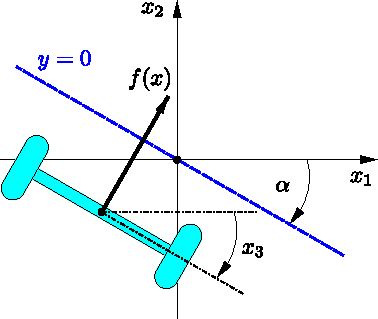
\includegraphics[width=0.5\textwidth]{Roboter_rel_Grad_mod}
\par\end{centering}
\caption{Roboter mit einem nicht überall wohldefinierten relativen Grad\label{fig:Roboter-rel-grad-gerade}}
\end{figure}

Ist die Bedingung~\ref{enu:rel-deg1} aus Definition~\ref{def:relativer-Grad-SISO}
für alle $k\in\NN$ erfüllt, dann definieren etliche Autoren einen
relativen Grad $r=\infty$, z.\,B.~\cite[Def.~{6.177}]{kwatny2000}.
Dieser Fall ist so zu verstehen, dass sich der Ausgang~$y$ in keiner
Weise durch den Eingang~$u$ beeinflussen lässt, also im System keine
,,interne`` Verbindung zwischen Eingang und Ausgang besteht. Das
trifft beispielsweise auf ein autonomes System $\dot{x}=f(x)$ zu.
Zusätzlich wird im nächsten Beispiel (wieder) der Spezialfall eines
linearen Systems behandelt. 
\begin{example}
\label{exa:Lineares-System-r-infty}Das lineare System~(\ref{eq:rel-grad-lineares-system})
aus Anmerkung~\ref{rem:rel-grad-Markovparameter} liege in einer
\emph{Kalman-Zerlegung}\index{Kalman-Zerlegung} 
\begin{eqnarray*}
\left(\begin{array}{c}
\dot{x}_{1}\\
\dot{x}_{2}\\
\dot{x}_{3}\\
\dot{x}_{4}
\end{array}\right) & = & \left(\begin{array}{cccc}
A_{11} & A_{12} & A_{13} & A_{14}\\
0 & A_{22} & 0 & A_{24}\\
0 & 0 & A_{33} & A_{34}\\
0 & 0 & 0 & A_{44}
\end{array}\right)\left(\begin{array}{c}
x_{1}\\
x_{2}\\
x_{3}\\
x_{3}
\end{array}\right)+\left(\begin{array}{c}
b_{1}\\
b_{2}\\
0\\
0
\end{array}\right)u\\
y & = & \left(\begin{array}{cccc}
0 & c_{2}^{T} & 0 & c_{4}^{T}\end{array}\right)x
\end{eqnarray*}
mit geeigneten Matrizen~$A_{11},A_{12},\ldots,A_{44}$ und passenden
Vektoren $b_{1},b_{2,}c_{2},c_{4}$ vor~\cite{lunze-rt2}. Dabei
sind das erste und zweite Teilsystem steuerbar sowie das zweite und
vierte Teilsystem beobachtbar. Das Eingangs-Ausgangs-Verhalten, welches
sich beispielsweise durch die Übertragungsfunktion beschreiben lässt,
hängt nur vom zweiten Teilsystem, das sowohl steuer- als auch beobachtbar
ist, ab~\cite{kalman1962canonical,lunze-rt2}. Das ist auch anhand
der gemischten Lie-Ableitungen bzw. der Markovparameter\index{Markovparameter}
zu erkennen: 
\[
L_{g}L_{f}^{k}h(x)=c^{T}A^{k}b=c_{2}^{T}A_{22}^{k}b_{2}.
\]
Die gemischte Lie-Ableitung des linearen Systems nimmt nur dann einen
von Null verschiedenen Wert an, wenn es ein gleichzeitig steuer- als
auch beobachtbares Teilsystem gibt. Andernfalls würde man im o.\,g.
Sinne $r=\infty$ erhalten.

\end{example}
\medskip{}

Das allgemeine Vorgehen beim Reglerentwurf für ein System~(\ref{eq:Ausgangssystem-fuer-BINF})
mit relativem Grad~$r$ lässt sich auf Basis von Gl.~(\ref{eq:rg-yrdot})
beschreiben. Der Reglerentwurf erfolgt in zwei Schritten:
\begin{enumerate}
\item Linearisierung durch Rückführung,
\item Stabilisierung des linearisierten Systems.
\end{enumerate}
Im ersten Schritt setzt man die rechte Seite von Gl.~(\ref{eq:rg-yrdot})
einer neuen Systemgröße~$v$ gleich, d.\,h. 
\begin{equation}
L_{f}^{r}h(x)+L_{g}L_{f}^{r-1}h(x)u\stackrel{!}{=}v,\label{eq:regler1-linearisierung-forderung}
\end{equation}
so kann man die Gleichung wegen $L_{g}L_{f}^{r-1}h(p)\neq0$ in einer
Umgebung von~$p$ nach~$u$ umstellen: 
\begin{equation}
u=\frac{1}{L_{g}L_{f}^{r-1}h(x)}\left(v-L_{f}^{r}h(x)\right).\label{eq:regler1-linearisierung}
\end{equation}
Die Systemgröße~$v$ lässt sich als neuer (virtueller) Eingang interpretieren.
Gl.~(\ref{eq:regler1-linearisierung}) beschreibt dann eine Zustandsrückführung
(siehe Abb.~\ref{fig:linearisierende-Zustandsrueckfuehrung}), mit
der Gleichung~(\ref{eq:rg-yrdot}) die Form einer Integratorkette
annimmt: 
\begin{equation}
y^{(r)}=v.\label{eq:regler-integratorkette}
\end{equation}
Durch die Rückführung~(\ref{eq:regler1-linearisierung}) werden die
in Gl.~(\ref{eq:rg-yrdot}) auftretenden Nichtlinearitäten kompensiert,
so dass man das lineare System~(\ref{eq:regler-integratorkette})
und damit ein lineares Eingangs-Ausgangs-Verhalten erhält. Man spricht
daher von einer \emph{Eingangs-Ausgangs-Linearisierung}. Die Rückführung~(\ref{eq:regler1-linearisierung})
nennt man auch \emph{linearisierende Rückführung}.

\begin{figure}
\begin{centering}
\resizebox{0.99\textwidth}{!}{\input{linearisierende-rueckfuehrung.pdftex_t}}
\par\end{centering}
\caption{Linearisierende Zustandsrückführung~(\ref{eq:regler1-linearisierung})\label{fig:linearisierende-Zustandsrueckfuehrung}}
\end{figure}

\begin{remark}
\label{rem:Hirschorn-Inverse}Das System~(\ref{eq:Ausgangssystem-fuer-BINF})
liefert das Ausgangssignal~$y$ als Antwort auf die Erregung durch
das Eingangssignal~$u$. Gibt man umgekehrt einen gewünschten Verlauf
des Ausgangssignals in Form einer $r$-mal stetig differenzierbaren
Funktion~$y$ vor, so kann man bei einem bekannten Verlauf des Zustands~$x$
durch Einsetzen von~(\ref{eq:regler-integratorkette}) in~(\ref{eq:regler1-linearisierung})
den zugehörigen Verlauf des Eingangssignals~$u$ ermitteln: 
\begin{equation}
u=\frac{1}{L_{g}L_{f}^{r-1}h(x)}\left(y^{(r)}-L_{f}^{r}h(x)\right).\label{eq:hirschorn-inverse-SISO}
\end{equation}
Mit Gl.~(\ref{eq:hirschorn-inverse-SISO}) wird (bei konsistenten
Anfangswerten) die Systemdynamik von~(\ref{eq:Ausgangssystem-fuer-BINF})
invertiert. Bei genauerer Betrachtung handelt es sich bei~(\ref{eq:hirschorn-inverse-SISO})
um eine \emph{Rechtsinverse}\index{Rechtsinverse} des Systems~(\ref{eq:Ausgangssystem-fuer-BINF}),
vgl. Abb.~\ref{fig:rechtsinverse-hirschon}. Die Inverse~(\ref{eq:hirschorn-inverse-SISO})
bzw. Gl.~(\ref{eq:regler1-linearisierung}) nennt man auch \emph{Hirschorn-Inverse}\index{Hirschorn-Inverse}~\cite{hirschorn1979,daoutidis1991,henson1997chap3}.
\end{remark}
\begin{figure}
\begin{centering}
\resizebox{0.99\textwidth}{!}{\input{hirschorn-inverse.pdftex_t}}
\par\end{centering}
\caption{Rechtsinverse~(\ref{eq:hirschorn-inverse-SISO}) des Systems~(\ref{eq:Ausgangssystem-fuer-BINF})\label{fig:rechtsinverse-hirschon}}
\end{figure}

Das durch Gl.~(\ref{eq:regler-integratorkette}) beschriebene Übertragungsglied
ist linear, aber instabil~\cite{reinschke2014buch}. Die zusätzliche
Rückführung 
\begin{equation}
v=-\sum_{k=0}^{r-1}a_{k}y^{(k)}\label{eq:regler2-stabilisierung}
\end{equation}
führt auf die lineare zeitinvariante Differentialgleichung 
\begin{equation}
y^{(r)}+a_{r-1}y^{(r-1)}+\cdots+a_{1}\dot{y}+a_{0}y=0.\label{eq:lineare-dgl-ordnung-r}
\end{equation}
Die Koeffizienten $a_{0},\ldots,a_{r-1}\in\R$ kann man so wählen,
dass alle Lösungen der zugehörigen charakteristischen Gleichung 
\begin{equation}
s^{r}+a_{r-1}s^{r-1}+\cdots+a_{1}s+a_{0}=0\label{eq:rg-gl-char-gleichung}
\end{equation}
negativen Realteil aufweisen. Ein solches charakteristisches Polynom
nennt man \emph{stabiles Polynom} oder \emph{Hurwitz-Polynom}\index{Hurwitz-Polynom}.
Dazu gibt man $r$ Nullstellen $s_{1},\ldots,s_{r}$ mit negativem
Realteil vor, wobei die Nullstellen reell sind oder in konjugiert
komplexen Paaren auftreten. Die Koeffizienten $a_{0},\ldots,a_{r-1}$
ergeben sich aus einem Koeffizientenvergleich: 
\[
(s-s_{1})\cdots(s-s_{r})\stackrel{!}{=}s^{r}+a_{r-1}s^{r-1}+\cdots+a_{1}s+a_{0}.
\]
Die Rückführung~(\ref{eq:regler2-stabilisierung}) stabilisiert in
diesem Fall das System und wird daher auch \emph{stabilisierende Rückführung}
genannt.

Die beiden Entwurfsschritte lassen sich einerseits zusammenfassen,
andererseits kann man Gl.~(\ref{eq:regler2-stabilisierung}) auch
über den Zustand~$x$ ausdrücken. Die Kombination von Gln.~(\ref{eq:regler1-linearisierung})
und~(\ref{eq:regler2-stabilisierung}) in Verbindung mit $y^{(k)}=L_{f}^{k}h(x)$
für $k=0,\ldots,r-1$ liefert die Zustandsrückführung 
\begin{equation}
u=-\frac{1}{L_{g}L_{f}^{r-1}h(x)}\sum_{k=0}^{r}a_{k}L_{f}^{k}h(x)\quad\text{mit}\quad a_{r}:=1.\label{eq:regler3-linearisierung-stabilisierung}
\end{equation}

Die Rückführung~(\ref{eq:regler3-linearisierung-stabilisierung})
stabilisiert die Ruhelage $y=0$ der Differentialgleichung~(\ref{eq:lineare-dgl-ordnung-r}).
Möchte man stattdessen für die Regelgröße~$y$ einen gewünschten
Sollwert vorgeben, so erweitert man die stabilisieriende Rückführung~(\ref{eq:regler2-stabilisierung})
um die Führungsgröße~$w$ zu 
\begin{equation}
v=a_{0}w-\sum_{k=0}^{r-1}a_{k}y^{(k)}.\label{eq:regler4-linearisierung-stabilisierung-sollwert-y}
\end{equation}
Ersetzt man die Zeitableitungen des Ausgangs durch die entsprechenden
Lie-Ableitungen, so lässt sich das Regelgesetz~(\ref{eq:regler4-linearisierung-stabilisierung-sollwert-y})
analog zu~(\ref{eq:regler3-linearisierung-stabilisierung}) als Zustandsrückführung
\begin{equation}
u=\frac{1}{L_{g}L_{f}^{r-1}h(x)}\left(a_{0}w-\sum_{k=0}^{r}a_{k}L_{f}^{k}h(x)\right)\label{eq:regler4-linearisierung-stabilisierung-sollwert-x}
\end{equation}
angeben. Mit der Rückführung~(\ref{eq:regler4-linearisierung-stabilisierung-sollwert-y})
bzw.~(\ref{eq:regler4-linearisierung-stabilisierung-sollwert-x})
erhält man die lineare Differentialgleichung 
\begin{equation}
y^{(r)}+a_{r-1}y^{(r-1)}+\cdots+a_{1}\dot{y}+a_{0}y=a_{0}w,\label{eq:lineare-dgl-ordnung-r-mit-w}
\end{equation}
siehe Abb.~\ref{fig:regelungsnormalform-lin-stab-w}. Der Faktor
vor der Führungsgröße~$w$ wurde so gewählt, dass bei konstantem~$w$
die Differentialgleichung~(\ref{eq:lineare-dgl-ordnung-r-mit-w})
die Ruhelage $y=w$ besitzt. Der gewünschte Sollwert~$w$ stellt
sich damit am Ausgang (asymptotisch) ein. Der Faktor $a_{0}$ agiert
in diesem Zusammenhang als (statisches) Vorfilter zur Sicherung des
jeweils gegebenen Sollwertes (siehe~\cite[Abschnitt~{4.4.2}]{lunze-rt2}).
Zwischen der Führungsgröße~$w$ und der Regel- bzw. Ausgangs\-größe~$y$
wirkt im Frequenzbereich (also zwischen den Laplace-Transformierten
$W$ und $Y$ der Signale~$w$ und~$y$) die Übertragungsfunktion
\begin{equation}
G_{W}^{Y}(s)=\frac{Y(s)}{W(s)}=\frac{a_{0}}{s^{r}+a_{r-1}s^{r-1}+\cdots+a_{1}s+a_{0}}.\label{eq:UF-WY}
\end{equation}
Die Stabilität dieses Übertragungsgliedes lässt sich durch die Wahl
der Koeffizienten $a_{0},\ldots,a_{n-1}$ sicherstellen. 

\begin{figure}
\begin{centering}
\resizebox{0.85\textwidth}{!}{\input{regelungsnormalform-lin-stab-w.pdftex_t}}
\par\end{centering}
\caption{Stabilisiertes Regelungssystem~(\ref{eq:lineare-dgl-ordnung-r-mit-w})\label{fig:regelungsnormalform-lin-stab-w}}
\end{figure}

\begin{example}
\label{exa:Roboter-geregelt1}Man betrachte den mobilen Roboter aus
Beispiel~\ref{exa:Roboter-rel-grad}. Für den Ausgang~(\ref{eq:roboter-rg-ausgang})
setzen wir $c_{1}=1$ und $c_{2}=0$. Der Ausgang $y=h(x)=x_{1}$
gibt in diesem Fall die $x_{1}$-Position des Roboters an. Die gemischte
Lie-Ableitung besitzt dann die Form $L_{g}L_{f}h(x)=\cos x_{3}$,
so dass der relative Grad $r=2$ für $x_{3}\notin\{\pi/2+k\pi,\,k\in\Z\}$
wohldefiniert ist. Zu entwerfen ist ein Regelgesetz, welches den Roboter
auf eine durch die Führungsgröße~$w$ vorgegebene $x_{1}$-Position
führt und diese Lage stabilisert. Aus Gl.~(\ref{eq:regler4-linearisierung-stabilisierung-sollwert-x})
ergibt sich die nichtlineare Zustandsrückführung 
\begin{eqnarray*}
u & = & \frac{1}{L_{g}L_{f}h(x)}\left(a_{0}\left(w-h(x)\right)-a_{1}L_{f}h(x)-L_{f}^{2}h(x)\right)\\
 & = & \frac{1}{\cos x_{3}}\left(a_{0}(w-x_{1})-a_{1}\sin x_{3}\right)
\end{eqnarray*}
mit den Koeffizienten $a_{0}$ und $a_{1}$. Für die Führungsübertragungsfunktion
geben wir eine doppelte Polstelle bei $s_{1,2}=-1$ vor, so dass man
aus $(s+1)^{2}=s^{2}+2s+1$ für die charakteristische Gleichung~(\ref{eq:rg-gl-char-gleichung})
die Koeffizienten $a_{0}=1$ und $a_{1}=2$ abliest. Abb.~\ref{fig:Roboter-geregelt1}
zeigt die Simulationsergebnisse des geregelten Robotermodells für
die Anfangswerte $x_{1}(0)=2$, $x_{2}(0)=1$, $x_{3}(0)=\pi/4$ ($\widehat{=}\,45\text{°}$)
und die Führungsgröße $w=1$. Die Konvergenz $y(t)=x_{1}(t)\to w=1$
für $t\to\infty$ ist visuell zu erkennen. Allerdings strebt der Roboter
nicht gegen eine Ruhelage, da er seine Fahrt (wegen der Annahme einer
konstanten Geschwindigkeit) parallel zur $x_{2}$-Achse fortsetzt.
\end{example}
\begin{figure}
\begin{centering}
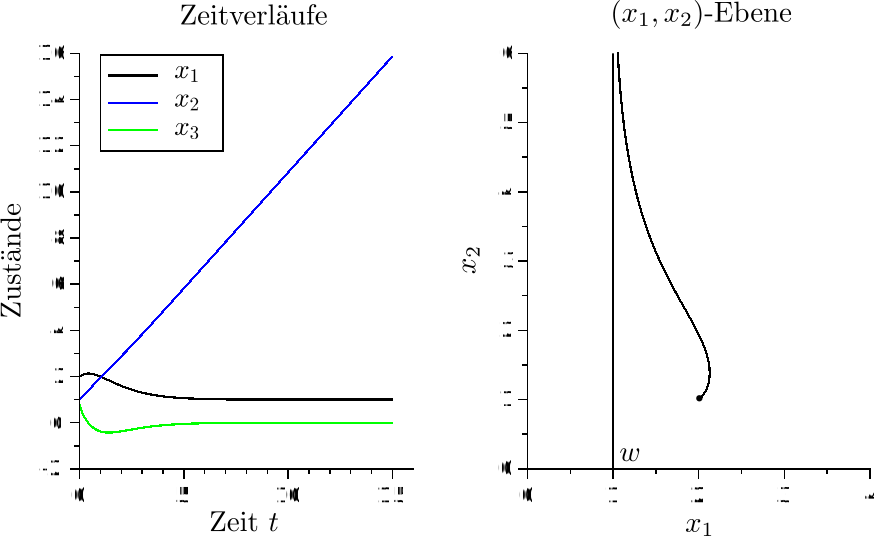
\includegraphics[width=0.85\textwidth]{robot_lin}
\par\end{centering}
\caption{Trajektorien des geregelten mobiler Robotermodells aus Beispiel~\ref{exa:Roboter-geregelt1}\label{fig:Roboter-geregelt1}}
\end{figure}

Den bisherigen Stabilitätsüberlegungen lagen die linearen Differentialgleichungen~(\ref{eq:lineare-dgl-ordnung-r})
bzw.~(\ref{eq:lineare-dgl-ordnung-r-mit-w}) zugrunde. Wenn der relative
Grad kleiner ist als die System\-ordnung, also für $r<n$, erfassen
diese Gleichungen nicht die komplette System\-dynamik. Daher spricht
man bei der Eingangs-Ausgangs-Linearisierung auch von einer \emph{partiellen
Linearisierung}.\index{partielle Linearisierung}\index{Linearisierung!partielle}
Die Betrachtung der gesamten System\-dynamik im Zustandsraum erfolgt
in Abschnitt~\ref{subsec:Byrnes-Isidori-Normalform}. Bei $r=n$
erzielt man eine vollständige Linearisierung, die sog. \emph{Eingangs-Zustands-Linearisierung},
die in Abschnitt~\ref{sec:Exakte-Eingangs-Zustands-Linearisierung}
behandelt wird.

Bei einer partiellen Linearisierung erhält man gerade bei mechanischen
Systemen oft deutlich einfache Differentialgleichungen, so dass dieser
Zugang auch für andere (z.\,B. energiebasierte) Regelungsansätze
hilfreich ist~\cite{spong1996}.

\begin{example}
\label{exa:Wagen-Pendel-partielle-Linearisierung}Das in Abschnitt~\ref{subsec:Wagen-mit-Pendel}
vorgestellte Wagen-Pendel-System wird durch die nicht ganz einfachen
Zustandsgleichungen
\begin{equation}
\begin{array}{lcl}
\dot{x}_{1} & = & x_{2}\\
\dot{x}_{2} & = & \frac{m_{2}\ell^{2}x_{4}^{2}\sin x_{3}-d_{1}\ell x_{2}+\cos x_{3}\left(m_{2}g\ell\sin x_{3}+d_{2}x_{4}\right)+\ell u}{\ell\left(m_{1}+m_{2}\sin^{2}x_{3}\right)}\\
\dot{x}_{3} & = & x_{4}\\
\dot{x}_{4} & = & \frac{-\left(m_{1}+m_{2}\right)\left(m_{2}g\ell\sin x_{3}+d_{2}x_{4}\right)-\cos x_{3}\left(\ell^{2}m_{2}^{2}x_{4}^{2}\sin x_{3}-d_{1}\ell m_{2}x_{2}\right)-\ell m_{2}u\cos x_{3}}{\ell^{2}m_{2}\left(m_{1}+m_{2}\sin^{2}x_{3}\right)}
\end{array}\label{eq:wagen-pendel-regler-grundlagen}
\end{equation}
beschrieben. Verwendet man als Ausgang die Position des Wagens, so
tritt der Eingang~$u$ erst in der zweiten Zeitableitung auf:
\begin{equation}
\begin{array}{lclclcl}
y & = & x_{1}\\
\dot{y} & = & \dot{x}_{1} & = & x_{2}\\
\ddot{y} & = & \dot{x}_{2} & = & \frac{m_{2}\ell^{2}x_{4}^{2}\sin x_{3}-d_{1}\ell x_{2}+\cos x_{3}\left(m_{2}g\ell\sin x_{3}+d_{2}x_{4}\right)+\ell u}{\ell\left(m_{1}+m_{2}\sin^{2}x_{3}\right)} & \stackrel{!}{=} & v.
\end{array}\label{eq:wagen-pendel-zeitableitungen}
\end{equation}
Eine partielle Linearisierung erzielt man, indem man die letzte Gleichung
nach dem Eingang~$u$ umstellt: 
\begin{equation}
u=v\left(m_{1}+m_{2}\sin^{2}x_{3}\right)-m_{2}\sin x_{3}\left(\ell x_{4}^{2}+g\cos x_{3}\right)+d_{1}x_{2}-\frac{d_{2}}{\ell}x_{4}\cos x_{3}.\label{eq:wagen-pendel-u-partiell-lin}
\end{equation}
Das entspricht formal dem Übergang von~(\ref{eq:regler1-linearisierung-forderung})
zu~(\ref{eq:regler1-linearisierung}). Setzt man~(\ref{eq:wagen-pendel-u-partiell-lin})
in Gl.~(\ref{eq:wagen-pendel-regler-grundlagen}) ein, so vereinfacht
sich nicht nur die zweite, sondern auch die vierte Gleichung von~(\ref{eq:wagen-pendel-regler-grundlagen}).
Insgesamt erhält man das folgende partiell linearisierte System\foreignlanguage{english}{:}
\begin{equation}
\begin{array}{lcl}
\dot{x}_{1} & = & x_{2}\\
\dot{x}_{2} & = & v\\
\dot{x}_{3} & = & x_{4}\\
\dot{x}_{4} & = & -\frac{d_{2}}{\ell^{2}m_{2}}x_{4}-\frac{g}{\ell}\sin x_{3}-\frac{1}{\ell}v\cos x_{3}\\
y & = & x_{1}.
\end{array}\label{eq:wagen-pendel-kollokiert-linearisiert}
\end{equation}
\end{example}

Wenn bei der Eingangs-Ausgangs-Linearisierung eines mechanischen Systems
Eingang und Ausgang die gleiche Konfigurationskoordinate (bzw. das
gleiche Gelenk) betreffen, dann spricht man von einer \emph{kollokierten}\index{Linearisierung!kollokierte},
andernfalls von einer \emph{nicht-kollokierten} partiellen Linearisierung~\cite{spong1994,spong1998}.
In Beispiel~\ref{exa:Wagen-Pendel-partielle-Linearisierung} wird
bezüglich der Koordinate~$q_{1}$ eine kollokierte Linearisierung
vorgenommen. Hätte man stattdessen $q_{2}=x_{3}$ als Ausgang verwendet,
so würde eine nicht-kollokierte Linearisierung vorliegen.

\subsection{Byrnes-Isidori-Normalform\label{subsec:Byrnes-Isidori-Normalform}}

Dieser Abschnitt befasst sich mit der Transformation eines gegebenen
Systems~(\ref{eq:Ausgangssystem-fuer-BINF}) in eine Form, die sowohl
zur Untersuchung des Eingangs-Ausgangs-Verhaltens als auch für die
Beschreibung des geregelten Systems sinnvoll ist. Bei der herzuleitenden
Transformation kommt dem relativen Grad eine besondere Bedeutung zu.
In diesem Abschnitt gehen wir davon aus, dass das System~(\ref{eq:Ausgangssystem-fuer-BINF})
im Punkt $p\in\mathcal{M}$ den wohldefinierten relativen Grad~$r$
besitzt. 

Bei den in der Definition des relativen Grades auftretenden gemischten
Lie-Ableitungen $L_{g}L_{f}^{i}h$ wird von dem Skalarfeld~$h$ eine
Lie-Ableitung der Ordnung $i+1$ gebildet, nämlich $i$ mal in Richtung
des Vektorfeldes~$f$ und einmal in Richtung des Vektorfeldes~$g$.
Das folgende Lemma besagt, dass man die Ableitungsordnung für das
Skalarfeldes~$h$ reduzieren kann, wenn man statt dessen entsprechende
Lie-Ableitungen des Vektorfeldes~$g$ (also Lie-Klammern) bildet.
Diese Hilfsaussage wird auch für die Eingangs-Zustands-Linearisierung
benötigt (siehe Abschnitt~\ref{sec:Exakte-Eingangs-Zustands-Linearisierung}).
\begin{lemma}
\label{lem:Skalarprod-dLf-ad}In einer Umgebung von~$p$ gilt 
\begin{equation}
\left\langle \d L_{f}^{j}h,\ad_{-f}^{i}g\right\rangle =\left\{ \begin{array}{ccccc}
0 & \mbox{für} & i+j & < & r-1,\\
L_{g}L_{f}^{r-1}h & \mbox{für} & i+j & = & r-1.
\end{array}\right.\label{eq:SP-dLfj,adi}
\end{equation}
\end{lemma}
\begin{svmultproof2}
Wir beweisen die Aussage mit Induktion über~$i$ bei festem~$j$.
Induktionsanfang ($i=0$): Es gilt 
\[
\left\langle \d L_{f}^{j}h,g\right\rangle =L_{g}L_{f}^{j}h=\left\{ \begin{array}{ccccc}
0 & \mbox{für} & j & < & r-1,\\
L_{g}L_{f}^{r-1}h & \mbox{für} & j & = & r-1,
\end{array}\right.
\]
da das System~(\ref{eq:Ausgangssystem-fuer-BINF}) den relativen
Grad~$r$ besitzt. 

Gl.~(\ref{eq:SP-dLfj,adi}) gelte für $i=0,\ldots,k-1$ (Induktionsannahme).
Der Induktionsschritt für $k+j\leq r-1$ liefert
\[
\begin{array}{ccl}
\left\langle \d L_{f}^{j}h,\ad_{-f}^{k}g\right\rangle  & = & \d L_{f}^{j}h\cdot\ad_{-f}^{k}g\\
 & = & L_{\ad_{-f}^{k}g}L_{f}^{j}h\\
 & = & L_{[-f,\ad_{-f}^{k-1}g]}L_{f}^{j}h\\
 & = & -\underbrace{L_{f}L_{\ad_{-f}^{k-1}g}L_{f}^{j}h}_{{\displaystyle =0}}+L_{\ad_{-f}^{k}g}L_{f}L_{f}^{j}h,
\end{array}
\]
wobei der erste Summand nach Induktionsannahme Null ist. Damit gilt
weiter 
\[
\begin{array}{lcl}
\left\langle \d L_{f}^{j}h,\ad_{-f}^{k}g\right\rangle  & = & L_{\ad_{-f}^{k}g}L_{f}L_{f}^{j}h\\
 & = & L_{\ad_{-f}^{k}g}L_{f}^{j+1}h\\
 & = & \left\langle \d L_{f}^{j+1}h,\ad_{-f}^{k-1}g\right\rangle .
\end{array}
\]
An dieser Stelle bietet sich eine Fallunterscheidung an:

\begin{enumerate}
\item $k+j<r-1$. Das impliziert $(k-1)+(j+1)<r$, d.\,h. nach Induktionsannahme
gilt 
\[
\left\langle \d L_{f}^{j}h,\ad_{-f}^{k}g\right\rangle =\left\langle \d L_{f}^{j+1}h,\ad_{-f}^{k-1}g\right\rangle =0.
\]
\item $k+j=r-1$. Die Induktionsannahme liefert 
\begin{eqnarray*}
\left\langle \d L_{f}^{j}h,\ad_{-f}^{k}g\right\rangle  & = & \left\langle \d L_{f}^{j+1}h,\ad_{-f}^{k-1}g\right\rangle \\
 & \vdots\\
 & = & \left\langle \d L_{f}^{r-1}h,\ad_{-f}^{0}g\right\rangle \\
 & = & \left\langle \d L_{f}^{r-1}h,g\right\rangle \\
 & = & L_{g}L_{f}^{r-1}h.
\end{eqnarray*}
\end{enumerate}
Damit ist Lemma~\ref{lem:Skalarprod-dLf-ad} bewiesen.
\end{svmultproof2}

Die nächste Hilfsaussage bildet die Grundlage für die Konstruktion
eines $r$-dimensionalen ersten Teilsystems.
\begin{lemma}
\label{lem:Lin-Unabh-Kovektoren}Die Kovektoren 
\[
\d h(p),\,\d L_{f}h(p),\,\ldots,\,\d L_{f}^{r-1}h(p)
\]
sind linear unabhängig.
\end{lemma}
\begin{svmultproof2}
Wegen Lemma~\ref{lem:Skalarprod-dLf-ad} gilt
\begin{equation}
\begin{array}{l}
\left(\begin{array}{c}
\d h(p)\\
\d L_{f}h(p)\\
\vdots\\
\d L_{f}^{r-1}h(p)
\end{array}\right)\left(g(p),\ad_{-f}g(p),\ldots,\ad_{-f}^{r-1}g(p)\right)=\\
=\left(\begin{array}{cccc}
0 & \cdots & 0 & \langle\d h,\ad_{f}^{r-1}g\rangle(p)\\
\vdots & \qdots &  & *\\
0 &  & \qdots & \vdots\\
\langle\d L_{f}^{r-1}h,g\rangle(p) & * & \cdots & *
\end{array}\right)\\
=\left(\begin{array}{cccc}
0 & \cdots & 0 & L_{g}L_{f}^{r-1}h(p)\\
\vdots & \qdots &  & *\\
0 &  & \qdots & \vdots\\
L_{g}L_{f}^{r-1}h(p) & * & \cdots & *
\end{array}\right).
\end{array}\label{eq:Lin-Unabh-Kov-Beweis1}
\end{equation}
Wegen $L_{g}L_{f}^{r-1}h(p)\neq0$ ist die rechte Seite regulär mit
Rang~$r$. Daher müssen die Zeilen der Matrix 
\begin{equation}
\left(\begin{array}{c}
\d h(p)\\
\vdots\\
\d L_{f}^{r-1}h(p)
\end{array}\right)\label{eq:Lin-Unabh-Kov-Beweis2}
\end{equation}
linear unabhängig sein. 
\end{svmultproof2}

\begin{remark}
\label{rem:relativer-Grad-Systemordnung}Aus Lemma~\ref{lem:Lin-Unabh-Kovektoren}
folgt zusätzlich, dass der relative Grad~$r$ nicht die Systemdimension~$n$
übersteigen kann, also mit einem wohldefinierten relativen Grad~$r$
auch $r\leq n$ gilt: Angenommen, die Bedingungen aus Def.~\ref{def:relativer-Grad-SISO}
seien für eine natürliche Zahl $r>n$ erfüllt. Die rechte Seite von
Gl.~(\ref{eq:Lin-Unabh-Kov-Beweis1}) müsste dann den Rang $r>n$
haben. Das steht im Widerspruch zu der Aussage, dass die auf der linken
Seite von Gl.~(\ref{eq:Lin-Unabh-Kov-Beweis1}) als Faktor auftretende
$r\times n$-Matrix~(\ref{eq:Lin-Unabh-Kov-Beweis2}) höchsten den
Rang~$n$ besitzen kann.
\end{remark}

Auf Basis von Lemma~\ref{lem:Lin-Unabh-Kovektoren} lassen sich die
ersten $r$ Koordinaten einer neuen Zustandsraumdarstellung des Systems~(\ref{eq:Ausgangssystem-fuer-BINF})
angeben. Durch eine standardmäßige Basisergänzung um $n-r$ weitere
Koordinaten wird man auf die nachfolgend angegebene Zwischenform geführt~\cite{chen1996,devasia1996}:
\begin{theorem}
\label{thm:EA-Form}Wir setzen 
\begin{equation}
\begin{array}{lcl}
\phi_{1}(x) & = & h(x)\\
\phi_{2}(x) & = & L_{f}h(x)\\
 & \vdots\\
\phi_{r}(x) & = & L_{f}^{r-1}h(x).
\end{array}\label{eq:Phi1}
\end{equation}
Für $r<n$ gibt es $n-r$ weitere glatte Funktionen $\phi_{r+1},\ldots,\phi_{n}$,
so dass 
\begin{equation}
z=\Phi(x)=\left(\begin{array}{c}
\phi_{1}(x)\\
\vdots\\
\phi_{n}(x)
\end{array}\right)\label{eq:Phi}
\end{equation}
in der Umgebung des Punktes~$p$ ein lokaler Diffeomorphismus ist,
der das System~(\ref{eq:Ausgangssystem-fuer-BINF}) in die \emph{Eingangs-Ausgangs-Normalform}\index{Eingangs-Ausgangs-Normalform}\index{Normalform!Eingangs-Ausgangs-}\footnote{Unter einer \emph{Normalform} wird in diesem Buch die Darstellung
eines mathematischen Objektes mit vorgegebenen Eigenschaften verstanden.
Im Unterschied zu anderen Autoren wird hier keine Eindeutigkeit dieser
Darstellung gefordert.}
\begin{equation}
\begin{array}{lcl}
\dot{z}_{1} & = & z_{2}\\
 & \vdots\\
\dot{z}_{r-1} & = & z_{r}\\
\dot{z}_{r} & = & \alpha(z)+\beta(z)u\\
\dot{z}_{r+1} & = & q_{1}(z)+d_{1}(z)u\\
 & \vdots\\
\dot{z}_{n} & = & q_{n-r}(z)+d_{n-r}(z)u\\
y & = & z_{1}
\end{array}\label{eq:EA-Form-komponentenweise}
\end{equation}
überführt.
\end{theorem}
\begin{svmultproof2}
Nach Lemma~\ref{lem:Lin-Unabh-Kovektoren} sind die Zeilenvektoren
$\d h(p),\ldots,\d L_{f}^{r-1}h(p)\in(\R^{n})^{*}$ linear unabhängig.
Diese Kovektoren spannen einen $r$-dimensionalen Unterraum~$\mathbb{U}$
im Dualraum~$(\R^{n})^{*}$ auf. Der zugehörige \index{Annihilatorraum}Annihilatorraum~$\mathbb{U}^{\perp}$
ist ein $(n-r)$-dimensionaler Unterraum des~$\R^{n}$ und habe die
Basis $b_{1},\ldots,b_{n-r}\in\R^{n}$, d.\,h. $\mathbb{U}^{\perp}=\spann\{b_{1},\ldots,b_{n-r}\}$.
Die Funktionen~(\ref{eq:Phi1}) ergänzen wir durch die linearen Funktionen
\begin{equation}
\begin{array}{rcl}
\phi_{r+1}(x) & = & b_{1}^{T}x,\\
 & \vdots\\
\phi_{n}(x) & = & b_{n-r}^{T}x.
\end{array}\label{eq:Phi2}
\end{equation}
 Die Jacobimatrix 
\[
\Phi^{\prime}(p)=\left(\begin{array}{c}
\D h(p)\\
\vdots\\
\D L_{f}^{r-1}h(p)\\
\hline b_{1}^{T}\\
\vdots\\
b_{n-r}^{T}
\end{array}\right)\in\R^{n\times n}
\]
der Abbildung~$\Phi$ ist im Punkt~$p$ aufgrund des Dimensionssatzes
regulär (vgl. Abschnitt~\ref{sec:Lineare-Algebra}). Nach dem Satz
über die Umkehrfunktion ist $z=\Phi(x)$ ein lokaler Diffeomorphismus.\footnote{Mit der linearen Unabhängigkeit der Gradienten $\d h(p),\ldots,\d L_{f}^{r-1}h(p)$
wäre die Existenz eines lokalen Diffeomorphismus bereits nach Korollar~\ref{cor:ergaenzung-einer-kodistribution-integrierbar}
gesichert. Das hier beschriebene Vorgehen ist jedoch in Hinblick auf
die Berechnung der Koordinatentransformation einfacher.} 

Nun ist zu zeigen, dass das transformierte System die Form~(\ref{eq:EA-Form-komponentenweise})
besitzt. Zunächst betrachten wir die Koordinaten $z_{i}=\phi_{i}(x)=L_{f}^{i-1}h(x)$
mit $i=1,\ldots,r$ des ersten Teilsystems von~(\ref{eq:EA-Form-komponentenweise}).
Für $i=1,\ldots,r-1$ gilt 
\begin{eqnarray*}
\dot{z}_{i} & = & \frac{\d}{\d t}\phi_{i}(x)\\
 & = & \d\phi_{i}(x)\cdot\dot{x}\\
 & = & \d L_{f}^{i-1}h(x)\cdot\left(f(x)+g(x)u\right)\\
 & = & L_{f}^{i}h(x)+\underbrace{L_{g}L_{f}^{i-1}h(x)}_{{\displaystyle \equiv0\mbox{ da }i<r}}u\\
 & = & \phi_{i+1}(x)\\
 & = & z_{i+1}.
\end{eqnarray*}
Bei $i=r$ gilt 
\begin{eqnarray*}
\dot{z}_{r} & = & \frac{\d}{\d t}\phi_{r}(x)\\
 & = & \d\phi_{r}(x)\cdot\dot{x}\\
 & = & \d L_{f}^{r-1}h(x)\cdot\left(f(x)+g(x)u\right)\\
 & = & L_{f}^{r}h(x)+\underbrace{L_{g}L_{f}^{r-1}h(x)}_{{\displaystyle \neq0}}u.
\end{eqnarray*}
Ein Vergleich mit Zeile~$r$ des Systems~(\ref{eq:EA-Form-komponentenweise})
liefert
\begin{equation}
\begin{array}{lcl}
\alpha(z) & = & \left.L_{f}^{r}h(x)\right|_{x=\Phi^{-1}(z)}\\
\beta(z) & = & \left.L_{g}L_{f}^{r-1}h(x)\right|_{x=\Phi^{-1}(z)}.
\end{array}\label{eq:alpha-beta-EA-NF}
\end{equation}

Anschließend betrachten wir die Koordinaten $z_{i}=\phi_{i}(x)$ mit
$i=r+1,\ldots,n$ des zweiten Teilsystems von~(\ref{eq:EA-Form-komponentenweise}).
Es gilt
\begin{eqnarray*}
\dot{z}_{i} & = & \frac{\d}{\d t}\phi_{i}(x)\\
 & = & \d\phi_{i}(x)\cdot\dot{x}\\
 & = & \d\phi_{i}(x)\cdot\left(f(x)+g(x)u\right)\\
 & = & L_{f}\phi_{i}(x)+L_{g}\phi_{i}(x)u.
\end{eqnarray*}
Die Funktionen $q_{1},\ldots,q_{n-r}$ und $d_{1},\ldots,d_{n-r}$
auf der rechten Seite der letzten $n-r$ Zeilen des Systems sind dementsprechend
durch
\[
\begin{array}{ccc}
q_{i}(z) & = & \left.L_{f}\phi_{r+i}(x)\right|_{x=\Phi^{-1}(z)}\\
d_{i}(z) & = & \left.L_{g}\phi_{r+i}(x)\right|_{x=\Phi^{-1}(z)}
\end{array}
\]
 für $i=1,\ldots,n-r$ definiert.
\end{svmultproof2}

\begin{remark}
Im Beweis wurde der von den Kovektoren $\d h(p),\ldots,\d L_{f}^{r-1}h(p)$
aufgespannte Unterraum $\mathbb{U}\subset(\R^{n})^{*}$ letztlich
durch sein orthogonales Komplement ergänzt. Alternativ ist auch die
Ergänzung durch eine geeignete Auswahl $\d x_{i_{1}},\ldots,\d x_{i_{n-r}}$
der kanonischen Basisvektoren möglich (Basis\-aus\-tausch\-satz
bzw. Aus\-tausch\-satz von Steinitz~\cite{kerner2007}), woraus
sich die zusätzlichen Funktionen $\phi_{r+1}(x)=x_{i_{1}},\ldots,\phi_{n}(x)=x_{i_{n-r}}$
ergeben. Bei diesem Zugang sind für das zweite Teilsystem keine neuen
Koordinaten festzulegen, sondern nur bestehende Koordinaten auszuwählen.
\end{remark}

Die im ersten Teilsystem der Eingangs-Ausgangs-Normalform~(\ref{eq:EA-Form-komponentenweise})
auftretenden Funktionen~$\alpha$ und~$\beta$ sind oft vergleichsweise
komplizierte Funktionen, die durch umfangreiche Ausdrücke beschrieben
werden. Da diese Nichtlinearitäten ohnehin kompensiert werden sollen
bietet es sich an, die Eingangs-Ausgangs-Linearisierung bereits \textit{vor}
der Berechnung der Normalform~(\ref{eq:EA-Form-komponentenweise})
durchzuführen. Nach einer solchen partiellen Linearisierung gilt $\alpha=0$
und $\beta=1$. 

\begin{example}
\label{exa:Wagen-Pendel-EA-NF}Man betrachte das Wagen-Pendel-System~(\ref{eq:wagen-pendel-regler-grundlagen})
aus Beispiel~\ref{exa:Wagen-Pendel-partielle-Linearisierung}. Die
partielle Linearisierung mit relativem Grad $r=2$ führt auf das deutlich
einfachere System~(\ref{eq:wagen-pendel-kollokiert-linearisiert}),
welches bereits in der Eingangs-Ausgangs-Normalform vorliegt. Dabei
wird das erste Teilsystem durch die Koordinaten $x_{1},x_{2}$ und
das zweite Teilsystem durch $x_{3},x_{4}$ beschrieben.
\end{example}

Mit der Eingangs-Ausgangs-Normalform zerfällt das System~(\ref{eq:Ausgangssystem-fuer-BINF})
in ein $r$-dimensionales erstes Teilsystem und ein $(n-r$)-dimensionales
zweites Teilsystem. Mit dem nächsten Lemma wird die Elimination des
Eingangs im zweiten Teilsystem ermöglicht~\cite[Prop.~{4.1.3}]{isidori3}.
\begin{lemma}
\label{lem:LgNull}Die ersten Koordinaten~(\ref{eq:Phi1}) können
durch zusätzliche Funktionen $\phi_{r+1},\ldots,\phi_{n}$ derart
ergänzt werden, dass die Abbildung~(\ref{eq:Phi}) im Punkt $p\in\mathcal{M}$
eine reguläre Jacobi\-matrix besitzt und außerdem 
\begin{equation}
L_{g}\phi_{i}(x)=0\quad\mbox{für}\quad i=r+1,\ldots,n\label{eq:Lg-phi}
\end{equation}
und alle~$x$ aus einer Umgebung von~$p$ gilt.
\end{lemma}

\begin{svmultproof2}
Aufgrund des wohldefinierten relativen Grades gilt $g(p)\neq0$. Dann
ist die Distribution $\Delta=\spann\{g\}$ regulär, und da sie eindimensional
ist auch involutiv: $[g,g]=0$. Der Satz von Frobenius (Satz~\ref{thm:Frobenius-lokal})
garantiert die Existenz von $n-1$ Skalarfeldern $\lambda_{1},\ldots,\lambda_{n-1}$
mit 
\begin{equation}
\Delta^{\perp}=\spann\{\d\lambda_{1},\ldots,\d\lambda_{n-1}\}\quad\text{und}\quad\dim(\Delta^{\perp})(p)=n-1.\label{eq:Annihil-n-1-fuer-BINF}
\end{equation}
Diese Skalarfelder erfüllen damit einerseits die Gleichung
\[
L_{g}\lambda_{i}(x)=0
\]
für $i=1,\ldots,n-1$ und alle~$x$ aus einer Umgebung von~$p$,
andererseits sind die Gradienten $\d\lambda_{i}$ im Punkt~$p$ linear
unabhängig (Dimensionsformel~(\ref{eq:dimensionssatz-distr-annihilator})
in Prop.~\ref{pro:Annihilator}). Wegen 
\[
\left\langle \d L_{f}^{k}h,g\right\rangle =L_{g}L_{f}^{k}h=0,\quad k=0,\ldots,r-2
\]
entsprechend Def.~\ref{def:relativer-Grad-SISO} sind bereits $r-1$
derartige Funktionen bekannt: $\lambda_{1}(x)=\phi_{1}(x)=h(x),\ldots,\lambda_{r-1}=\phi_{r-1}(x)=L_{f}^{r-2}h(x)$.
Die zugehörigen Gradienten sind zudem im Punkt~$p$ linear unabhängig
(Lemma~\ref{lem:Lin-Unabh-Kovektoren}). Damit existieren $(n-1)-(r-1)=n-r$
weitere (unabhängige) Funktionen $\phi_{r+1}(x)=\lambda_{r}(x),\ldots,\phi_{n}(x)=\lambda_{n-1}(x)$,
für welche Gl.~(\ref{eq:Annihil-n-1-fuer-BINF}) erfüllt ist. Außerdem
gilt aber auch 
\[
\left\langle \d L_{f}^{r-1}h,g\right\rangle =L_{g}L_{f}^{r-1}h(p)\neq0,
\]
so dass $\d L_{f}^{r-1}h$ nicht zum Annihiltor~$\Delta^{\perp}$
gehört. Damit gilt 
\[
\Delta^{\perp}(p)\oplus\spann\{\d L_{f}^{r-1}h(p)\}=(\R^{n})^{*},
\]
so dass mit $\phi_{r}(x)=L_{f}^{r-1}h(x)$ die Abbildung~$\Phi$
im Punkt~$p$ eine reguläre Jacobimatrix besitzt.
\end{svmultproof2}

Wählt man die Funktionen $\phi_{r+1},\ldots,\phi_{n}$ der Koordinatentransformation~(\ref{eq:Phi})
entsprechend Lemma~\ref{lem:LgNull}, dann geht die Eingangs-Ausgangs-Normalform
in die Byrnes-Isidori-Normalform über:
\begin{theorem}
\label{thm:Byrnes-Isidori-Normalform}Die in Lemma~\ref{lem:LgNull}
definierte Abbildung~$\Phi$ ist ein lokaler Diffeomorphismus, mit
dem System~(\ref{eq:Ausgangssystem-fuer-BINF}) in die \emph{Byrnes-Isidori-Normalform}\index{Normalform!Byrnes-Isidori-}\index{Byrnes-Isidori-Normalform}
\begin{equation}
\begin{array}{lcl}
\dot{z}_{1} & = & z_{2}\\
 & \vdots\\
\dot{z}_{r-1} & = & z_{r}\\
\dot{z}_{r} & = & \alpha(z)+\beta(z)u\\
\dot{z}_{r+1} & = & q_{1}(z)\\
 & \vdots\\
\dot{z}_{n} & = & q_{n-r}(z)\\
y & = & z_{1}
\end{array}\label{eq:BINF-Komponentenweise}
\end{equation}
überführt wird.
\end{theorem}
\begin{svmultproof2}
Bei wohldefiniertem relativen Grad~$r$ existiert nach Satz~\ref{thm:EA-Form}
die Eingangs-Ausgangs-Normalform~(\ref{eq:EA-Form-komponentenweise}).
Die ersten $r$ Koordinaten sind durch Gl.~(\ref{eq:Phi1}) gegeben.
Die zusätzlichen Koordinaten können entsprechend Gl.~(\ref{eq:Lg-phi})
gewählt werden (Lemma~\ref{lem:LgNull}). Für die Koordinaten $z_{i}=\phi_{i}(x)$
mit $i=r+1,\ldots,n$ des zweiten Teilsystems von~(\ref{eq:BINF-Komponentenweise})
gilt folglich
\begin{eqnarray*}
\dot{z}_{i} & = & \frac{\d}{\d t}\phi_{i}(x)\\
 & = & \d\phi_{i}(x)\cdot\dot{x}\\
 & = & \d\phi_{i}(x)\cdot\left(f(x)+g(x)u\right)\\
 & = & L_{f}\phi_{i}(x)+\underbrace{L_{g}\phi_{i}(x)}_{{\displaystyle \equiv\mbox{0}}}u\\
 & = & L_{f}\phi_{i}(x).
\end{eqnarray*}
Damit geht~(\ref{eq:EA-Form-komponentenweise}) in Gl.~(\ref{eq:BINF-Komponentenweise})
über, wobei das zweite Teilsystem nicht mehr direkt vom Eingang abhängt.
Die Funktionen $q_{1},\ldots,q_{n-r}$ auf der rechten Seite des zweiten
Teilsystems sind durch 
\[
q_{i}(z)=\left.L_{f}\phi_{r+i}(x)\right|_{x=\Phi^{-1}(z)}
\]
definiert.
\end{svmultproof2}

\begin{remark}
\label{rem:Berechnung-Byrnes-Isidori-NF}Für die Bestimmung der zusätzlichen
Funktionen $\phi_{r+1},\ldots,\phi_{n}$ kann man ausnutzen, dass
Lemma~\ref{lem:LgNull} mit dem Satz von Frobenius (Satz~\ref{thm:Frobenius-lokal})
bewiesen wurde, dessen Beweis konstruktiv mit Hilfe des Begradigungssatzes
(Satz~\ref{thm:simultane-begradigung-von-VF}) geführt wurde. Zur
Berechnung der gesuchten Funktionen ergänzt man das Eingangsvektorfeld
$g_{1}:=g$ um $n-1$ weitere (möglichst einfache) Vektorfelder $g_{2},\ldots,g_{n}$,
so dass alle Vektorfelder im Punkt~$p$ linear unabhängig sind. Dazu
kann man konstante Vektorfelder, insbesondere auch Einheitsvektorfelder
$\tfrac{\partial}{\partial x_{i}}$ verwenden. Die von diesen $n$
Vektorfeldern aufgespannte Distribution ist regulär und (da sie den
gesamten Raum aufspannt) involutiv. Wie in Gl.~(\ref{eq:S-flussverknuepfung})
des Beweises von Satz~\ref{thm:simultane-begradigung-von-VF} definiert
man über die Verkettung der Flüsse dieser Vektorfelder eine Abbildung\index{Fluss!Verkettung}
\begin{equation}
x=S(\tilde{z})=\varphi_{\tilde{z}_{1}}^{g_{1}}\circ\cdots\circ\varphi_{\tilde{z}_{n}}^{g_{n}}(p).\label{eq:flussverkettung-berechnung-BINF}
\end{equation}
Zu der Umkehrfunktion $\tilde{z}=T(x)$ betrachte man die Komponenten
$t_{2},\ldots,t_{n}$. Die zugehörigen Gradienten $\d t_{2},\ldots,\d t_{n}$
spannen in einer Umgebung des Punktes~$p$ den Annihilator von $\spann\{g\}$
auf (vgl. Beweis von Satz~\ref{thm:Frobenius-lokal}). Da die Gradienten
$\d h,\ldots,\d L_{f}^{r-2}h$ eine $r$-dimensionale Kodistribution
aufspannen, die im Annihilator enthalten ist, kann man von den Gradienten
$\d t_{2},\ldots,\d t_{n}$ genau $n-r$ Elemente zur Ergänzung der
Basis auswählen (Basis\-aus\-tausch\-satz bzw. Aus\-tausch\-satz
von Steinitz~\cite{kerner2007}).
\end{remark}

\begin{remark}
\label{rem:Berechnung-Byrnes-Isidori-NF-PDE}Formal stellt Gl.~(\ref{eq:Lg-phi})
eine \textit{partielle} Differentialgleichung dar, für die in Ergänzung
zu den bekannten Lösungen $h,L_{f}h,\ldots,L_{f}^{r-1}h$ (vgl. Punkt~\ref{enu:rel-deg1}
aus Def.~\ref{def:relativer-Grad-SISO}) noch $n-r$ weitere (unabhängige)
Lösungen $\phi_{r+1},\ldots,\phi_{n}$ gesucht sind. Grundsätzlich
bietet sich zur Lösung der partiellen Differentialgleichung~(\ref{eq:Lg-phi})
die Methode der Charakteristiken an~\cite{john1971}. Die symbolische
Lösung ist mit Computer-Algebra-Systemen nicht immer möglich~\cite{jager1991,jager95}. 
\end{remark}

Allerdings lassen sich in vielen Fällen die zusätzlichen Koordinaten
der Byrnes-Isidori-Normalform direkt angeben:

\begin{example}
\label{exa:Roboter-BI-NF}Man betrachte den mobilen Roboter aus Beispiel~\ref{exa:Roboter-rel-grad}
mit dem in Beispiel~\ref{exa:Roboter-geregelt1} verwendeten Ausgang
$y=x_{1}$. Der relative Grad $r=2$ ist für $x_{3}\notin\{\pi/2+k\pi,\,k\in\Z\}$
wohldefiniert. Die ersten $r$ Koordinaten der Byrnes-Isidori-Normalform
ergeben sich aus den Lie-Ableitungen
\begin{equation}
\begin{array}{lclcccl}
z_{1} & = & \phi_{1}(x) & = & h(x) & = & x_{1}\\
z_{2} & = & \phi_{2}(x) & = & L_{f}h(x) & = & \sin x_{3}.
\end{array}\label{eq:Roboter-BI-NF-hin1}
\end{equation}
Die dritte Koordinate muss von $x_{2}$ abhängen, andernfalls kann
die zur Koordinatentransformation gehörende Jacobimatrix nicht regulär
sein. Die lineare Funktion 
\begin{equation}
z_{3}=\phi_{3}(x)=x_{2}\label{eq:Roboter-BI-NF-hin2}
\end{equation}
erfüllt zudem noch die partielle Differentialgleichung~(\ref{eq:Lg-phi}).
Für $x_{3}\in(-\pi/2,+\pi/2)$ beschreiben die Gleichungen~(\ref{eq:Roboter-BI-NF-hin1})
und~(\ref{eq:Roboter-BI-NF-hin2}) einen Diffeomorphismus, dessen
Umkehrabbildung $z=\Phi^{-1}(x)$ durch 
\[
\begin{array}{lcl}
x_{1} & = & z_{1}\\
x_{2} & = & z_{3}\\
x_{3} & = & \arcsin z_{2}
\end{array}
\]
gegeben ist. Die Nichtlinearitäten~$\alpha$ und~$\beta$ des ersten
Teilsystems haben dann die Form 
\[
\alpha(z)=\left.L_{f}^{2}h(x)\right|_{x=\Phi^{-1}(z)}\equiv0
\]
und
\[
\beta(z)=\left.L_{g}L_{f}h(x)\right|_{x=\Phi^{-1}(z)}=\left.\cos x_{3}\right|_{x_{3}=\arcsin z_{2}}=\sqrt{1-z_{2}^{2}}\enspace.
\]
Für die Nichtlinearität des zweiten Teilsystems errechnet man 
\[
q_{1}(z)=\left.L_{f}\phi_{3}(x)\right|_{x=\Phi^{-1}(z)}=\left.\cos x_{3}\right|_{x_{3}=\arcsin z_{2}}=\sqrt{1-z_{2}^{2}}\enspace,
\]
so dass man insgesamt die Byrnes-Isidori-Normalform
\begin{equation}
\begin{array}{lcl}
\dot{z}_{1} & = & z_{2}\\
\dot{z}_{2} & = & \sqrt{1-z_{2}^{2}}\,u\\
\dot{z}_{3} & = & \sqrt{1-z_{2}^{2}}\\
y & = & z_{1}
\end{array}\label{eq:Roboter-BI-NF}
\end{equation}
mit einem zweidimensionalen ersten und einem eindimensionalen zweiten
Teilsystem erhält.
\end{example}

\begin{example}
\label{exa:Wagen-Pendel-System-BINF}Wir betrachten das partiell linearisierte
Wagen-Pendel-System~(\ref{eq:wagen-pendel-kollokiert-linearisiert})
aus Beispiel~\ref{exa:Wagen-Pendel-partielle-Linearisierung}. Das
System soll in die Byrnes-Isidori-Normalform transformiert werden.
Die ersten $r=2$ Koordinaten sind durch $z_{1}=h(x)=x_{1}$ und $z_{2}=L_{f}h(x)=x_{2}$
gegeben. Die zusätzlichen Koordinaten $z_{3}=\phi_{3}(x)$ und $z_{4}=\phi_{4}(x)$,
die die Bedingung~(\ref{eq:Lg-phi}) aus Lemma~\ref{lem:LgNull}
für das Eingangsvektorfeld
\begin{equation}
g(x)=\frac{\partial}{\partial x_{2}}-\frac{1}{\ell}\cos x_{3}\frac{\partial}{\partial x_{4}}\label{eq:wagen-pendel-vektorfeld-g-part-lin}
\end{equation}
des Systems~~(\ref{eq:wagen-pendel-kollokiert-linearisiert}) erfüllen,
werden systematisch entsprechend Anmerkung~\ref{rem:Berechnung-Byrnes-Isidori-NF}
bestimmt. Dazu ergänzen wir~(\ref{eq:wagen-pendel-vektorfeld-g-part-lin})
um die linear unabhängigen Basisvektorfelder $g_{2}=\tfrac{\partial}{\partial x_{1}}$,
$g_{3}=\tfrac{\partial}{\partial x_{3}}$ und $g_{4}=\tfrac{\partial}{\partial x_{4}}$,
deren Flüsse entsprechend Beispiel~\ref{exa:konstantes-Vektorfeld-Gruppeneig}
angegeben werden können. Die Verknüpfung der Flüsse nach Gl.~(\ref{eq:flussverkettung-berechnung-BINF})
mit $p=0$ liefert 
\[
\left.\begin{array}{lcl}
x_{1} & = & \tilde{z}_{2}\\
x_{2} & = & \tilde{z}_{1}\\
x_{3} & = & \tilde{z}_{3}\\
x_{4} & = & \tilde{z}_{4}-\frac{\tilde{z}_{1}}{\ell}\cos\tilde{z}_{3}
\end{array}\quad\right\} \quad x=S(\tilde{z})
\]
mit der Umkehrabbildung 
\[
\left.\begin{array}{lcl}
\tilde{z}_{1} & = & x_{2}\\
\tilde{z}_{2} & = & x_{1}\\
\tilde{z}_{3} & = & x_{3}\\
\tilde{z}_{4} & = & x_{4}+\frac{x_{2}}{\ell}\cos x_{3}
\end{array}\quad\right\} \quad\tilde{z}=T(x).
\]
Die erste Komponente liefert nach Konstruktion kein Element für den
Annihilator. Die zweite Komponente wird bereits im ersten Teilsystem
genutzt. Die zusätzlichen Koordinaten~$\phi_{3}$ und~$\phi_{4}$
ergeben sich daher aus den letzten zwei Komponenten~$t_{3}$ und~$t_{4}$.
Mit $z_{3}=\phi_{3}(x)=x_{3}$ und $z_{4}=\phi_{4}(x)=x_{4}+\tfrac{1}{\ell}x_{2}\cos x_{3}$
erhält man insgesamt die folgende Hin- bzw. Rücktransformation: 
\[
z=\Phi(x)=\left(\begin{array}{c}
x_{1}\\
x_{2}\\
x_{3}\\
x_{4}+\tfrac{1}{\ell}x_{2}\cos x_{3}
\end{array}\right),\quad x=\Phi^{-1}(z)=\left(\begin{array}{c}
z_{1}\\
z_{2}\\
z_{3}\\
z_{4}-\tfrac{1}{\ell}z_{2}\cos z_{3}
\end{array}\right).
\]
Durch Anwendung dieser Transformation wird das System~(\ref{eq:wagen-pendel-kollokiert-linearisiert})
in die Byrnes-Isidori-Normalform 
\begin{equation}
\begin{array}{lcl}
\dot{z}_{1} & = & z_{2}\\
\dot{z}_{2} & = & v\\
\dot{z}_{3} & = & \frac{z_{4}-z_{2}\cos z_{3}}{\ell}\\
\dot{z}_{4} & = & \frac{\left(d_{2}+\ell m_{2}z_{2}\sin z_{3}\right)\ell z_{4}+\left(g\ell-z_{2}^{2}\cos z_{3}\right)\ell m_{2}\sin z_{3}-d_{2}z_{2}\cos z_{3}}{\ell^{3}m_{2}}
\end{array}\label{eq:wagen-pendel-system-BINF}
\end{equation}
überführt. Im Unterschied zu der Eingangs-Ausgangs-Form~(\ref{eq:wagen-pendel-kollokiert-linearisiert})
tritt in dem durch die Koordinaten~$z_{3}$ und~$z_{4}$ beschriebenen
zweiten Teilsystem der Eingang~$v$ nicht mehr in Erscheinung.
\end{example}

\begin{remark}
Bei mechanischen Systemen führt eine kollokierte partielle Linearisierung
auf die Eingangs-Ausgangs-Normal\-form~(\ref{eq:EA-Form-komponentenweise}).
Auf Basis der Bewegungsgleichungen lässt sich dann ein globaler Diffeomorphismus
angeben, der~(\ref{eq:EA-Form-komponentenweise}) in die Byrnes-Isidori-Normalform~(\ref{eq:BINF-Komponentenweise})
überführt~\cite{knoll2015ssce,knoll2016diss}.
\end{remark}

\subsection{Reglerentwurf zur Stabilisierung einer Ruhelage\label{subsec:Reglerentwurf-zur-Stabilisierung-Ruhelage}}

Ein Punkt $(x^{0},u^{0})$ mit $x^{0}\in\mathcal{M}$ und $u^{0}\in\R$,
der die Gleichung 
\[
0=f(x^{0})+g(x^{0})u^{0}
\]
erfüllt, ist eine Ruhelage\index{Ruhelage} bzw. ein \index{Arbeitspunkt}Arbeitspunkt
des Systems~(\ref{eq:Ausgangssystem-fuer-BINF}). Zur Vereinfachung
gehen wir im Folgenden davon aus, dass die Ruhelage bei $x^{0}=p$
und $u^{0}=0$ liegt. In diesem Fall würden wir einfach von der Ruhelage
$p\in\mathcal{M}$ (ohne Erwähnung von~$u^{0}$) sprechen. Im Punkt
$p\in\mathcal{M}$ gelte somit 
\begin{eqnarray}
f(p) & = & 0,\label{eq:Ruhelage-x}\\
h(p) & = & 0.\label{eq:Ruhelage-y}
\end{eqnarray}
Der Ausgang sei dabei so gewählt, dass er in der Ruhelage auch den
Wert Null annimmt. Hat System~(\ref{eq:Ausgangssystem-fuer-BINF})
im Punkt~$p$ den relativen Grad~$r$, dann kann die Transformation~$\Phi$
in die Eingangs-Ausgangs- sowie Byrnes-Isidori-Normalform so gewählt
werden, dass zusätzlich $\Phi(p)=0$ gilt. Für $u=0$ ist dann $z=0$
die Ruhelage des transformierten Systems.

Die Eingangs-Ausgangs-Normalform~(\ref{eq:EA-Form-komponentenweise})
besteht aus zwei Teilsystemen. Dazu führen wir die Koordinaten 
\[
\begin{array}{lclcl}
\xi & = & (\xi_{1},\ldots,\xi_{r})^{T} & = & (z_{1},\ldots,z_{r})^{T}\\
\eta & = & (\eta_{1},\ldots,\eta_{n-r})^{T} & = & (z_{r+1},\ldots,z_{n})^{T}
\end{array}
\]
ein. Formal würde der Vektor~$z$ aus den übereinander anzuordnenden
Spaltenvektoren~$\xi$ und~$\eta$ bestehen. Im Sinne einer gut
lesbaren Notation werden wir aber den Zustandsvektor des Gesamtsystems
als geordnetes Paar $z=(\xi,\eta)$ angeben, was durch den Isomorphismus
$\R^{r}\times\R^{n-r}\cong\R^{n}$ gerechtfertigt ist. Diese Notation
ist sinngemäß auf die beteiligten Abbildungen zu übertragen. Die Eingangs-Ausgangs-Normalform~(\ref{eq:BINF-Komponentenweise})
lässt sich dann in der kompakten Form 
\begin{equation}
\begin{array}{rcl}
\dot{\xi} & = & A\xi+b(\alpha(\xi,\eta)+\beta(\xi,\eta)u)\\
\dot{\eta} & = & q(\xi,\eta)+d(\xi,\eta)u\\
y & = & c^{T}\xi
\end{array}\label{eq:EANF-Matrixform}
\end{equation}
mit 
\begin{equation}
A=\left(\begin{array}{cccc}
0 & 1 & \cdots & 0\\
0 & 0 & \ddots & \vdots\\
\vdots & \ddots & \ddots & 1\\
0 & \cdots & 0 & 0
\end{array}\right),\;b=\left(\begin{array}{c}
0\\
\vdots\\
0\\
1
\end{array}\right),\;c^{T}=\left(\begin{array}{cccc}
1 & 0 & \cdots & 0\end{array}\right)\label{eq:Abc-Brunovsky}
\end{equation}
angeben. Das Triple $(A,b,c^{T})$ mit $A=\R^{r\times r}$ und $b,c\in\R^{r}$
liegt in \emph{Brunovský-Normalform}\index{Brunovský-Normalform}\index{Normalform!Brunovský-}
vor~\cite{brunovsky70}. Für $d\equiv0$ geht die Eingangs-Ausgangs-Normalform~(\ref{eq:EANF-Matrixform})
in die Byrnes-Isidori-Normalform
\begin{equation}
\begin{array}{rcl}
\dot{\xi} & = & A\xi+b(\alpha(\xi,\eta)+\beta(\xi,\eta)u)\\
\dot{\eta} & = & q(\xi,\eta)\\
y & = & c^{T}\xi
\end{array}\label{eq:BINF-Matrixform}
\end{equation}
über, welche nachfolgend genutzt wird.

Das Vorgehen aus Abschnitt~\ref{subsec:Relativer-Grad-grundlegendes-Vorgehen}
kann jetzt im Zustandsraum des transformierten Systems~(\ref{eq:EANF-Matrixform})
erläutert werden. Die linearisierende Rückführung 
\begin{equation}
u=\frac{1}{\beta(\xi,\eta)}\left(v-\alpha(\xi,\eta)\right)=\frac{1}{L_{g}L_{f}^{r-1}h(x)}\left(v-L_{f}^{r}h(x)\right)\label{eq:rueckfuehrung-linearisierend}
\end{equation}
für das erste Teilsystem überführt die zugehörige Byrnes-Isidori-Normalform~(\ref{eq:BINF-Matrixform})
in das \emph{eingangs-ausgangs-linearisierte} oder \emph{partiell
linearisierte} System 
\begin{equation}
\begin{array}{rcll}
\dot{\xi} & = & A\xi+bv\qquad & \text{(lineares Teilsystem)}\\
\dot{\eta} & = & q(\xi,\eta) & \text{(interne Dynamik)}\\
y & = & c^{T}\xi.
\end{array}\label{eq:BINF-Linearisiert}
\end{equation}
mit einem linearen ersten Teilsystem und einem in der Regel nichtlinearen
zweiten Teilsystem, der sogenannten \emph{internen Dynamik}\index{interne Dynamik}.
Die interne Dynamik beeinflusst dann weder das erste Teilsystem noch
den Ausgang (Abb.~\ref{fig:eingangs-ausgangs-linearisiertes-system}).

\begin{figure}
\begin{centering}
\resizebox{0.9\textwidth}{!}{\input{integratorkette-exakte-linearisierung2.pdftex_t}}
\par\end{centering}
\caption{Eingangs-ausgangs-linearisiertes System~(\ref{eq:BINF-Linearisiert})
\label{fig:eingangs-ausgangs-linearisiertes-system}}
\end{figure}

Das Eingangs-Ausgangs-Verhalten von System~(\ref{eq:BINF-Linearisiert})
wird ausschließlich vom ersten Teilsystem bestimmt und lässt sich
durch die Übertragungsfunktion
\[
G_{V}^{Y}(s)=\frac{Y(s)}{V(s)}=c^{T}(sI-A)^{-1}b=\frac{1}{s^{r}}
\]
in Form eines $r$-fachen Integrators angeben. Im nächsten Schritt
soll das erste Teilsystem stabilisiert werden. Dazu setzt man die
Zustandsrückführung 
\begin{equation}
v=-k^{T}\xi\quad\text{mit}\quad k=(a_{0},a_{1},\ldots,a_{r-1})^{T}\in\R^{r}\label{eq:rueckfuehrung-stabilisierend}
\end{equation}
an, welche System~(\ref{eq:BINF-Linearisiert}) in das autonome System\begin{subequations}\label{eq:BINF-Stabilisiert}
\begin{eqnarray}
\dot{\xi} & = & \left(A-bk^{T}\right)\xi,\label{eq:BINF-Stabilisiert1}\\
\dot{\eta} & = & q(\xi,\eta),\label{eq:BINF-Stabilisiert2}
\end{eqnarray}
\end{subequations}welches eine Kaskadenstruktur aufweist, überführt
(siehe Abb.~\ref{fig:Kaskadenstruktur-EA-Linearisierung}). Die System\-matrix
des Teilsystems~(\ref{eq:BINF-Stabilisiert1}) nimmt dann die Gestalt
einer \emph{Frobenius-Begleitmatrix}\index{Frobenius-Begleitmatrix}\index{Matrix!Frobenius-Begleit-}
(engl. \emph{companion matrix})
\begin{equation}
A-bk^{T}=\left(\begin{array}{cccc}
0 & 1 & \cdots & 0\\
0 & 0 & \ddots & \vdots\\
\vdots & \ddots & \ddots & 1\\
-a_{0} & \cdots & -a_{r-2} & -a_{r-1}
\end{array}\right)\label{eq:TS1-Matrix-geschlossener-Kreis}
\end{equation}
an, aus der man unmittelbar das charakteristische Polynom 
\begin{equation}
\det\left(sI-(A-bk^{T})\right)=s^{r}+a_{r-1}s^{r-1}+\cdots+a_{1}s+a_{0},\label{eq:TS1-charakteristisches-Polynom}
\end{equation}
welches bereits in Gl.~(\ref{eq:rg-gl-char-gleichung}) angegeben
wurde, abliest~\cite{gantmacher86}. Die Koeffizienten $a_{0},\ldots,a_{r-1}$
sind dabei so zu wählen, dass dieses Polynom ein Hurwitz-Polynom ist,
also alle Nullstellen negativen Realteil besitzen. Mit $\xi_{1}=h(x),\xi_{2}=L_{f}h(x),\ldots,\xi_{r}=L_{f}^{r-1}h(x)$
und Gl.~(\ref{eq:alpha-beta-EA-NF}) lässt sich die Rückführung~(\ref{eq:rueckfuehrung-linearisierend})
mit~(\ref{eq:rueckfuehrung-stabilisierend}) direkt als Zustandsrückführung
in den Originalkoordinaten angeben: 
\begin{equation}
u=-\frac{1}{L_{g}L_{f}^{r-1}h(x)}\sum_{k=0}^{r}a_{k}L_{f}^{k}h(x),\quad a_{r}:=1.\label{eq:rueckfuehrung-stabilisierend-x}
\end{equation}

\begin{figure}
\begin{centering}
\resizebox{0.7\textwidth}{!}{\input{kaskadenstruktur1.pdftex_t}}
\par\end{centering}
\caption{Kaskadenstruktur des Systems~(\ref{eq:BINF-Stabilisiert}) \label{fig:Kaskadenstruktur-EA-Linearisierung}}
\end{figure}

Mit einer geeigneten Zustandsrückführung~(\ref{eq:rueckfuehrung-stabilisierend})
wird die Ruhelage $\xi=0$ des ersten Teilsystems~(\ref{eq:BINF-Stabilisiert1})
asymptotisch stabil, so dass alle Trajektorien dieses Teilsystems
gegen den Ursprung konvergieren, d.\,h. $\xi(t)\to0$ für $t\to\infty$.
Im Grenzfall $\xi=0$ geht die interne Dynamik aus Gl.~(\ref{eq:BINF-Stabilisiert2})
in die \emph{Nulldynamik}\index{Nulldynamik} (engl. \emph{zero dynamics})
\begin{equation}
\dot{\eta}=q(0,\eta)\label{eq:BINF-Nulldynamik}
\end{equation}
über, die das Systemverhalten für den Fall $y(t)=0$ für $t\geq0$
beschreibt. Das resultierende $(n-r)$-dimensionale System~(\ref{eq:BINF-Nulldynamik})
ist autonom. Das Gesamtsystem~(\ref{eq:Ausgangssystem-fuer-BINF})
bzw.~(\ref{eq:BINF-Matrixform}) heißt \emph{minimalphasig}\index{minimalphasig}
(engl. \emph{minimum phase}), wenn die Ruhelage $\eta=0$ von~(\ref{eq:BINF-Nulldynamik})
asymptotisch stabil ist~\cite{byrnes88,byrnes91nf,byrnes91passive,svaricek2006,zeitz2014}.
\begin{remark}
\label{rem:Nulldynamik-linear}Bei einem linearen zeitinvarianten
System kann man die Nulldynamik in der Form
\[
\dot{\eta}=A_{22}\eta
\]
mit einer quadratischen Matrix $A_{22}\in\R^{(n-r)\times(n-r)}$ angeben
(siehe Anmerkung~\ref{rem:Nulldynamik-Nullstellen-Uebertragungsfunktion}).
Das System ist genau dann minimalphasig, wenn alle Eigenwerte der
Matrix~$A_{22}$ negativen Realteil besitzen.
\end{remark}

\begin{example}
\label{exa:mobiler-roboter-nulldynamik1}Mit den Koordinaten $\xi_{1}=z_{1}$,
$\xi_{2}=z_{2}$ und $\eta_{1}=z_{3}$ nimmt die Byrnes-Isidori-Normalform~(\ref{eq:Roboter-BI-NF})
des mobilen Roboters aus Beispiels~\ref{exa:Roboter-BI-NF} die Gestalt
\[
\begin{array}{lcl}
\dot{\xi}_{1} & = & \xi_{2}\\
\dot{\xi}_{2} & = & \sqrt{1-\xi_{2}^{2}}u\\
\dot{\eta}_{1} & = & \sqrt{1-\xi_{2}^{2}}\\
y & = & \xi_{1}
\end{array}
\]
an. Die interne Dynamik, die durch die Koordinate~$\eta_{1}$ beschrieben
wird, geht für $\xi=0$ in die Nulldynamik 
\[
\dot{\eta}_{1}=1
\]
über. Die Nulldynamik besitzt keine Ruhelage. Jede Lösung $\eta_{1}(t)=\eta_{1}(0)+t$
strebt für $t\to\infty$ gegen Unendlich. (Das entspricht der kontinuierlichen
Bewegung parallel zur $x_{2}$-Achse, siehe Beispiel~\ref{exa:Roboter-geregelt1}.)
Das System ist damit nicht minimalphasig.
\end{example}

\begin{example}
\label{exa:wagen-pendel-system-nulldynamik1}In Beispiel~\ref{exa:Wagen-Pendel-System-BINF}
wurde für das Wagen-Pendel-System die interne Dynamik~(\ref{eq:wagen-pendel-system-BINF})
berechnet. Für $z_{1}=z_{2}=0$ und $\eta_{1}=z_{3}$, $\eta_{2}=z_{4}$
erhält man aus den Gleichungen des zweiten Teilsystems die Nulldynamik
\begin{equation}
\begin{array}{lcl}
\dot{\eta}_{1} & = & \eta_{2}\\
\dot{\eta}_{2} & = & -\frac{d_{2}}{\ell^{2}m_{2}}\eta_{2}-\frac{g}{\ell}\sin\eta_{1}.
\end{array}\label{eq:wagen-pendel-nulldynamik1}
\end{equation}
Dieses Differentialgleichungssystem beschreibt ein gedämpftes mathematisches
Pendel, welches bekanntermaßen abzählbar unendlich viele Ruhelagen
($\eta_{1}=k\pi$ mit $k\in\Z$ und $\eta_{2}=0$) besitzt. Für die
Ruhelage $\eta=0$ im Ursprung setzen wir 
\[
V(\eta)=\frac{g}{\ell}\left(1-\cos\eta_{1}\right)+\frac{1}{2}\,\eta_{2}^{2}
\]
als mögliche Ljapunov-Funktion\index{Ljapunov-Funktion} an (vgl.
Abschnitt~\ref{sec:Stabilitaet-autonomer-Systeme}). Die Funktion~$V$
ist (lokal) positiv definit. Die Zeitableitung entlang der Nulldynamik~(\ref{eq:wagen-pendel-nulldynamik1})
ist für physikalisch sinnvolle Parameter ($g,l,d_{2},m_{2}>0)$ negativ
semidefinit:
\[
\dot{V}(\eta)=\frac{g}{\ell}\dot{\eta}_{1}\sin\eta_{1}+\eta_{2}\dot{\eta}_{2}=-\frac{d_{2}}{\ell^{2}m_{2}}\eta_{2}^{2}\leq0
\]
Der Fall $\dot{V}=0$ tritt nur bei $\eta_{2}=0$ auf. Nach dem Invarianzprinzip
von LaSalle ist die Ruhelage $\eta=0$ (lokal) asymptotisch stabil
(siehe Anhang~\ref{sec:Stabilitaet-autonomer-Systeme}). Das System
ist somit minimalphasig.
\end{example}

Bei einem minimalphasigen System stabilisiert die Rückführung~(\ref{eq:rueckfuehrung-stabilisierend-x})
nicht nur das erste Teilsystem, sondern das gesamte System:
\begin{theorem}
\label{thm:Stabilisierung-EA-lokal}Das System~(\ref{eq:Ausgangssystem-fuer-BINF})
habe in einem Arbeitspunkt $p\in\mathcal{M}$ den relativen Grad $r\leq n$.
Außerdem werde angenommen, dass das System minimalphasig ist und die
Reglerverstärkung $k\in\R^{r}$ entsprechend Gl.~(\ref{eq:rueckfuehrung-stabilisierend})
bzw.~(\ref{eq:rueckfuehrung-stabilisierend-x}) so gewählt wurde,
dass das charakteristische Polynom~(\ref{eq:TS1-charakteristisches-Polynom})
ein Hurwitz-Polynom ist. Verwendet man die Zustandsrückführung~(\ref{eq:rueckfuehrung-stabilisierend-x}),
dann ist die Ruhelage~$p$ des resultierenden Systems lokal asymptotisch
stabil.
\end{theorem}
\begin{svmultproof2}
Da System~(\ref{eq:Ausgangssystem-fuer-BINF}) den wohldefinierten
relativen Grad $r\leq n$ besitzt, existiert ein lokaler Diffeomorphismus~$\Phi$
mit $\Phi(p)=0$, der das System in die Byrnes-Isidori-Normalform~(\ref{eq:BINF-Matrixform})
überführt. Durch die Zustandsrückführung~(\ref{eq:rueckfuehrung-linearisierend})
mit~(\ref{eq:rueckfuehrung-stabilisierend}) bzw.~(\ref{eq:rueckfuehrung-stabilisierend-x})
erhält man das geregelte System~(\ref{eq:BINF-Stabilisiert}) mit
einer Kaskadenstruktur nach Abb.~\ref{fig:Kaskadenstruktur-EA-Linearisierung}.
Die Systemmatrix~(\ref{eq:TS1-Matrix-geschlossener-Kreis}) des Teil\-systems~(\ref{eq:BINF-Stabilisiert1})
besitzt nach Annahme (durch die Wahl der Verstärkung~$k$) ausschließlich
Eigenwerte mit negativem Realteil. Damit hat die Ljapunov-Gleichung\index{Ljapunov-Gleichung}
\begin{equation}
(A-bk^{T})^{T}P+P(A-bk^{T})=-I\label{eq:TS1-Lyap-Gleichung}
\end{equation}
eine positive definite Lösung $P\in\R^{r\times r}$ (vgl. Anhang~\ref{sec:Stabilitaet-autonomer-Systeme}).
Die Funktion $V_{1}(\xi):=\xi^{T}P\xi$ ist somit auch positiv definit.
Wegen 
\begin{eqnarray*}
\dot{V}_{1}(\xi) & = & \xi^{T}\left((A-bk^{T})^{T}P+P(A-bk^{T})\right)\xi\\
 & = & -\xi^{T}\xi=-\|\xi\|_{2}^{2}<0\quad\text{für alle}\quad\xi\neq0
\end{eqnarray*}
ist $V_{1}$ eine strenge Ljapunov-Funktion\index{Ljapunov-Funktion}
von Teilsystem~(\ref{eq:BINF-Stabilisiert1}).

Da das System als minimalphasig angenommen wurde, ist die Ruhelage
$\eta=0$ von Teilsystem~(\ref{eq:BINF-Stabilisiert2}) lokal asymptotisch
stabil. Nach Satz~\ref{thm:Lyapunov-Converse} existiert dann eine
strenge Ljapunov-Funktion $V_{2}:\mathcal{U}_{2}\to\R$, wobei $\mathcal{U}_{2}\subset\R^{n-r}$
eine geeignete Umgebung der Null ist. Für System~(\ref{eq:BINF-Nulldynamik})
gilt daher 
\[
\dot{V}_{2}(\eta)=V_{2}^{\prime}(\eta)\cdot q(0,\eta)<0\quad\forall\eta\in\mathcal{U}_{2}\setminus\{0\}.
\]
Bedingt durch die Stetigkeit von~$q$ existiert eine offene Umgebung
$\mathcal{U}_{1}\subset\R^{r}$ der Null, so dass für Teilsystem~(\ref{eq:BINF-Stabilisiert2})
gilt
\[
\dot{V}_{2}(\eta)=V_{2}^{\prime}(\eta)\cdot q(\xi,\eta)<0\quad\forall\xi\in\mathcal{U}_{1}\,\forall\eta\in\mathcal{U}_{2}\setminus\{0\}.
\]
Die zusammengesetzte Funktion $V(\xi,\eta):=V_{1}(\xi)+V_{2}(\eta)$
ist einerseits (lokal) positiv definit, andererseits gilt 
\[
\dot{V}(\xi,\eta)=-\|\xi\|_{2}^{2}+V_{2}^{\prime}(\eta)\cdot q(\xi,\eta)<0\quad\forall(\xi,\eta)\in\mathcal{U}\setminus\{0\}
\]
mit $\mathcal{U}=\mathcal{U}_{1}\times\mathcal{U}_{2}$. Damit ist
$V$ eine strenge Ljapunov-Funktion\index{Ljapunov-Funktion} für
das gesamte System~(\ref{eq:BINF-Stabilisiert}). Die betrachtete
Ruhelage ist daher (lokal) asymptotisch stabil.
\end{svmultproof2}

\begin{example}
\label{exa:Wagen-Pendel-Stabilisierung-Simulation}In Beispiel~\ref{exa:wagen-pendel-system-nulldynamik1}
wurde gezeigt, dass das Wagen-Pendel-Modell bezogen auf die Ruhelage
$\eta=0$ minimalphasig ist. Daher kann das System mit der Zustandsrückführung~(\ref{eq:rueckfuehrung-stabilisierend-x})
stabilisiert werden. Aus~(\ref{eq:wagen-pendel-zeitableitungen})
liest man die benötigten Lie-Ableitungen 
\[
\begin{array}{lcl}
h(x) & = & x_{1}\\
L_{f}h(x) & = & x_{2}\\
L_{f}^{2}h(x) & = & \frac{m_{2}\ell^{2}x_{4}^{2}\sin x_{3}-d_{1}\ell x_{2}+\cos x_{3}\left(m_{2}g\ell\sin x_{3}+d_{2}x_{4}\right)}{\ell\left(m_{1}+m_{2}\sin^{2}x_{3}\right)}\\
L_{g}L_{f}h(x) & = & \frac{1}{m_{1}+m_{2}\sin^{2}x_{3}}
\end{array}
\]
ab und erhält damit die nichtlineare Rückführung
\[
\begin{array}{ccl}
u & = & -\left[m_{2}\ell x_{4}^{2}\sin x_{3}-d_{1}x_{2}+\cos x_{3}\left(m_{2}g\sin x_{3}+\frac{d_{2}}{\ell}x_{4}\right)\right.\\
 &  & +\left.\left(m_{1}+m_{2}\sin^{2}x_{3}\right)\left(a_{0}x_{1}+a_{1}x_{2}\right)\right].
\end{array}
\]

Für die Simulation werden die normierten Parameterwerte $m_{1}=10$,
$m_{2}=0,2$, $g=9,81$, $l=0,7$ und $d_{1}=d_{2}=0,1$ verwendet.
Mit der Eigenwertvorgabe $s_{1}=-2$ und $s_{2}=-3$ erhält man für
das charakteristische Polynom die Koeffizienten $a_{0}=6$ und $a_{1}=5$,
die auch in der Zustandsrückführung~(\ref{eq:rueckfuehrung-stabilisierend-x})
zur Geltung kommen. Abb.~\ref{fig:Simulation-Wagen-Pendel-System}
zeigt die simulierten Trajektorien des mit Gl.~(\ref{eq:rueckfuehrung-stabilisierend-x})
stabilisierten Wagen-Pendel-Systems. Ausgehend von dem Anfangswert
$x(0)=(2,0,0,0)^{T}$, der eine reine Lageabweichung beschreibt, streben
die Lösungen des geregelten Systems gegen Null.
\end{example}
\begin{figure}
\begin{centering}
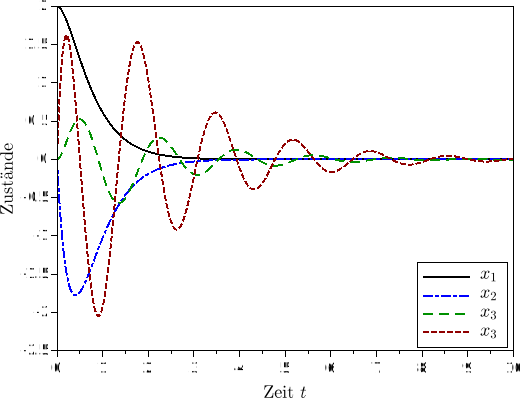
\includegraphics[width=0.85\textwidth]{Wagen-Pendel-Simulation}
\par\end{centering}
\caption{Simulationsergebnis des geregelten Wagen-Pendel-Systems\label{fig:Simulation-Wagen-Pendel-System}}
\end{figure}

\begin{remark}
\label{rem:regler-mit-AD}In der Rückführung~(\ref{eq:rueckfuehrung-stabilisierend-x})
können bei hohem relativen Grad umfangreiche symbolische Ausdrücke
auftreten. Bei der Implementierung des Reglers benötigt man nicht
zwangsläufig eine symbolische Darstellung, sondern nur eine Routine,
die den Ausdruck~(\ref{eq:rueckfuehrung-stabilisierend-x}) in jedem
Abtastschritt numerisch auswertet. Diese Funktionswertberechnung lässt
sich sehr effizient mit Hilfe des algorithmischen Differenzierens
implementieren~\cite{roebenack2000at,roebenack2005fgcs,roebenack2007mcmds}.
\end{remark}

\subsection{Nulldynamik}

Die \index{Nulldynamik}Nulldynamik~(\ref{eq:BINF-Nulldynamik})
wurde im vorangegangenen Abschnitt auf Basis der Byrnes-Isidori-Normalform~(\ref{eq:BINF-Matrixform})
definiert. Da die Berechnung dieser Normalform mitunter schwierig
ist, die Stabilitätsaussage der Nulldynamik (Minimalphasigkeit) aber
für die Stabilisierung des Gesamtsystems relevant ist, wird im Folgenden
ein alternativer Weg zur Berechnung der Nulldynamik angegeben~\cite[{Abschnitt~4.3}]{isidori3}. 

Die Nulldynamik erhält man aus der internen Dynamik in Gl.~(\ref{eq:BINF-Matrixform})
durch Nullsetzen des Zustands des ersten Teilsystems, also mit $\xi=0$.
Entsprechend der Definition der Koordinaten $\xi_{1}=h(x),\xi_{2}=L_{f}h(x),\ldots,\xi_{n}=L_{f}^{r-1}h(x)$
des ersten Teilsystems führt die Bedingung $\xi=0$ in Originalkoordinaten
auf die gleichungsdefinierte Untermannigfaltigkeit 
\begin{equation}
\mathcal{Z}^{*}=\left\{ x\in\mathcal{M}\subseteq\R^{n};\;h(x)=0,\;L_{f}h(x)=0,\;\ldots,\;L_{f}^{r-1}h(x)=0\right\} \label{eq:zwangsbedingung-nulldynamik-x}
\end{equation}
des Vektorraums~$\R^{n}$ der Dimension $n-r$. Mit $y=h(x)=0,\ldots,y^{(r-1)}=L_{f}^{r-1}h(x)=0$
ist zwar der Ausgang in einem Punkt Null, könnte aber durch ungünstige
Wahl des Eingangs aus dem Nullpunkt herausbewegt werden. Um $y(t)=0$
für alle $t\geq0$ sicherzustellen muss zusätzlich für die letzte
Differentialgleichung des ersten Teilsystems gelten: 
\[
\dot{\xi}_{r}=\alpha(\xi,\eta)+\beta(\xi,\eta)u\stackrel{!}{=}0.
\]
Daraus leitet sich unmittelbar die zusätzliche Bedingung 
\begin{equation}
u=-\frac{\alpha(\xi,\eta)}{\beta(\xi,\eta)}=-\frac{L_{f}^{r}h(x)}{L_{g}L_{f}^{r-1}h(x)}\label{eq:zwangsbedingung-nulldynamik-u}
\end{equation}
ab. Für das erste Teilsystem gilt somit 
\begin{equation}
\xi(0)=0\;\wedge\;\forall t\geq0:\;\dot{\xi}(t)=0\quad\Longrightarrow\quad\forall t\geq0:\;\xi(t)=0,\label{eq:nulldyn-TS1}
\end{equation}
woraus auch $y(t)=\xi_{1}(t)=0$ für alle $t\geq0$ folgt.

Mit der Zwangsbedingung~(\ref{eq:zwangsbedingung-nulldynamik-u})
kann man im zweiten Teilsystem der Eingangs-Ausgangs-Normalform~(\ref{eq:EANF-Matrixform})
den Eingangs~$u$ eliminieren
\[
\begin{array}{cll}
\dot{\eta} & = & q(\xi,\eta)+d(\xi,\eta)u\\
 & = & q(\xi,\eta)-d(\xi,\eta)\frac{\alpha(\xi,\eta)}{\beta(\xi,\eta)}\\
 & =: & \tilde{q}(\xi,\eta)
\end{array}
\]
und erhält damit die durch~$\tilde{q}$ beschriebene interne Dynamik
der Byrnes-Isidori-Normalform~(\ref{eq:BINF-Matrixform}). Zusammen
mit Gl.~(\ref{eq:nulldyn-TS1}) ergibt sich daraus die Nulldynamik\index{Nulldynamik}
\begin{equation}
\dot{\eta}=\tilde{q}(0,\eta).\label{eq:nulldyn-TS2}
\end{equation}

In den Originalkoordinaten geht das zu regelnde System~(\ref{eq:Ausgangssystem-fuer-BINF})
mit der Bedingung~(\ref{eq:zwangsbedingung-nulldynamik-u}) in das
autonome System 
\begin{equation}
\dot{x}=f(x)+g(x)u=f(x)-\frac{L_{f}^{r}h(x)}{L_{g}L_{f}^{r-1}h(x)}g(x)=:f^{*}(x)\label{eq:nulldynamik-f-stern}
\end{equation}
mit dem Vektorfeld~$f^{*}$ über. In den transformierten Koordinaten
entspricht dieses Vektorfeld der Nulldynamik~(\ref{eq:nulldyn-TS2}).
Zusammen mit~(\ref{eq:nulldyn-TS1}) ist die Nulldynamik (bezogen
auf den gesamten Zustandsraum $\R^{n}\cong\R^{r}\times\R^{n-r}$ bzw.
eine offenen Teilmenge davon) des Systems~(\ref{eq:EANF-Matrixform})
invariant bezüglich des durch $\xi=0$ definierten Teilraums $(\xi,\eta)\in0\times\R^{n-r}$.
In den Originalkoordinaten entspricht dieser Teilraum der in Gl.~(\ref{eq:zwangsbedingung-nulldynamik-x})
definierten Untermannigfaltigkeit~$\mathcal{Z}^{*}$ (siehe Abb.~\ref{fig:Nulldynamik}).

\begin{figure}
\begin{centering}
\resizebox{0.85\textwidth}{!}{\input{Nulldynamik.pdftex_t}}
\par\end{centering}
\caption{Darstellung der Nulldynamik\index{Nulldynamik} als Vektorfeld~$f^{*}$
auf der Untermannigfaltigkeit~$\mathcal{Z}^{*}$\label{fig:Nulldynamik}}

\end{figure}

Der Zusammenhang zwischen der Untermannigfaltigkeit~$\mathcal{Z}^{*}$
und dem Vektorfeld~$f^{*}$ wird zunächst an einem rein mathematischen
Beispiel illustriert. Der Stabilitätsaspekt spielt dabei keine Rolle,
da das System nicht in einer Ruhelage betrachtet wird.
\begin{example}
\label{exa:nulldynamik-fstar}Das auf $\mathcal{M}=\R^{2}$ definierte
System
\[
\begin{array}{lcl}
\dot{x}_{1} & = & -x_{2}+x_{1}(1-x1^{2}-x_{2}^{2})+x_{1}u\\
\dot{x}_{2} & = & \phantom{-}x_{1}+x_{2}(1-x1^{2}-x_{2}^{2})+x_{2}u\\
y & = & x_{1}^{2}+x_{2}^{2}-1
\end{array}
\]
hat die Form~(\ref{eq:Ausgangssystem-fuer-BINF}) und wegen $L_{g}h(x)=2(x_{1}^{2}+x_{2}^{2})$
den relativen Grad $r=1$. Die Menge $\mathcal{Z}^{*}=\{x\in\R^{2};\;h(x)=x_{1}^{2}+x_{2}^{2}-1=0\}$
nach Gl.~(\ref{eq:zwangsbedingung-nulldynamik-x}) ist der Einheitskreis.
Die Nulldynamik wird durch die Abbildung $f^{*}(x)=-x_{2}\tfrac{\partial}{\partial x_{1}}+x_{1}\tfrac{\partial}{\partial x_{2}}$
nach Gl.~(\ref{eq:nulldynamik-f-stern}) beschrieben. Abb.~\ref{fig:nulldynamik-fstar}
verdeutlicht, dass $f^{*}:\mathcal{Z}^{*}\to\R^{2}$ tangential zu~$\mathcal{Z}^{*}$
liegt, also wirklich ein Vektorfeld ist. Die Nulldynamik entspricht
offensichtlich einer kontinuierlichen Zunahme des Winkels in der $(x_{1},x_{2})$-Ebene.
Das lässt sich durch Berechnung der Byrnes-Isidori-Normalform
\[
\begin{array}{lcl}
\dot{\xi} & = & -2\xi(\xi+1)+2(\xi+1)u\\
\dot{\eta} & = & 1\\
y & = & \xi
\end{array}
\]
verifizieren, wobei für die Hintransformation $\xi=h(x)=x_{1}^{2}+x_{2}^{2}-1$,
$\eta=\arctan(x_{2},x_{1})$ und für die Rücktransformation $x_{1}=\sqrt{\xi+1}\,\cos\eta$,
$x_{2}=\sqrt{\xi+1}\,\sin\eta$ verwendet werden.\footnote{Der Arkustangens $\arctan(x_{2},x_{1})$ mit zwei Argumenten ermöglicht
die Ermittlung des Winkels für alle vier Quadranten (mit Ausnahme
des Nullpunkts). Im ersten Quadranten stimmt diese Funktion mit $\arctan(x_{2}/x_{1})$
überein.}
\end{example}
\begin{figure}
\begin{centering}
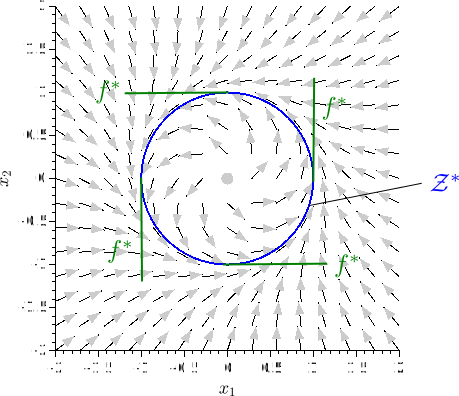
\includegraphics[width=0.65\textwidth]{nulldynamik_fstar}
\par\end{centering}
\caption{Phasen\-ebene zu Beispiel~\ref{exa:nulldynamik-fstar}: Vektorfeld
$f:\mathcal{M}\to\R^{2}$, Unter\-mannig\-faltig\-keit~$\mathcal{Z}^{*}$,
Vektor\-feld $f^{*}:\mathcal{Z}^{*}\to\R^{2}$ \label{fig:nulldynamik-fstar}}
\end{figure}

Bei den nächsten Beispielen wurde die Nulldynamik bereits über die
Byrnes-Isidori-Normalform berechnet. Die nachfolgenden Überlegungen
sind als Kontrollrechnung zu verstehen.

\begin{example}
\label{exa:mobiler-roboter-nulldynamik2}Für das Modell~(\ref{eq:roboter-rg-dgl})
des mobilen Roboters aus Beispiel~\ref{exa:Roboter-rel-grad} mit
dem Ausgang aus Beispiel~\ref{exa:Roboter-geregelt1} wurde der relative
Grad $r=2$ ermittelt. Zur Berechnung der Nulldynamik setzt man die
ersten $r=2$ Lie-Ableitungen (siehe Gl.~(\ref{eq:Roboter-BI-NF-hin1})
aus Beispiel~\ref{exa:Roboter-BI-NF}) zu Null, d.\,h. $x_{1}=0$
und $\sin x_{3}=0$. Wegen $L_{f}^{2}h(x)\equiv0$ vereinfacht sich
die Bedingung~(\ref{eq:zwangsbedingung-nulldynamik-u}) zu $u=0$.
Aus Gl.~(\ref{eq:roboter-rg-dgl}) erhält man damit folgendes autonomes
System: 
\[
\begin{array}{lclcl}
\dot{x}_{1} & = & 0\\
\dot{x}_{2} & = & \cos(\arcsin(0)) & = & \pm1\\
\dot{x}_{3} & = & 0
\end{array}
\]
Die resultierende Nullynamik $\dot{x}_{2}=\pm1$ beschreibt eine Bewegung
des Roboters parallel zur $x_{2}$-Achse. Die zwei Lösungen ergeben
sich entsprechend der Orientierung des Roboters, d.\,h. aus der Koordinate~$x_{3}$.
Für $x_{3}\in(-\pi/2,+\pi/2)$ erhält man in Übereinstimmung mit den
Beispielen~\ref{exa:Roboter-BI-NF} bzw.~\ref{exa:mobiler-roboter-nulldynamik1}
die Nulldynamik $\dot{x}_{2}=1$.
\end{example}

\begin{example}
\label{exa:wagen-pendel-system-nulldynamik2}Man betrachte das Wagen-Pendel-System
aus Beispiel~\ref{exa:Wagen-Pendel-partielle-Linearisierung}. Die
Bedingung~(\ref{eq:zwangsbedingung-nulldynamik-u}) erfüllt man im
partiell linearisierten System durch $v=0$. Damit geht Gl.~(\ref{eq:wagen-pendel-kollokiert-linearisiert})
in das System 
\begin{equation}
\begin{array}{lcl}
\dot{x}_{1} & = & 0\\
\dot{x}_{2} & = & 0\\
\dot{x}_{3} & = & x_{4}\\
\dot{x}_{4} & = & -\frac{d_{2}}{\ell^{2}m_{2}}x_{4}-\frac{g}{\ell}\sin x_{3}
\end{array}\label{eq:wagen-pendel-nulldynamik2}
\end{equation}
über. Die letzten zwei Differentialgleichungen stimmen mit der in
Beispiel~\ref{exa:wagen-pendel-system-nulldynamik1} berechneten
Nulldynamik überein.
\end{example}

\begin{remark}
\label{rem:Nulldynamik-Nullstellen-Uebertragungsfunktion}Die Nulldynamik
spiegelt sich bei einem linearen System auch in der Übertragungsfunktion
wider. Man betrachte das geregelte System~(\ref{eq:BINF-Stabilisiert})
mit der Systemmatrix $A_{11}:=A-bk^{T}$ des ersten Teilsystems~(\ref{eq:BINF-Stabilisiert1})
und einem linearen zweiten Teilsystem~(\ref{eq:BINF-Stabilisiert2}),
welches durch $q(\xi,\eta)=A_{21}\xi+A_{22}\eta$ mit $A_{21}\in\R^{(n-r)\times r}$
und $A_{22}\in\R^{(n-r)\times(n-r)}$ gegeben sei. Das Gesamtsystem
lautet dann 
\begin{equation}
\begin{array}{ccl}
\left(\begin{array}{c}
\dot{\xi}\\
\dot{\eta}
\end{array}\right) & = & \overbrace{\left(\begin{array}{cc}
A_{11} & 0\\
A_{21} & A_{22}
\end{array}\right)}^{{\displaystyle \bar{A}}}\left(\begin{array}{l}
\xi\\
\eta
\end{array}\right)+\overbrace{\left(\begin{array}{l}
b\\
0
\end{array}\right)}^{{\displaystyle \bar{b}}}u\\
y & = & \underbrace{\left(\begin{array}{cc}
c^{T} & 0\end{array}\right)}_{{\displaystyle \bar{c}^{T}}}\left(\begin{array}{l}
\xi\\
\eta
\end{array}\right).
\end{array}\label{eq:rel-grad-lineares-Gesamtsystem-ND}
\end{equation}
Die Übertragungsfunktion kann einererseits in der Form 
\begin{eqnarray}
G(s) & = & \frac{b_{n-r}s^{n-r}+\cdots+b_{1}s+b_{0}}{\det\left(sI_{n}-\bar{A}\right)}\nonumber \\
 & = & \frac{b_{n-r}s^{n-r}+\cdots+b_{1}s+b_{0}}{\det\left(sI_{r}-A_{11}\right)\cdot\det\left(sI_{n-r}-A_{22}\right)}\label{eq:rel-grad-UF1}
\end{eqnarray}
angesetzt werden. Der Nenner besteht aus dem charakteristischen Polynom
der Systemmatrix~$\bar{A}$. Wegen der Block\-dreiecks\-struktur
von~$\bar{A}$ zerfällt das charakteristische Polynom in das Produkt
der charakteristischen Polynome der Matrizen~$A_{11}$ und~$A_{22}$.
Bei einem relativen Grad~$r$ und einem Nennerpolynom vom Grad~$n$
weist das Zählerpolynom den Grad $n-r$ auf (siehe Anmerkung~\ref{rem:rel-grad-Uebertragungsfunktion}).
Andererseits kann man die Übertragungsfunktion unter Beachtung der
Block\-dreiecks\-struktur von~$\bar{A}$ direkt ausgerechnet werden:
\begin{eqnarray}
G(s) & = & \bar{c}^{T}\left(sI_{n}-\bar{A}\right)^{-1}\bar{b}\nonumber \\
 & = & \left(\begin{array}{cc}
c^{T} & 0\end{array}\right)\left(\begin{array}{cc}
sI_{r}-A_{11} & 0\\
-A_{21} & sI_{n-r}-A_{22}
\end{array}\right)^{-1}\left(\begin{array}{l}
b\\
0
\end{array}\right)\nonumber \\
 & = & \left(\begin{array}{cc}
c^{T} & 0\end{array}\right)\left(\begin{array}{cc}
\left(sI_{r}-A_{11}\right)^{-1} & 0\\
* & \left(sI_{n-r}-A_{22}\right)^{-1}
\end{array}\right)\left(\begin{array}{l}
b\\
0
\end{array}\right)\nonumber \\
 & = & c^{T}\left(sI_{r}-A_{11}\right)^{-1}b\nonumber \\
 & = & \frac{c^{T}\adj\left(sI_{r}-A_{11}\right)\,b}{\det\left(sI_{r}-A_{11}\right)}.\label{eq:rel-grad-UF2}
\end{eqnarray}
Das Zählerpolynom wird mit der Matrix der Adjunkten bzw. Kofaktoren
gebildet~\cite{reinschke88}. Das Nennerpolynom ist das charakteristische
Polynom der Matrix~$A_{11}$ und hat damit den Grad~$r$. Nach Anmerkung~\ref{rem:rel-grad-Uebertragungsfunktion}
muss auch bei Gl.~(\ref{eq:rel-grad-UF2}) zwischen Zähler- und Nennergrad
die Differenz~$r$ auftreten, so dass der Nenner in Gl.~(\ref{eq:rel-grad-UF2})
konstant sein muss. Ohne Einschränkungen sei der Nenner Eins. Die
unterschiedlichen Nennergrade von~(\ref{eq:rel-grad-UF1}) und~(\ref{eq:rel-grad-UF2})
lassen sich dadurch erklären, dass das zweite Teil\-system nicht
beobachtbar ist und daher in der Übertragungsfunktion zwischen Zähler
und Nenner gekürzt werden kann (siehe auch Beispiel~\ref{exa:Lineares-System-r-infty}).
Der Vergleich zwischen~(\ref{eq:rel-grad-UF1}) und~(\ref{eq:rel-grad-UF2})
führt damit unmittelbar auf
\[
b_{n-r}s^{n-r}+\cdots+b_{1}s+b_{0}=\det\left(sI_{n-r}-A_{22}\right),
\]
so dass das Zählerpolynom von~(\ref{eq:rel-grad-UF1}) das charakteristische
Polynom der Matrix~$A_{22}$ ist. Die Eigenwerte der Systemmatrix
$A_{22}$ der Nulldynamik von~(\ref{eq:rel-grad-lineares-Gesamtsystem-ND})
fallen folglich mit den Nullstellen der Übertragungsfunktion~(\ref{eq:rel-grad-UF1})
zusammen.
\end{remark}

Bei komplizierten Systemen kann man versuchen, die Stabilität der
Nulldynamik durch Taylor-Linearisierung in den Originalkoordinaten
zu untersuchen. Die zur Berechnung der Nulldynamik angegebene Bedingung~(\ref{eq:zwangsbedingung-nulldynamik-u})
kann man dabei auch als eine Vorgabe von $r$ Eigenwerten bei Null
verstehen. Nach einer Taylor-Linearisierung des resultierenden Systems~(\ref{eq:nulldynamik-f-stern})
in der betreffenden Ruhelage sind die verbleibenden $n-r$ Eigenwerte
der Jacobi\-matrix der Nulldynamik zuzuordnen. Besitzen alle Eigenwerte
der Nulldynamik einen nichtverschwindenden Realteil, so liegt für
die Nulldynamik eine \emph{hyperbolische Ruhelage}\index{Ruhelage!hyperbolische}
vor. Nach dem Satz von Hartman-Grobman\index{Satz!von Hartman-Grobman}
ist bei einer hyperbolischen Ruhelage das nichtlineare System in einer
Umgebung der betreffenden Ruhelage topologisch konjugiert\index{topologisch konjugiert}
bzw. zustandsäquivalent\index{zustandsäquivalent} zu seiner Taylor-Linearisierung~\cite{guckenheimer83,arrowsmith90}.
Besitzen alle der Nulldynamik zugeordneten $n-r$ Eigenwerte einen
negativen Realteil, so ist die Ruhelage (lokal) asymptotisch stabil.
Gibt es einen Eigenwert mit positivem Realteil, dann ist die Ruhelage
instabil. Weist die Linearisierung der Nulldynamik dagegen einen Eigenwert
mit Realteil Null auf, dann ist die Ruhelage nicht hyperbolisch. (Bezogen
auf die Linearisierung des Gesamtsystems bedeutet das, dass es mehr
als $r$ Eigenwerte bei Null gibt oder ein rein imaginäres Eigenwertpaar
auftritt.) Selbst wenn alle anderen Eigenwerte einen negativen Realteil
besitzen ist in diesem Fall keine Stabilitätsaussage auf Basis der
Linearisierung möglich. Die Stabilität der Ruhelage könnte man dann
mit Hilfe des Satzes über die Zentrumsmannigfaltigkeit\index{Satz!über die Zentrumsmannigfaltigkeit}
untersuchen~\cite{guckenheimer83,arrowsmith90}.
\begin{example}
Die Taylor-Linearisierung von~(\ref{eq:wagen-pendel-nulldynamik2})
im Ursprung $x=0$ führt auf das System
\[
\left(\begin{array}{c}
\dot{x}_{1}\\
\dot{x}_{2}\\
\dot{x}_{3}\\
\dot{x}_{4}
\end{array}\right)=\left(\begin{array}{cccc}
0 & 0 & 0 & 0\\
0 & 0 & 0 & 0\\
0 & 0 & 0 & 1\\
0 & 0 & -\frac{g}{l} & -\frac{d_{2}}{l^{2}m_{2}}
\end{array}\right)\left(\begin{array}{l}
x_{1}\\
x_{2}\\
x_{3}\\
x_{4}
\end{array}\right)
\]
mit dem charakteristischen Polynom 
\[
s^{2}\cdot\left(s^{2}+\frac{d_{2}}{l^{2}m_{2}}s+\frac{g}{l}\right).
\]
Die doppelte Nullstelle bei $s=0$ resultiert unmittelbar aus der
Bedingung~(\ref{eq:nulldyn-TS1}). Das verbleibende Polynom zweiter
Ordnung ist nach der Stodola-Bedingung (siehe~\cite{reinschke2014buch})
für die relevanten Parameterwerte $g,l,d_{2},m_{2}>0$ ein Hurwitz-Polynom.
Alle Eigenwerte der Nulldynamik besitzen somit einen negativen Realteil.
Die Ruhelage $\eta=0$ ist daher (lokal) asymptotisch stabil. 
\end{example}

\subsection{Äquivalenz von Systemen und globale Stabilisierung\label{subsec:Equivalenz-globale-Stab}}

Setzt man die linearisierende Rückführung~(\ref{eq:rueckfuehrung-linearisierend})
in die Systemgleichungen~(\ref{fig:Ausgangssystem-fuer-BINF}) ein,
so erhält man das System 
\begin{equation}
\begin{array}{lcl}
\dot{x} & = & f(x)+g(x)u\\
 & = & f(x)+g(x)\frac{1}{L_{g}L_{f}^{r-1}h(x)}\left(v-L_{f}^{r}h(x)\right)\\
 & = & \underbrace{f(x)-\frac{L_{f}^{r}h(x)}{L_{g}L_{f}^{r-1}h(x)}g(x)}_{{\displaystyle f^{*}(x)}}+\underbrace{\frac{1}{L_{g}L_{f}^{r-1}h(x)}g(x)}_{{\displaystyle g^{*}(x)}}\,v
\end{array}\label{eq:linearisiertes-System-in-x}
\end{equation}
mit den Vektorfeldern~$f^{*}$ und~$g^{*}$. Das System~(\ref{eq:linearisiertes-System-in-x})
wird in einer Umgebung des Punktes~$p$ durch den (lokalen) Diffeomorphismus~$\Phi$
in das System~(\ref{eq:BINF-Linearisiert}) überführt. Diese Systeme
sind dann \emph{zustands\-äquivalent}\index{zustandsäquivalent}
(engl. \emph{state equivalent}), siehe~\cite{dayawansa1985}. (Damit
wird der in Kapitel~\ref{chap:Diff-Geo} eingeführte Begriff der
Zustands\-äquivalenz auf Systeme mit Eingang erweitert.) Ist die
Zustands\-transformation~$\Phi$ ein globaler Diffeomorphismus,
so nennt man die Systeme \emph{global zustands\-äquivalent}. Im Allgemeinen
sind die Existenzbedingungen für eine globale Transformation sehr
restriktiv. Für den Fall, dass man die Transformation explizit ausrechnen
kann und $\mathcal{M}=\R^{n}$ gilt, sind in~\cite{wu72} überprüfbare
Bedingungen angegeben.

Bei einem im Punkt $p\in\mathcal{M}$ wohldefinierten relativen Grad~$r$
ist das System~(\ref{fig:Ausgangssystem-fuer-BINF}) in einer Umgebung
von~$p$ zustandsäquivalent zu einem System der Bynres-Isidori-Normalform~(\ref{eq:BINF-Matrixform}).
Eine notwendige Bedingung für eine globale Zustandsäquivalenz ist
ein konstanter relativer Grad:
\begin{definition}
\label{def:gleichmaessiger-relativer-grad}System~(\ref{fig:Ausgangssystem-fuer-BINF})
hat einen \emph{gleichmäßigen relativen Grad}\index{relativer Grad!gleichmäßiger}
(engl. \emph{uniform relative degree}), falls es den relativen Grad~$r$
nach Definition~\ref{def:relativer-Grad-SISO} für alle $p\in\mathcal{M}$
besitzt.
\end{definition}
Basierend auf \cite{byrnes91nf} und~\cite[Kapitel~9]{isidori3}
lässt sich folgende Existenzaussage treffen:
\begin{theorem}
\label{them:globale-BINF}Wir betrachten System~(\ref{fig:Ausgangssystem-fuer-BINF})
auf einer offenen und zusammenhängenden Menge $\mathcal{M}\subseteq\R^{n}$.
Das System habe einen gleichmäßigen relativen Grad~$r$. Ferner gelte~(\ref{eq:Ruhelage-x})
und~(\ref{eq:Ruhelage-y}). Sind die Vektorfelder 
\begin{equation}
g^{*},\ad_{-f^{*}}g^{*},\ldots,\ad_{-f^{*}}^{r-1}g^{*}:\mathcal{M}\to\R^{n}\label{eq:VF-ad-g-tilde}
\end{equation}
vollständig\index{Vektorfeld!vollständiges}\footnote{Ein Vektorfeld heißt \textit{vollständig}, wenn es einen globalen
Fluss besitzt (vgl. Abschnitt~\ref{sec:Vektorfelder-und-Fluesse}).}, so ist das System~(\ref{eq:linearisiertes-System-in-x}) global
zustandsäquivalent zu einem System der Form~(\ref{eq:BINF-Linearisiert}).
\end{theorem}
Mit Gln.~(\ref{eq:Ruhelage-x}) und~(\ref{eq:Ruhelage-y}) ist die
Menge~$\mathcal{Z}^{*}$ nicht leer. Dann ist sie auch zusammenhängend.
Die Koordinatentransformation wird über die Flussverkettung der Vektorfelder~(\ref{eq:VF-ad-g-tilde})
konstruiert. Allerdings ist es in der Regel nicht leicht zu überprüfen,
ob ein gegebenes Vektorfeld vollständig ist. Eine Möglichkeit dazu
bietet der Satz von Wintner und Conti~\cite{reitmann96}.

\medskip{}

Der Übergang vom gegebenen System~(\ref{fig:Ausgangssystem-fuer-BINF})
zu der Form~(\ref{eq:linearisiertes-System-in-x}) erfolgt durch
die Rück\-führung~(\ref{eq:rueckfuehrung-linearisierend}). Zwei
Systeme heißen \emph{äquivalent unter statischer Zustandsrückführung},
(kurz \emph{rück\-führ\-äquivalent}\index{rückführäquivalent}
(engl. \emph{feed\-back equivalent}), wenn es eine statische Zustandsrückführung
gibt, so dass die Systeme zustandsäquivalent sind. Die Systeme heißen
\emph{global rück\-führ\-äquivalent}, falls die betrachteten Systeme
unter einer auf ganz $\mathcal{M}$ definierten Zustandsrückführung
global zustands\-äquivalent sind. Durch die Kombination aus Zustandstransformation
und Zustandsrückführung kann man die Systeme ineinander überführen.
In diesem Sinne sind die Systeme~(\ref{fig:Ausgangssystem-fuer-BINF})
und~(\ref{eq:linearisiertes-System-in-x}) rückführäquivalent, wobei
die Rückführung durch Gl.~(\ref{eq:rueckfuehrung-linearisierend})
gegeben ist. Das folgende Diagramm illustriert die Äquivalenzen einiger
der bisher betrachteten Systeme:

\[
\begin{tikzcd}
\text{(System~\ref{eq:Ausgangssystem-fuer-BINF})} 
\arrow[leftrightarrow]{rr}[above]{\stackrel{\textstyle\text{zustands-}}{\textstyle\text{äquivalent}}} 
\arrow[leftrightarrow]{d}[left]{\stackrel{\textstyle\text{rückführ-}}{\textstyle\text{äquivalent}}\quad} \arrow[rrd, leftrightarrow] 
& {} & \text{System~(\ref{eq:BINF-Matrixform})} 
\arrow[leftrightarrow]{d}[right]{\quad\stackrel{\textstyle\text{rückführ-}}{\textstyle\text{äquivalent}}}
\arrow[lld, leftrightarrow, crossing over]\\ 
\text{System~(\ref{eq:linearisiertes-System-in-x})} 
\arrow[leftrightarrow]{rr}[below]{\stackrel{\textstyle\text{zustands-}}{\textstyle\text{äquivalent}}} 
& {} & \text{System~(\ref{eq:BINF-Linearisiert})}
\end{tikzcd}
\]

Die lokale Stabilisierung des Systems~(\ref{fig:Ausgangssystem-fuer-BINF})
mittels Eingangs-Ausgangs-Linearisierung setzt nach Satz~\ref{thm:Stabilisierung-EA-lokal}
die lokale asymptotische Stabilität der Nulldynamik~(\ref{eq:BINF-Nulldynamik})
voraus. Für eine globale Stabilisierung nach dem gleichen Schema (also
mit einer linearen Rückführung im eingangs-ausgangs-linearisierten
ersten Teilsystem) ist selbst die globale asymptotische Stabilität
der Nulldynamik~(\ref{eq:BINF-Nulldynamik}) nicht hinreichend~\cite{sussmann1990}.
Das nachfolgende Beispiel wurde~\cite[Example~{4.2}]{sepulchre97}
entnommen:

\begin{example}
\label{exa:keine-globale-stabiliserung-mit-linearer-rueckf}Das System
\[
\begin{array}{lcl}
\dot{\xi} & = & u\\
\dot{\eta} & = & -\eta+\eta^{2}\xi
\end{array}
\]
liegt bereits in der partiell linearisierten Form~(\ref{eq:BINF-Linearisiert})
vor. Die Rückführung $u=-k\xi$ mit $k>0$ sichert die globale asymptotische
Stabilität der Ruhelage $\xi=0$ des ersten Teilsystems. Die Nulldynamik
$\dot{\eta}=-\eta$ ist ebenfalls global asymptotisch stabil. Damit
ist die Ruhelage $(\xi,\eta)=(0,0)$ lokal asmptotisch stabil, aber
nicht global: Der Anfangswert $\xi(0)=1$ liefert für das rückgeführte
erste Teilsystem die Lösung $\xi(t)=\e^{-t}$. Setzt man diese Lösung
in das zweite Teilsystem ein, so ergibt sich für den Anfangswert $\eta(0)=p$
die Lösung
\[
\eta(t)=\frac{(k+1)p\e^{-t}}{p\e^{-(k+1)t}-p+k+1}.
\]
Geht man von $p>0$ aus, so hat die Lösung für $p>k+1$ eine Polstelle
und damit eine endliche Fluchtzeit (vgl. auch Beispiel~\ref{exa:EndlicheFluchtzeit}).

Ein aussagekräftiges Konzept für eine globale Stabilitätsaussage ist
die \emph{Eingangs-Zustands-Stabilität} (engl. \emph{input-state stability},
kurz \emph{ISS}), siehe~\cite{sontag1995ejc,sontag2000} und Anhang~\ref{sec:Stabilitaet-erregter-Systeme}.
Wir nennen ein System \emph{stark minimalphasig}\index{minimalphasig!stark}
(engl. \emph{strongly minimum phase}), wenn die interne Dynamik nach
Gl.~(\ref{eq:BINF-Stabilisiert2}) eingangs-zustands-stabil\index{eingangs-zustands-stabil}
bezüglich~$\xi$ (als Eingang) ist~\cite{liberzon2000,isidori2013ejc}.
\end{example}
\begin{theorem}
\label{thm:Stabilisierung-EA-global}Das System~(\ref{eq:Ausgangssystem-fuer-BINF})
habe den Arbeitspunkt $p\in\mathcal{M}$ (für $u=0$) und den gleichmäßigen
relativen Grad $r<n$. Zusätzlich sei das System global rück\-führ\-äquivalent
zu der Form~(\ref{eq:BINF-Stabilisiert}) mit der Ruhelage $(\xi,\eta)=(0,0)$.
Die Reglerverstärkung $k\in\R^{r}$ sei so gewählt, dass das charakteristische
Polynom~(\ref{eq:TS1-charakteristisches-Polynom}) ein Hurwitz-Polynom
ist. Ist das System stark minimalphasig, dann ist die Ruhelage~$p$
des resultierenden Systems global asymptotisch stabil.
\end{theorem}
\begin{svmultproof2}
Durch die Wahl der Reglerverstärkung~$k$ besitzt die Matrix $A-bk^{T}$
nur Eigenwerte mit negativem Realteil. Die Ljapunov-Funktion~$V_{1}$
für das erste Teil\-system~(\ref{eq:BINF-Stabilisiert1}) lässt
sich daher wie im Beweis von Satz~(\ref{thm:Stabilisierung-EA-lokal})
über die Ljapunov-Gleichung~(\ref{eq:TS1-Lyap-Gleichung}) konstruieren.
Außerdem wurde angenommen, dass das zweite Teilsystem~(\ref{eq:BINF-Stabilisiert2})
eingangs-zustands-stabil bezüglich~$\xi$ ist. Damit liegt eine Kaskadenstruktur
entsprechend Abb.~\ref{fig:Kaskadenstruktur-EA-Linearisierung} vor.
Entsprechend Anhang~\ref{sec:Stabilitaet-erregter-Systeme} ist damit
die Ruhelage $(\xi,\eta)=(0,0)$ global asymptotisch stabil.
\end{svmultproof2}

Erweitert man die Rückführung~(\ref{eq:rueckfuehrung-stabilisierend})
wie in Gl.~(\ref{eq:regler4-linearisierung-stabilisierung-sollwert-y})
mit um einen Eintrag hinsichtlich der Führungsgröße~$w$, so erhält
man für das Eingangs-Ausgangs-Verhalten des ersten Teilsystems
\begin{equation}
\begin{array}{lcl}
\dot{\xi} & = & \left(A-bk^{T}\right)\xi+a_{0}bw\\
y & = & c^{T}\xi
\end{array}\label{eq:TS1-stabilisiert-mit-Fuerungsgroesse}
\end{equation}
die Übertragungsfunktion~(\ref{eq:UF-WY}). Die Rückführung kann
in Originalkoordinaten durch Gl.~(\ref{eq:regler4-linearisierung-stabilisierung-sollwert-x})
ausgedrückt werden. Für den Fall eines sich zeitlich veränderlichen
Verlauf der Führungsgröße~$w$ liegt keine Ruhelage vor. Daher ist
auch die asymptotische Stabilität nicht sehr hilfreich. Im Falle eines
eingangs-zustands-stabilen Systems hat man die Gewissheit, dass bei
einem beschränkten Eingangs- bzw. Führungssignal~$w$ der Zustand
ebenfalls beschränkt bleibt.
\begin{theorem}
\label{thm:Stabilisierung-EA-global-fuehrungssignal}Das System~(\ref{eq:Ausgangssystem-fuer-BINF})
habe den Arbeitspunkt $p\in\mathcal{M}$ (für $u=0$) und den gleichmäßigen
relativen Grad $r<n$. Zusätzlich sei das System global rück\-führ\-äquivalent
zu der Form~(\ref{eq:TS1-stabilisiert-mit-Fuerungsgroesse}), (\ref{eq:BINF-Stabilisiert2})
mit der Ruhelage $(\xi,\eta)=(0,0)$. Die Reglerverstärkung $k\in\R^{r}$
sei so gewählt, dass das charakteristische Polynom~(\ref{eq:TS1-charakteristisches-Polynom})
ein Hurwitz-Polynom ist. Ist das System stark minimalphasig, dann
ist das resultierende Gesamtsystem eingangs-zustands-stabil.
\end{theorem}
\begin{svmultproof2}
Laut Annahme hat die Matrix $A-bk^{T}$ nur Eigenwerte mit negativem
Realteil. Das lineare Teilsystem~(\ref{eq:TS1-stabilisiert-mit-Fuerungsgroesse})
ist daher eingangs-zustands-stabil. Das zweite Teilsystem~(\ref{eq:BINF-Stabilisiert2})
ist ebenfalls eingangs-zustands-stabil. Damit ist auch das Gesamtsystem
eingangs-zustands-stabil (siehe Anhang~\ref{sec:Stabilitaet-erregter-Systeme}).
\end{svmultproof2}

In den Sätzen~\ref{thm:Stabilisierung-EA-global} und~\ref{thm:Stabilisierung-EA-global-fuehrungssignal}
wurde die Annahme der Minimalphasigkeit, d.\,h. der asymptotischen
Stabilität der Nulldynamik~(\ref{eq:BINF-Nulldynamik}), durch die
Eigenschaft der Eingangs-Zustands-Stabilität ersetzt. Andere Möglichkeiten
zur Charakterisierung der Stabilität der internen Dynamik sind beispielsweise
in~\cite{krichman1999,liberzon2000} angegeben.

\section{Exakte Eingangs-Zustands-Linearisierung\label{sec:Exakte-Eingangs-Zustands-Linearisierung}}

\subsection{Problemformulierung\label{subsec:EZ-Linearisierung-Problemformulierung}}

Bei der Eingangs-Ausgangs-Linearisierung eines Systems~(\ref{eq:Ausgangssystem-fuer-BINF})
mit relativem Grad~$r$ erhält man ein lineares erstes Teilsystem
der Dimension~$r$. Für $r<n$ verbleibt im Gesamtsystem ein nicht
zu beeinflussendes und in der Regel nichtlineares zweites Teilsystem
des Dimension $n-r$. Es stellt sich folgende Frage: Wann kann ein
System 
\begin{equation}
\dot{x}=f(x)+g(x)u\label{eq:system-fuer-eingangs-zustands-lin}
\end{equation}
mit glatten Vektorfeldern $f,g:\mathcal{M}\to\R^{n}$ in einer Umgebung
eines Punktes $p\in\mathcal{M}$ \textit{vollständig} in ein lineares
steuerbares System überführt werden, so dass kein zweites Teil\-system
übrigbleibt? Dieses Problem der \emph{(exakten) Eingangs-Zustands-Linearisierung}\index{Linearisierung!Eingangs-Zustands-}
ist lösbar, wenn es eine Ausgangsabbildung $h:\mathcal{M}\to\R$ gibt
(d.\,h. ein Skalarfeld), so dass das System~(\ref{eq:system-fuer-eingangs-zustands-lin})
den relativen Grad~$n$ besitzt. Ein solches System nennt man \emph{eingangs-zustands-linearisierbar}. 

Bei vielen Systemen ist aus Sicht des Anwenders bereits ein Ausgang
als Regel- oder Messgröße vorgegeben, für den das System im Sinne
der Eingangs-Ausgangs-Linearisierung einen (festen) relativen Grad~$r$
besitzt. Bei der Eingangs-Zustands-Linearisierung sucht man einen
(zunächst als reine Hilfsgröße eingeführten) Ausgang mit relativem
Grad~$n$, auf dessen Basis eine Zustandsrückführung entworfen wird.

Bei einem eingangs-zustands-linearisierbaren System gehen sowohl die
Eingangs-Ausgangs-Normalform~(\ref{eq:EA-Form-komponentenweise})
als auch die Byrnes-Isidori-Normaform~(\ref{eq:BINF-Komponentenweise})
in die \emph{Regelungsnormalform}\index{Regelungsnormalform}\index{Normalform!Regelungs-}
(engl. \emph{controller canonical form}) 
\begin{equation}
\begin{array}{lcl}
\dot{z}_{1} & = & z_{2}\\
 & \vdots\\
\dot{z}_{n-1} & = & z_{n}\\
\dot{z}_{n} & = & \alpha(z)+\beta(z)u\\
y & = & z_{1}
\end{array}\label{eq:Regelungsnormalform}
\end{equation}
 über (siehe Abb.~\ref{fig:regelungsnormalform} sowie~\cite{zeitz85,zeitz89}).
Entsprechend Gl.~(\ref{eq:alpha-beta-EA-NF}) ergeben sich die Skalarfelder~$\alpha$
und $\beta$ aus 
\begin{equation}
\begin{array}{lcl}
\alpha(z) & = & \left.L_{f}^{n}h(x)\right|_{x=\Phi^{-1}(z)}\\
\beta(z) & = & \left.L_{g}L_{f}^{n-1}h(x)\right|_{x=\Phi^{-1}(z)}
\end{array}\label{eq:alpha-beta-EZ-Regelungs-NF}
\end{equation}
mit $\beta(\Phi(p))\neq0$. Mit der Zustandsrückführung
\begin{equation}
u=\frac{1}{\beta(z)}\left(v-\alpha(z)\right)\label{eq:rueckfuehrung-EZ}
\end{equation}
erhält man aus dem (bedingt durch die Skalarfelder~$\alpha$ und
$\beta$ typischerweise nichtlinearen) System~(\ref{eq:Regelungsnormalform})
ein lineares steuerbares System in Brunovský-Normalform\index{Brunovský-Normalform}\index{Normalform!Brunovský-}~\cite{brunovsky70}
\begin{equation}
\left.\begin{array}{lcl}
\dot{z}_{1} & = & z_{2}\\
 & \vdots\\
\dot{z}_{n-1} & = & z_{n}\\
\dot{z}_{n} & = & v\\
y & = & z_{1}
\end{array}\right\} \quad\begin{array}{ccl}
\dot{x} & = & Ax+bv\\
y & = & c^{T}v
\end{array}\label{eq:Brunovsky-Normalform}
\end{equation}
mit der Matrix $A\in\R^{n\times n}$ und dem Vektor \textbf{$b\in\R^{n}$}
entspr. Gl.~(\ref{eq:Abc-Brunovsky}). Ein System~(\ref{eq:system-fuer-eingangs-zustands-lin})
ist genau dann eingangs-zustands-linearisierbar, wenn es zustands\-äquivalent
zu~(\ref{eq:Regelungsnormalform}) bzw. rück\-führ\-äquivalent
zu~(\ref{eq:Brunovsky-Normalform}) ist.

\begin{figure}
\begin{centering}
\resizebox{0.9\textwidth}{!}{\input{regelungsnormalform.pdftex_t}}
\par\end{centering}
\caption{Regelungsnormalform~(\ref{eq:Regelungsnormalform}) eines eingangsaffinen
Systems~(\ref{eq:Ausgangssystem-fuer-BINF})\label{fig:regelungsnormalform}}
\end{figure}


\subsection{Problemlösung über Distributionen\label{subsec:EZ-Linearisierung-Distributionen}}

System~(\ref{eq:system-fuer-eingangs-zustands-lin}) ist genau dann
in einem Punkt $p\in\mathcal{M}$ eingangs-zustands-linearisierbar,
wenn es eine Ausgangsabbbildung $h:\mathcal{M}\to\R$ (also ein Skalarfeld)
gibt, so dass das System in dem betreffenden Punkt den relativen Grad~$n$
besitzt. Nach der Definition des relativen Grades muss in diesem Fall
\begin{equation}
\begin{array}{rclll}
L_{g}L_{f}^{i}h(x) & = & 0 & \mbox{für} & 0\leq i\leq n-2,\\
L_{g}L_{f}^{n-1}h(p) & \neq & 0
\end{array}\label{eq:ex-ein-zu0}
\end{equation}
für alle~$x$ aus einer Umgebung von~$p$ gelten. Entsprechend Lemma~\ref{lem:Skalarprod-dLf-ad}
gilt daher auch 
\[
L_{\ad_{-f}^{i}g}L_{f}^{j}h=\left\langle \d L_{f}^{j}h,\ad_{-f}^{i}g\right\rangle =\left\{ \begin{array}{ccccc}
0 & \mbox{für} & i+j & < & n-1,\\
L_{g}L_{f}^{n-1}h & \mbox{für} & i+j & = & n-1.
\end{array}\right.
\]
Für $j=0$ erhält man 
\begin{eqnarray}
L_{\ad_{-f}^{i}g}h(x) & = & 0\quad\mbox{for}\quad0\leq i\leq n-2\label{eq:ex-ein-zu1}\\
L_{\ad_{-f}^{n-1}g}h(p) & \neq & 0.\label{eq:ex-ein-zu2}
\end{eqnarray}
Wegen $L_{\ad_{-f}^{i}g}h=\langle\d h,\ad_{-f}^{i}g\rangle$ kann
man die $n-1$ Gleichungen~(\ref{eq:ex-ein-zu1}) auch in der Form
\begin{equation}
\d h(x)\cdot\left(g(x),\ad_{-f}g(x),\ldots,\ad_{-f}^{n-2}g(x)\right)=\left(0,0,\ldots,0\right)\label{eq:ex-ein-zu-PDE}
\end{equation}
angeben. Damit erhält man eine (vektorwertige) partielle Differentialgleichung
erster Ordnung für die Unbekannte~$h$. Zur Untersuchung der Lösbarkeit
wird die Folge 
\begin{equation}
\Delta_{i}(x)=\spann\left\{ g(x),\ad_{-f}g(x),\ldots,\ad_{-f}^{i-1}g(x)\right\} \label{eq:Distributionen-Delta-i}
\end{equation}
von Distributionen\index{Distribution} definiert. Der nachfolgende
Satz gibt die genauen Existenzbedingungen für eine Ausgangsabbildung
mit vollem relativen Grad an~\cite{su1982}, \cite[Theorem~{4.2.3}]{isidori3}:
\begin{theorem}
\label{thm:Exakte-Eingangs-Zustands_Linearisierung}Das System~(\ref{eq:system-fuer-eingangs-zustands-lin})
besitzt im Punkt $p\in\mathcal{M}$ genau dann eine Ausgangsabbildung~$h$
mit relativem Grad~$n$, wenn gilt:
\begin{enumerate}
\item \label{enu:exakt-dim}$\dim\,\Delta_{n}(p)=n$ und
\item \label{enu:exakt-involutiv}$\Delta_{n-1}$ ist involutiv in einer
Umgebung von~$p$.\index{involutive Distribution}\index{Distribution!involutive}
\end{enumerate}
\end{theorem}
\begin{svmultproof2}
\hinreichend\ Das System~(\ref{eq:system-fuer-eingangs-zustands-lin})
habe im Punkt $p\in\mathcal{M}$ den relativen Grad~$n$ für eine
Ausgangsabbildung~$h$. Wegen Lemma~\ref{lem:Skalarprod-dLf-ad}
gilt
\begin{equation}
\begin{array}{l}
\left(\begin{array}{c}
\d h(p)\\
\d L_{f}h(p)\\
\vdots\\
\d L_{f}^{n-1}h(p)
\end{array}\right)\left(g(p),\ad_{-f}g(p),\ldots,\ad_{-f}^{n-1}g(p)\right)=\\
=\left(\begin{array}{cccc}
0 & \cdots & 0 & L_{g}L_{f}^{n-1}h(p)\\
\vdots & \qdots &  & *\\
0 &  & \qdots & \vdots\\
L_{g}L_{f}^{n-1}h(p) & * & \cdots & *
\end{array}\right).
\end{array}\label{eq:beweis-ez-linearisierbarkeit-unabh-VF}
\end{equation}
Daraus folgt $\dim\,\Delta_{n}(p)=n$. Außerdem folgt aus der linearen
Unabhängigkeit der Vektoren $g(p),\ldots,\ad_{-f}^{n-1}g(p)$ auch
$\dim\,\Delta_{n-1}=n-1$. Damit ist die Distribution $\Delta_{n-1}$
im Punkt~$p$ regulär. Aufgrund des relativen Grades~$n$ gilt~(\ref{eq:ex-ein-zu-PDE})
(siehe Vorbetrachtungen zum Satz), d.\,h. der Gradient $\d h$ spannt
den Annihilator von $\Delta_{n-1}$ auf. Nach dem Satz von Frobenius
(Satz~\ref{thm:Frobenius-lokal}) ist $\Delta_{n-1}$ involutiv.

\notwendig\ Laut Voraussetzung gilt $\dim\Delta_{n}(p)=n$, so dass
diese Distrubution den vollen Vektor\-raum~$\R^{n}$ aufspannt.
Aus Stetigkeitsgründen gilt dann auch $\dim\Delta_{n}(x)=n$ für eine
Umgebung von~$p$, so dass die Distribution~$\Delta_{n}$ im Punkt~$p$
regulär ist. Durch die Wegnahme des Vektorfeldes $\ad_{-f}^{n-1}g$
erhält man die reguläre Distribution~$\Delta_{n-1}$ mit $\dim\,\Delta_{n-1}=n-1$.
Außerdem wurde angenommen, dass $\Delta_{n-1}$ involutiv ist. Nach
dem Satz von Frobenius existiert ein Skalarfeld~$h$, dessen Gradient
die Vektorfelder von $\Delta_{n-1}$ annihiliert, d.\,h. 
\[
0=\left\langle \d h,\ad_{-f}^{i}g\right\rangle =L_{\ad_{-f}^{i}g}h\quad\mbox{für}\quad i=0,\ldots,n-2.
\]
 Damit ist Gl.~(\ref{eq:ex-ein-zu1}) erfüllt. Außerdem gilt~(\ref{eq:ex-ein-zu2}),
d.\,h. 
\begin{equation}
0\neq\left\langle \d h,\ad_{-f}^{n-1}g\right\rangle (p)=L_{\ad_{-f}^{n-1}g}h(p),\label{eq:beweis-ez-ungleichung}
\end{equation}
denn andernfalls würde $\d h$ den Annihilator von $n$ linear unabhängigen
Vektorfeldern aufspannen (Widerspruch zur Dimensionsformel~(\ref{eq:dimensionssatz-distr-annihilator})
aus Prop.~\ref{pro:Annihilator}). Wegen Gl.~(\ref{eq:ex-ein-zu1})
und~(\ref{eq:ex-ein-zu2}) hat das System~(\ref{eq:system-fuer-eingangs-zustands-lin})
mit dem Ausgang~$h$ den relativen Grad~$n$.
\end{svmultproof2}

\begin{remark}
\label{rem:Steuerbarkeitsmatrix}Die Bedingung~\ref{enu:exakt-dim}
von Satz~\ref{thm:Exakte-Eingangs-Zustands_Linearisierung} bedeutet,
dass die \emph{Steuerbarkeitsmatrix}\index{Steuerbarkeitsmatrix}\index{Matrix!Steuerbarkeits-}
bzw. \emph{Erreichbarkeitsmatrix}\index{Erreichbarkeitsmatrix}\index{Matrix!Erreichbarkeits-}
(engl. \emph{controllability matrix}, \emph{reachability matrix})
\begin{equation}
Q_{S}(x)=\left(g(x),\ad_{-f}g(x),\ldots,\ad_{-f}^{n-1}g(x)\right)\label{eq:Steuerbarkeitsmatrix-nichtlinear}
\end{equation}
im Punkt~$p$ regulär ist, d.\,h. $\rank\,Q_{S}(p)=n$. Daher spricht
man auch von der \emph{Rang-} bzw. \emph{Steuerbarkeitsbedingung}.
Die Distribution~$\Delta_{n}$ ist unmittelbar das Bild der Steuerbarkeitsmatrix,
d.\,h. $\Delta_{n}=\im\,Q_{S}$. Alg.~\ref{alg:Berechnung-Steuerbarkeitsmatrix}
zeigt eine einfache \textsc{Maxima}-Implementierung zur Berechnung
der Steuerbarkeitsmatrix auf Basis der in Alg.~\ref{alg:Lie-Ableitung-Vektor}
angegebenen Routine \texttt{LieBracket}.
\end{remark}
\begin{algorithm}
\noindent
%%%%%%%%%%%%%%%
%%% INPUT:
\begin{minipage}[t]{\textwidth}\color{blue}
\begin{verbatim}
ControllabilityMatrix(f,g,x):=block([i,n,L],
    n:length(x),
    L:makelist(LieBracket(-f,g,x,i),i,0,n-1),
    transpose(apply(matrix,L))
    )$
\end{verbatim}
\end{minipage}


\caption{Berechnung der Steuerbarkeitsmatrix mit \textsc{Maxima}\label{alg:Berechnung-Steuerbarkeitsmatrix}}
\end{algorithm}

\begin{example}
\label{exa:Steuerbarkeitsmatrix-linear-konstant}Gegeben seien ein
lineares Vektorfeld $f(x)=A\,x$ mit $A\in\R^{n\times n}$ und ein
konstantes Vektorfeld $g(x)=b$ mit $b\in\R^{n}$. Diese Vektorfelder
beschreiben ein lineares System $\dot{x}=Ax+bu$. In Beispiel~\ref{exa:Lie-Vektorfeld-linear-konstant}
wurden die Lie-Klammern $[f,g]=-Ab$ bzw. $\ad_{f}^{k}g=(-1)^{k}A^{k}b$
berechnet, woraus man $\ad_{-f}g=[-f,g]=Ab$ bzw. $\ad_{-f}^{k}g=A^{k}b$
erhält. Aus Gl.~(\ref{eq:Steuerbarkeitsmatrix-nichtlinear}) ergibt
sich dann die Steuerbarkeitsmatrix
\[
Q_{S}=\left(b,Ab,\ldots,A^{n-1}b\right)
\]
nach Kalman~\cite{lunze-rt2}.
\end{example}

Die Bedingung~\ref{enu:exakt-involutiv} von Satz~\ref{thm:Exakte-Eingangs-Zustands_Linearisierung}
nennt man auch \emph{Involutivitäts-} bzw. \emph{Integrabilitätsbedingung}\index{Integrabilitätsbedingung}.
Diese Bedingung ist oft nicht erfüllt.\footnote{Falls eine (vollständige) Eingangs-Zustands-Linearisierung nicht möglich
ist, kann man alternativ einen Ausgang mit maximalem relativen Grad
suchen (siehe Abschnitt~\ref{subsec:Maximaler-relativer-Grad}).} Im zweidimensionalen Fall ($n=2$) ist die betrachtete Distribution
$\Delta_{n-1}=\Delta_{1}$ allerdings eindimensional und damit immer
involutiv. Dann ist nur die Rangbedingung zu prüfen:

\begin{corollary}
\label{kor:E-Z-Linearisierung-2-dim} Für ein System~(\ref{eq:system-fuer-eingangs-zustands-lin})
der Dimension $n=2$ existiert in einer Umgebung des Punktes $p\in\mathcal{M}$
genau dann ein Ausgang mit relativem Grad~$n$, wenn die Steuerbarkeitsmatrix
$Q(p)=(g(p),\ad_{-f}g(p))$ regulär ist. 
\end{corollary}
Anders formuliert: Bei $n=2$ müssen für die Eingangs-Zustands-Linearisierbarkeit
lediglich die Vektorfelder~$g$ und $[f,g]$ linear unabhängig sein.

\medskip{}

Bei der Anwendung von Satz~\ref{thm:Exakte-Eingangs-Zustands_Linearisierung}
würde man im Allgemeinen folgendermaßen vorgehen:
\begin{enumerate}
\item Berechnung der Vektorfelder $g(x),\ad_{-f}g(x),\ldots,\ad_{-f}^{n-1}g(x)$
für~$\Delta_{n-1}$ und~$\Delta_{n}$.
\item Überprüfung der Existenzbedingungen nach Satz~\ref{thm:Exakte-Eingangs-Zustands_Linearisierung}.
\item Berechnung eines Kovektorfeldes~$\omega$, welches den Annihilator
von~$\Delta_{n-1}$ aufspannt, d.\,h. $\spann\{\omega(x)\}=\Delta_{n-1}^{\perp}(x)$.
\item Suche eines Skalarfeldes~$h$ mit $\d h\in\spann\{\omega(x)\}$.
\end{enumerate}
Der Gradient $\d h$ muss nicht zwangsläufig mit dem Kovektorfeld~$\omega$
übereinstimmen, aber in dessen linearer Hülle liegen, d.\,h. $\d h$
und~$\omega$ können sich um einen (zustandsabhängigen) Faktor, nämlich
einen integrierenden Faktor\index{integrierender Faktor}, unterscheiden
(vgl. Abschnitt~\ref{sec:Differentialformen}). 

Die beschriebene Herangehensweise wird anfolgend an einigen Beispielen
verdeutlicht:

\begin{example}
\label{exa:Roboter-eingangs-zustands-linearisierung}Man betrachte
das nur über den Winkel beeinflusste Robotermodell~(\ref{eq:roboter-rg-dgl})
aus Beispiel~\ref{exa:Roboter-rel-grad}. Die Lie-Ableitungen der
Vektorfelder~$f$ und~$g$ wurden in Beispiel~\ref{exa:Lie-Vektorfeld-Roboter}
berechnet. Die zugehörige Steuerbarkeitsmatrix 
\[
Q_{S}(x)=\left(g(x),\ad_{-f}g(x),\ad_{-f}^{2}g(x)\right)=\left(\begin{array}{ccc}
0 & \phantom{-}\cos x_{3} & 0\\
0 & -\sin x_{3} & 0\\
1 & 0 & 0
\end{array}\right)
\]
hat wegen $\ad_{-f}^{2}g=0$ einen Rangabfall, so dass die Rangbedingung
aus Satz~\ref{thm:Exakte-Eingangs-Zustands_Linearisierung} nicht
erfüllt ist. Für diesen Spezialfall des mobilen Roboters mit nur einem
Eingang gibt es also keinen Ausgang mit relativem Grad $r=3$. Die
Steuerbarkeitsmatrix lässt sich in \textsc{Maxima} mit der in Alg.~\ref{alg:Berechnung-Steuerbarkeitsmatrix}
angegebenen Routine bestimmen:
\end{example}
\begin{maxima}\noindent
%%%%%%%%%%%%%%%
%%% INPUT:
\begin{minipage}[t]{8ex}\color{red}\bf
\begin{verbatim}
(%i5) 
\end{verbatim}
\end{minipage}
\begin{minipage}[t]{\textwidth}\color{blue}
\begin{verbatim}
f:[sin(x3),cos(x3),0]$
g:[0,0,1]$
x:[x1,x2,x3]$
\end{verbatim}
\end{minipage}

\smallskip

\noindent
%%%%%%%%%%%%%%%
%%% INPUT:
\begin{minipage}[t]{8ex}\color{red}\bf
\begin{verbatim}
(%i6) 
\end{verbatim}
\end{minipage}
\begin{minipage}[t]{\textwidth}\color{blue}
\begin{verbatim}
ControllabilityMatrix(f,g,x);
\end{verbatim}
\end{minipage}
%%% OUTPUT:

\noindent
\begin{math}\displaystyle
\parbox{8ex}{$\color{labelcolor}\mathrm{\tt (\%o6) }\quad $}
\begin{pmatrix}0 & \phantom{-}\mathrm{cos}\left( \mathit{x3}\right)  & 0\cr 0 & -\mathrm{sin}\left( \mathit{x3}\right)  & 0\cr 1 & 0 & 0\end{pmatrix}\mbox{}
\end{math}
%%%%%%%%%%%%%%%
\end{maxima}

Zur Vereinfachung der bei Satz~\ref{thm:Exakte-Eingangs-Zustands_Linearisierung}
durchzuführenden Berechnungen ist es oft hilfreich, vorher eine partielle
Linearisierung durchzuführen.

\begin{example}
\label{exa:wagen-pendel-system-zustandslinearisierbarkeit}Das partiell
linearisierte Modell des Wagen-Pendels-Systems~(\ref{eq:wagen-pendel-kollokiert-linearisiert})
aus Beispiel~\ref{exa:Wagen-Pendel-partielle-Linearisierung} wird
für den ungedämpften Fall ($d_{2}=0$) betrachtet. Die Systemgleichungen~(\ref{eq:wagen-pendel-kollokiert-linearisiert})
vereinfachen sich dabei zu 
\begin{equation}
\begin{array}{lcl}
\dot{x}_{1} & = & x_{2}\\
\dot{x}_{2} & = & v\\
\dot{x}_{3} & = & x_{4}\\
\dot{x}_{4} & = & -\frac{g}{\ell}\sin x_{3}-\frac{1}{\ell}v\cos x_{3}.
\end{array}\label{eq:wagen-pendel-partiell-linearisiert-reibungsfrei}
\end{equation}
Die zugehörige Steuerbarkeitsmatrix~(\ref{eq:Steuerbarkeitsmatrix-nichtlinear})
hat die Form 
\[
Q_{S}(x)=\left(\begin{array}{cccc}
0 & 1 & 0 & 0\\
1 & 0 & 0 & 0\\
0 & -\frac{1}{\ell}\cos x_{3} & -\frac{2}{\ell}x_{4}\sin x_{4} & *\\
-\frac{1}{\ell}\cos x_{3} & -\frac{1}{\ell}x_{4}\sin x_{4} & * & *
\end{array}\right),
\]
wobei einige umfangreiche Ausdrücke nur mit ,,$*"$ angedeutet werden.
Die Determinante dieser Matrix ist ein noch umfangreicherer Ausdruck.
Wegen $\det(Q_{S}(0))=g^{2}/\ell^{4}$ ist die Steuerbarkeitsmatrix
im Punkt $p=0$ (und damit auch in einer Umgebung von~$p$) regulär,
so dass die Rangbedingung aus Satz~\ref{thm:Exakte-Eingangs-Zustands_Linearisierung}
erfüllt ist. Mit 
\begin{equation}
[g,\ad_{-f}g]=\left(\begin{array}{c}
0\\
0\\
0\\
\frac{2}{\ell^{2}}\sin x_{3}\cos x_{3}
\end{array}\right)\label{eq:wagen-pendel-VF-nicht-in-Delta3}
\end{equation}
ist allerdings die Involutivitätsbedingung verletzt, denn mit 
\begin{equation}
\det\left(g,\ad_{-f}g,\ad_{-f}^{2}g,[g,\ad_{-f}g]\right)=\frac{4}{\ell^{3}}x_{4}\sin^{2}x_{3}\cos x_{3}\not\equiv0\label{eq:wagen-pendel-det-nicht-inv-distr}
\end{equation}
ist die Lie-Klammer $[g,\ad_{-f}g]$ linear unabhängig von den Vektor\-feldern
$g,\ad_{-f}g,\ad_{-f}^{2}g$, welche die Distribution $\Delta_{n-1}$
aufspannen. Folglich gilt $[g,\ad_{-f}g]\notin\Delta_{n-1}$, so dass
das System~(\ref{eq:wagen-pendel-partiell-linearisiert-reibungsfrei})
nicht eingangs-zustands-linearisierbar ist. Die Verletzung der Involutivitätsbedingung
lässt sich in \textsc{Maxima} mit der Routine \texttt{Involutivep}
aus Alg.~\ref{alg:Test-Involutivitaet} verifizieren:
\end{example}
\begin{maxima}\noindent
%%%%%%%%%%%%%%%
%%% INPUT:
\begin{minipage}[t]{8ex}\color{red}\bf
\begin{verbatim}
(%i6) 
\end{verbatim}
\end{minipage}
\begin{minipage}[t]{\textwidth}\color{blue}
\begin{verbatim}
f:[x2,0,x4,-(G*sin(x3))/l]$
g:[0,1,0,-cos(x3)/l]$
x:[x1,x2,x3,x4]$
n:length(x)$
\end{verbatim}
\end{minipage}

\smallskip

\noindent
%%%%%%%%%%%%%%%
%%% INPUT:
\begin{minipage}[t]{8ex}\color{red}\bf
\begin{verbatim}
(%i8) 
\end{verbatim}
\end{minipage}
\begin{minipage}[t]{\textwidth}\color{blue}
\begin{verbatim}
D:makelist(LieBracket(-f,g,x,i),i,0,n-2)$
Involutivep(D,x);
\end{verbatim}
\end{minipage}
%%% OUTPUT:

\noindent
\begin{math}\displaystyle
\parbox{8ex}{$\color{labelcolor}\mathrm{\tt (\%o8) }\quad $}
\mbox{}\mbox{false}
\end{math}
\end{maxima}

\begin{example}
\label{exa:inverses-pendel-gleichstrommotor}Man betrachte das in
Abb.~\ref{fig:inverses-pendel-gleichstrommotor} dargestelle inverse
Pendel, welches über einen Gleichstrommotor angetrieben wird. Das
mechanische Teilsystem lässt sich durch die Newton-Bewegungsgleichung
\[
J\ddot{\theta}+d\dot{\theta}-mg\ell\sin\theta=KI
\]
mit dem Winkel~$\theta$, dem Trägheitsmoment~$J$ des Rotors mit
Pendelarm, dem Reibungskoeffizienten~$d$ sowie der Masse~$m$ und
der Länge~$\ell$ des Pendels beschreiben. Der Strom~$I$ durch
die Motorwicklung genügt der Differentialgleichung 
\[
L\dot{I}+RI+K\dot{\theta}=u
\]
mit dem Wicklungswiderstand~$R$, der Wicklungsinduktivität~$L$
und der angelegten Spannung~$u$. Beide Teilsysteme sind über die
Motorkonstante~$K$ miteinander verkoppelt. Mit dem Zustandsvektor
$x=(x_{1},x_{2},x_{3})^{T}=(\theta,\dot{\theta},I)^{T}$ erhält man
ein System
\begin{equation}
\begin{array}{lcl}
\dot{x}_{1} & = & x_{2}\\
\dot{x}_{2} & = & \frac{mg\ell}{J}\sin x_{1}-\frac{d}{J}x_{2}+\frac{K}{J}x_{3}\\
\dot{x}_{3} & = & -\frac{K}{L}x_{2}-\frac{R}{L}x_{3}+\frac{1}{L}u
\end{array}\label{eq:inverses-pendel-motor}
\end{equation}
der Form~(\ref{eq:system-fuer-eingangs-zustands-lin}), vgl.~\cite{zak86,gomez1994}.

\begin{figure}
\begin{centering}
\resizebox{0.45\textwidth}{!}{\input{inv_pendel_motor.pdftex_t}}
\par\end{centering}
\caption{Inverses Pendel mit Gleichstrommotor\label{fig:inverses-pendel-gleichstrommotor}}
\end{figure}

Die exakte Eingangs-Zustands-Linearisierung des Systems~(\ref{eq:inverses-pendel-motor})
wurde schon in~\cite{zak86} behandel und soll hier nachvollzogen
werden. Die Steuerbarkeitsmatrix 
\begin{equation}
Q_{S}(x)=\left(\begin{array}{ccc}
0 & 0 & \frac{K}{JL}\\
0 & \frac{K}{JL} & -\frac{K(dL+JR)}{J^{2}L^{2}}\\
\frac{1}{L} & -\frac{R}{L^{2}} & \frac{JR^{2}-LK^{2}}{JL^{3}}
\end{array}\right)\label{eq:inverses-pendel-motor-steuerbarkeitsmatrix}
\end{equation}
besitzt die Determinante $\det Q_{S}(x)=-\tfrac{K^{2}}{J^{2}L^{3}}$,
so dass die Rangbedingung aus Satz~\ref{thm:Exakte-Eingangs-Zustands_Linearisierung}
erfüllt ist. Die Distribution $\Delta_{n-1}(x)=\Delta_{2}(x)$ wird
von den ersten zwei Spalten der Steuerbarkeitsmatrix aufgespannt.
Da die Vektorfelder~$g$ und $\ad_{-f}g$ nur Einträge in den letzten
zwei Zeilen aufweisen, kann die Darstellung der Distribution vereinfacht
werden: 
\[
\Delta_{n-1}(x)=\im\left(\begin{array}{cc}
0 & 0\\
0 & \frac{K}{JL}\\
\frac{1}{L} & -\frac{R}{L^{2}}
\end{array}\right)=\spann\left\{ \frac{\partial}{\partial x_{2}},\frac{\partial}{\partial x_{3}}\right\} .
\]
Weil die Distribution von konstanten Vektorfeldern aufgespannt wird,
ist sie auch involutiv. Aufgrund der einfachen Darstellung mit Einheitsvektorfeldern
lässt sich die Basis des Annihilators sofort angeben: $\Delta_{n-1}^{\perp}=\spann\{\d x_{1}\}$.
Das zugehörige Potential (Skalarfeld) lautet $h(x)=x_{1}$. Für den
Ausgang $y=h(x)=x_{1}$ hat das System~(\ref{eq:inverses-pendel-motor})
den relativen Grad $r=n=3$.
\end{example}

\begin{example}
\label{exa:Inverses-Pendel-mit-Traegheitsrad-EZ-distr}Abb.~\ref{fig:Inverses-Pendel-mit-Traegheitsrad}
zeigt ein inverses Pendel, an dessen Ende ein Trägheitsrad angebracht
ist. Die Lage des Systems wird im Konfigurationsraum durch den Pendelwinkel~$q_{1}$
und den Radwinkel~$q_{2}$ beschrieben. Das Pendel habe die Länge~$\ell$,
die Masse~$m_{1}$ und das Trägheitsmoment~$I_{1}$. Der Schwerpunkt
des Pendels besitze den Abstand~$s$ vom Aufhängepunkt. Das Trägheitsrad
habe die Masse~$m_{2}$ und das Trägheitsmoment~$I_{2}$. Das Rad
werde über einen Motor angetrieben, der das Drehmoment~$\tau$ einprägt.
Die Stabilisierung des Pendels in der aufrechten Lage ist Gegenstand
zahlreicher Veröffentlichungen, siehe z.\,B.~\cite{spong2001,olfati2001global}.
\end{example}
\begin{figure}
\begin{centering}
\resizebox{0.45\textwidth}{!}{\input{inv_pendel_rad.pdftex_t}}
\par\end{centering}
\caption{Inverses Pendel mit Trägkeitsrad\label{fig:Inverses-Pendel-mit-Traegheitsrad}}
\end{figure}

Das System hat die kinetische Energie
\[
T=\frac{1}{2}\left(m_{1}s^{2}+m_{2}\ell^{2}+I_{1}+I_{2}\right)\dot{q}_{1}^{2}+I_{2}\dot{q}_{1}\dot{q}_{2}+\frac{1}{2}I_{2}\dot{q}_{2}^{2}
\]
und die potentielle Energie 
\[
V=\left(m_{1}s+m_{2}\ell\right)g\left(\cos q_{1}-1\right).
\]
Mit Einführung der Konstanten $J_{1}:=m_{1}s^{2}+m_{2}\ell^{2}+I_{1}+I_{2}$
und $m_{0}:=\left(m_{1}s+m_{2}\ell\right)g$ erhält man die Bewegungsgleichungen
\[
\left(\begin{array}{cc}
J_{1} & I_{2}\\
I_{2} & I_{2}
\end{array}\right)\left(\begin{array}{c}
\ddot{q}_{1}\\
\ddot{q}_{2}
\end{array}\right)+\left(\begin{array}{c}
-m_{0}\sin q_{1}\\
0
\end{array}\right)=\left(\begin{array}{c}
0\\
\tau
\end{array}\right).
\]
Die Position~$q_{2}$ des Trägheitsrads dürfte für eine mögliche
Anwendung kaum eine Rolle spielen. Zudem ist $q_{2}$ eine sog. \textit{zyklische
Variable}, d.\,h. sie tritt nicht in der Lagrange-Funktion auf~\cite{nolting2}.
Daher wird bei der Zustandsraumdarstellung auf diese Variable verzichtet.
Mit $x=(q_{1},\dot{q}_{1},\dot{q}_{2})^{T}$ und $u=\tau$ erhält
man das nichtlineare Zustandsraummodell 
\begin{equation}
\dot{x}=\underbrace{\left(\begin{array}{c}
x_{2}\\
\phantom{-}\frac{m_{0}}{J_{1}-I_{2}}\sin x_{1}\\
-\frac{m_{0}}{J_{1}-I_{2}}\sin x_{1}
\end{array}\right)}_{{\displaystyle f(x)}}+\underbrace{\left(\begin{array}{c}
0\\
-\frac{1}{J_{1}-I_{2}}\\
\frac{J_{1}}{I_{2}(J_{1}-I_{2})}
\end{array}\right)}_{{\displaystyle g(x)}}u.\label{eq:system-inverses-pendel-mit-traegheitsrad}
\end{equation}

Nachfolgend wird gezeigt, dass das System~(\ref{eq:system-inverses-pendel-mit-traegheitsrad})
auf Basis einer Eingangs-Zustands-Lineariserung zu regeln ist. Dazu
sind die Bedingungen aus Satz~\ref{thm:Exakte-Eingangs-Zustands_Linearisierung}
zu prüfen. Aus den Lie-Klammern 
\[
\ad_{-f}g(x)=\left(\begin{array}{c}
-\frac{1}{J_{1}-I_{2}}\\
0\\
0
\end{array}\right)\quad\text{und}\quad\ad_{-f}^{2}g(x)=\left(\begin{array}{c}
0\\
-\frac{m_{0}}{(J_{1}-I_{2})^{2}}\cos x_{1}\\
\phantom{-}\frac{m_{0}}{(J_{1}-I_{2})^{2}}\cos x_{1}
\end{array}\right)
\]
erhält man die Steuerbarkeitsmatrix 
\begin{equation}
Q_{S}(x)=\left(\begin{array}{ccc}
0 & -\frac{1}{J_{1}-I_{2}} & 0\\
-\frac{1}{J_{1}-I_{2}} & 0 & -\frac{m_{0}}{(J_{1}-I_{2})^{2}}\cos x_{1}\\
\frac{J_{1}}{I_{2}(J_{1}-I_{2})} & 0 & \phantom{-}\frac{m_{0}}{(J_{1}-I_{2})^{2}}\cos x_{1}
\end{array}\right).\label{eq:QS-inv-pendel-rad}
\end{equation}
Wegen $\det Q_{S}(x)=\frac{m_{0}}{I_{2}(J_{1}-I_{2})^{3}}\cos x_{1}$
ist die Steuerbarkeitsmatrix für Winkel~$x_{1}$ mit $|x_{1}|<\tfrac{\pi}{2}$
regulär, womit die Rangbedingung aus Satz~\ref{thm:Exakte-Eingangs-Zustands_Linearisierung}
erfüllt ist. Mit $[g,\ad_{-f}g]\equiv0$ ist zusätzlich die Involutivitätsbedingung
erfüllt, so dass das System~(\ref{eq:system-inverses-pendel-mit-traegheitsrad})
eingangs-zustands-linearisierbar ist. Zur Berechnung des entsprechenden
Ausgangs benötigt man von der Distribution $\Delta_{2}=\spann\{g,\ad_{-f}g\}$
den Annihilator\footnote{Die praktische Berechnung eines Annihilators wird in den Beispielen~\ref{exa:Annihilator1}
bis~\ref{exa:Annihilator3} vorgeführt.}: 
\[
\Delta_{2}^{\perp}=\spann\left\{ \left(0,J_{1},I_{2}\right)\right\} .
\]
Da der Annihilator von einem konstanten Kovektorfeld aufgespannt wird,
ist das zugehörige Potential linear: 
\begin{equation}
y=h(x)=J_{1}x_{2}+I_{2}x_{3}.\label{eq:ausgang-inverses-pendel-mit-traegheitsrad}
\end{equation}
Anhand der Definition~\ref{def:relativer-Grad-SISO} lässt sich unmittelbar
überprüfen, dass das System~(\ref{eq:system-inverses-pendel-mit-traegheitsrad})
mit dem Ausgang~(\ref{eq:ausgang-inverses-pendel-mit-traegheitsrad})
den relativen Grad $r=3$ besitzt. Mit der Zustandsrückführung~(\ref{eq:rueckfuehrung-stabilisierend-x})
kann man dem System~(\ref{eq:system-inverses-pendel-mit-traegheitsrad})
eine beliebige stabile lineare Dynamik einprägen.

Die o.\,g. Berechnungen lassen sich leicht mit \textsc{Maxima} nachvollziehen.
Dabei wird die in Alg.~\ref{alg:Berechnung-Steuerbarkeitsmatrix}
definierte Funktion zur Berechnung der Steuerbarkeitsmatrix benötigt.
Der gemeinsame Faktor $(J_{1}-I_{2})$ der beiden Einträge des Annihilators
spielen für den aufgespannten Unterraum keine Rolle.

\begin{maxima}\noindent
%%%%%%%%%%%%%%%
%%% INPUT:
\begin{minipage}[t]{8ex}\color{red}\bf
\begin{verbatim}
(%i5) 
\end{verbatim}
\end{minipage}
\begin{minipage}[t]{\textwidth}\color{blue}
\begin{verbatim}
f:[x2,(m0*sin(x1))/(J1-I2),-(m0*sin(x1))/(J1-I2)];
g:[0,-1/(J1-I2),J1/(I2*(J1-I2))];
x:[x1,x2,x3];
\end{verbatim}
\end{minipage}
%%% OUTPUT:

\noindent
\begin{math}\displaystyle
\parbox{8ex}{$\color{labelcolor}\mathrm{\tt (\%o3) }\quad $}
[\mathit{x2},\frac{\mathit{m0}\cdot \mathrm{sin}\left( \mathit{x1}\right) }{\mathit{J1}-\mathit{I2}},-\frac{\mathit{m0}\cdot \mathrm{sin}\left( \mathit{x1}\right) }{\mathit{J1}-\mathit{I2}}]
\end{math}

\noindent
\begin{math}\displaystyle
\parbox{8ex}{$\color{labelcolor}\mathrm{\tt (\%o4) }\quad $}
[0,-\frac{1}{\mathit{J1}-\mathit{I2}},\frac{\mathit{J1}}{\mathit{I2}\cdot \left( \mathit{J1}-\mathit{I2}\right) }]
\end{math}

\noindent
\begin{math}\displaystyle
\parbox{8ex}{$\color{labelcolor}\mathrm{\tt (\%o5) }\quad $}
[\mathit{x1},\mathit{x2},\mathit{x3}]\mbox{}
\end{math}
%%%%%%%%%%%%%%%


\noindent
%%%%%%%%%%%%%%%
%%% INPUT:
\begin{minipage}[t]{8ex}\color{red}\bf
\begin{verbatim}
(%i6) 
\end{verbatim}
\end{minipage}
\begin{minipage}[t]{\textwidth}\color{blue}
\begin{verbatim}
Qs:ControllabilityMatrix(f,g,x);
\end{verbatim}
\end{minipage}
%%% OUTPUT:

\noindent
\begin{math}\displaystyle
\parbox{8ex}{$\color{labelcolor}\mathrm{\tt (\%o6) }\quad $}
\begin{pmatrix}0 & -\frac{1}{\mathit{J1}-\mathit{I2}} & 0\cr -\frac{1}{\mathit{J1}-\mathit{I2}} & 0 & -\frac{\mathit{m0}\cdot \mathrm{cos}\left( \mathit{x1}\right) }{{{\left( \mathit{J1}-\mathit{I2}\right) }^{2}}}\cr \frac{\mathit{J1}}{\mathit{I2}\cdot \left( \mathit{J1}-\mathit{I2}\right) } & 0 & \frac{\mathit{m0}\cdot \mathrm{cos}\left( \mathit{x1}\right) }{{{\left( \mathit{J1}-\mathit{I2}\right) }^{2}}}\end{pmatrix}\mbox{}
\end{math}
%%%%%%%%%%%%%%%


\noindent
%%%%%%%%%%%%%%%
%%% INPUT:
\begin{minipage}[t]{8ex}\color{red}\bf
\begin{verbatim}
(%i8) 
\end{verbatim}
\end{minipage}
\begin{minipage}[t]{\textwidth}\color{blue}
\begin{verbatim}
orthogonal_complement(col(Qs,1),col(Qs,2))$
factor(%);
\end{verbatim}
\end{minipage}
%%% OUTPUT:

\noindent
\begin{math}\displaystyle
\parbox{8ex}{$\color{labelcolor}\mathrm{\tt (\%o8) }\quad $}
\mathrm{span}\left( \begin{pmatrix}0\cr \mathit{J1}\cdot \left( \mathit{J1}-\mathit{I2}\right) \cr \mathit{I2}\cdot \left( \mathit{J1}-\mathit{I2}\right) \end{pmatrix}\right) \mbox{}
\end{math}
%%%%%%%%%%%%%%%

\end{maxima}

\subsection{Problemlösung über Differentialformen\label{subsec:EZ-Linearisierung-Formen}}

Im vorangegangenen Abschnitt wurden die Existenzbedingungen für eine
Ausgangsabbildung~$h$, die in Verbindung mit System~(\ref{eq:system-fuer-eingangs-zustands-lin})
den relativen Grad $r=n$ liefert, auf Basis der Formeln~(\ref{eq:ex-ein-zu0})
bzw.~(\ref{eq:ex-ein-zu1}) und~(\ref{eq:ex-ein-zu2}) formuliert.
Beim Übergang zu der partiellen Differentialgleichung~(\ref{eq:ex-ein-zu-PDE})
berücksicht man zwar die $n-1$ Gleichungen~(\ref{eq:ex-ein-zu1}),
aber nicht unmittelbar die Ungleichung~(\ref{eq:ex-ein-zu2}). (Die
Ungleichung~(\ref{eq:ex-ein-zu2}) kommt in Satz~\ref{thm:Exakte-Eingangs-Zustands_Linearisierung}
über die Rangbedingung zur Geltung, vgl. Formel~(\ref{eq:beweis-ez-ungleichung})
im Beweis.) Mit der Festlegung 
\begin{equation}
L_{g}L_{f}^{n-1}h(x)=L_{\ad_{-f}^{n-1}g}h(x)=\left\langle \d h,\ad_{-f}^{n-1}g\right\rangle (x):=1\label{eq:ex-ez-eing1}
\end{equation}
für alle $x$ aus einer Umgebung des Punktes $p\in\mathcal{M}$ geht
die Ungleichung~(\ref{eq:ex-ein-zu2}) in eine Gleichung über. Dadurch
vereinfacht sich die Regelungsnormalform~(\ref{eq:Regelungsnormalform})
zu
\begin{equation}
\begin{array}{lcl}
\dot{z}_{1} & = & z_{2}\\
 & \vdots\\
\dot{z}_{n-1} & = & z_{n}\\
\dot{z}_{n} & = & \alpha(z)+u\\
y & = & z_{1},
\end{array}\label{eq:regelungsnormalform-eingeschraenkt}
\end{equation}
vgl. Abb.~\ref{fig:regelungsnormalform-eingeschraenkt}. Der Übergang
von~(\ref{eq:Regelungsnormalform}) zu~(\ref{eq:regelungsnormalform-eingeschraenkt})
lässt sich durch eine zustands\-abhängige Eingangstransformation
\begin{equation}
u\mapsto\frac{1}{\beta(z)}u,\label{eq:eingangs-transformation-eingeschraenkt}
\end{equation}
die eine spezielle Zustandsrückführung darstellt, beschreiben. Die
Systeme~(\ref{eq:Regelungsnormalform}) zu~(\ref{eq:regelungsnormalform-eingeschraenkt})
sind folglich rückführäquivalent. Somit ist jedes eingangs-zustands-linearisierbare
Systeme durch eine Koordinatentransformation in Verbindung mit der
Eingangstransformation~(\ref{eq:eingangs-transformation-eingeschraenkt})
in die Form~(\ref{eq:regelungsnormalform-eingeschraenkt}) überführbar.

\begin{figure}
\begin{centering}
\resizebox{0.85\textwidth}{!}{\input{regelungsnormalform-eingeschraenkt.pdftex_t}}
\par\end{centering}
\caption{Spezielle Variante~(\ref{eq:regelungsnormalform-eingeschraenkt})
der Regelungsnormalform eines eingangsaffinen Systems~(\ref{eq:Ausgangssystem-fuer-BINF})\label{fig:regelungsnormalform-eingeschraenkt}}
\end{figure}

Erweitert man die partielle Differentialgleichung~(\ref{eq:ex-ein-zu-PDE})
um~(\ref{eq:ex-ez-eing1}), so erhält man 
\begin{equation}
\d h(x)\cdot\underbrace{\left(g(x),\ldots,\ad_{-f}^{n-2}g(x),\ad_{-f}^{n-1}g(x)\right)}_{{\displaystyle Q_{S}(x)}}=\underbrace{\left(0,\ldots,0,1\right)}_{{\displaystyle dx_{n}=e_{n}^{T}}}.\label{eq:EZ-PDE-eingeschraenkt}
\end{equation}
Der Gradient~$\d h$ der gesuchten Ausgangsabbildung~$h$ muss folglich
mit der letzten Zeile der inversen Steuerbarkeitsmatrix übereinstimmen:
\[
\d h(x)=e_{n}^{T}\,Q_{S}^{-1}(x).
\]
Zur Berechnung der gewünschten Ausgangsabbildung würde man folgendermaßen
vorgehen:
\begin{enumerate}
\item Berechnung der Steuerbarkeitsmatrix~$Q_{S}$ nach Gl.~(\ref{eq:Steuerbarkeitsmatrix-nichtlinear}).
\item Überprüfung der Rangbedingung durch $\det Q_{S}(p)\neq0$.
\item Berechnung der letzten Zeile der inversen Steuerbarkeitsmatrix: 
\begin{equation}
\omega(x):=e_{n}^{T}\,Q_{S}^{-1}(x)\label{eq:omega-letzte-Zeile-QS}
\end{equation}
\item Berechnung des Potentials~$h$ zur $1$-Form~$\omega$, d.\,h.
\begin{equation}
\d h=\omega.\label{eq:omega-dh}
\end{equation}
\end{enumerate}
Diese Überlegungen münden in folgenden Satz~\cite[Theorem~3]{dayawansa1985}:
\begin{theorem}
\label{thm:Exakte-Eingangs-Zustands-Linearisierung-eingeschraenkt}Das
System~(\ref{eq:system-fuer-eingangs-zustands-lin}) ist im Punkt
$p\in\mathcal{M}$ genau dann zustands\-äquivalent zur Form~(\ref{eq:regelungsnormalform-eingeschraenkt}),
wenn
\begin{enumerate}
\item \label{enu:exakt-restr1}$\rank\,Q_{S}(p)=n$ und
\item \label{enu:exakt-restr2}$\d\omega=0$ in einer Umgebung von~$p$.
\end{enumerate}
\end{theorem}
\begin{svmultproof2}
\notwendig\ Mit $\rank\,Q_{S}(p)=n$ ist die Steuerbarkeitsmatrix~$Q_{S}$
im Punkt~$p$ regulär. Für hinreichend glatte Vektorfelder~$f$
und~$g$ sind die Elemente von~$Q_{S}$ stetig differenzierbar,
so dass die Steuerbarkeitsmatrix auch in einer Umgebung $\mathcal{U}\subseteq\mathcal{M}$
von~$p$ regulär ist. Damit ist die Differentialform~$\omega$ nach
Gl.~(\ref{eq:omega-letzte-Zeile-QS}) auf~$\mathcal{U}$ wohldefiniert
und stetig differenzierbar. Mit $\d\omega=0$ ist $\omega$ geschlossen
und nach dem Lemma von Poincaré\index{Lemma!von Poincaré} (Lemma~\ref{lem:poincare-formen})
auch (lokal) exakt, d.\,h. es gibt ein auf einer Umgebung $\mathcal{U}\subseteq\mathcal{M}$
von~$p$ definiertes Skalarfeld $h:\mathcal{U}\to\R$ mit~(\ref{eq:omega-dh}).
Das Skalarfeld~$h$ erfüllt~(\ref{eq:EZ-PDE-eingeschraenkt}) bzw.
die Gln.~(\ref{eq:ex-ein-zu-PDE}) und~(\ref{eq:ex-ez-eing1}),
so dass das System den relativen Grad~$n$ besitzt und in die Form~(\ref{eq:regelungsnormalform-eingeschraenkt})
transformiert werden kann.

\hinreichend\ System~(\ref{eq:system-fuer-eingangs-zustands-lin})
habe für ein Skalarfeld~$h$ den relativen Grad~$n$. Dann ist nach
Gl.~(\ref{eq:beweis-ez-linearisierbarkeit-unabh-VF}) die Bedingung~\ref{enu:exakt-restr1}
des Satzes erfüllt. Aus den Gln.~(\ref{eq:ex-ein-zu1}) und~(\ref{eq:ex-ez-eing1})
ergibt sich~(\ref{eq:EZ-PDE-eingeschraenkt}), was wegen der erfüllten
Rangbedingung gleichbedeutend zu~(\ref{eq:omega-letzte-Zeile-QS})
mit~(\ref{eq:omega-dh}) ist. Aus~(\ref{eq:omega-dh}) folgt $\d\omega=0$
nach dem Lemma von Poincaré\index{Lemma!von Poincaré}.
\end{svmultproof2}

\begin{example}
\label{exa:inverses-pendel-gleichstrommotor-formen}Für das in Beispiel~\ref{exa:inverses-pendel-gleichstrommotor}
behandelte inverse Pendel mit Gleichstrommotor ist die Steuerbarkeitsmatrix~(\ref{eq:inverses-pendel-motor-steuerbarkeitsmatrix})
regulär. Die letzte Zeile ihrer Inversen lautet
\[
\omega(x):=e_{n}^{T}\,Q_{S}^{-1}(x)=\left(\unit{\frac{JL}{K}},0,0\right)=\frac{JL}{K}\,\d x_{1}.
\]
Weil die Differentialform~$\omega$ konstant ist, gilt $\d\omega\equiv0$.
System~(\ref{eq:inverses-pendel-motor}) ist nach Satz~\ref{thm:Exakte-Eingangs-Zustands-Linearisierung-eingeschraenkt}
zustands\-äquivalent zur speziellen Form~(\ref{eq:eingangs-transformation-eingeschraenkt})
und damit natürlich auch exakt eingangs-zustands-linearisierbar. Durch
Integration von~$\omega$ erhält man den Ausgang $h(x)=\tfrac{JL}{K}x_{1}$.
Dieser stimmt bis auf einen konstanten Faktor mit dem Ausgang aus
Beispiel~\ref{exa:inverses-pendel-gleichstrommotor} überein. Bei
der nachfolgende \textsc{Maxima}-Implementierung wird davon ausgegangen,
dass die Routine zur Berechnung der Steuerbarkeitsmatrix nach Alg.~\ref{alg:Berechnung-Steuerbarkeitsmatrix}
und das \texttt{vect}-Paket eingebunden sind:

\begin{maxima}\noindent
%%%%%%%%%%%%%%%
%%% INPUT:
\begin{minipage}[t]{8ex}\color{red}\bf
\begin{verbatim}
(%i6) 
\end{verbatim}
\end{minipage}
\begin{minipage}[t]{\textwidth}\color{blue}
\begin{verbatim}
f:[x2,(m*G*l*sin(x1)-d*x2+K*x3)/J,-(K*x2+R*x3)/L]$
g:[0,0,(1/L)]$
x:[x1,x2,x3]$
n:length(x)$
\end{verbatim}
\end{minipage}

\smallskip

\noindent
%%%%%%%%%%%%%%%
%%% INPUT:
\begin{minipage}[t]{8ex}\color{red}\bf
\begin{verbatim}
(%i9) 
\end{verbatim}
\end{minipage}
\begin{minipage}[t]{\textwidth}\color{blue}
\begin{verbatim}
Qs:ControllabilityMatrix(f,g,x)$
QI:invert(Qs)$
ω:list_matrix_entries(row(QI,n));
\end{verbatim}
\end{minipage}
%%% OUTPUT:

\noindent
$\displaystyle
\parbox{10ex}{$\color{labelcolor}\mathrm{\tt (\%o9) }\quad $}
[\frac{J\cdot L}{K},0,0]\mbox{}
$
%%%%%%%%%%%%%%%


\noindent
%%%%%%%%%%%%%%%
%%% INPUT:
\begin{minipage}[t]{8ex}\color{red}\bf
\begin{verbatim}
(%i10) 
\end{verbatim}
\end{minipage}
\begin{minipage}[t]{\textwidth}\color{blue}
\begin{verbatim}
h:potential(ω,x);
\end{verbatim}
\end{minipage}
%%% OUTPUT:

\noindent
$\displaystyle
\parbox{10ex}{$\color{labelcolor}\mathrm{\tt (\%o10) }\quad $}
\frac{\mathit{x1}\cdot J\cdot L}{K}\mbox{}
$
%%%%%%%%%%%%%%%
\end{maxima}
\end{example}

Die Bedingung~(\ref{eq:ex-ez-eing1}) stellt als Spezialfall von~(\ref{eq:ex-ein-zu2})
eine sehr will\-kür\-liche Festlegung dar, die dementsprechend auf
die spezielle Form~(\ref{eq:regelungsnormalform-eingeschraenkt})
und nicht die allgemeine Regelungsnormalform~(\ref{eq:Regelungsnormalform})
führt. Alternativ ersetzen wir jetzt die Bedingung~(\ref{eq:ex-ez-eing1})
durch
\begin{equation}
L_{g}L_{f}^{n-1}h(x)=:\mu(x)\quad\text{mit}\quad\mu(p)\neq0\label{eq:ex-ez-eing-allg}
\end{equation}
mit einer (vorerst) unbekannten Funktion~$\mu$. Bezogen auf die
Regelungsnormalform~(\ref{eq:Regelungsnormalform}) besteht dabei
der Zusammenhang $\beta(z)=\mu(\Phi^{-1}(z))$.

Die Bedingungen~(\ref{eq:ex-ein-zu1}) bzw.~(\ref{eq:ex-ein-zu-PDE})
und~(\ref{eq:ex-ez-eing-allg}) führen ähnlich wie bei Gl.~(\ref{eq:EZ-PDE-eingeschraenkt})
auf die partielle Differentialgleichung 
\begin{equation}
\begin{array}{ccl}
\d h(x)\cdot\left(g(x),\ldots,\ad_{-f}^{n-2}g(x),\ad_{-f}^{n-1}g(x)\right) & = & \left(0,\ldots,0,\mu(x)\right)\\
 & = & \mu(x)\cdot e_{n}^{T}.
\end{array}\label{eq:EZ-PDE-integr-Faktor}
\end{equation}
Entsprechend Gl.~(\ref{eq:omega-letzte-Zeile-QS}) besteht zwischen
dem Gradienten~$\d h$ und der letzten Zeile~$\omega$ der inversen
Steuerbarkeitsmatrix der Zusammenhang
\[
\d h(x)=\mu(x)\cdot e_{n}^{T}\cdot Q_{S}^{-1}(x)=\mu(x)\cdot\omega(x),
\]
so dass das Skalarfeld~$\mu$ als \index{integrierender Faktor}integrierender
Faktor aufzufassen ist. In Analogie zu Satz~\ref{thm:Exakte-Eingangs-Zustands-Linearisierung-eingeschraenkt}
ist damit eine Aussage zur Eingangs-Zustands-Linearisierbarkeit möglich~\cite{franke2012pamm}:
\begin{theorem}
\label{thm:Exakte-Eingangs-Zustands-Linearisierung-Formen}Das System~(\ref{eq:system-fuer-eingangs-zustands-lin})
ist im Punkt $p\in\mathcal{M}$ genau dann zustands\-äquivalent zur
Regelungsnormalform~(\ref{eq:Regelungsnormalform}), wenn
\begin{enumerate}
\item $\rank\,Q_{S}(p)=n$ und
\item $\d\omega\wedge\omega=0$ in einer Umgebung von~$p$.
\end{enumerate}
\end{theorem}
\begin{svmultproof2}
Der Beweis erfolgt wie bei Satz~\ref{thm:Exakte-Eingangs-Zustands-Linearisierung-eingeschraenkt},
nur dass das Lemma von Poincaré durch den Satz von Frobenius\index{Satz!von Frobenius}
in der Fassung von Korollar~\ref{cor:frobenius-integrierender-faktor}
zu ersetzen ist.
\end{svmultproof2}

\begin{example}
\label{exa:Inverses-Pendel-mit-Traegheitsrad-EZ-formen}Beim inversen
Pendel mit Trägheitsrad aus Beispiel~\ref{exa:Inverses-Pendel-mit-Traegheitsrad-EZ-distr}
ist die Steuerbarkeitsmatrix~(\ref{eq:QS-inv-pendel-rad}) für $|x_{1}|<\tfrac{\pi}{2}$
regulär und damit invertiertbar. Die letzte Zeile der inversen Steuerbarkeitsmatrix
führt gemäß Gl.~(\ref{eq:omega-letzte-Zeile-QS}) auf das Kovektorfeld
bzw. die Differentialform
\begin{equation}
\begin{array}{lcl}
\omega(x) & = & \left(0,-\frac{J_{1}(J_{1}-I_{2})}{m_{0}\cos x_{1}},-\frac{I_{2}(J_{1}-I_{2})}{m_{0}\cos x_{1}}\right)\\
 & = & -\frac{J_{1}(J_{1}-I_{2})}{m_{0}\cos x_{1}}\,\d x_{2}-\frac{I_{2}(J_{1}-I_{2})}{m_{0}\cos x_{1}}\,\d x_{3}.
\end{array}\label{eq:inv-pend-rad-omega}
\end{equation}
Die äußere Ableitung
\begin{equation}
\d\omega=-\left(J_{1}-I_{2}\right)\frac{\sin x_{1}}{\cos^{2}x_{1}}\left(J_{1}\,\d x_{1}\wedge\d x_{2}+I_{2}\,\d x_{1}\wedge\d x_{3}\right)\label{eq:inv-pend-rad-domega}
\end{equation}
ist nicht identisch null. Nach Satz~\ref{thm:Exakte-Eingangs-Zustands-Linearisierung-eingeschraenkt}
ist das System folglich nicht zustands\-äquivalent zu der Form~(\ref{eq:regelungsnormalform-eingeschraenkt}),
wegen $\d\omega\wedge\omega\equiv0$ aber nach Satz~\ref{thm:Exakte-Eingangs-Zustands-Linearisierung-Formen}
eingangs-zustands-linearisierbar. Mit dem Ergebnis aus Beispiel~\ref{exa:Inverses-Pendel-mit-Traegheitsrad-EZ-distr}
kann man diese Aussagen direkt verifizieren. Aus dem Ausgang~(\ref{eq:ausgang-inverses-pendel-mit-traegheitsrad})
und den entsprechenden Lie-Ableitungen bestimmt man die Transformation
\[
\begin{array}{lclcl}
z_{1} & = & h(x) & = & J_{1}x_{2}+I_{2}x_{3},\\
z_{2} & = & L_{f}h(x) & = & m_{0}\sin x_{1},\\
z_{2} & = & L_{f}^{2}h(x) & = & m_{0}x_{2}\cos x_{1}.
\end{array}
\]
Zusammen mit der Umkehrtransformation 
\[
x_{1}=\arcsin\frac{z_{2}}{m_{0}},\quad x_{2}=\frac{z_{3}}{\sqrt{m_{0}^{2}-z_{2}^{2}}},\quad x_{3}=\frac{z_{1}\sqrt{m_{0}^{2}-z_{2}^{2}}-z_{3}J_{1}}{I_{2}\sqrt{m_{0}^{2}-z_{2}^{2}}}
\]
erhält man die Regelungsnormalform
\[
\begin{array}{lcl}
\dot{z}_{1} & = & z_{2}\\
\dot{z}_{2} & = & z_{3}\\
\dot{z}_{3} & = & \frac{z_{2}\left(\left(m_{0}^{2}-z_{2}^{2}\right)^{3/2}+z_{3}^{2}(J_{1}-I_{2})\right)}{\left(m_{0}^{2}-z_{2}^{2}\right)\left(J_{1}-I_{2}\right)}-\frac{\sqrt{m_{0}^{2}-z_{2}^{2}}}{J_{1}-I_{2}}\,u\\
y & = & z_{1}.
\end{array}
\]
Damit ist das System einerseits eingangs-zustands-linearisierbar,
wobei die Bedingung $m_{0}^{2}>z_{0}^{2}$ für $|x_{1}|<\tfrac{\pi}{2}$
erfüllt ist. Da andererseits das transformierte Eingangsvektorfeld
nicht konstant ist, liegt nicht die spezielle Form~(\ref{eq:regelungsnormalform-eingeschraenkt})
vor.
\end{example}

Die Sätze~\ref{thm:Exakte-Eingangs-Zustands_Linearisierung}, \ref{thm:Exakte-Eingangs-Zustands-Linearisierung-eingeschraenkt}
und~\ref{thm:Exakte-Eingangs-Zustands-Linearisierung-Formen} geben
lokale Bedingungen für die Äquivalenz eines nichtlinearen Systems
zu einem steuerbaren linearen System an. Globale Existenzaussagen
sind u.\,a. in~\cite{hunt1983,boothby1984,dayawansa1985,respondek1986}
zu finden, praktisch aber schwer zu überprüfen.

\subsection{Maximaler relativer Grad\label{subsec:Maximaler-relativer-Grad}}

Wenn für ein gegebenes nichtlineares System eine vollständige Linearisierung
(im Sinne der exakten Eingangs-Zustands-Linearisierung) nicht möglich
ist, kann man versuchen, einen möglichst großen Teil der Systemdynamik
zu linearisieren. Anstelle eines (nicht existierenden) Ausgangs mit
dem relativen Grad~$n$ sucht man jetzt einen Ausgang mit möglichst
großem relativen Grad. Vergrößert man dabei im Vergleich zu einer
Eingangs-Ausgangs-Linearisierung mit gegebenem (technisch relevanten)
Ausgang den relativen Grad, so verkleinert man gleichzeitig die Dimension
des internen Teil\-systems. Der nachfolgende Satz entstammt~\cite[Theorem~4.8.2]{isidori3}.
Ein ähnlicher Ansatz, allerdings auf Basis differentialalgebraischer
Überlegungen, wird in~\cite{zikmund2006,conte2007,maalouf2011ifac}
diskutiert.

\begin{theorem}
\label{thm:Maximaler-relativer-Grad}Man betrachte System~(\ref{eq:system-fuer-eingangs-zustands-lin})
im Punkt $p\in\mathcal{M}$. Angenommen, es gibt eine natürliche Zahl
$r\in\{1,\ldots,n\}$ mit
\begin{enumerate}
\item \label{enu:max-rel1}$\dim\,\inv\left(\Delta_{r}(p)\right)=n$ und
\item \label{enu:max-rel2}$\dim\,\inv\left(\Delta_{r-1}(x)\right)<n$ für
alle $x$ aus einer Umgebung von~$p$.
\end{enumerate}
In einer Umgebung von~$p$ existiert dann eine Ausgangsabbildung~$h$,
für die das System~(\ref{eq:system-fuer-eingangs-zustands-lin})
den relativen Grad~$r$ besitzt.
\end{theorem}
Satz~\ref{thm:Exakte-Eingangs-Zustands_Linearisierung} kann als
Spezialfall von Satz~\ref{thm:Maximaler-relativer-Grad} für $r=n$
aufgefasst werden. Der Beweis erfolgt in ähnlicher Weise:
\begin{svmultproof2}
Nach Annahme~\ref{enu:max-rel2} ist die \index{Distribution}Distribution
$\inv(\Delta_{r-1}(x))$ regulär und als involutiver Abschluss\index{involutiver Abschluss}
auch involutiv. Nach dem Satz von Frobenius (Satz~\ref{thm:Frobenius-lokal})
gibt es mindestens ein (nicht verschwindendes) Skalarfeld~$h$, dessen
Gradient $\d h$ im Annihilator liegt, d.\,h. $\d h\in(\inv(\Delta_{r-1}))^{\perp}$.
Nach Gl.~(\ref{eq:Annihilator-Subseteq}) aus Prop.~\ref{pro:Annihilator}
gilt 
\[
\Delta_{r-1}\subseteq\inv(\Delta_{r-1})\quad\Longrightarrow\quad(\inv(\Delta_{r-1}))^{\perp}\subseteq\Delta_{r-1}^{\perp},
\]
so dass der Gradient $\d h$ auch im Annihilator von~$\Delta_{r-1}$
liegt, d.\,h. $\d h\in\Delta_{r-1}^{\perp}$. Damit gilt 
\begin{equation}
0=\left\langle \d h,\ad_{-f}^{i}g\right\rangle =L_{\ad_{-f}^{i}g}h\quad\text{für}\quad i=0,\ldots,r-2\label{eq:beweis-max-rel-grad1}
\end{equation}
für alle~$x$ aus einer Umgebung von~$p$. Mit Annahme~\ref{enu:max-rel1}
besitzt der Annihilator von $\inv(\Delta_{r})$ die Dimension Null,
so dass gilt
\begin{equation}
\left\langle \d h,\ad_{-f}^{r-1}g\right\rangle (p)=L_{\ad_{-f}^{r-1}g}h(p)\neq0.\label{eq:beweis-max-rel-grad2}
\end{equation}
Mit~(\ref{eq:beweis-max-rel-grad1}) und~(\ref{eq:beweis-max-rel-grad2})
besitzt das System den relativen Grad~$r$ (vgl. Abschnitt~\ref{subsec:EZ-Linearisierung-Distributionen}).
\end{svmultproof2}

Für die in Satz~\ref{thm:Maximaler-relativer-Grad} angegebene Ausgangsabblidung
besitzt das System den maximalen relativen\index{relativer Grad!maximaler}
Grad:
\begin{theorem}
\label{thm:Maximalitaet-rel-grad}Man betrachte System~(\ref{eq:system-fuer-eingangs-zustands-lin})
im Punkt $p\in\mathcal{M}$. Die Voraussetzungen von Satz~\ref{thm:Maximaler-relativer-Grad}
seien erfüllt, d.\,h. in einer Umgebung von~$p$ existiert eine
Ausgangsabbildung~$h$, für die das System~(\ref{eq:system-fuer-eingangs-zustands-lin})
den relativen Grad~$r$ besitzt. Angenommen, in dieser Umgebung existiert
eine weitere Ausgangsabbildung~$\tilde{h}$, für die das System~(\ref{eq:system-fuer-eingangs-zustands-lin})
den relativen Grad~$\tilde{r}$ besitzt. Dann gilt $\tilde{r}\leq r$.
\end{theorem}
\begin{svmultproof2}
Wir beweisen den Satz indirekt. Angenommen, es gilt $\tilde{r}>r$.
Ohne Einschränkungen sei $\tilde{r}=r+1$. (Wenn $\tilde{h}$ beispielsweise
den relativen Grad $\tilde{r}=r+2$ besitzt, dann erhält man mit der
Lie-Ableitung $L_{f}\tilde{h}$ eine Ausgangsabbildung, für die das
System den relativen Grad $r+1$ besitzt.) Dann müsste $\d\tilde{h}$
im Annihilator der Distribution $\inv(\Delta_{\tilde{r}-1})=\inv(\Delta_{r})$
liegen. Nach Annahme~\ref{enu:max-rel1} von Satz~\ref{thm:Maximaler-relativer-Grad}
gilt aber $\dim\inv(\Delta_{r})=n$, woraus $\dim(\inv(\Delta_{r})^{\perp})=0$
folgt (Dimensionsformel, Prop.~\ref{pro:Annihilator}), d.\,h. $\d\tilde{h}\notin(\inv(\Delta_{r}))^{\perp}$
(Widerspruch). Also muss doch $\tilde{r}\leq r$ gelten.
\end{svmultproof2}

Die Berechnung von Ausgängen mit maximalem relativen Grad wird an
zwei Beispielen vorgeführt.

\begin{example}
\label{exa:Wagen-Pendel-max-rel-grad}Wir betrachten das Wagen-Pendel-System
aus Beispiel~\ref{exa:Wagen-Pendel-partielle-Linearisierung}. Mit
dem Ausgang $y=x_{1}$ (Position des Wagens) hat das System den relativen
Grad $r=2$. Die zugehörige Eingangs-Ausgangs-Linearisierung führt
auf das System~(\ref{eq:wagen-pendel-kollokiert-linearisiert}).
In Beispiel~\ref{exa:wagen-pendel-system-zustandslinearisierbarkeit}
wurde gezeigt, dass das ungedämpfte System~(\ref{eq:wagen-pendel-partiell-linearisiert-reibungsfrei})
nicht eingangs-zustands-linearisierbar ist, so dass kein Ausgang mit
dem relativen Grad $r=4$ existiert. Es stellt sich die Frage, ob
ein Ausgang mit relativem Grad $r=3$ existiert.

Die Distribution $\Delta_{r}=\Delta_{3}$ ist nicht involutiv. Zur
Bildung des involutiven Abschlusses nehmen wir die Lie-Klammer~(\ref{eq:wagen-pendel-VF-nicht-in-Delta3})
hinzu und erhalten eine Distribution, die unter der Bedingung~(\ref{eq:wagen-pendel-det-nicht-inv-distr})
die Dimension $n=4$ besitzt. Damit wäre die Bedingung~\ref{enu:max-rel1}
aus Satz~\ref{thm:Maximaler-relativer-Grad} erfüllt. Zur Überprüfung
der Bedingung~\ref{enu:max-rel2} betrachtet man die Distribution
$\Delta_{r-1}=\Delta_{2}=\spann\{g,\ad_{-f}g\}$. Auch diese Distribution
wird erst durch Hinzunahme von~(\ref{eq:wagen-pendel-VF-nicht-in-Delta3})
involutiv. Man erhält dabei den involutiven Abschluss
\begin{equation}
\begin{array}{ccl}
\inv(\Delta_{2}) & = & \spann\left\{ g,\ad_{-f}g,[g,\ad_{-f}g]\right\} \\
 & = & \im\underbrace{\left(\begin{array}{ccc}
0 & 1 & 0\\
1 & 0 & 0\\
0 & -\frac{1}{\ell}\cos x_{3} & 0\\
-\frac{1}{\ell}\cos x_{3} & -\frac{2}{\ell}x_{4}\sin x_{4} & \frac{2}{\ell^{2}}\sin x_{3}\cos x_{3}
\end{array}\right)}_{{\displaystyle F(x)}}
\end{array}\label{eq:wagen-pendel-involutive-distr}
\end{equation}
mit der Dimension $k=3$. Damit sind die Existenzbedingungen für einen
Ausgang mit dem relativen Grad $r=3$ erfüllt. 

Zur Berechnung des gesuchten Ausgangs bestimmt man zunächst eine Basis
des Annihilators von~(\ref{eq:wagen-pendel-involutive-distr}). Der
Annihilator besitzt die Dimension $n-k=1$ und wird daher von einem
Kovektorfeld aufgespannt, welches entspr. Gl.~(\ref{eq:Ann-Kern-FT})
symbolisch berechnet werden kann:
\[
\spann\left\{ \omega\right\} =\left(\inv(\Delta_{2})\right)^{\perp}\cong\ker\,F^{T}\quad\text{mit}\quad\omega(x)=\left(\cos x_{3}\,,\,0\,,\,\ell\,,\,0\right).
\]
Das Kovektorfeld~$\omega$ ist nicht geschlossen und damit nicht
exakt. Daher führen wir einen integrierenden Faktor~$\mu$ ein, der
(wie die $1$-Form~$\omega$) nur von~$x_{3}$ abhängt. Die durch
$\widetilde{\omega}(x)=\mu(x_{3})\cdot\omega(x)$ definierte Differentialform
ist geschlossen, wenn 
\[
\frac{\partial\widetilde{\omega}_{3}(x)}{\partial x_{1}}=0\quad\Longrightarrow\quad\frac{\partial\widetilde{\omega}_{1}(x)}{\partial x_{3}}=\mu^{\prime}(x_{3})\cos x_{3}-\mu(x_{3})\sin x_{3}\stackrel{!}{=}0.
\]
Diese Bedingung führt hinsichtlich des integrierenden Faktors~$\mu$
auf die Differentialgleichung $\mu^{\prime}(x_{3})=\tan x_{3}\,\mu(x_{3})$.
Mit der Lösung $\mu(x_{3})=1/\cos x_{3}$ ergibt sich das Kovektorfeld
$\widetilde{\omega}(x)=(1,0,\ell/\cos x_{3},0)$, aus dem man durch
Intergration nach Gl.~(\ref{eq:potential-poincare}) den Ausgang
\[
h(x)=x_{1}+\frac{\ell}{2}\ln\left(\frac{1+\sin x_{3}}{1-\sin x_{3}}\right)=x_{1}+\ell\,\ln\left(\frac{1+\tan\frac{x_{3}}{2}}{1-\tan\frac{x_{3}}{2}}\right)
\]
erhält~\cite{zikmund2006}. Direktes Nachrechnen liefert $L_{g}h(x)=L_{g}L_{f}h(x)=0$
und $L_{g}L_{f}^{2}h(x)=-2x_{4}\tan x_{3}$, so dass unter der Bedingung~(\ref{eq:wagen-pendel-det-nicht-inv-distr})
das System den relativen Grad $r=3$ besitzt.
\end{example}

\begin{example}
\label{exa:Acrobot-max-rel-grad}Unter dem sog. \emph{Acrobot}~\cite{hauser1990acrobot,spong1995}
versteht man ein Doppelpendel unter dem Einfluss der Schwerkraft,
wobei nur das zweite Gelenk angetrieben wird (siehe Abb.~\ref{fig:Acrobot}).
Die kinetische Energie besitzt einen rotatorischen Anteil 
\[
T_{\text{rot}}=\frac{I_{1}}{2}\dot{q}_{1}^{2}+\frac{I_{2}}{2}\left(\dot{q}_{1}+\dot{q}_{2}\right)^{2}
\]
mit den Trägheitsmomenten~$I_{1}$ und~$I_{2}$ zur Beschreibung
der Drehung um die Schwerpunkte. Der translatorische Anteil
\[
T_{\text{trans}}=\frac{m_{1}}{2}\left(\dot{x}_{s1}^{2}+\dot{y}_{s1}^{2}\right)+\frac{m_{2}}{2}\left(\dot{x}_{s2}^{2}+\dot{y}_{s2}^{2}\right)
\]
mit den Massen~$m_{1}$ und~$m_{2}$ erfasst die Verschiebung der
Schwerpunkte~$S_{1}$ und~$S_{2}$, welche durch die Koordinaten
\[
\begin{array}{lclclcl}
x_{s1} & = & r_{1}\cos q_{1}, & \quad & x_{s2} & = & l_{1}\cos q_{1}+r_{2}\cos(q_{1}+q_{2})\\
y_{s1} & = & r_{1}\sin q_{1}, &  & y_{s2} & = & l_{1}\sin q_{1}+r_{2}\sin(q_{1}+q_{2})
\end{array}
\]
mit den Gliedlängen~$l_{1}$ und~$l_{2}$ sowie den Achsabständen~$r_{1}$
und~$r_{2}$ beschrieben werden. Unter Nutzung der Rechenregeln trigonometrischer
Funktionen lassen sich die quadratischen Terme zu
\[
\begin{array}{lcl}
(\dot{x}_{s1}^{2}+\dot{y}_{s1}^{2}) & = & r_{1}^{2}\dot{q}_{1}^{2}\\
(\dot{x}_{s2}^{2}+\dot{y}_{s2}^{2}) & = & l_{1}^{2}\dot{q}_{1}^{2}+2l_{1}\dot{q}_{1}(\dot{q}_{1}+\dot{q}_{2})\cos q_{2}+r_{2}^{2}(\dot{q}_{1}+\dot{q}_{2})^{2}
\end{array}
\]
vereinfachen. Damit erhält man insgesamt die kinetische Energie 
\[
T=\frac{1}{2}\left(a_{1}\dot{q}+a_{21}^{2}(\dot{q}_{1}+\dot{q}_{2})^{2}+2a_{3}\dot{q}_{1}(\dot{q}_{1}+\dot{q}_{2})\cos q_{2}\right)
\]
mit den Paramtern $a_{1}=I_{1}+m_{1}r_{1}^{2}+m_{2}l_{1}^{2}$, $a_{2}=I_{2}+m_{2}r_{2}^{2}$
und $a_{3}=m_{2}l_{1}r_{2}$. Aus der Lage der Schwerpunkte ergibt
sich die potentielle Energie
\[
V=a_{4}\sin q_{1}+a_{5}\sin(q_{1}+q_{2})
\]
mit $a_{4}=g(m_{1}r_{1}+m_{2}l_{1})$ und $a_{5}=gm_{2}s_{2}$. Mit
der Lagrange-Funktion $L=T-V$ erhält man die Bewegungsgleichungen
\[
M(q)\ddot{q}+C(q,\dot{q})+K(q)=\tau
\]
mit der Massenmatrix
\begin{equation}
M(q)=\left(\begin{array}{cc}
a_{1}+a_{2}+2a_{3}\cos q_{2} & a_{2}+a_{3}\cos q_{2}\\
a_{3}\cos q_{2} & q_{2}
\end{array}\right)\label{eq:acrobot-M}
\end{equation}
und dem Vektor 
\begin{equation}
C(q,\dot{q})=a_{3}\sin q_{2}\left(\begin{array}{c}
-(2\dot{q}_{1}\dot{q}_{2}+\dot{q}_{2}^{2})\\
\dot{q}_{1}^{2}
\end{array}\right),\label{eq:acrobot-C}
\end{equation}
der die Wirkung der Zentrifugal- und Corioliskräfte beinhaltet. Der
Vektor

\[
K(q)=\left(\begin{array}{c}
a_{4}\cos q_{1}+a_{5}\cos(q_{1}+q_{2})\\
a_{5}\cos(q_{1}+q_{2})
\end{array}\right)
\]
erfasst die Potentialkräfte. Da nur das zweite Gelenk aktuiert ist,
hat der Vektor der eingeprägten Kräfte die Form $\tau=(0,\tau_{2})^{T}$. 

\begin{figure}
\begin{centering}
\resizebox{0.5\textwidth}{!}{\input{acrobot.pdftex_t}}
\par\end{centering}
\caption{Acrobot\label{fig:Acrobot}}
\end{figure}

Mit dem Zustand $x=(q_{1},q_{2},\dot{q}_{1},\dot{q}_{2})^{T}$ und
einer kollokierten\footnote{Das eingeprägte Drehmoment~$\tau_{2}$ wirkt auf $q_{2}=x_{2}$,
so dass für eine kollokierte partielle Linearisierung der Ausgang
$y=x_{2}$ zu verwenden ist. Für diese Eingangs-Ausgangs-Kombination
hat das System den relativen Grad $r=2$.}\index{Linearisierung!kollokierte} partiellen Linearisierung erhält
man die Systemdarstellung~(\ref{eq:system-fuer-eingangs-zustands-lin})
mit den Vektorfeldern
\begin{equation}
f(x)=\left(\begin{array}{c}
x_{3}\\
x_{4}\\
\frac{-a_{4}\cos x_{1}-a_{5}\cos\left(x_{1}+x_{2}\right)+a_{3}x_{4}(2x_{3}+x_{4})\sin x_{2}}{2a_{3}\cos x_{2}+a_{2}+a_{1}}\\
0
\end{array}\right)\label{eq:acrobot-f}
\end{equation}
und 
\begin{equation}
g(x)=\left(\begin{array}{c}
0\\
0\\
-\frac{a_{2}+a_{3}\cos x_{2}}{2a_{3}\cos x_{2}+a_{2}+a_{1}}\\
1
\end{array}\right).\label{eq:acrobot-g}
\end{equation}
Die von diesen Vektorfeldern nach Gl.~(\ref{eq:Distributionen-Delta-i})
generierte Distribution $\Delta_{n-1}=\Delta_{3}$ ist nicht involutiv.
Nach Satz~\ref{thm:Exakte-Eingangs-Zustands_Linearisierung} gibt
es daher keinen Ausgang mit dem relativen Grad $r=4$. Auf der Suche
nach einem Ausgang mit relativem Grad $r=3$ betrachten wir die Distribution
$\Delta_{r-1}=\Delta_{2}$ mit 
\[
\begin{array}{lcl}
\Delta_{2}(x) & = & \spann\{g(x),\ad_{-f}g(x)\}\\
 & = & \im\left(\begin{array}{cc}
0 & -\frac{a_{2}+a_{3}\cos x_{2}}{2a_{3}\cos x_{2}+a_{2}+a_{1}}\\
0 & 1\\
-\frac{a_{2}+a_{3}\cos x_{2}}{2a_{3}\cos x_{2}+a_{2}+a_{1}} & \frac{a_{3}(2x_{3}+x_{4})\sin x_{2}}{2a_{3}\cos x_{2}+a_{2}+a_{1}}\\
1 & 0
\end{array}\right).
\end{array}
\]
Diese Distribution ist bereits involutiv, so dass $\Delta_{2}=\inv(\Delta_{2})$.
Im Unterschied zu Beispiel~\ref{exa:Wagen-Pendel-max-rel-grad} ist
der Annihilator von $\inv(\Delta_{2})$ zweidimensional und wird von
den Kovektorfeldern 
\[
\begin{array}{lcl}
\omega_{1}(x) & = & -a_{3}(2x_{3}+x_{4})\sin x_{4}\d x_{2}+\left(2a_{3}\cos x_{2}+a_{2}+a_{1}\right)\d x_{2}\\
 &  & +\left(a_{2}+a_{3}\cos x_{2}\right)\d x_{3}\\
\omega_{2}(x) & = & \d x_{1}+\frac{a_{2}+a_{3}\cos x_{2}}{2a_{3}\cos x_{2}+a_{2}+a_{1}}\d x_{2}
\end{array}
\]
aufgespannt. Beide Differentialformen sind geschlossen. Durch Integration
erhält man die zugehörigen Potentiale
\[
\begin{array}{lcl}
h_{1}(x) & = & \left(2a_{3}\cos x_{2}+a_{2}+a_{1}\right)x_{3}+\left(a_{2}+a_{3}\cos x_{2}\right)x_{4}\\
h_{2}(x) & = & x_{1}+\int\frac{a_{2}+a_{3}\cos x_{2}}{2a_{3}\cos x_{2}+a_{2}+a_{1}}\d x_{2},
\end{array}
\]
wobei das Integral in~$h_{2}$ zwar symbolisch lösbar ist, aber einen
sehr umfangreichen Ausdruck liefert, auf dessen Wiedergabe aus Platzgründen
verzichtet wurde. Direktes Nachrechnen bestätigt, dass für beide Ausgänge
das System (mit Ausnahme von Singularitäten) den relativen Grad $r=3$
besitzt. Durch eine passende Linearkombination beider Ausgänge kann
man eine asymptotisch stabile Nulldynamik erzielen~\cite{zikmund2006,celikovsky2008,maalouf2011ifac}.
\end{example}

Für den Ausgang~$h$ aus Beispiel~\ref{exa:Wagen-Pendel-max-rel-grad}
und den Ausgang~$h_{2}$ aus Beispiel~\ref{exa:Acrobot-max-rel-grad}
ist der relative Grad nicht überall wohldefiniert. In diesen Fällen
kann man versuchen, auf Basis der in~\cite{hauser1990acrobot,hauser92,aguilar2002approximate}
vorgestellten Verfahren eine approximative Eingangs-Zustands-Linearisierung\index{Linearisierung!approximative}
zu erzielen (siehe Abschnitt~\ref{sec:Approximative-Linearisierung-Modifikation}).

\section{Exakte Linearisierung für nicht eingangsaffine Systeme\label{sec:Nicht-eingangsaffine-Systeme}}

\subsection{Relativer Grad und Eingangs-Ausgangs-Normalform\label{subsec:Relativer-Grad-nichtaffine}}

Gegeben sei ein System 
\begin{equation}
\dot{x}=F(x,u),\quad y=h(x)\label{eq:Ausgangssystem-nichtaffine-mit-ausgang}
\end{equation}
mit dem eingangsabhängigen, aber nicht notwendigerweise eingangsaffinen
Vektorfeld $F:\mathcal{M}\times\mathcal{U}\to\R^{n}$, einem glatten
Skalarfeld $h:\mathcal{M}\to\R$, einer offenen Teilmenge $\mathcal{M}\subseteq\R^{n}$
und einer zweiten Teilmenge $\mathcal{U}\subseteq\R$. Derartige Systeme
treten beispielsweise in der chemischen Verfahrenstechnik auf~\cite{henson1990}.
Eine aus differentialgeometrischer Sicht sinnvolle Beschreibung dieser
Systemklasse wird in~\cite{schaft1984} angegeben.

Das Konzept des relativen Grades lässt sich auch auf diese gegenüber
Gl.~(\ref{eq:Ausgangssystem-fuer-BINF}) allgemeinere Systembeschreibung
übertragen~\cite{tsinias1983,henson1990}, \cite[Kapitel~13]{nijmeijer90}:
\begin{definition}
\label{def:relativer-Grad-nichtaffine-SISO}Das System~(\ref{eq:Ausgangssystem-nichtaffine-mit-ausgang})
hat an der Stelle $(p,u_{0})\in\mathcal{M}\times\mathcal{U}$ den
\emph{(verallgemeinerten) relativen Grad}~$r$\index{relativer Grad!verallgemeinerter},
falls

\begin{enumerate}
\item $\frac{\partial L_{F}^{k}h(x,u)}{\partial u}=0$ für alle~$x$ und~$u$
aus einer Umgebung von~$p$ bzw.~$u_{0}$ und für $k\in\{0,\ldots,r-1\}$, 
\item $\frac{\partial L_{F}^{r}h(p,u)}{\partial u}\neq0$ für $u=u_{0}$.
\end{enumerate}
\end{definition}

Definition~\ref{def:relativer-Grad-nichtaffine-SISO} verallgemeinert
den in Def.~\ref{def:relativer-Grad-SISO} angegebenen relativen
Grad auf nicht eingangsaffine Systeme der Form~(\ref{eq:Ausgangssystem-nichtaffine-mit-ausgang}).
Für die Berechnung der beteiligten Lie-Ableitungen wird der Eingang~$u$
wie ein zusätzlicher Parameter\footnote{Im Unterschied zu anderen Autoren~\cite{bestle83}, die die Lie-Ableitung
als totale Zeitableitung verstehen und dann auch Ableitungen~$\dot{u},\ddot{u},\ldots$
des Eingangs~$u$ einbeziehen, bilden wir die Lie-Ableitung nur in
Richtung des Zustands~$x.$} aufgefasst, d.\,h. 
\[
L_{F}^{k+1}h(x,u)=\frac{\partial L_{F}^{k}h(x,u)}{\partial x}\cdot F(x,u).
\]

Zum Verständnis des relativen Grades betrachten wir wieder Zeitableitungen
des Ausgangs. Die erste Zeit\-ableitung des Ausgangs von System~(\ref{eq:Ausgangssystem-nichtaffine-mit-ausgang})
lautet
\[
\begin{array}{rcl}
\dot{y}(t) & = & \frac{\d}{\d t}h(x(t))\\
 & = & h^{\prime}(x(t))\cdot\dot{x}(t)\\
 & = & h^{\prime}(x(t))\cdot F(x(t),u(t))\\
 & = & L_{F}h(x(t),u(t)).
\end{array}
\]
Ist die partielle Ableitung dieser Lie-Ableitung nach dem Eingang~$u$
nicht Null, so besitzt das System im entsprechenden Punkt den relativen
Grad $r=1$. Ist anderfalls die partielle Ableitung nach dem Eingang~$u$
identisch Null, so hängt die Lie-Ableitung nicht explizit vom Eingang
ab. In diesem Fall schreiben wir verkürzt $L_{F}h(x,u)=L_{F}h(x)$
und bilden solange weitere Zeitabeitungen, bis eine explizite Abhängigkeit
vom Eingang~$u$ auftritt:
\[
\begin{array}{rcl}
\ddot{y} & = & \frac{\d}{\d t}L_{F}h(x)\\
 & = & \d L_{F}h(x)\cdot F(x,u)\\
 & = & L_{F}^{2}h(x,u)=L_{F}^{2}h(x)\\
 & \vdots\\
y^{(r-1)} & = & L_{F}^{r-1}h(x,u)=L_{F}^{r-1}h(x)\\
y^{(r)} & = & L_{F}^{r}h(x,u).
\end{array}
\]

Wie im eingangsaffinen Fall gibt der relative Grad die kleinste Ordnung
einer Zeitableitung des Ausgangs an, die unmittelbar vom Eingang abhängt.
Wenn der relative Grad im Punkt $p\in\mathcal{M}$ wohldefiniert ist,
gilt: 
\[
r=\arg\min_{k}\left\{ \left.\frac{\partial L_{F}^{k}h(p,u)}{\partial u}\right|_{u=u_{0}}\neq0\right\} .
\]

Im Folgenden sei der relative Grad $r$ an der Stelle $(p,u_{0})\in\mathcal{M}\times\mathcal{U}$
wohldefiniert. Die nächste Hilfsaussage verallgemeinert Lemma~\ref{lem:Lin-Unabh-Kovektoren}
für den nicht\-affinen Fall:
\begin{lemma}
\label{lem:Lin-Unabh-Kovektoren-nichtaffin}Die Kovektoren 
\[
\d h(p),\,\d L_{F}h(p),\,\ldots,\,\d L_{F}^{r-1}h(p)
\]
sind linear unabhängig.
\end{lemma}
Die Beweisidee beruht auf~\cite[Anhang~A2]{sepulchre97}.
\begin{svmultproof2}
Wir beweisen die Aussage indirekt. Angenommen, der Kovektor $\d L_{F}^{r-1}h(p)$
wäre von den Kovektoren $\d h(p),\,\d L_{F}h(p),\,\ldots,\,\d L_{F}^{r-2}h(p)$
linear abhängig, d.\,h. es gibt Konstanten $c_{k}\in\R$, so dass
\[
\d L_{F}^{r-1}h(p)=\sum_{k=0}^{r-2}c_{k}\cdot\d L_{F}^{k}h(p).
\]
Diese Gleichung bleibt gültig, wenn beide Seiten von rechts mit dem
Vektorfeld~$F$ im Punkt~$p$ multipliziert werden:
\[
\d L_{F}^{r-1}h(p)\cdot F(p,u)=\sum_{k=0}^{r-2}c_{k}\cdot\d L_{F}^{k}h(p)\cdot F(p,u).
\]
Damit erhält man einen Ausdruck für die Lie-Ableitungen der nächsthöheren
Ordnung:
\[
L_{F}^{r}h(p,u)=\sum_{k=0}^{r-2}c_{k}\cdot L_{F}^{k+1}h(p).
\]
Differenziert man beide Seiten der Gleichung nach dem Eingang~$u$,
so erhält man bei wohldefiniertem relativen Grad den Widerspruch 
\[
\underbrace{\frac{\partial}{\partial u}L_{F}^{r}h(p,u)}_{{\displaystyle \neq0}}=\sum_{k=0}^{r-2}c_{k}\cdot\underbrace{\frac{\partial}{\partial u}L_{F}^{k+1}h(p)}_{{\displaystyle \equiv0}}.
\]
Der Kovektor $\d L_{F}^{r-1}h(p)$ ist also nicht als Linearkombination
der Kovektoren $\d h(p),\,\d L_{F}h(p),\,\ldots,\,\d L_{F}^{r-2}h(p)$
darstellbar. Durch Bildung weiterer Lie-Ableitungen geht man in ähnlicher
Weise bei den Kovektoren $\d L_{F}^{r-2}h(p),\d L_{F}^{r-3}h(p),\ldots$
vor. 
\end{svmultproof2}

Auf Basis von Lemma~\ref{lem:Lin-Unabh-Kovektoren-nichtaffin} lässt
sich auch für das nichtaffine System~(\ref{eq:Ausgangssystem-nichtaffine-mit-ausgang})
eine Eingangs-Ausgangs-Normalform angeben:
\begin{theorem}
\label{thm:EA-Form-nicht-affin}System~(\ref{eq:Ausgangssystem-nichtaffine-mit-ausgang})
habe im Punkt $(p,u_{0})\in\mathcal{M}\times\mathcal{U}$ den relativen
Grad~$r$. Dann existiert in einer Umgebung von $p$ ein lokaler
Diffeomorphismus $z=(\xi,\eta)=\Phi(x)$, der das System~(\ref{eq:Ausgangssystem-nichtaffine-mit-ausgang})
in die Eingangs-Ausgangs-Normalform 
\begin{equation}
\begin{array}{lcl}
\dot{\xi}_{1} & = & \xi_{2}\\
 & \vdots\\
\dot{\xi}_{r-1} & = & \xi_{r}\\
\dot{\xi}_{r} & = & a(\xi,\eta,u),\quad\text{mit}\quad\frac{\partial}{\partial u}a(\xi,\eta,u)\neq0\\
\dot{\eta}_{r+1} & = & q_{1}(\xi,\eta,u)\\
 & \vdots\\
\dot{\eta}_{n} & = & q_{n-r}(\xi,\eta,u)\\
y & = & \xi_{1}
\end{array}\label{eq:Eingangs-Ausgangs-NF-nichtaffin}
\end{equation}
überführt.
\end{theorem}
\begin{svmultproof2}
Wir setzen $\xi_{1}=\phi_{1}(x)=h(x),\xi_{2}=\phi_{2}(x)=L_{F}h(x),\ldots,\xi_{r}=\phi_{r}(x)=L_{F}^{r-1}h(x)$.
Nach Definition~\ref{def:relativer-Grad-nichtaffine-SISO} hängen
diese Lie-Ableitungen nicht von~$u$ ab, nach Lemma~\ref{lem:Lin-Unabh-Kovektoren-nichtaffin}
sind die Gradienten $\d\phi_{1},\ldots,\d\phi_{r}$ in $p\in\mathcal{M}$
linear unabhängig. Analog zum Beweis von Lemma~\ref{lem:Lin-Unabh-Kovektoren}
gibt es $n-r$ weitere glatte Funktionen, so dass die Kovektoren $\d\phi_{1},\ldots,\d\phi_{n}$
in $p\in\mathcal{M}$ linear unabhängig sind. Die zugehörige Abbildung~$\Phi$
ist dann ein lokaler Diffeomorphismus. Für das erste Teilsystem gilt
\[
\begin{array}{rcl}
\dot{\xi}_{i} & = & \frac{\d}{\d t}\xi_{i}\\
 & = & \frac{\d}{\d t}\phi_{i}(x)\\
 & = & \frac{\d}{\d t}L_{F}^{i-1}h(x)\\
 & = & \d L_{F}^{i-1}h(x)\cdot\dot{x}\\
 & = & \d L_{F}^{i-1}h(x)\cdot F(x,u)\\
 & = & L_{F}^{i}h(x,u)\\
 & = & \begin{cases}
\xi_{i+1} & \text{für }i=1,\ldots,r-1\\
a(\xi,\eta,u) & \text{für }i=r
\end{cases}
\end{array}
\]
mit $a(\xi,\eta,u):=L_{F}^{r}h(\Phi^{-1}(\xi,\eta),u)$. Bei dem zweiten
Teilsystem erhält man
\[
\begin{array}{rcl}
\dot{\eta}_{j} & = & \frac{\d}{\d t}\eta_{j}\\
 & = & \frac{\d}{\d t}\phi_{r+j}(x)\\
 & = & \d\phi_{r+j}(x)\cdot\dot{x}\\
 & = & \d\phi_{r+j}(x)\cdot F(x,u)\\
 & = & L_{F}\phi_{r+j}(x,u)\\
 & = & q_{j}(\xi,\eta,u)
\end{array}
\]
mit $q_{j}(\xi,\eta,u)=L_{F}\phi_{r+j}(\Phi^{-1}(\xi,\eta),u)$ für
$j=1,\ldots,n-r$.
\end{svmultproof2}

Im eingangsaffinen Fall konnten die im ersten Teilsystem auftretenden
Nichtlinearitäten unmittelbar kompensiert werden. Zur Kompensation
der Nichtlinearitäten im Eingangs-Ausgangs-Verhalten eines nicht eingangsaffinen
Systems greift man auf den Satz über die Umkehrfunktion zurück:
\begin{remark}
Man betrachte die Eingangs-Ausgangs-Normal\-form~(\ref{eq:Eingangs-Ausgangs-NF-nichtaffin}).
Die Abbildung~$a$ sei im Punkt $(\xi_{0},\eta_{0},u_{0})$ mit $(\xi_{0},\eta_{0})=\Phi(p)$
und $u_{0}\in\R$ stetig differenzierbar. Ferner sei $v_{0}:=a(\xi_{0},\eta_{0},u_{0})$.
Wegen
\[
\left.\frac{\partial a(\xi_{0},\eta_{0},u)}{\partial u}\right|_{u=u_{0}}\neq0
\]
existiert eine stetig differenzierbare Abbildung $a^{-1}$ mit 
\[
a(\xi,\eta,a^{-1}(\xi,\eta,v))=v
\]
für alle $\xi,\eta,v$ aus einer Umgebung von $(\xi_{0},\eta_{0},v_{0})$.
Damit gilt lokal der Zusammenhang 
\[
v=a(\xi,\eta,u)\quad\Leftrightarrow\quad u=a^{-1}(\xi,\eta,v),
\]
wobei $a^{-1}$ die Umkehrfunktion von~$a$ bezüglich des letzten
Arguments ist. 
\end{remark}

In Originalkoordinaten kompensiert man die Nichtlinearität, indem
man die Gleichung 
\begin{equation}
L_{F}^{r}h(x,u)\stackrel{!}{=}v\label{eq:Forderung-E-A-Linearisierung-nichtaffin}
\end{equation}
nach~$u$ auflöst und das Ergebnis in das Originalsystem einsetzt.
Mit der Kompensation der Nichtlinearität geht das erste Teilsystem
der Eingangs-Ausgangs-Normalform~(\ref{eq:Eingangs-Ausgangs-NF-nichtaffin})
in eine Kette von $r$ Integratoren über: 
\[
\begin{array}{lcl}
\dot{\xi}_{1} & = & \xi_{2}\\
 & \vdots\\
\dot{\xi}_{r-1} & = & \xi_{r}\\
\dot{\xi}_{r} & = & v\\
y & = & \xi_{1}.
\end{array}
\]
Mit der Matrix~$A$ und den Vektoren $b,c$ aus~(\ref{eq:Abc-Brunovsky})
lässt sich das resultiernde System kompakt in der Form
\begin{equation}
\begin{array}{rcll}
\dot{\xi} & = & A\xi+bv\qquad & \text{(lineares Teilsystem)}\\
\dot{\eta} & = & q(\xi,\eta,\alpha^{-1}(\xi,\eta,v))\qquad & \text{(interne Dynamik)}\\
y & = & c^{T}\xi.
\end{array}\label{eq:EA-NF-nichtaffin-Linearisiert}
\end{equation}
angeben. Das erste Teilsystem hat hier die gleiche Form wie im eingangsaffinen
Fall (siehe Gl.~(\ref{eq:BINF-Linearisiert})), so dass die Stabilisierung
dieses Teilsystems auch in gleicher Weise erfolgen kann (vgl. Abschnitt~\ref{subsec:Reglerentwurf-zur-Stabilisierung-Ruhelage}).

\begin{example}
\label{exa:Kugel-Magnetfeld}Wir betrachten eine unter Einwirkung
der Schwerkraft stehende Kugel der Masse~$m$ aus einem ferromagnetischen
Material. Die Kugel soll mit Hilfe eines Elektromagneten in der Schwebe
gehalten werden (Abb.~\ref{fig:Kugel-im-Magnetfeld}). Die vertikale
Position der Kugel wird durch die Koordinate~$z$ erfasst. Die Bewegungsgleichung
lautet 
\[
m\ddot{z}=mg-\digamma
\]
mit der vom Elektromagneten erzeugten Kraft 
\[
\digamma=\rho\frac{I^{2}}{(z+s_{0})^{2}},
\]
vgl.~\cite{levine1996,von-loewis2002}. Hierbei bezeichnet~$I$
den in die Spule eingeprägten Strom und $s_{0}$ den vorgesehenen
Luftspalt. Der Parameter~$\rho$ hängt u.\,a. von der Spulengeometrie
und dem verwendeten ferromagnetischen Material ab.

\begin{figure}
\begin{centering}
\resizebox{0.35\textwidth}{!}{\input{kugel_magnetfeld.pdftex_t}}
\par\end{centering}
\caption{Schwebende Kugel im Magnetfeld\label{fig:Kugel-im-Magnetfeld}}

\end{figure}

Mit Einführung des Zustands $x=(x_{1},x_{2})^{T}=(z,\dot{z})^{T}$
erhält man das Zustandsraummodell 
\begin{equation}
\left(\begin{array}{l}
\dot{x}_{1}\\
\dot{x}_{2}
\end{array}\right)=\left(\begin{array}{c}
x_{2}\\
g-\frac{\rho}{m}\frac{I^{2}}{(x_{1}+s_{0})^{2}}
\end{array}\right)=:F(x,I),\quad y=h(x)=x_{1}\label{eq:kugel-magnet-zustandsmodell}
\end{equation}
mit dem Strom~$I$ als Eingang und der Position~$x_{1}$ der Kugel
als Ausgang. Aus den Zeitableitungen des Ausgangs 
\[
\begin{array}{cclcl}
\dot{y} & = & \dot{x}_{1} & = & x_{2}\\
 &  &  & = & L_{F}h(x)\\
\ddot{y} & = & \dot{x}_{2} & = & g-\frac{\rho}{m}\frac{I^{2}}{(x_{1}+s_{0})^{2}}\\
 &  &  & = & L_{F}^{2}h(x,I)
\end{array}
\]
liest man den relativen Grad $r=2$ ab: Die Lie-Ableitung $L_{F}^{2}h(x,I)$
ist für $x_{1}>s_{0}$ definiert und hängt direkt vom Eingang~$I$
ab. Formal ist diese Abhängigkeit entsprechend Definition~\ref{def:relativer-Grad-nichtaffine-SISO}
durch 
\[
\frac{\partial L_{F}^{2}h(x,I)}{\partial I}=\frac{2\rho I}{m(x_{1}+s_{0})^{2}}\neq0\quad\text{für}\quad I\neq0
\]
zu erkennen. Die linearisierende Rückführung ergibt sich nach Gl.~(\ref{eq:Forderung-E-A-Linearisierung-nichtaffin}).
Aus dem Zwischenergebnis 
\[
I^{2}=\frac{m}{\rho}(x_{1}+s_{0})^{2}(g-v)
\]
erhält man 
\begin{equation}
I=\left\{ \begin{array}{lcl}
\pm(x_{1}+s_{0})\sqrt{\frac{m}{\rho}(g-v)} & \text{ für } & g\geq v,\\
0 & \text{ für } & g<v.
\end{array}\right.\label{eq:Kugel-linearisierende-rueckfuehrung}
\end{equation}
Dabei wurde der physikalischen Tatsache Rechnung getragen, dass der
Elektromagnet bei einem ferromagnetischen Material nur anziehende
und keine abstoßenden Kräfte erzeugen kann. Das Vorzeichen des Stroms
spielt dabei keine Rolle. Die linearisierende Rückführung kombiniert
man mit einer stabilisierenden Rückführung 
\begin{equation}
v=-a_{0}(h(x)-w)-a_{1}L_{F}h(x)=-a_{0}(x_{1}-w)-a_{1}x_{2}\label{eq:Kugel-stabilisierende-rueckfuehrung}
\end{equation}
analog zu~(\ref{eq:regler4-linearisierung-stabilisierung-sollwert-y})
unter Beachtung der Führungsgröße $w>0$. Die Simulation erfolgt in
Beispiel~\ref{exa:Kugel-Magnetfeld-erweitert}.

\end{example}

Durch Erweiterung um einen Integrator am Eingang kann man ein System
der Form~(\ref{eq:Ausgangssystem-nichtaffine-mit-ausgang}) immer
in ein eingangsaffines System überführen. Das erweiterte System 
\begin{equation}
\begin{array}{ccl}
\dot{x} & = & F(x,u)\\
\dot{u} & = & \tilde{u}\\
y & = & h(x)
\end{array}\label{eq:nichtaffin-erweitertes-System}
\end{equation}
besitzt den neuen Eingang~$\tilde{u}$ (siehe Abb.~\ref{fig:Nichtaffines-System-mit-Integrator}).
Die Vektorfelder $\tilde{f},\tilde{g}:\mathcal{M}\times\mathcal{U}\to\R^{n+1}$
einer affinen Darstellung sind für den erweiterten Zustandsvektor
$\tilde{x}=(x^{T},u)^{T}$ definiert:
\begin{equation}
\dot{\tilde{x}}=\left(\begin{array}{c}
\dot{x}\\
\dot{u}
\end{array}\right)=\underbrace{\left(\begin{array}{c}
F(x,u)\\
0
\end{array}\right)}_{{\displaystyle \tilde{f}(\tilde{x})}}+\underbrace{\left(\begin{array}{c}
0\\
1
\end{array}\right)}_{{\displaystyle \tilde{g}(\tilde{x})}}\tilde{u},\quad y=\tilde{h}(\tilde{x})=h(x).\label{eq:nichtaffin-erweitertes-System2}
\end{equation}

\begin{figure}
\begin{centering}
\resizebox{0.85\textwidth}{!}{\input{nichtaffin-mit-integrator.pdftex_t}}
\par\end{centering}
\caption{Erweitertes System~(\ref{eq:nichtaffin-erweitertes-System}) \label{fig:Nichtaffines-System-mit-Integrator}}
\end{figure}

Zwischen Originalsystem und dem erweiterten System besteht folgender
Zusammenhang:

\begin{proposition}
\label{prop:relativer-Grad-erweitertes-System}Sei $\mathcal{U}\subset R$
offen. System~(\ref{eq:Ausgangssystem-nichtaffine-mit-ausgang})
hat im Punkt $(p,u_{0})\in\mathcal{M}\times\mathcal{U}$ genau dann
den relativen Grad~$r$ nach Definition~\ref{def:relativer-Grad-nichtaffine-SISO},
wenn das erweiterte System~(\ref{eq:nichtaffin-erweitertes-System2})
den relativen Grad $r+1$ nach Definition~\ref{def:relativer-Grad-SISO}
besitzt.
\end{proposition}
\begin{svmultproof2}
System~(\ref{eq:Ausgangssystem-nichtaffine-mit-ausgang}) habe im
Punkt $(p,u_{0})\in\mathcal{M}\times\mathcal{U}$ den relativen Grad~$r$
gemäß Definition~\ref{def:relativer-Grad-nichtaffine-SISO}, d.\,h.
\begin{equation}
\frac{\partial h(x)}{\partial u}\equiv0,\,\frac{\partial L_{F}h(x,u)}{\partial u}\equiv0,\,\ldots,\frac{\partial L_{F}^{r-1}h(x,u)}{\partial u}\equiv0,\,\frac{\partial L_{F}^{r}h(x,u)}{\partial u}\neq0.\label{eq:beweis-erw-syst-rel-grad-nichtaffine}
\end{equation}
Für die Lie-Ableitungen des erweiterten Systems~(\ref{eq:nichtaffin-erweitertes-System2})
entlang~$\tilde{f}$ gilt $L_{\tilde{f}}^{k}h(\tilde{x})=L_{F}^{k}h(x,u)$
für alle $k\in\NN$, was durch einen Induktionsschritt ersichtlich
ist:
\begin{eqnarray*}
L_{\tilde{f}}^{k+1}\tilde{h}(\tilde{x}) & = & \frac{\partial L_{\tilde{f}}^{k}\tilde{h}(\tilde{x})}{\partial\tilde{x}}\cdot\tilde{f}(\tilde{x})\\
 & = & \left(\frac{\partial L_{F}^{k}h(x,u)}{\partial x}\,,\,\frac{\partial L_{F}^{k}h(x,u)}{\partial u}\right)\cdot\left(\begin{array}{c}
F(x,u)\\
0
\end{array}\right)\\
 & = & \frac{\partial L_{F}^{k}h(x,u)}{\partial x}\cdot F(x,u)=L_{F}^{k+1}h(x,u).
\end{eqnarray*}
Für die gemischten Lie-Ableitungen gilt dann:
\begin{eqnarray*}
L_{\tilde{g}}L_{\tilde{f}}^{k}\tilde{h}(\tilde{x}) & = & \frac{\partial L_{\tilde{f}}^{k}\tilde{h}(\tilde{x})}{\partial\tilde{x}}\cdot\tilde{g}(\tilde{x})\\
 & = & \left(\frac{\partial L_{F}^{k}h(x,u)}{\partial x}\,,\,\frac{\partial L_{F}^{k}h(x,u)}{\partial u}\right)\cdot\left(\begin{array}{c}
0\\
1
\end{array}\right)\\
 & = & \frac{\partial L_{F}^{k}h(x,u)}{\partial u}.
\end{eqnarray*}
Aus Gl.~(\ref{eq:beweis-erw-syst-rel-grad-nichtaffine}) folgt damit
unmittelbar
\[
L_{\tilde{g}}\tilde{h}(\tilde{x})\equiv0,\;L_{\tilde{g}}L_{\tilde{f}}\tilde{h}(\tilde{x})\equiv0,\;\ldots,L_{\tilde{g}}L_{\tilde{f}}^{r-1}\tilde{h}(\tilde{x})\equiv0,\;L_{\tilde{g}}L_{\tilde{f}}^{r}\tilde{h}(\tilde{x}_{0})\neq0
\]
für den Punkt $\tilde{x}_{0}=(p^{T},u_{0})^{T}$, so dass das erweiterte
System~(\ref{eq:nichtaffin-erweitertes-System2}) nach Definition~\ref{def:relativer-Grad-SISO}
den relativen Grad $r+1$ besitzt. Der Umkehrschluss gilt in analoger
Weise.
\end{svmultproof2}

\begin{example}
\label{exa:Kugel-Magnetfeld-erweitert}Wir betrachten die schwebende
Kugel aus Beispiel~\ref{exa:Kugel-Magnetfeld}. Mit dem zusätzlichen
Zustands $x_{3}:=I$ und dem neuen Eingang~$\tilde{u}$ erhält man
aus~(\ref{eq:kugel-magnet-zustandsmodell}) das erweiterte System
\begin{equation}
\begin{array}{lcl}
\dot{x}_{1} & = & x_{2}\\
\dot{x}_{2} & = & g-\frac{\rho}{m}\frac{x_{3}^{2}}{(x_{1}+s_{0})^{2}}\\
\dot{x}_{3} & = & \tilde{u}\\
y & = & x_{1}.
\end{array}\label{eq:kugel-magnet-zustandsmodell-erweitert}
\end{equation}
Daraus ergeben sich die Lie-Ableitungen
\[
L_{\tilde{f}}\tilde{h}(x)=x_{2},\;L_{\tilde{f}}^{2}\tilde{h}(x)=g-\frac{\rho x_{3}^{2}}{m(x_{1}+s_{0})^{2}},\;L_{\tilde{f}}^{3}\tilde{h}(x)=\frac{2\rho x_{2}x_{3}^{2}}{m(x_{1}+s_{0})^{3}}.
\]
Die gemischten Lie-Ableitungen lauten
\[
L_{\tilde{g}}\tilde{h}(x)=0,\;L_{\tilde{g}}L_{\tilde{f}}\tilde{h}(x)=0,\;L_{\tilde{g}}L_{\tilde{f}}^{2}\tilde{h}(x)=-\frac{2\rho x_{3}}{m(x_{1}+s_{0})^{2}},
\]
so dass das System~(\ref{eq:kugel-magnet-zustandsmodell-erweitert})
für $x_{3}\neq0$ den relativen Grad $r=3$ besitzt. Das Regelgesetz
ergibt sich dann aus Gl.~(\ref{eq:regler4-linearisierung-stabilisierung-sollwert-x}).

Zur numerischen Simulation wurden die Parameterwerte $m=0,2\,\text{kg}$,
$g=9,81\,\text{m/s}^{2}$, $\rho=5\cdot10^{-6}\,\text{Nm}^{2}/\text{A}^{2}$
und $s_{0}=5\cdot10^{-4}\,\text{m}=0,5\,\text{mm}$ aus~\cite{levine1996,von-loewis2002}
verwendet. Als Führungsgröße wurde der Abstand $w=5\cdot10^{-3}\,\text{m}=5\,\text{mm}$
vorgegeben. 

Für die Rückführung~(\ref{eq:Kugel-stabilisierende-rueckfuehrung})
aus Beispiel~\ref{exa:Kugel-Magnetfeld} kommen die Koeffizienten
$a_{0}=13200\,\text{s}^{-2}$ und $a_{1}=230\,\text{s}^{-1}$ zum
Einsatz, die sich aus den Eigenwerten $-110\,\text{s}^{-1}$ und $-120\,\text{s}^{-1}$
ergeben. Die in Abb.~\ref{fig:Kugel-Magnet-Simulation-erweitert}
gezeigte Simulation beginnt mit den Anfangswerten $x_{1}(0)=3\cdot10^{-3}\,\text{m}=3\,\text{mm}$
und $x_{2}(0)=0\,\text{m}/\text{s}$. Zunächst befindet sich die Kugel
im freien Fall und die Regelung greift wegen der Fallunterscheidung
in Gl.~(\ref{eq:Kugel-linearisierende-rueckfuehrung}) nicht ein.
Für die auf diese Weise stabiliserte Ruhelage $x_{1}^{0}=w$ und $x_{2}^{0}=0$
ergibt sich aus Gl.~(\ref{eq:Kugel-linearisierende-rueckfuehrung})
für $v=0$ der Strom $I^{0}=(w+s_{0})\sqrt{(mg/\rho}\approx3,445\,\text{A}$.

Für die Stabilisierung des erweiterten Systems~(\ref{eq:kugel-magnet-zustandsmodell-erweitert})
werden zusätzlich der Eigenwert $-130\,\text{s}^{-1}$ und der Anfangswert
$x_{3}(0)=1\,\text{\text{A}}$ vorgegeben. Für die Rückführung ergeben
sich die Koeffizienten $a_{0}=1,716\cdot10^{6}\,\text{s}^{-3}$, $a_{1}=43100\,\text{s}^{-2}$
und $a_{2}=360\,\text{s}^{-1}$. Die Simulationsergebnisse sind ebenfalls
in Abb.~\ref{fig:Kugel-Magnet-Simulation-erweitert} dargestellt.
Durch den angefügten Integrator ergibt sich eine zusätzliche Dynamik,
für die im rückgeführten System der Eigenwert $-130\,\text{s}^{-1}$
zugewiesen wurde. Dadurch verlangsamt sich das Einschwingen. Mit einer
Linksverschiebung des dritten Eigenwerts würde man sich mit dem erweiterten
System~(\ref{eq:kugel-magnet-zustandsmodell-erweitert}) nicht nur
der Dynamik des nichtaffinen Systems~(\ref{eq:kugel-magnet-zustandsmodell}),
sondern auch der Singularität bei $x_{3}=0$ annähern.
\end{example}
\begin{figure}
\begin{centering}
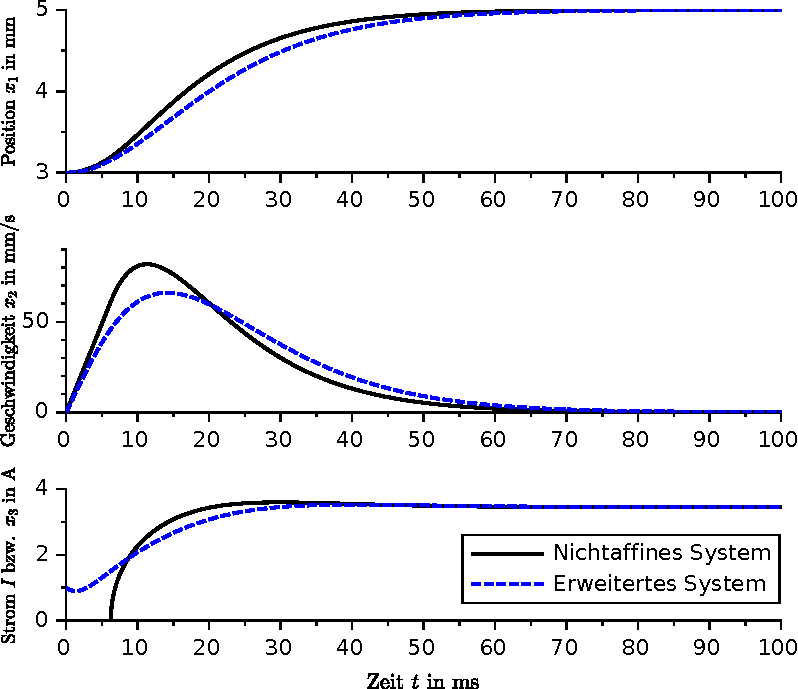
\includegraphics[width=0.85\textwidth]{Kugel_Magnet3}
\par\end{centering}
\caption{Simulation der lagegeregelten Kugel aus den Beispielen~\ref{exa:Kugel-Magnetfeld}
und~\ref{exa:Kugel-Magnetfeld-erweitert}\label{fig:Kugel-Magnet-Simulation-erweitert}}
\end{figure}


\subsection{Byrnes-Isidori-Normalform}

Gegeben sei ein nicht eingangsaffines System~(\ref{eq:Ausgangssystem-nichtaffine-mit-ausgang}).
Dieses System kann immer dargestellt werden in der Form 
\begin{equation}
\dot{x}=F(x,u)=f(x)+\sum_{i=1}^{m}g_{i}(x)\cdot\sigma_{i}(x,u)\label{eq:Vektorfeld-quasi-affin-m}
\end{equation}
mit eingangsunabhängigen Vektorfeldern $f,g_{1},\ldots,g_{m}:\mathcal{M}\to\R^{n}$
und eingangsabhängigen Skalarfeldern $\sigma_{1},\ldots,\sigma_{m}:\mathcal{M}\times\mathcal{U}\to\R$.
Eine solche Darstellung erhält man beispielsweise für $m=n$, indem
man das Vektorfeld~$F$ bezüglich der kanonischen Basis entwickelt:
\[
F(x,u)=F_{1}(x,u)\frac{\partial}{\partial x_{1}}+\cdots+F_{n}(x,u)\frac{\partial}{\partial x_{n}}.
\]

Bei den nachfolgenden Betrachtungen steht die Frage im Vordergrund,
ob die Darstellung~(\ref{eq:Vektorfeld-quasi-affin-m}) für $m=1$
möglich ist. In diesem Fall würde sich das System~(\ref{eq:Ausgangssystem-nichtaffine-mit-ausgang})
in die Form
\begin{equation}
\dot{x}=F(x,u)=f(x)+g(x)\,\sigma(x,u)\label{eq:Vektorfeld-quasi-affin-1}
\end{equation}
zerlegen lassen. Diese Zerlegung ist unter folgenden Bedingungen möglich~\cite{gruenbacher2005}:
\begin{lemma}
\label{lem:umwandlung-nicht-affin-in-quasi-affine}Ein System~(\ref{eq:Ausgangssystem-nichtaffine-mit-ausgang})
kann genau dann für Werte~$u$ aus einer Umgebung von $u_{0}\in\mathcal{U}$
in die Form~(\ref{eq:Vektorfeld-quasi-affin-1}) mit 
\begin{equation}
\left.\frac{\partial\sigma(x,u)}{\partial u}\right|_{u=u_{0}}\neq0\label{eq:quasiaffin-SF-partielle-Abl-u}
\end{equation}
zerlegt werden, wenn das Gleichungssystem
\begin{equation}
F(x,u)-F(x,u_{0})=\left.\frac{\partial F(x,u)}{\partial u}\right|_{u=u_{0}}\cdot\sigma(x,u)\label{eq:bedingung-lin-gls-quasi-affin}
\end{equation}
bezüglich~$\sigma$ lösbar ist. Die Vektorfelder aus Gl.~(\ref{eq:Vektorfeld-quasi-affin-1})
ergeben sich dabei aus
\begin{equation}
f(x)=F(x,u_{0})\quad\text{und}\quad g(x)=\left.\frac{\partial F(x,u)}{\partial u}\right|_{u=u_{0}}.\label{eq:Vektorfelder-f-g-fuer-quasi-affin}
\end{equation}
\end{lemma}
\begin{svmultproof2}
\notwendig\ Gleichungssystem~(\ref{eq:bedingung-lin-gls-quasi-affin})
habe eine Lösung~$\sigma$. Dann ergibt sich die Form~(\ref{eq:Vektorfeld-quasi-affin-1})
unmittelbar aus Gl.~(\ref{eq:Vektorfelder-f-g-fuer-quasi-affin}).

\hinreichend\ System~(\ref{eq:Ausgangssystem-nichtaffine-mit-ausgang})
sei in die Form~(\ref{eq:Vektorfeld-quasi-affin-1}) zerlegbar. Dann
gilt einerseits
\begin{equation}
F(x,u)-F(x,u_{0})=g(x)\cdot\left(\sigma(x,u)-\sigma(x,u_{0})\right),\label{eq:beweis-quasi-affine-t1}
\end{equation}
andererseits 
\begin{equation}
\left.\frac{\partial F(x,u)}{\partial u}\right|_{u=u_{0}}=\left.\frac{\partial}{\partial u}\left(g(x)\,\sigma(x,u)\right)\right|_{u=u_{0}}=g(x)\left.\frac{\partial\sigma(x,u)}{\partial u}\right|_{u=u_{0}}.\label{eq:beweis-quasi-affine-t2}
\end{equation}
Die Vektorfelder~(\ref{eq:beweis-quasi-affine-t1}) und~(\ref{eq:beweis-quasi-affine-t2})
zeigen beide in Richtung des Vektorfeldes~$g$. Wegen $\tfrac{\partial\sigma(x,u)}{\partial u}|_{u=u_{0}}\neq0$
gilt $(F(x,u)-F(x,u_{0}))\in\spann\{g(x)\}$, so dass das (bezüglich~$\sigma$
lineare) Gls.~(\ref{eq:bedingung-lin-gls-quasi-affin}) lösbar ist.
\end{svmultproof2}

In Gl.~(\ref{eq:Vektorfeld-quasi-affin-1}) kann der Eingang nur
in Richtung des von~$u$ unabhängigen Vektorfeldes~$g$ wirken.
In Verbindung mit Gl.~(\ref{eq:beweis-quasi-affine-t2}) bedeutet
das, dass zwar das Vektorfeld $\tfrac{\partial}{\partial u}F(x,u)$
von~$u$ abhängen darf, nicht aber die davon aufgespannte Distribution
$\Delta_{u}:=\im\tfrac{\partial}{\partial u}F(x,u)$.

\begin{example}
\label{exa:Kugel-Magnet-quasi-affine}Man betrachte die im Magnetfeld
schwebende Kugel aus Beispiel~\ref{exa:Kugel-Magnetfeld} mit dem
Eingang $u=I$. Für eine Entwicklungsstelle $u_{0}=I_{0}$ nimmt Gls.~(\ref{eq:bedingung-lin-gls-quasi-affin})
die Form
\[
\left(\begin{array}{c}
0\\
\frac{\rho}{m}\frac{\left(I_{0}^{2}-I^{2}\right)}{(x_{1}+s_{0})^{2}}
\end{array}\right)=\left(\begin{array}{c}
0\\
-2\frac{\rho}{m}\frac{I_{0}^{2}}{(x_{1}+s_{0})^{2}}
\end{array}\right)\cdot\sigma(x,I)
\]
an. Dieses Gleichungssystem ist für $I_{0}\neq0$ lösbar mit $\sigma(I)=-(I_{0}^{2}-I^{2})/(2I_{0})$.
Das zugehörige System~(\ref{eq:Vektorfeld-quasi-affin-1}) lautet
damit 
\[
\dot{x}=\left(\begin{array}{c}
x_{2}\\
g-\frac{\rho}{m}\frac{I_{0}^{2}}{(x_{1}+s_{0})^{2}}
\end{array}\right)+\left(\begin{array}{c}
0\\
-2\frac{\rho}{m}\frac{I_{0}}{(x_{1}+s_{0})^{2}}
\end{array}\right)\cdot\sigma(x,I).
\]
\end{example}

\begin{example}
\label{exa:raumflugkoerper}Wir betrachten einen Raumflugkörper, der
sich außerhalb der Atmosphäre um die Erde bewegt~\cite[S.~193]{nijmeijer90}.
Die Position des Flugkörpers sei in kartesischen Koordinaten durch
$x_{s}=r\cos\theta$ und $y_{s}=r\sin\theta$ mit dem Abstand~$r$
vom Erdmittelpunkt und dem Winkel~$\theta$ gegeben (Abb.~\ref{fig:Raumflugkoerper}).
Daraus ergibt sich die kinetische Energie
\[
T=\frac{m}{2}\left(\dot{x}_{s}^{2}+\dot{y}_{s}^{2}\right)=\frac{m}{2}\left(\dot{r}^{2}+r^{2}\dot{\theta}^{2}\right).
\]
Unter Berücksichtigung des Zentralpotentials erhält man die Lagrange-Funktion
\[
L=\frac{m}{2}\left(\dot{r}^{2}+r^{2}\dot{\theta}^{2}\right)+\frac{mgR^{2}}{r}
\]
mit dem Erdradius~$R$ und der Fallbeschleunigung~$g$ an der Erdoberfläche.
Der Antrieb erzeugt eine konstante Schubkraft~$\digamma$ und ist
über den Winkel~$u$ zu beeinflussen. Daraus ergibt sich folgende
Bewegungsgleichung:
\[
\left(\begin{array}{cc}
m & 0\\
0 & mr^{2}
\end{array}\right)\left(\begin{array}{c}
\ddot{r}\\
\ddot{\theta}
\end{array}\right)+\left(\begin{array}{c}
\frac{mgR^{2}}{r^{2}}-\dot{\theta}^{2}mr\\
2mr\dot{r}\dot{\theta}
\end{array}\right)=\left(\begin{array}{c}
\digamma\cos u\\
\digamma r\sin u
\end{array}\right).
\]
Mit dem Zustand $x=(r,\theta,\dot{r},\dot{\theta})^{T}$ erhält man
das Modell
\begin{equation}
\dot{x}=\left(\begin{array}{c}
x_{3}\\
x_{4}\\
-\frac{gR^{2}}{x_{1}^{2}}+x_{1}x_{4}^{2}+\frac{\digamma}{m}\cos u\\
-2\frac{x_{3}x_{4}}{x_{1}}+\frac{\digamma}{mx_{1}}\sin u
\end{array}\right).\label{eq:Rakete-nichtaffin}
\end{equation}

Es ist zu untersuchen, ob das System~(\ref{eq:Rakete-nichtaffin})
in die Form~(\ref{eq:Vektorfeld-quasi-affin-1}) zerlegt werden kann.
Gls.~(\ref{eq:bedingung-lin-gls-quasi-affin}) hat für $u$ die Form
\[
\left(\begin{array}{c}
0\\
0\\
\frac{\digamma}{m}\left(\cos u-\cos u_{0}\right)\\
\frac{\digamma}{mx_{1}}\left(\sin u-\sin u_{0}\right)
\end{array}\right)=\left(\begin{array}{c}
0\\
0\\
-\frac{\digamma}{m}\sin u_{0}\\
\frac{\digamma}{mx_{1}}\cos u_{0}
\end{array}\right)\cdot\sigma(x,u).
\]
Dieses Gleichungssystem ist in einer Umgebung von~$u_{0}$ nicht
lösbar. Damit gibt es für dieses System keine Darstellung der Form~(\ref{eq:Vektorfeld-quasi-affin-1}).
\end{example}
\begin{figure}
\begin{centering}
\resizebox{0.45\textwidth}{!}{\input{Rakete.pdftex_t}}
\par\end{centering}
\caption{Raumflugkörper außerhalb der Erdatmosphäre\label{fig:Raumflugkoerper}}
\end{figure}

Bei wohldefiniertem relativen Grad (im Sinne von Def.~\ref{def:relativer-Grad-nichtaffine-SISO})
lässt sich ein nicht eingangsaffines System~(\ref{eq:Ausgangssystem-nichtaffine-mit-ausgang})
immer in die Eingangs-Ausgangs-Normalform~(\ref{eq:Eingangs-Ausgangs-NF-nichtaffin})
überführen (Satz~\ref{thm:EA-Form-nicht-affin}). Dabei kann der
Eingang auch im zweiten Teilsystem auftreten. Hängt das zweite Teilsystem
dagegen nicht explizit vom Eingang ab, so geht die Eingangs-Ausgangs-Normalform~(\ref{eq:Eingangs-Ausgangs-NF-nichtaffin})
in die Byrnes-Isidori-Normalform\index{Byrnes-Isidori-Normalform}\index{Normalform!Byrnes-Isidori-}
\begin{equation}
\begin{array}{lcl}
\dot{\xi}_{1} & = & \xi_{2}\\
 & \vdots\\
\dot{\xi}_{r-1} & = & \xi_{r}\\
\dot{\xi}_{r} & = & a(\xi,\eta,u),\quad\text{mit}\quad\frac{\partial}{\partial u}a(\xi,\eta,u)\neq0\\
\dot{\eta}_{r+1} & = & q_{1}(\xi,\eta)\\
 & \vdots\\
\dot{\eta}_{n} & = & q_{n-r}(\xi,\eta)\\
y & = & \xi_{1}
\end{array}\label{eq:BINF-nichtaffin}
\end{equation}
über. Der nächste Satz gibt Auskunft über die Existenzbedingungen
der zugehörigen Transformation:
\begin{theorem}
\label{thm:Bynres-Isidori-nichtaffin}System~(\ref{eq:Ausgangssystem-nichtaffine-mit-ausgang})
habe an der Stelle $(p,u_{0})\in\mathcal{M}\times\mathcal{U}$ den
relativen Grad $r<n$. Das System kann genau dann mit einer Zustandstransformation
in die Byrnes-Isidori-Normalform überführt werden, wenn es in der
Form~(\ref{eq:Vektorfeld-quasi-affin-1}) darstellbar ist.
\end{theorem}
\begin{svmultproof2}
\hinreichend\ System~(\ref{eq:Ausgangssystem-nichtaffine-mit-ausgang})
sei mit $(\xi,\eta)=\Phi(x)$ in die Byrnes-Isidori-Normal\-form~(\ref{eq:BINF-nichtaffin})
transformierbar. Der Eingang~$u$ tritt dann nur in der $r$-ten
Differentialgleichung auf. Die Rücktransformation liefert unmittelbar
die Form~(\ref{eq:Vektorfeld-quasi-affin-1}) mit 
\[
g(x):=\left(\Phi^{\prime}(x)\right)^{-1}\frac{\partial}{\partial\xi_{r}}\quad\text{und}\quad\sigma(x,u):=\alpha(\xi,\eta,u)\quad\text{für}\quad x=\Phi^{-1}(\xi,\eta).
\]

\notwendig\ System~(\ref{eq:Ausgangssystem-nichtaffine-mit-ausgang})
sei in die Form~(\ref{eq:Vektorfeld-quasi-affin-1}) zerlegbar. Bei
wohldefiniertem Grad~$r$ des Systems~(\ref{eq:Ausgangssystem-nichtaffine-mit-ausgang})
im Sinne von Def.~\ref{def:relativer-Grad-nichtaffine-SISO} gilt
\[
\frac{\partial L_{F}^{r-1}h(x,u)}{\partial u}\equiv0\quad\Rightarrow\quad L_{F}^{r-1}h(x,u)=L_{F}^{r-1}h(x)=L_{f}^{r-1}h(x,u)
\]
und
\[
\begin{array}{lcl}
L_{F}^{r}h(x,u) & = & \d L_{F}^{r-1}h(x)\cdot F(x,u)\\
 & = & \d L_{f}^{r-1}h(x)\cdot\left(f(x)+g(x)\cdot\sigma(x,u)\right)\\
 & = & L_{f}^{r}h(x)+L_{g}L_{f}^{r-1}h(x)\cdot\sigma(x,u).
\end{array}
\]
Wegen $\tfrac{\partial}{\partial u}L_{F}^{r}h(x,u)=L_{g}L_{f}^{r-1}h(x)\tfrac{\partial}{\partial u}\sigma(x,u)$
ist damit auch für das sich aus~(\ref{eq:Vektorfeld-quasi-affin-1})
mit dem virtuellen Eingang $\bar{u}:=\sigma(x,u)$ ergebende eingangsaffine
System der relative Grad~$r$ im Sinne von Def.~\ref{def:relativer-Grad-SISO}
wohldefiniert. Dieses System kann in die Byrnes-Isidori-Normalform
überführt werden (Satz~\ref{thm:Byrnes-Isidori-Normalform}). Der
Eingang~$\bar{u}$ tritt nur im ersten Teilsystem auf. Mit dem Einsetzen
von $\sigma(x,u)$ bleibt die Struktur unverändert.
\end{svmultproof2}

\begin{example}
\label{exa:raumflugkoerper-byrnes-isidori}Für den Raumflugkörper
aus Beispiel~\ref{exa:raumflugkoerper} werde der Abstand zum Erdmittelpunkt
als Ausgang gewählt, d.\,h. $y=h(x)=x_{1}$. Der Eingang tritt erstmals
in der zweiten Zeitableitung des Ausgangs auf:
\[
\begin{array}{lclcl}
\dot{y} & = & \dot{x}_{1} & = & x_{3}\\
\ddot{y} & = & \dot{x}_{3} & = & -\frac{gR^{2}}{x_{1}^{2}}+x_{1}x_{4}^{2}+\frac{\digamma}{m}\cos u
\end{array}
\]
Wegen $\partial\ddot{y}/\partial u=-\tfrac{\digamma}{m}\sin u$ ist
der relative Grad $r=2$ für $u\neq i\pi$ mit $i\in\Z$ wohldefiniert.
Da das System nicht in die Form~(\ref{eq:Vektorfeld-quasi-affin-1})
zerlegt werden kann, kann es auch nicht in die Byrnes-Isidori-Normalform
transformiert werden.
\end{example}

Geht man von einem nicht eingangsaffinen Originalsystem~(\ref{eq:Ausgangssystem-nichtaffine-mit-ausgang})
zu dem erweiterten (eingangsaffinen) System~(\ref{eq:nichtaffin-erweitertes-System})
über, so existiert bei wohldefiniertem relativen Grad immer die Byrnes-isidori-Normalform
(Satz~\ref{thm:Byrnes-Isidori-Normalform}). Die zugehörige Koordinatentransformation
des erweiterten Systems~(\ref{eq:nichtaffin-erweitertes-System})
hängt aber nicht nur vom Zustand des Originalsystems~(\ref{eq:Ausgangssystem-nichtaffine-mit-ausgang}),
sondern auch vom Eingang ab.

Wenn der Eingang auf der rechten Seite des zweiten Teilsystems der
Eingangs-Ausgangs-Normalform~(\ref{thm:EA-Form-nicht-affin}) nicht
vollständig zu beseitigen ist kann man zumindest versuchen, den Einfluss
des Eingangs auf dieses Teilsystem zu reduzieren. Durch eine geeignete
Koordinatenwahl lässt sich die Anzahl der Differentialgleichungen
des zweiten Teilsystems, die direkt vom Eingang abhängen, minimieren:

\begin{proposition}
\label{prop:Auftreten-des-Eingangs-EA-NF}System~(\ref{eq:Ausgangssystem-nichtaffine-mit-ausgang})
habe an der Stelle $(p,u_{0})\in\mathcal{M}\times\mathcal{U}$ den
relativen Grad $r<n$. Unter Nutzung der Darstellung~(\ref{eq:Vektorfeld-quasi-affin-m})
habe der involutive Abschluss der von den Eingangsvektorfeldern $g_{1},\ldots,g_{m}$
aufgespannten Distribution in einer Umgebung des Punktes~$p$ die
Dimension 
\[
k:=\dim\inv\left(\spann\{g_{1},\ldots,g_{m}\}\right).
\]
Dann kann die Transformation des Systems in die Eingangs-Ausgangs-Normalform
so gewählt werden, dass der Eingang~$u$ nur in $k-1$ Differentialgleichungen
des zweiten Teilsystems auftritt.
\end{proposition}
\begin{proofsketch}Die Distribution $\Delta:=\inv(\spann\{g_{1},\ldots,g_{m}\}$
ist laut Annahme regulär und involutiv. Dann exisitieren eine Umgebung
$\mathcal{U}\subseteq\mathcal{M}$ von~$p$ und $n-k$ Skalarfelder
$\lambda_{1},\ldots,\lambda_{n-k}:\mathcal{U}\to\R$, so dass die
zugehörigen Gradienten $\d\lambda_{1},\ldots,\d\lambda_{n-k}$ den
Annihilator~$\Delta^{\perp}$ aufspannen. Die Skalarfelder $\lambda_{1},\ldots,\lambda_{n-k}$
kann man durch weitere Skalarfelder $\lambda_{n-k+1},\ldots,\lambda_{n}$
zu einer Koordinatentransformation $z=\lambda(x)$ mit $z_{i}=\lambda_{i}(x)$
für $i=1,\ldots,n$ ergänzen (Korollar~\ref{cor:ergaenzung-einer-kodistribution-integrierbar}).
Mit der Zugehörigkeit der ersten $n-k$ Funktionen zum Annihilator~$\Delta^{\perp}$
gilt $\langle\d\lambda_{i},g\rangle=L_{g}\lambda_{i}=0$ für $i=1,\ldots,n-k$
und alle $g\in\Delta$. Die verbleibenden $k$ Funktionen gehören
nicht zum Annihilator, so dass $\langle\d\lambda_{i},g\rangle=L_{g}\lambda_{i}\neq0$
für $i=n-k+1,\ldots,n$. Jeder Term $L_{g}\lambda_{i}\neq0$ führt
dazu, dass der Eingang~$u$ in der $i$-ten Gleichung der transformieten
Koordinaten auftritt.

Bei einem relativen Grad~$r$ existiert die Eingangs-Ausgangs-Normalform~(\ref{eq:Eingangs-Ausgangs-NF-nichtaffin}).
Der Eingang tritt im ersten Teilsystem in genau einer (nämlich der
letzten) Zeile auf. Durch passende Koordinatenwahl tritt der Eingang
im zweiten Teilsystem nur noch in $k-1$ Gleichungen in Erscheinung.\end{proofsketch}
\begin{example}
\label{exa:raumflugkoerper-EA-NF-reduziert}Betrachtet werde der Raumflugkörper
aus Beispiel~\ref{exa:raumflugkoerper} mit dem Ausgang aus Beispiel~\ref{exa:raumflugkoerper-byrnes-isidori}.
Das System kann in die Form~(\ref{eq:Vektorfeld-quasi-affin-m})
mit
\[
\dot{x}=F(x,u)=\underbrace{\left(\begin{array}{c}
x_{3}\\
x_{4}\\
-\frac{gR^{2}}{x_{1}^{2}}+x_{1}x_{4}^{2}\\
-2\frac{x_{3}x_{4}}{x_{1}}
\end{array}\right)}_{{\displaystyle f(x)}}+\underbrace{\left(\begin{array}{c}
0\\
0\\
\frac{\digamma}{m}\\
0
\end{array}\right)}_{{\displaystyle g}_{1}(x)}\cos u+\underbrace{\left(\begin{array}{c}
0\\
0\\
0\\
\frac{\digamma}{mx_{1}}
\end{array}\right)}_{{\displaystyle g}_{2}(x)}\sin u
\]
zerlegt werden. Die Distribution $\Delta=\spann\{g_{1},g_{2}\}$ ist
für $x_{1}\neq0$ definiert und mit $[g_{1},g_{2}]=0$ involutiv (d.\,h.
$\Delta=\inv(\Delta)$). Damit gilt $k=2$. Die Koordinaten lassen
sich so wählen, dass der Eingang nur in $k-1=1$ mal im zweiten Teilsystem
auftritt. Mit einer Umbenennung der Zustandskomponenten überführt
man~(\ref{eq:Rakete-nichtaffin}) in die Eingangs-Ausgangs-Normalform
\[
\begin{array}{lcl}
\dot{\xi}_{1} & = & \xi_{2}\\
\dot{\xi}_{2} & = & -\frac{gR^{2}}{\xi_{1}^{2}}+\xi_{1}\eta_{2}^{2}+\frac{\digamma}{m}\cos u\\
\dot{\eta}_{1} & = & \eta_{2}\\
\dot{\eta}_{2} & = & -2\frac{\xi_{2}\eta_{2}}{\xi_{1}}+\frac{\digamma}{m\xi_{1}}\sin u\\
y & = & \xi_{1}.
\end{array}
\]
Wie erwartet tritt der Eingang nur in einer der beiden Differentialgleichung
des zweiten Teilsystems auf.
\end{example}

\subsection{Eingangs-Zustands-Linearisierung und Regelungsnormalform}

In Analogie zu Abschnitt~\ref{sec:Exakte-Eingangs-Zustands-Linearisierung}
nennen wir ein nicht eingangsaffines System
\begin{equation}
\dot{x}=F(x,u)\label{eq:Ausgangssystem-nichtaffine-ohne-ausgang}
\end{equation}
mit dem eingangsabhängigen Vektorfelder $F:\mathcal{M}\times\mathcal{U}\to\R^{n}$
\emph{eingangs-zustands-linearisierbar}\index{eingangs-zustands-linearisierbar},
wenn ein Skalarfeld $h:\mathcal{M}\to\R$ exisitert, mit welchem das
resultierende System~(\ref{eq:Ausgangssystem-nichtaffine-mit-ausgang})
den relativen Grad~$n$ besitzt. In diesem Fall ist die zugehörigen
Eingangs-Ausgangs-Normalform~(\ref{eq:Eingangs-Ausgangs-NF-nichtaffin})
gleichzeitig die Regelungsnormalform\index{Regelungsnormalform}\index{Normalform!Regelungs-}
\begin{equation}
\begin{array}{lcl}
\dot{\xi}_{1} & = & \xi_{2}\\
 & \vdots\\
\dot{\xi}_{n-1} & = & \xi_{n}\\
\dot{\xi}_{n} & = & a(\xi,u),\quad\text{mit}\quad\frac{\partial}{\partial u}a(\xi,u)\neq0\\
y & = & \xi_{1}
\end{array}\label{eq:Regelungs-NF-nichtaffin}
\end{equation}
 des nicht eingangsaffinen Systems~(\ref{eq:Ausgangssystem-nichtaffine-mit-ausgang}).

\begin{theorem}
\label{thm:EZ-Linearisierung-nichtaffin}Wir betrachten System~(\ref{eq:Ausgangssystem-nichtaffine-ohne-ausgang})
in einer Umgebung von $(p,u^{0})\in\mathcal{M}\times\mathcal{U}$.
Dann sind folgende Aussagen äquivalent:
\begin{enumerate}
\item \label{enu:EZL-nichtaffin1}System~(\ref{eq:Ausgangssystem-nichtaffine-ohne-ausgang})
ist eingangs-zustands-linearisierbar.
\item \label{enu:EZL-nichtaffin2}System~(\ref{eq:Ausgangssystem-nichtaffine-ohne-ausgang})
kann in die Form~(\ref{eq:Vektorfeld-quasi-affin-1}) mit~(\ref{eq:quasiaffin-SF-partielle-Abl-u})
zerlegt werden und das aus den Vektorfeldern~$f$ und~$g$ resultierende
eingangsaffine Ersatz\-system
\begin{equation}
\dot{x}=f(x)+g(x)\bar{u}\label{eq:affines-ersatzsystem-nach-zerlegung}
\end{equation}
ist eingangs-zustands-linearisierbar.
\item \label{enu:EZL-nichtaffin3}Das erweiterte System~(\ref{eq:nichtaffin-erweitertes-System2})
ist eingangs-zustands-linearisierbar.
\end{enumerate}
\end{theorem}

\begin{svmultproof2}
(1)~$\Rightarrow$~(2): System~(\ref{eq:Ausgangssystem-nichtaffine-ohne-ausgang})
sei eingangs-zustands-linearisierbar, d.\,h. es gibt einen Diffeomorphismus
$\xi=\Phi(x)$, der System~(\ref{eq:Ausgangssystem-nichtaffine-ohne-ausgang})
in die Regelungsnormalform~(\ref{eq:Regelungs-NF-nichtaffin}) überführt.
Das transformierte System~(\ref{eq:Regelungs-NF-nichtaffin}) liegt
bereits in der Form~(\ref{eq:Vektorfeld-quasi-affin-1}) vor. Die
Zerlegung~(\ref{eq:Vektorfeld-quasi-affin-1}) ergibt sich in den
Originalkoordinaten aus 
\[
g(x):=\left(\Phi^{\prime}(x)\right)^{-1}\frac{\partial}{\partial\xi_{n}}\quad\text{und}\quad\sigma(x,u):=\alpha(\xi,u)\quad\text{für}\quad x=\Phi^{-1}(\xi),
\]
vgl. Beweis von Satz~\ref{thm:EA-Form-nicht-affin}. Mit der angegebenen
Festlegung des Eingangsvektorfeldes ist zugehörige Ersatzsystem~(\ref{eq:affines-ersatzsystem-nach-zerlegung})
eingangs-zustands-linearisierbar, da in den durch die Transformation~$\Phi$
induzierten Koordinaten die spezielle Regelungsnormalform~(\ref{eq:regelungsnormalform-eingeschraenkt})
vorliegt.

(2)~$\Rightarrow$~(1): Das System liege in der Form~(\ref{eq:Vektorfeld-quasi-affin-1})
vor und das zugehörige Ersatzsystem~(\ref{eq:affines-ersatzsystem-nach-zerlegung})
sei eingangs-zustands-linarisierbar. Die Transformation des Ersatzsystems
in die (eingangsaffine) Regelungsnormalform~(\ref{eq:Regelungsnormalform})
und Einsetzen von $\bar{u}=\sigma(x,u)$ liefert die Regelungsnormalform~(\ref{eq:Regelungs-NF-nichtaffin}),
wobei sich $\frac{\partial}{\partial u}a(\xi,u)\neq0$ aus~(\ref{eq:quasiaffin-SF-partielle-Abl-u})
ergibt. Das nicht eingangsaffine System~(\ref{eq:Ausgangssystem-nichtaffine-ohne-ausgang})
ist also eingangs-zustands-linearisierbar.

(1)~$\Rightarrow$~(3): System~(\ref{eq:Ausgangssystem-nichtaffine-ohne-ausgang})
sei mit $\xi=\Phi(x)$ in die Regelungsnormalform~(\ref{eq:Regelungs-NF-nichtaffin})
überführbar. Bedingt durch $\frac{\partial}{\partial u}a(\xi,u)\neq0$
kann insbesondere auch die Nichtlinearität~$\alpha$ (zumindest lokal)
mit $\alpha(\xi,u)\stackrel{!}{=}v$ kompensiert werden (Satz über
die Umkehrfunktion). Die Ableitung 
\[
\dot{v}=\underbrace{\frac{\partial}{\partial\xi}a(\xi,u)\dot{\xi}}_{{\displaystyle \tilde{\alpha}(\xi,v)}}+\underbrace{\frac{\partial}{\partial u}a(\xi,u)}_{{\displaystyle \tilde{\beta}(\xi,v)}}\dot{u}
\]
führt mit $\dot{u}=\tilde{u}$ auf die Regelungsnormalform 
\[
\begin{array}{lcl}
\dot{\xi}_{1} & = & \xi_{2}\\
 & \vdots\\
\dot{\xi}_{n-1} & = & \xi_{n}\\
\dot{\xi}_{n} & = & v\\
\dot{v} & = & \tilde{\alpha}(\xi,v)+\tilde{\beta}(\xi,v)\tilde{u}.
\end{array}
\]
des erweiterten Systems~(\ref{eq:nichtaffin-erweitertes-System2}).
Die Transformation des erweiterten Systems~(\ref{eq:nichtaffin-erweitertes-System2})
wird durch
\[
\tilde{\Phi}:\quad\tilde{x}=\left(\begin{array}{c}
x\\
u
\end{array}\right)\mapsto\left(\begin{array}{c}
\xi\\
v
\end{array}\right)=\left(\begin{array}{c}
\Phi(x)\\
\alpha(\Phi(x),u)
\end{array}\right)
\]
beschrieben. Die zugehörige Jacobimatrix
\[
\tilde{\Phi}^{\prime}(\tilde{x})=\tilde{\Phi}^{\prime}(x,u)=\left(\begin{array}{cc}
\Phi^{\prime}(x) & 0\\
* & \frac{\partial}{\partial u}a(\xi,u)
\end{array}\right)
\]
ist regulär.

(3)~$\Rightarrow$~(1): Das erweiterte Systems~(\ref{eq:nichtaffin-erweitertes-System2})
sei eingangs-zustands-linearisierbar. Damit gibt es einen Ausgang~$\tilde{h}$,
für den das erweiterte System~(\ref{eq:nichtaffin-erweitertes-System2})
den relativen Grad $n+1$ besitzt. Daraus erhält man einen Ausgang~$h$
des Originalsystems~(\ref{eq:Ausgangssystem-nichtaffine-ohne-ausgang})
mit dem relativen Grad~$n$ (vgl. Prop.~\ref{prop:relativer-Grad-erweitertes-System}).
\end{svmultproof2}

Die Bedingung~\ref{enu:EZL-nichtaffin3} von Satz~\ref{thm:EZ-Linearisierung-nichtaffin}
lässt sich über Satz~\ref{thm:Exakte-Eingangs-Zustands_Linearisierung}
bzw. Satz~\ref{thm:Exakte-Eingangs-Zustands-Linearisierung-Formen}
überprüfen. Bei Bedingung~\ref{enu:EZL-nichtaffin2} ist zusätzlich
Lemma~\ref{lem:umwandlung-nicht-affin-in-quasi-affine} zu beachten.
Insbesondere wird man bei den Bedingungen~\ref{enu:EZL-nichtaffin2}
und~\ref{enu:EZL-nichtaffin3} auf eingangsaffine Vergleichssysteme~(\ref{eq:nichtaffin-erweitertes-System2})
und~(\ref{eq:Vektorfeld-quasi-affin-1}) geführt und kann damit die
in Abschnitt~\ref{sec:Exakte-Eingangs-Zustands-Linearisierung} beschriebenen
Ansätze zur Berechnung eines Ausgangs mit vollem relativen Grad nutzen.

\begin{example}
Man betrachte den Raumflugkörper aus Beispiel~\ref{exa:raumflugkoerper}.
Es wurde gezeigt, dass das System~(\ref{eq:Rakete-nichtaffin}) nicht
in die Form~(\ref{eq:Vektorfeld-quasi-affin-1}) zerlegt werden kann.
Daher ist das System auch nicht eingangs-zustands-linearisierbar.
\end{example}

\begin{example}
\label{exa:Dreirad-Modell-EZ-SISO}Wir modifizieren den zweirädrigen
mobilen Roboter aus Abschnitt~\ref{subsec:Mobiler-Roboter-Modellierung}
zu dem in Abb.~\ref{fig:dreirad} gezeigten dreirädrigen Roboter.
Der Antrieb erfolgt jetzt über die im Gleichlauf betriebenen Räder
der Hinterachse und resultiert in einer in Fahrtrichtung orientierten
Geschwindigkeit~$v$. Daraus ergibt sich die translatorische Bewegung
\begin{equation}
\begin{array}{lcl}
\dot{x}_{1} & = & v\,\sin\varphi,\\
\dot{x}_{2} & = & v\,\cos\varphi.
\end{array}\label{eq:dreirad-modell-trans}
\end{equation}
Zusätzlich kann über das erste Rad der Lenkwinkel~$\delta$ eingestellt
werden. Für das sich aus Hinterachsmittelpunkt, Vorderachse und dem
Kreismittelpunkt~$P$ ergebende rechtwinklige Dreieck gilt 
\begin{equation}
\tan\delta=\frac{D}{R},\label{dreirad-lenkwinkel}
\end{equation}
wobei~$D$ den Abstand zwischen Vorder- und Hinterachse bezeichnet.
Für die Bewegung auf der (fiktiven) Kreisbahn besteht zwischen der
translatorischen Geschwindigkeit~$v$ und der Winkelgeschwindigkeit~$\dot{\varphi}$
die Beziehung $v=R\dot{\varphi}$, womit der Kreisradius~$R$ aus
Gl.~(\ref{dreirad-lenkwinkel}) eliminiert werden kann. Mit $x_{3}=\varphi$
erhält man insgesamt das kinematische Modell
\begin{equation}
\begin{array}{lcl}
\dot{x}_{1} & = & v\,\sin x_{3},\\
\dot{x}_{2} & = & v\,\cos x_{3},\\
\dot{x}_{3} & = & \frac{v}{D}\,\tan\delta.
\end{array}\label{eq:dreirad-kinematisches-modell}
\end{equation}

\begin{figure}
\begin{centering}
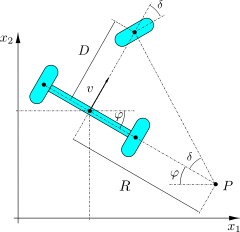
\includegraphics[width=0.48\textwidth]{Roboter_drei_Raeder}
\par\end{centering}
\caption{Mobiler Roboter in der $(x_{1},x_{2})$-Ebene\label{fig:dreirad}}
\end{figure}

Beeinflusst man den dreirädrigen Roboter nur über den Lenkwinkel~$\delta$
bei konstanter Geschwindigkeit $v>0$, so liegt mit Gl.~(\ref{eq:dreirad-kinematisches-modell})
ein nicht eingangsaffines Eingrößensystem vor, welches sich unmittelbar
in die Form~(\ref{eq:Vektorfeld-quasi-affin-1}) zerlegten lässt:
\[
\left(\begin{array}{c}
\dot{x}_{1}\\
\dot{x}_{2}\\
\dot{x}_{3}
\end{array}\right)=\underbrace{\left(\begin{array}{c}
v\,\sin x_{3}\\
v\,\cos x_{3}\\
0
\end{array}\right)}_{{\displaystyle f(x)}}+\underbrace{\left(\begin{array}{c}
0\\
0\\
\frac{v}{D}
\end{array}\right)}_{{\displaystyle g(x)}}\cdot\tan\delta.
\]
Die Vektorfelder~$f$ und~$g$ stimmen bis auf jeweils einen konstanten
Faktor mit den entsprechenden Vektorfeldern des mobilen Roboters überein.
In Beispiel~\ref{exa:Roboter-eingangs-zustands-linearisierung} wurde
gezeigt, dass das zugehörige System nicht eingangs-zustands-linearisierbar
ist. Gemäß Satz~\ref{thm:EZ-Linearisierung-nichtaffin} ist damit
auch das nichtaffine Modell~(\ref{eq:dreirad-kinematisches-modell})
in der hier betrachteten Eingangskonstellation nicht eingangs-zustands-linearisierbar.
\end{example}

\section{Flache Systeme\label{sec:Flache-Systeme}}

\subsection{Definition und Einführungsbeispiele}

Mit der Formulierung des Flachheitsbegriffs im Kontext der Regelungstheorie
gelang es Mitte der neunziger Jahre der Forschergruppe um Michel Fliess
einen mathematischen Rahmen zu schaffen, der den systematischen Entwurf
von Steuerung und Regelung für eine große Klasse nichtlinearer Systeme
ermöglicht~\cite{FLMR95ijc}. Eine zentrale Größe bei dieser Herangehensweise
ist der sog. flache Ausgang, der eine integralfreie Parametrierung
aller Systemgrößen ermöglicht.

Unsere Betrachtungen beschränken sich auf Zustandsraummodelle der
Form 
\begin{equation}
\dot{x}=F(x,u)\label{eq:Ausgangssystem-Flachheit-MIMO}
\end{equation}
mit einem hinreichend glatten eingangsabhängigen Vektorfeld $F:\mathcal{M}\times\mathcal{U}\to\R^{n}$,
das auf einer offenen Teilmenge $\mathcal{M}\subseteq\R^{n}$ und
einer weiteren Teilmenge $\mathcal{U}\subseteq\R^{m}$ definiert ist.
Für diese Systemklasse lässt sich der die Flachheit wie folgt definieren~\cite{rudolph2003habil}:
\begin{definition}
\label{def:flach}Das System~(\ref{eq:Ausgangssystem-Flachheit-MIMO})
heißt \emph{(differentiell) flach}\index{flach}, wenn es ein $m$-Tupel
$\zeta:=(\zeta_{1},\ldots,\zeta_{m})^{T}$ sowie glatte Funktionen~$\Psi,\Theta$
gibt, so dass
\begin{enumerate}
\item \label{enu:flach1}$x=\Psi(\zeta,\dot{\zeta},\ldots,\zeta^{(n_{x})})$
mit $n_{x}<\infty$ und
\item \label{enu:flach2}$u=\Theta(\zeta,\dot{\zeta},\ldots,\zeta^{(n_{u})})$
mit $n_{u}<\infty$.
\end{enumerate}
Dann heißt~$\zeta$ \emph{flacher Ausgang}.
\end{definition}

Die Existenz eines flachen Ausgangs nach Def.~\ref{def:flach} bedeutet,
dass die in Gl.~(\ref{eq:Ausgangssystem-Flachheit-MIMO}) auftretenden
Systemgrößen, nämlich der Zustand~$x$ und der Eingang~$u$, eindeutig
aus dem Verlauf des flachen Ausgangs~$\zeta$ und einer endlichen
Anzahl von Zeitableitungen bestimmt werden können. Man spricht dabei
auch von einer integralfreien Parametrierung aller Systemgrößen, da
zur Bestimmung der Systemgrößen keine Integration im Sinne des Lösens
von Differentialgleichungen erforderlich ist. Bei der Definition der
Flachheit wird zusätzlich oft die differentielle Unabhängigkeit der
Komponenten~$\zeta_{i}$ des Tupels~$\zeta$ gefordert. Diese Forderung
ist hier nicht nötig~\cite{fliess1999}. Allerdings muss die Dimension
des flachen Ausgangs~$\zeta$ mit der Dimension des Eingangsvektors~$u$
übereinstimmen.

In der Regel werden die in Def.~\ref{def:flach} angegebenen Abbildungen~$\Psi$
und~$\Theta$ nicht global für alle Werte von $(\zeta,\dot{\zeta},\ddot{\zeta},\ldots)$
definiert sein. Sind diese Abbdilungen auf einer offenen und nicht
leeren Teilmenge definiert, dann nennt man das System~(\ref{eq:Ausgangssystem-Flachheit-MIMO})
\emph{lokal flach} bzw. spricht von einem \emph{lokal flachen Ausgang}~\cite{levine2007equivalence,levine2011}.
Da bei praxisrelevanten Systemen die entsprechenden Abbildungen nahezu
immer Ausnahmepunkte (Singularitäten) besitzen, werden wir die Begriffe
flach und lokal flach synonym verwenden.

Der flache Ausgang muss nicht notwendigerweise mit dem technischen
Ausgang dieses Systems übereinstimmen. Vielmehr ist der flache Ausgang
eine Hilfsgröße, die für den Entwurf einer Steuerung bzw. einer Regelung
hilfreich ist. Bei Eingrößensystemen sind die Existenzbedingungen
für einen flachen Ausgang bekannt (siehe Abschnitt~\ref{subsec:Flacher-nichtflacher-Ausgang}).
Im Mehrgrößenfall ist der Test eines Systems auf Flachheit bzw. die
Berechnung eines flachen Ausgangs trotz zahlreicher theoretischer
Fortschritte bisher nicht abschließend gelöst~\cite{levine2011,schoeberl2012at,verhoeven2013,franke2014diss,fritzsche2016at}. 

In vielen Anwendungsfällen ergibt sich der flache Ausgang aus der
Regelungsaufgabe bzw. besitzt eine physikalische Bedeutung. Diese
Situation wird zunächst an einem Eingrößensystem illustriert~\cite{sira-ramirez2002converter,gensior2006}:

\begin{example}
\label{exa:Hochsetzsteller-flach}Das gemittelte Modell des in Abschnitt~\ref{subsec:Hochsetzsteller-Modellierung}
beschriebenen Hochsetzstellers
\begin{equation}
\begin{array}{lcl}
\dot{x}_{1} & = & -(1-u)\frac{1}{L}x_{2}+\frac{E}{L}\\
\dot{x}_{2} & = & (1-u)\frac{1}{C}x_{1}-\frac{1}{RC}x_{2}
\end{array}\label{eq:hochsetzsteller-system-flachheit}
\end{equation}
besitzt den flachen Ausgang
\begin{equation}
\zeta=\frac{L}{2}x_{1}^{2}+\frac{C}{2}x_{2}^{2}.\label{eq:hochsetz-y}
\end{equation}
Physikalisch ist diese Größe als die in der Spule und im Kondensator
gespeicherte elektrische Energie zu verstehen. Die zeitliche Ableitung
des flachen Ausgangs~(\ref{eq:hochsetz-y}) vereinfacht sich unter
Einsetzen der Systemdynamik~(\ref{eq:hochsetzsteller-system-flachheit})
zu
\begin{equation}
\begin{array}{rcl}
\dot{\zeta} & = & Lx_{1}\dot{x}_{1}+Cx_{2}\dot{x}_{2}\\
 & = & Ex_{1}-\frac{1}{R}x_{2}^{2}.
\end{array}\label{eq:hochsetz-dy}
\end{equation}
Durch Eliminination der Variablen~$x_{2}$ aus den Gleichungen~(\ref{eq:hochsetz-y})
und~(\ref{eq:hochsetz-dy}) erhält man die erste Zustandsvariable
\begin{equation}
x_{1}=\psi_{1}(\zeta,\dot{\zeta})=\sqrt{\frac{R^{2}C^{2}E^{2}}{4L^{2}}+\frac{2}{L}\zeta+\frac{RC}{L}\dot{\zeta}}-\frac{RCE}{2L},\label{eq:hochsetz-flach-x1}
\end{equation}
unter Ausnutzung dieses Zwischenergebnisses in Verbindung mit~(\ref{eq:hochsetz-dy})
die zweite Zustandsvariable:
\begin{equation}
x_{2}=\psi_{2}(\zeta,\dot{\zeta})=\sqrt{R\left(E\psi_{1}(\zeta,\dot{\zeta})-\dot{\zeta}\right)}.\label{eq:hochsetz-flach-x2}
\end{equation}
Der Eingang tritt in der zweiten Zeitableitung des flachen Ausgangs
auf:
\begin{equation}
\begin{array}{rcl}
\ddot{\zeta} & = & E\dot{x}_{1}-\frac{2}{R}x_{2}\dot{x}_{2}\\
 & = & \frac{E}{L}\left(E+(u-1)x_{2}\right)+\frac{2}{RC}x_{2}\left((u-1)x_{1}+\frac{1}{R}x_{2}\right).
\end{array}\label{eq:hochsetz-ddy}
\end{equation}
Durch Umstellen nach~$u$ und Einsetzen von~(\ref{eq:hochsetz-flach-x1})
und~(\ref{eq:hochsetz-flach-x2}) erhält man die Parametrierung
\[
\begin{array}{cll}
u & = & 1-\frac{R^{2}C\left(E^{2}-L\ddot{\zeta}\right)+2Lx_{2}^{2}}{Rx_{2}\left(RCE+2Lx_{1}\right)}\\
 & = & 1-\frac{R^{2}C\left(E^{2}-L\ddot{\zeta}\right)+2L\psi_{2}^{2}(\zeta,\dot{\zeta})}{R\psi_{2}(\zeta,\dot{\zeta})\left(RCE+2L\psi_{1}(\zeta,\dot{\zeta})\right)}.\\
 & =: & \Theta(\zeta,\dot{\zeta},\ddot{\zeta})
\end{array}
\]
des Eingangs.
\end{example}

Im nächsten Beispiel wird ein Mehrgrößensystem betrachtet~\cite{rothfuss97flach,ryu2011}:
\begin{example}
\label{exa:Mobiler-Roboter-Flachheit}Man betrachte das kinematische
Modell
\begin{equation}
\dot{x}=\left(\begin{array}{c}
\sin x_{3}\\
\cos x_{3}\\
0
\end{array}\right)u_{1}+\left(\begin{array}{c}
0\\
0\\
1
\end{array}\right)u_{2}\label{eq:mobiler-roboter-MIMO-modell-flachheit}
\end{equation}
des mobilen Roboters aus Abschnitt~\ref{subsec:Mobiler-Roboter-Modellierung}
mit den Eingängen~$u_{1}$ und~$u_{2}$. Es wird nachfolgend gezeigt,
dass die Position des Roboters in der Ebene einen flachen Ausgang
darstellt, also $\zeta=(\zeta_{1},\zeta_{2})^{T}=(x_{1},x_{2})^{T}$.
Aus dem Quotienten der ersten beiden Differentialgleichungen~(\ref{eq:mobiler-roboter-MIMO-modell-flachheit})
ergibt sich 
\[
\frac{\dot{x}_{1}}{\dot{x}_{2}}=\frac{\sin x_{3}}{\cos x_{3}}=\tan x_{3}\quad\text{bzw.}\quad x_{3}=\arctan\left(\frac{\dot{x}_{1}}{\dot{x}_{2}}\right).
\]
Damit erhält man die Abbildung~$\Psi$ aus Bedingung~\ref{enu:flach1}
von Def.~\ref{def:flach}:
\[
x=\Psi(\zeta,\dot{\zeta})=\left(\begin{array}{c}
\zeta_{1}\\
\zeta_{2}\\
\arctan\frac{\dot{\zeta}_{1}}{\dot{\zeta}_{2}}
\end{array}\right).
\]
Aus der Summe der Quadrate der ersten zwei Systemgleichungen 
\[
\dot{x}_{1}^{2}+\dot{x}_{2}^{2}=u_{1}^{2}\sin^{2}x_{3}+u_{1}^{2}\cos^{2}x_{3}=u_{1}^{2}
\]
erhält man die Parametrierung
\[
u_{1}=\theta_{1}(\zeta,\dot{\zeta})=\pm\sqrt{\dot{\zeta}_{1}^{2}+\dot{\zeta}_{2}^{2}}
\]
des ersten Eingangs, aus der dritten Systemgleichung ergibt sich die
Parametrierung des zweiten Eingangs: 
\[
\begin{array}{lll}
u_{2} & = & \dot{x}_{3}\\
 & = & \frac{\d}{\d t}\arctan\frac{\dot{x}_{1}}{\dot{x}_{2}}\\
 & = & \left.\frac{\dot{z}}{1+z^{2}}\right|_{z=\dot{\zeta}_{1}/\dot{\zeta}_{2}}\\
 & = & \frac{\ddot{\zeta}_{1}\dot{\zeta}_{2}-\dot{\zeta}_{1}\ddot{\zeta}_{2}}{\dot{\zeta}_{1}^{2}+\dot{\zeta}_{2}^{2}}\\
 & =: & \theta_{2}(\zeta,\dot{\zeta},\ddot{\zeta}).
\end{array}
\]
Damit liegt eine vollständige Parametrierung aller Systemgrößen vor.
\end{example}

\subsection{Zusammenhang zwischen flachem Ausgang und Systemausgang für Eingrößensysteme\label{subsec:Flacher-nichtflacher-Ausgang}}

Man betrachte System~(\ref{eq:Ausgangssystem-Flachheit-MIMO}) mit
$m=1$, d.\,h. wir beschränken uns in diesem Abschnitt auf Systeme
mit einem (skalarwertigen) Eingang. Die Flachheit eines derartigen
Eingrößensystems lässt sich folgendermaßen charakterisieren~\cite{nieuwstadt1994}:
\begin{theorem}
\label{thm:flach-EZ-lin-SISO}Ein Eingrößensystem~(\ref{eq:Ausgangssystem-Flachheit-MIMO})
ist genau dann (lokal) flach, wenn es (lokal) exakt eingangs-zustands-linearisierbar
ist. Ein flacher Ausgang hat den relativen Grad~$n$.
\end{theorem}
\begin{svmultproof2}
\notwendig\ System~(\ref{eq:Ausgangssystem-Flachheit-MIMO}) sei
exakt eingangs-zustands-linearisierbar, d.\,h. es existiert eine
Ausgangsabbildung $h:\mathcal{M}\to\R$, für die das System den relativen
Grad~$n$ besitzt. Wir setzen $\zeta=h(x)$. Durch den wohldefinierten
relativen Grad $r=n$ kann das System~(\ref{eq:Ausgangssystem-Flachheit-MIMO})
mit einem Diffeomorphismus $\xi=\Phi(x)$ in die Regelungsnormalform~(\ref{eq:Regelungs-NF-nichtaffin})
transformiert werden. Zwischen dem Ausgang~$\zeta$ und den Zuständen~$\xi$
bestehen folgende Beziehungen:
\[
\zeta=\xi_{1},\;\dot{\zeta}=\xi_{2},\;\ddot{\zeta}=\xi_{3},\;\ldots,\zeta^{(n-1)}=\xi_{n}.
\]
Da~$\Phi$ ein Diffeomorphismus ist, existiert die Umkehrabbildung
\[
\begin{array}{lll}
x & = & \Phi^{-1}(\xi)\\
 & = & \Phi^{-1}(\xi_{1},\xi_{2},\ldots,\xi_{n})\\
 & = & \Phi^{-1}(\zeta,\dot{\zeta},\ldots,\zeta^{(n-1)})\\
 & =: & \Psi(\zeta,\dot{\zeta},\ldots,\zeta^{(n-1)}),
\end{array}
\]
so dass Bedingung~\ref{enu:flach1} aus Def.~\ref{def:flach} erfüllt
ist. Wegen $\tfrac{\partial}{\partial u}\alpha(\xi,u)\neq0$ kann~$\alpha$
bezüglich des zweiten Arguments invertiert werden, d.\,h. es gibt
eine Umkehrabbildung~$\alpha^{-1}$ mit 
\[
u=\alpha^{-1}(\xi,\dot{\xi}_{n})=:\Theta(\zeta,\dot{\zeta},\ldots,\zeta^{(n-1)},\zeta^{(n)}).
\]
Damit ist auch Bedingung~\ref{enu:flach2} aus Def.~\ref{def:flach}
erfüllt. Der Ausgang~$\zeta$ ist folglich ein flacher Ausgang von~(\ref{eq:Ausgangssystem-Flachheit-MIMO}).

\hinreichend\ System~(\ref{eq:Ausgangssystem-Flachheit-MIMO}) sei
flach, d.\,h. es gibt einen flachen Ausgang~$\zeta$ und Abbildungen~$\Psi,\Theta$
nach Def.~\ref{def:flach}. Sei $n_{u}$ die höchste Ableitungsordnung
des flachen Ausgangs, durch welche der Eingang~$u$ direkt beeinflusst
wird. Dann kann man die Bedingung~\ref{enu:flach1} von Def.~\ref{def:flach}
lokal nach~$\zeta^{(n_{u})}$ auflösen und erhält eine Beziehung
der Form
\begin{equation}
\zeta^{(n_{u})}=\varUpsilon\left(\zeta,\dot{\zeta},\ldots,\zeta^{(n_{u}-1)},u\right).\label{eq:flache-Paramrierung-SISO-aufgeloest}
\end{equation}
Mit Gl.~(\ref{eq:flache-Paramrierung-SISO-aufgeloest}) bekommt man
eine Eingangs-Ausgangs-Beschreibung des Systems~(\ref{eq:Ausgangssystem-Flachheit-MIMO}).
Mit $z_{1}=\zeta,z_{2}=\dot{\zeta},\ldots,z_{n_{u}}=\zeta^{(n_{u}-1)}$
könnte man aus~(\ref{eq:flache-Paramrierung-SISO-aufgeloest}) eine
(eventuell nicht alle Zustände des Originalsystems~(\ref{eq:Ausgangssystem-Flachheit-MIMO})
erfassende) Zustandsbeschreibung erhalten. Aus der Darstellung~(\ref{eq:flache-Paramrierung-SISO-aufgeloest})
ergibt sich unmittelbar ein relativer Grad~$n_{u}$ (vgl. Abschnitt~\ref{subsec:Relativer-Grad-nichtaffine}).

Angenommen, es gelte $n_{u}<n$. Dann würde das System~(\ref{eq:Ausgangssystem-Flachheit-MIMO})
eine Nulldynamik der Dimension $n-n_{u}$ besitzen. Für $\zeta\equiv0$
wäre damit der Zustand nicht eindeutig festgelegt. Damit wäre Bedingung~\ref{enu:flach1}
von Def.~\ref{def:flach} verletzt, so dass~$\zeta$ kein flacher
Ausgang wäre (Widerspruch zur Annahme). Der Fall $n_{u}>n$ ist auch
für den nicht eingangsaffinen Fall analog zu Anmerkung~\ref{rem:relativer-Grad-Systemordnung}
auszuschließen. Somit muss $n_{u}=n$ gelten, d.\,h. das System~(\ref{eq:Ausgangssystem-Flachheit-MIMO})
ist eingangs-zustands-linearisierbar.
\end{svmultproof2}

Zur Überprüfung eines Eingrößensystems auf Flachheit kann man somit
die in Abschnitt~\ref{sec:Exakte-Eingangs-Zustands-Linearisierung}
angegebenen Existenzbedingungen bzw. Berechnungsverfahren heranziehen.
Basierend auf dem Beweis von Satz~\ref{thm:flach-EZ-lin-SISO} lassen
sich die in Def.~\ref{def:flach} aufgeführten endlichen Ableitungsordnungen
für Eingrößensysteme konkretisieren:
\begin{corollary}
Für ein Eingrößensystem~(\ref{eq:Ausgangssystem-Flachheit-MIMO})
gilt $n_{x}=n-1$ und $n_{u}=n$.
\end{corollary}

\begin{example}
\label{exa:inverses-pendel-gleichstrommotor-flache-param}Wir setzen
die Betrachungen zu dem inversen Pendel mit Gleichstromantrieb aus
den Beispielen~\ref{exa:inverses-pendel-gleichstrommotor} und~\ref{exa:inverses-pendel-gleichstrommotor-formen}
fort. Für die Ausgangsabbildung $h(x)=x_{1}$ hat das System den relativen
Grad~$n$. Damit ist $\zeta=h(x)=x_{1}$ ein flacher Ausgang. Die
Zeitableitungen des flachen Ausgangs lassen sich über Lie-Ableitungen
darstellen
\[
\begin{array}{cclcl}
\zeta & = & h(x) & = & x_{1}\\
\dot{\zeta} & = & L_{f}h(x) & = & x_{2}\\
\ddot{\zeta} & = & L_{f}^{2}h(x) & = & \frac{mg\ell}{J}\sin x_{1}+\frac{d}{J}x_{2}+\frac{K}{J}x_{3}
\end{array}
\]
und liefern die Parametrierung
\[
\begin{array}{lcl}
x_{1} & = & \zeta\\
x_{2} & = & \dot{\zeta}\\
x_{3} & = & \frac{d\dot{\zeta}+J\ddot{\zeta}-mg\ell\sin\zeta}{K}
\end{array}
\]
des Zustands~$x$ bezüglich des flachen Ausgangs~$\zeta$. Aus der
dritten Zeitableitung
\[
\begin{array}{lcl}
\zeta^{(3)} & = & L_{f}^{3}h(x)+L_{g}L_{f}^{2}h(x)\,u\\
 & = & -\frac{JK^{2}x_{2}+L\left(dKx_{3}-Jmg\ell x_{2}\cos x_{1}+dmg\ell\sin x_{1}-d^{2}x_{2}\right)+JKRx_{3}}{J^{2}L}+\frac{K}{JL}\,u\\
 & = & \frac{mg\ell\dot{\zeta}\cos\zeta-d\ddot{\zeta}}{J}-\frac{R}{L}\ddot{\zeta}+\frac{Rmg\ell\sin\zeta-(dR+K^{2})\dot{\zeta}}{JL}+\frac{K}{JL}\,u
\end{array}
\]
erhält man die flache Parametrierung
\[
u=\frac{K^{2}\dot{\zeta}+L\left(J\zeta^{(3)}-mg\ell\dot{\zeta}\cos\zeta+d\ddot{\zeta}\right)+R\left(J\ddot{\zeta}-mg\ell\sin\zeta+d\dot{\zeta}\right)}{K}
\]
des Eingangs.
\end{example}

Auch bei einem flachen System kann es mitunter aus anwendungsspezifischen
Gründen sinnvoll sein, zusätzlich einen nichtflachen Ausgang (z.\,B.
als Mess- oder Regelgröße) in die regelungstechnischen Betrachtungen
einzubeziehen. Zwischen diesen beiden Ausgängen besteht dann folgender
Zusammenhang~\cite{hagenmeyer2004scl}:
\begin{theorem}
Man betrachte System~(\ref{eq:Ausgangssystem-Flachheit-MIMO}) mit
einem flachen Ausgang
\begin{equation}
\zeta=\lambda(x)\label{eq:ausgang-flach}
\end{equation}
und einem nichtflachen Systemausgang
\begin{equation}
y=h(x),\label{eq:ausgang-nicht-flach}
\end{equation}
für den das System einen relativen Grad $r<n$ habe. Dann kann der
System\-ausgang~(\ref{eq:ausgang-nicht-flach}) wie folgt über den
flachen Ausgang~(\ref{eq:ausgang-flach}) parametriert werden:
\begin{equation}
y=\varrho(\zeta,\dot{\zeta},\ldots,\zeta^{(n-r)}).\label{eq:parametrierung-nichtflacher-systemausgang}
\end{equation}
\end{theorem}

\begin{svmultproof2}
Mit dem flachen Ausgang~(\ref{eq:ausgang-flach}) hat das System
den relativen Grad~$n$ (Satz~\ref{thm:flach-EZ-lin-SISO}) und
kann in die Regelungsnormalform~(\ref{eq:Regelungs-NF-nichtaffin})
transformiert werden. Gl.~(\ref{eq:parametrierung-nichtflacher-systemausgang})
ist dann gleichbedeutend mit 
\begin{equation}
y=\varrho(\xi_{1},\xi_{2},\ldots,\xi_{n-r+1}).\label{eq:parametrierung-nichtflacher-systemausgang-xi}
\end{equation}
Die Regelungsnormalform~(\ref{eq:Regelungs-NF-nichtaffin}) werde
durch $\dot{\xi}=\bar{f}(\xi,u)$ beschrieben. Gibt man den Systemausgang
in $\xi$-Koordinaten mit $y=\bar{h}(\xi)$ an, so hängt die Lie-Ableitung
\[
L_{\bar{f}}\bar{h}(\xi,u)=\sum_{i=1}^{n}\frac{\partial\bar{h}(\xi)}{\partial\xi_{i}}\cdot\bar{f}_{i}(\xi,u)=\sum_{i=1}^{n-1}\frac{\partial\bar{h}(\xi)}{\partial\xi_{i}}\cdot\xi_{i+1}+\frac{\partial\bar{h}(\xi)}{\partial\xi_{n}}\alpha(\xi,u)
\]
genau dann vom Eingang~$u$ ab (d.\,h. $\tfrac{\partial}{\partial u}L_{\bar{f}}\bar{h}(\xi,u)\neq0$),
wenn die Abbildung~$\bar{h}$ von der letzten Komponente~$\xi_{n}$
des Zustands abhängt (d.\,h. $\partial\bar{h}(\xi)/\partial\xi_{n}\neq0$).
Dieser Fall tritt bei $r=1$ auf.

Sei jetzt $r>1$, d.\,h. $\partial\bar{h}(\xi)/\partial\xi_{n}\equiv0$.
Angenommen, die Ausgangsabbildung~$\bar{h}$ hängt nur von den ersten
$j$ Zuständen $\xi_{1},\ldots,\xi_{j}$ ab. Bei wohldefiniertem relativen
Grad haben dann der Ausgang und seine Lie-Ableitungen die Form
\begin{equation}
\begin{array}{c}
\bar{h}(\xi_{1},\ldots,\xi_{j})\\
L_{\bar{f}}\bar{h}(\xi_{1},\ldots,\xi_{j+1})\\
\vdots\\
L_{\bar{f}}^{r-1}\bar{h}(\xi_{1},\ldots,\xi_{j+r-1})\\
L_{\bar{f}}^{r}\bar{h}(\xi_{1},\ldots,\xi_{j+r};u),
\end{array}\label{eq:Lie-fuer-Hagenmeyer}
\end{equation}
so dass eine explizite Abhängigkeit vom Eingang erstmals in der $r$-ten
Lie-Ableitung auftritt. Da das Vektorfeld\,$\bar{f}$ nur in der
letzten Komponente vom Eingang abhängt, muss die vorherige Lie-Ableitung
$L_{\bar{f}}^{r-1}\bar{h}$ explizit von der letzten Zustandskomponente~$\xi_{n}$
abhängen. In der vorletzten Zeile von~(\ref{eq:Lie-fuer-Hagenmeyer})
muss dann $\xi_{j+r-1}=\xi_{n}$ bzw. $j+r-1=n$ gelten. Damit erhält
man $j=n-r+1$, d.\,h. die Ausgangsabbilldung~$\bar{h}$ hat dann
die Form (bzw. die Abhängigkeiten) wie in Gl.~(\ref{eq:parametrierung-nichtflacher-systemausgang-xi})
und damit wie in Gl.~(\ref{eq:parametrierung-nichtflacher-systemausgang})
\end{svmultproof2}


\subsection{Verallgemeinerte Regelungsnormalform\label{subsec:Verallgemeinerte-Regelungsnormalform}}

Ist~(\ref{eq:Ausgangssystem-Flachheit-MIMO}) ein Eingrößensystem
(d.\,h. $m=1$), dann kann es bei Kenntnis eines flachen Ausgangs~(\ref{eq:ausgang-nicht-flach})
in die Regelungsnormalform~(\ref{eq:Regelungs-NF-nichtaffin}) überführt
werden. In Verbindung mit einem nichtflachen Systemausgang~(\ref{eq:ausgang-nicht-flach}),
für den das System einen wohldefinierten relativen Grad aufweist,
wäre eine Transformation in die Eingangs-Ausgangs- oder Byrnes-Isidori-Normalform
möglich. Diese Normalformen beruhen auf Zustandstransformationen.
Die nachfolgend eingeführte Normalform erfordert dagegen eine eingangsabhängige
und damit zeitvariante Transformation.

Man betrachte ein differentiell flaches Eingrößensystem~(\ref{eq:Ausgangssystem-Flachheit-MIMO}),
welches mit dem Systemausgang~(\ref{eq:ausgang-nicht-flach}) den
relativen Grad $r<n$ besitzt. Die ersten $r$ Komponenten der Transformation~$\Phi$
werden --- wie bei Eingangs-Ausgangs- oder Byrnes-Isidori-Normalform
--- über die ersten $r$ Lie-Ableitungen und somit über den Ausgang~$y$
und seine Zeitableitungen bis zur Ordnung $r-1$ definiert:
\begin{equation}
\begin{array}{lclcl}
y & = & \phi_{1}(x) & = & h(x)\\
\dot{y} & = & \phi_{2}(x) & = & L_{f}h(x)\\
 & \vdots &  & \vdots\\
y^{(r-1)} & = & \phi_{r}(x) & = & L_{f}^{r-1}h(x)
\end{array}\label{eq:transf-verallg-RNF1}
\end{equation}
Die $r$-te Lie-Ableitung, die mit der Zeitableitung der Ordnung~$r$
des Ausgangs übereinstimmt, hängt vom Eingang~$u$ ab:
\begin{equation}
y^{(r)}=L_{f}^{r}h(x,u).\label{eq:yr-verallg-RNF}
\end{equation}
Davon ausgehend definieren wir unter Hinzunahme weiterer Zeitableitungen
die verbleibenden $n-r$ Komponenten von~$\Phi$:
\begin{equation}
\begin{array}{lcl}
y^{(r)} & =: & \phi_{r}(x,u)\\
y^{(r+1)} & =: & \phi_{r+1}(x,u,\dot{u})\\
 & \vdots\\
y^{(n-1)} & =: & \phi_{n}(x,u,\dot{u},\ldots,u^{(n-r-1)}).
\end{array}\label{eq:transf-verallg-RNF2}
\end{equation}
Mit~(\ref{eq:transf-verallg-RNF1}) und~(\ref{eq:transf-verallg-RNF2})
erhält man eine Abbildung 
\[
z=\Phi(x,u,\dot{u},\ldots,u^{(n-r-1)}),
\]
mit der man unter entsprechenden Regularitätsannahmen das System~(\ref{eq:Ausgangssystem-Flachheit-MIMO})
in die \emph{verallgemeinerte Regelungsnormalform}\index{verallgemeinerte Regelungsnormalform}\index{Normalform!verallgemeinerte Regelungs-}
(eng. \emph{generalized controller canonical form}) überführt~\cite{fliess1990}:
\begin{equation}
\begin{array}{lcl}
\dot{z}_{1} & = & z_{2}\\
 & \vdots\\
\dot{z}_{n-1} & = & z_{n}\\
\dot{z}_{n} & = & \delta(z,u,\dot{u},\ldots,u^{(n-r)})\\
y & = & z_{1}.
\end{array}\label{eq:verallgemeinerte-Regelungsnormalform}
\end{equation}
Im Unterschied zur klassischen Zustandsraumdarstellung~(\ref{eq:Ausgangssystem-Flachheit-MIMO})
treten neben dem Eingang~$u$ auch Zeitalbeitungen $\dot{u},\ddot{u},\ldots$
auf. Zur Unterscheidung spricht man dann auch von einer \emph{verallgemeinerten
Zustandsraumdarstellung} und einem \emph{verallgemeinerten Zustand}~$z$.

Die Linearisierung 
\begin{equation}
\bar{a}_{0}=-\frac{\partial\delta}{\partial z_{1}},\ldots,\bar{a}_{n-1}=-\frac{\partial\delta}{\partial z_{n}},\quad\bar{b}_{0}=\frac{\partial\delta}{\partial u},\ldots,\bar{b}_{n-r}=\frac{\partial\delta}{\partial u^{(n-r)}}\label{eq:koeff-linearisierung-verallg-RNF}
\end{equation}
von~(\ref{eq:verallgemeinerte-Regelungsnormalform}) im Arbeitspunkt
$z=0$, $u=0,\ldots,u^{(n-r)}=0$ führt mit $y=z_{1},\,\dot{y}=z_{2},\ldots,y^{(n-1)}=z_{n}$
auf die Differentialgleichung
\[
y^{(n)}+\bar{a}_{n-1}y^{(n-1)}+\cdots+\bar{a}_{1}\dot{y}+\alpha_{0}y=\bar{b}_{n-r}u^{(n-r)}+\cdots+\bar{b}_{1}\dot{u}+\bar{b}_{0}u
\]
bzw. im Laplace-Bereich auf die Übertragungsfunktion 
\begin{equation}
G(s)=\frac{Y(s)}{U(s)}=\frac{\bar{b}_{n-r}s^{n-r}+\cdots+\bar{b}_{1}s+\bar{b}_{0}}{s^{n}+\bar{a}_{n-1}s^{n-1}+\cdots+\bar{a}_{1}s+\bar{a}_{0}}.\label{eq:flach-vRNF-UF}
\end{equation}
Ein Vergleich mit der Übertragungsfunktion~(\ref{eq:rel-grad-UF1})
aus Anmerkung~\ref{rem:Nulldynamik-Nullstellen-Uebertragungsfunktion}
offenbart, dass das Zählerpolynom von~(\ref{eq:flach-vRNF-UF}) das
charakteristisch Polynom der (linearisierten) Nulldynamik ist.

\begin{remark}
\label{rem:Zeitableitungen-Lie-Ableitungen}Bei einem eingangsaffinen
System~(\ref{eq:Ausgangssystem-fuer-BINF}) nimmt die $r$-te Zeit\-ableitung~(\ref{eq:yr-verallg-RNF})
des Ausgangs die Form 
\[
y^{(r)}=L_{f}^{r}h(x)+L_{g}L_{f}^{r-1}h(x)u
\]
an. Die nächste Zeitableitung ergibt sich dann zu
\begin{equation}
\begin{array}{lcl}
y^{(r+1)} & = & \d L_{f}^{r}h(x)\,\dot{x}+\d L_{g}L_{f}^{r-1}h(x)\,\dot{x}\,u+L_{g}L_{f}^{r-1}h(x)\,\dot{u}\\
 & = & L_{f}^{r+1}h(x)+L_{g}L_{f}^{r}h(x)u+L_{f}L_{g}L_{f}^{r-1}h(x)u\\
 &  & +\,L_{g}^{2}L_{f}^{r-1}h(x)u^{2}+L_{g}L_{f}^{r-1}h(x)\dot{u},
\end{array}\label{eq:yr1-flach-affine-vRNF}
\end{equation}
siehe~\cite{Lamnabhi-Lagarrigue88,zhang2006feedback}. Dabei tritt
zwar ein nichtlinearer (nämlich quadratischer) Term in~$u$ auf,
die rechte Seite ist aber affin in der höchsten Zeitableitung von~$u$.
Die Berücksichtigung von Zeitableitung des Ausgang mit einer Ordnung,
die größer als der relative Grad ist, hat sich bei Systemen mit nicht
wohldefiniertem relativen Grad bewährt~\cite{leith2001}.
\end{remark}

Ähnlich wie bei der ,,klassischen`` Regelungsnormalform~(\ref{eq:Regelungsnormalform})
kann man auch bei der verallgemeinerten Regelungsnormalform~(\ref{eq:verallgemeinerte-Regelungsnormalform})
versuchen, dem System eine vorgegebene lineare Dynamik einzuprägen.
Diese Wunschdynamik beschreibt man durch die Forderung 
\[
\delta(z,u,\dot{u},\ldots,u^{(n-r)})\stackrel{!}{=}-a_{0}z_{1}-\cdots-a_{n-1}z_{n}
\]
an die letzte Differentialgleichung in~(\ref{eq:verallgemeinerte-Regelungsnormalform})
mit den Koeffizienten $a_{0},\ldots,a_{n-1}\in\R$. Diese Gleichung
ist nach der höchsten Ableitung~$u^{(n-r)}$ des Eingangs umzustellen.
Dabei erhält man einen dynamischen Regler, bei dem ausgehend von~$u^{(n-r)}$
über eine Integratorkette der Eingang~$u$ für die Regelstrecke erzeugt
wird. Diese Herangehensweise ist bei flachen Eingrößensystemen in
der Regel nicht sinnvoll, da diese Systeme auch mit einer statischen
Rückführung linearisiert bzw. stabilisiert werden können (Satz~\ref{thm:flach-EZ-lin-SISO}).
Eine Ausnahme bildet das in Abschnitt~\ref{subsec:Modellbasierte-Regelung-nichtlinear-maximalphasig}
vorgestellte Verfahren zur Regelung einer bestimmten Klasse nichtminimalphasiger
Systeme. Bei mehrvariablen System findet die verallgemeinerte Regelungsnormalform
im Zusammenhang mit der Linearisierung durch quasi-statische Rückführungen
Verwendung (vgl. Abschnitt~\ref{subsec:Quasi-statisch}). 

\begin{example}
Das Modell~(\ref{eq:system-inverses-pendel-mit-traegheitsrad}) des
inversen Pendels mit Trägheitsrad aus Beispiel~\ref{exa:Inverses-Pendel-mit-Traegheitsrad-EZ-distr}
hat für den Ausgang $y=h(x)=x_{3}$ (Geschwindigkeit des Trägheitsrads)
den relativen Grad $r=1$. Mit $\xi_{1}=x_{3}$, $\eta_{1}=x_{1}$
und $\eta_{2}=J_{1}x_{2}+I_{2}x_{3}$ überführt man das System in
die Byrnes-Isidori-Normalform 
\[
\begin{array}{lcl}
\dot{\xi}_{1} & = & -\frac{m_{0}}{J_{1}-I_{2}}\sin\eta_{1}+\frac{J_{1}}{I_{2}(J_{1}-I_{2})}\,u\\
\dot{\eta}_{1} & = & -\frac{I_{2}\xi_{1}-\eta_{2}}{J_{1}}\\
\dot{\eta}_{2} & = & m_{0}\sin\eta_{1}\\
y & = & \xi_{1}.
\end{array}
\]
Linearisiert man die Nulldynamik
\[
\begin{array}{lcl}
\dot{\eta}_{1} & = & \frac{1}{J_{1}}\eta_{2}\\
\dot{\eta}_{2} & = & m_{0}\sin\eta_{1}
\end{array}
\]
im Punkt $\eta=0$, so hat zugehörige die Jacobimatrix die Eigenwerte
$s_{1,2}=\pm\sqrt{m_{0}/J_{1}}$. Die Ruhelage $\eta=0$ ist somit
instabil, so dass das Gesamtsystem nicht minimalphasig ist.

Im Vergleich dazu wird das System nachfolgend in die verallgemeinerte
Regelungsnormalform~(\ref{eq:verallgemeinerte-Regelungsnormalform})
überführt. Die Transformation 
\[
\left.\begin{array}{lcl}
z_{1} & = & x_{3}\\
z_{2} & = & -\frac{m_{0}}{J_{1}-I_{2}}\sin x_{1}+\frac{J_{1}}{I_{2}(J_{1}-I_{2})}\,u\\
z_{3} & = & -\frac{m_{0}}{J_{1}-I_{2}}x_{2}\cos x_{1}+\frac{J_{1}}{I_{2}(J_{1}-I_{2})}\,\dot{u}
\end{array}\right\} \quad z=\Phi(x,u,\dot{u})
\]
führt auf ein System der Form
\[
\begin{array}{lcl}
\dot{z}_{1} & = & z_{2}\\
\dot{z}_{2} & = & z_{3}\\
\dot{z}_{3} & = & \delta(z,u,\dot{u},\ddot{u})\\
y & = & z_{1}.
\end{array}
\]
Die Funktion~$\alpha$ besteht aus einem vergleichsweise umfangreichen
Ausdruck. Die Linearisierung in $z=0,\,u=0,\ldots,\,\ddot{u}=0$ liefert
entsprechend Gl.~(\ref{eq:koeff-linearisierung-verallg-RNF}) die
Koeffizienten
\[
\bar{b}_{0}=\left.\frac{\partial\delta}{\partial u}\right|_{0}=-\frac{m_{0}}{I_{2}(J_{1}-I_{2})},\;\bar{b}_{1}=\left.\frac{\partial\delta}{\partial\dot{u}}\right|_{0}=0,\;\bar{b}_{2}=\left.\frac{\partial\delta}{\partial\ddot{u}}\right|_{0}=\frac{J_{1}}{I_{2}(J_{1}-I_{2})}.
\]
Daraus erhält man das Zählerpolynom der Übertragungsfunktion~(\ref{eq:flach-vRNF-UF}).
Die Nullstellen $s_{1,2}=\pm\sqrt{m_{0}/J_{1}}$ stimmen mit den oben
berechneten Eigenwerten der linearisierten Nulldynamik überein.
\end{example}

\section{Mehrvariable Systeme\label{sec:Mehrvariable-Systeme}}

Die Methode der exakten Linearisierung durch Rückführung wird in diesem
Abschnitt auf Mehrgrößensysteme erweitert~\cite[Kapitel~5]{isidori3},
\cite[Abschnitt~{6.5.2}]{kwatny2000}.

\subsection{Vektorieller relativer Grad\label{subsec:Vektorieller-relativer-Grad}}

Man betrachte ein Mehrgrößensystem mit $m$ Ein- bzw. Ausgängen $u_{1},\ldots,u_{m}$
und $y_{1},\ldots,y_{m}$. Das System habe die eingangsaffine Form
\begin{equation}
\dot{x}=f(x)+\sum_{j=1}^{m}g_{j}(x)\,u_{j},\quad y=h(x)\label{eq:MIMO-eingangsaffin}
\end{equation}
mit Vektorfeldern $f,g_{1},\ldots,g_{m}:\mathcal{M}\to\R^{n}$ und
einer offenen Teilmenge $\mathcal{M}\subseteq\R^{n}$. Die vektorielle
Abbildung $h:\mathcal{M}\to\R^{m}$ fasst die $m$ Skalarfelder $h_{1},\ldots,h_{m}:\mathcal{M}\to\R$
mit $h=(h_{1},\ldots,h_{m})^{T}$ zusammen. Alle Felder seien hinreichend
glatt. 

\begin{definition}
\label{def:relativer-Grad-MIMO}Das System~(\ref{eq:MIMO-eingangsaffin})
hat an der Stelle $p\in\mathcal{M}$ den \emph{(vektoriellen) relativen
Grad} $(r_{1},\ldots,r_{m})$ (engl. \emph{vector relative degree})\index{relativer Grad!vektorieller},
falls

\begin{enumerate}
\item $L_{g_{j}}L_{f}^{k}h_{i}(x)=0$ für alle $x$ aus einer Umgebung von~$p$
sowie für alle $i,j\in\{1,\ldots,m\}$ und $k\in\{0,\ldots,r-2\}$,
und
\item die Matrix
\[
\Lambda(x)=\left(\begin{array}{ccc}
L_{g_{1}}L_{f}^{r_{1}-1}h_{1}(x) & \cdots & L_{g_{m}}L_{f}^{r_{1}-1}h_{1}(x)\\
\vdots & \ddots & \vdots\\
L_{g_{1}}L_{f}^{r_{m}-1}h_{m}(x) & \cdots & L_{g_{m}}L_{f}^{r_{m}-1}h_{m}(x)
\end{array}\right)
\]
im Punkt $x=p$ regulär ist.
\end{enumerate}
\end{definition}

Zur Bestimmung der Komponente~$r_{i}$ des vektoriellen relativen
Grads würde man vom Ausgang~$y_{i}$ solange Zeitableitungen bilden,
bis mindestens ein Eingang explizit auftritt:
\[
\begin{array}{lcl}
y_{i} & = & h_{i}(x)\\
\dot{y}_{i} & = & L_{f}h_{i}(x)\\
 & \vdots\\
y_{i}^{(r_{i}-1)} & = & L_{f}^{r_{i}-1}h_{i}(x)\\
y_{i}^{(r_{i})} & = & L_{f}^{r_{i}}h_{i}(x)+L_{g_{1}}L_{f}^{r_{i}-1}h_{i}(x)\,u_{1}+\cdots+L_{g_{m}}L_{f}^{r_{i}-1}h_{i}(x)\,u_{m}.
\end{array}
\]
Führt man dieses Schema für $r_{1},\ldots,r_{m}$ durch und fasst
die jeweils letzten Zeilen zusammen, so erhält man für das (zustandsabhängige)
Eingangs-Ausgangs-Verhalten die Beschreibung
\begin{equation}
\left(\begin{array}{c}
y_{1}^{(r_{1})}\\
\vdots\\
y_{m}^{(r_{m})}
\end{array}\right)\!=\!\underbrace{\left(\begin{array}{c}
L_{f}^{r_{1}}h_{1}(x)\\
\vdots\\
L_{f}^{r_{m}}h_{m}(x)
\end{array}\right)}_{{\displaystyle \Gamma(x)}}\!+\!\underbrace{\left(\begin{array}{ccc}
L_{g_{1}}L_{f}^{r_{1}-1}h_{1}(x) & \cdots & L_{g_{m}}L_{f}^{r_{1}-1}h_{1}(x)\\
\vdots & \ddots & \vdots\\
L_{g_{1}}L_{f}^{r_{m}-1}h_{m}(x) & \cdots & L_{g_{m}}L_{f}^{r_{m}-1}h_{m}(x)
\end{array}\right)}_{{\displaystyle \Lambda(x)}}\!\!\left(\begin{array}{c}
u_{1}\\
\vdots\\
u_{m}
\end{array}\right).\label{eq:MIMO-E-A-Beschreibung}
\end{equation}

Die zwischen den Ein- und Ausgängen auftretenden nichtlinearen Verkopplungen
lassen sich mit der Einführung des virtuellen Eingangsvektors $v=(v_{1},\ldots,v_{m})^{T}$
entsprechend
\begin{equation}
\Gamma(x)+\Lambda(x)u\stackrel{!}{=}v\quad\Longrightarrow\quad u=\Lambda^{-1}(x)\cdot\left(v-\Gamma(x)\right)\label{eq:entkopplung-mimo}
\end{equation}
durch eine statische Zustandsrückführung\index{Rückführung!statische}
kompensieren. Systeme mit wohldefiniertem relativen Grad nennt man
daher \emph{(statisch) eingangs-ausgangs-linearisierbar}.\index{eingangs-ausgangs-linearisierbar!statisch}
Die Matrix~$\Lambda$ heißt in diesem Zusammenhang auch \emph{Entkopplungsmatrix}\index{Entkopplungsmatrix}. 

Das Eingangs-Ausgangs-Verhalten wird nach der Entkopplung durch $m$
Integratorketten der Längen $r_{1},\ldots,r_{m}$ beschrieben: 
\[
y_{1}^{(r_{1})}=v_{1},\ldots,y_{m}^{(r_{m})}=v_{m}.
\]
Damit erhält man $m$ steuerbare lineare Teilsysteme, die durch 
\begin{equation}
\begin{array}{ccl}
v_{i} & = & -a_{i,0}(y_{i}-w_{i})-a_{i,1}\dot{y}_{i}-\cdots-a_{i,r_{i}-1}y^{(r_{i}-1)}\\
 & = & -a_{i,0}(h_{i}(x)-w_{i})-a_{i,1}L_{f}h_{i}(x)-\cdots-a_{i,r_{i}-1}L_{f}^{r_{i}-1}h_{i}(x)
\end{array}\label{eq:stabilisierung-mimo-teilsysteme}
\end{equation}
für $i=1,\ldots,m$ bezüglich des Sollwertvektors $w=(w_{1},\ldots,w_{m})^{T}$
stabilisiert werden können. Die Koeffizienten~$a_{i,j}$ sind dabei
so zu wählen, dass für jedes Teilsystem~$i$ das charakteristische
Polynom
\[
a_{i,0}+a_{i,1}s+\cdots+a_{i,r_{i}-1}s^{r_{i}-1}+s^{r_{i}}
\]
ein Hurwitz-Polynom ist.

\begin{example}
\label{exa:Zweigelenkmanipulator}Abb.~\ref{fig:Zweigelenkmanipulator}
zeigt einen Zweigelenkmanipulator. Der Vektor~$q$ enthält die die
Konfiguration beschreibenden Winkel~$q_{1}$ und~$q_{2}$. Der Manipulator
stimmt weitgehend mit dem Acrobot aus Beispiel~\ref{exa:Acrobot-max-rel-grad}
überein, so dass man die Massenmatrix~(\ref{eq:acrobot-M}) und der
Vektor~(\ref{eq:acrobot-C}) der Zentrifugal- und Corioliskräfte
übernehmen kann. Im Unterschied zum Acrobot wird der Manipulator in
der horizontalen Ebene, also senkrecht zum Schwerefeld, betrieben.
Dadurch treten keine Potentialkräfte auf. Zusätzlich verfügt der Manipulator
über zwei Stelleingriffe, nämlich die in den Gelenken eingeprägten
Drehmomente $\tau=(\tau_{1},\tau_{2})^{T}$. Die Bewegungsgleichungen
haben dann die Form
\begin{equation}
M(q)\ddot{q}+C(q,\dot{q})=\tau.\label{eq:mani-euler-lagrange}
\end{equation}

Definiert man die Winkelgeschwindigkeiten $v:=\dot{q}$, als Hilfsgrößen,
so erhält man aus der Bewegungsgleichung das Zustandsraummodell
\begin{equation}
\left(\begin{array}{c}
\dot{q}\\
\dot{v}
\end{array}\right)=\left(\begin{array}{c}
v\\
-M^{-1}(q)\,C(q,v)
\end{array}\right)+\left(\begin{array}{c}
0\\
M^{-1}(q)
\end{array}\right)u\label{eq:mani-zustandsdarstellung}
\end{equation}
mit dem Zustand $x=(q^{T},v^{T})^{T}=(q_{1},q_{2},\dot{q}_{1},\dot{q}_{2})^{T}$
und dem Eingang $u=\tau$. Als Ausgang verwenden wir die Konfigurationsvariablen,
d.\,h. 
\begin{equation}
y=q=\left(\begin{array}{c}
q_{1}\\
q_{2}
\end{array}\right)=\left(\begin{array}{c}
x_{1}\\
x_{2}
\end{array}\right).\label{eq:y-q-mani}
\end{equation}
Die erste Zeitableitung 
\begin{equation}
\dot{y}=\dot{q}=v\label{eq:dy-v-mani}
\end{equation}
hängt nicht direkt vom Eingang~$u$ ab. Aus der zweiten Zeitableitung
\[
\ddot{y}=\dot{v}=-M^{-1}(q)\,C(q,v)+M^{-1}(q)\,u
\]
liest man unmittelbar
\[
\Gamma(x)=-M^{-1}(q)\,C(q,v)\quad\text{und}\quad\Lambda(x)=M^{-1}(q)
\]
ab. Aufgrund der Regularität der Massenmatrix existiert die Entkopplungsmatrix~$\Lambda$
und ist regulär. Damit besitzt das System den relativen Grad $r=(2,2)$.
Mit Gl.~(\ref{eq:entkopplung-mimo}) kompensiert man die Nichtlinearitäten
und entkoppelt gleichzeitig die zwei Teilsysteme. Das System geht
dadurch in zwei Integratorketten der Länge $r_{1}=r_{2}=2$ über,
die mit Gl.~(\ref{eq:stabilisierung-mimo-teilsysteme}) stabilisiert
werden können. Dabei gibt man für jedes der Teilsysteme $i=1,2$ ein
charakteristisches Polynom $a_{i,0}+a_{i,1}s+s^{2}$ mit den Koeffizienten
$a_{i,0},a_{i,1}>0$ vor. Die stabilisierende Rückführung 
\[
\begin{array}{lcl}
u & = & -\Lambda^{-1}(x)\cdot\left(\left(\begin{array}{c}
a_{1,0}(x_{1}-w_{1})+a_{1,1,}x_{3}\\
a_{2,0}(x_{2}-w_{2})+a_{2,1}x_{4}
\end{array}\right)+\Gamma(x)\right)\\
 & = & C(q,\dot{q})-M(q)\cdot\left(\begin{array}{c}
a_{1,0}(q_{1}-w_{1})+a_{1,1,}\dot{q}_{1}\\
a_{2,0}(q_{2}-w_{2})+a_{1,2,}\dot{q}_{2}
\end{array}\right)
\end{array}
\]
für eine Sollposition $w=(w_{1},w_{2})^{T}$ stellt bezüglich des
Zustands\-raum\-modells~(\ref{eq:mani-zustandsdarstellung}) eine
statische Rückführung dar. Andererseits erfolgt die Stabilisierung
über eine Linearkombination des Ausgangs~(\ref{eq:y-q-mani}) und
seiner Zeit\-ableitung~(\ref{eq:dy-v-mani}). Daher kann man die
Rückführung auch als einen PD-Regler\index{PD-Regler} auffassen.
\end{example}
\begin{figure}
\begin{centering}
\resizebox{0.45\textwidth}{!}{\input{mani-voll.pdftex_t}}
\par\end{centering}
\caption{Ebener Zweigelenkmanipulator\label{fig:Zweigelenkmanipulator}}
\end{figure}

\begin{remark}
\label{rem:Mechanisch-relativer-grad}Man betrachte ein mechanisches
System, welches durch Euler-Lagrange-Gleichungen zweiter Art (wie
z.\,B. Gl.~(\ref{eq:mani-euler-lagrange})) beschrieben wird. Wählt
man als einen Eingang eine Kraft bzw. ein Moment und als Ausgang eine
davon direkt beeinflusste verallgemeinerte Position, dann führt --
bedingt durch das zweite Newtonsche Axiom (siehe~\cite{nolting1})
-- eine Eingangs-Ausgangs-Linearisierung zu einem relativen Grad~$2$.
Für ein Mehr\-größen\-system, bei welchem man die verallgemeinerten
Koordinaten~$q$ als Ausgang wählt und für jeden mechanischen Freiheitsgrad
ein unabhängiger Stelleingriff zur Verfügung steht\footnote{Mechanische Systeme, bei denen für jeden mechanischen Freiheitsgrad
ein Stelleingriff zur Verfügung steht, nennt man \emph{vollständig
direkt gesteuert} oder \emph{vollständig aktuiert}.}, erhält man mit der gleichen Überlegung einen vektoriellen relativen
Grad $(2,\ldots,2)$. 

Bezüglich der Bewegungsgleichung~(\ref{eq:mani-euler-lagrange})
kann man die durch die Gln.~(\ref{eq:entkopplung-mimo}) und~(\ref{eq:stabilisierung-mimo-teilsysteme})
beschriebene Rückführung in der Form
\begin{equation}
\tau=C(q,\dot{q})-M(q)\cdot\left(K_{P}(q-w)+K_{D}\dot{q}\right)\label{eq:berechnetes-moment}
\end{equation}
mit der vektoriellen Führungsgröße~$w$ angeben. Die Matrizen~$K_{P}$
und~$K_{D}$ beschreiben den P- bzw. D-Anteil der Reglerverstärkung
und sind üblicherweise Diagonal\-matrizen
\[
\begin{array}{lcl}
K_{P} & = & \diag\left(a_{1,0},\ldots,a_{m,0}\right),\\
K_{D} & = & \diag\left(a_{1,1},\ldots,a_{m,1}\right),
\end{array}
\]
vgl. Gl.~(\ref{eq:stabilisierung-mimo-teilsysteme}). Das rückgeführte
System geht bei Linksmultiplikation mit der inversen Massenmatrix
in ein lineares Differentialgleichungsystem über:
\[
\begin{array}{lrcl}
 & M(q)\left(\ddot{q}+K_{D}\dot{q}+K_{P}q\right) & = & M(q)K_{P}w\\
\Longleftrightarrow & \ddot{q}+K_{D}\dot{q}+K_{P}q & = & K_{P}w
\end{array}
\]
\end{remark}
Die sehr einfache Form~(\ref{eq:berechnetes-moment}) der Rückführung,
mit der man auch den Übergang zum Zustandsraummodell~(\ref{eq:mani-zustandsdarstellung})
aussparen kann, ist an die Verwendung des Vektors~$q$ der verallgemeinerten
Positionen als Systemausgang gebunden. Bei Verwendung eines anderen
Ausgangs erhält man in der Regel eine kompliziertere Rückführung.

\begin{example}
\label{exa:Zweigelenkmanipulator-kartesisch}Zu dem Manipulator aus
Beispiel~\ref{exa:Zweigelenkmanipulator} betrachten wir einen neuen
Ausgang, der die Position des Endeffektors in kartesischen Koordinaten
beschreibt:
\[
y=h(x)=\left(\begin{array}{c}
h_{1}(x)\\
h_{2}(x)
\end{array}\right)=\left(\begin{array}{c}
l_{1}\cos x_{1}+l_{2}\cos(x_{1}+x_{2})\\
l_{1}\sin x_{1}+l_{2}\sin(x_{1}+x_{2})
\end{array}\right).
\]
Auch hierzu ist der relative Grad zu bestimmen. In der ersten Zeitableitung
des Ausgangs
\[
\dot{y}=\left(\begin{array}{c}
-l_{1}x_{3}\sin x_{1}-l_{2}(x_{3}+x_{4})\sin(x_{1}+x_{2})\\
\phantom{+}l_{1}x_{3}\cos x_{1}+l_{2}(x_{3}+x_{4})\cos(x_{1}+x_{2})
\end{array}\right)
\]
treten die Eingänge nicht auf. Als zweite Zeitableitung erhält man
einen vergleichsweise umfangreichen Ausdruck, auf dessen Wiedergabe
hier verzichtet wird. Allerdings treten in dieser Ableitung beide
Eingänge auf. Die Entkopplungsmatrix~$\Lambda$ besitzt die Determinante
\[
\det\Lambda(x)=\frac{2l_{1}l_{2}\sin x_{2}}{2a_{1}a_{2}-a_{3}(1+\cos(2x_{2}))^{2}}.
\]

Die Entkoplungsmatrix ist folglich für $x_{2}=0,\pm\pi,\pm2\pi,\ldots$
singulär, so dass an diesen Stellen der relative Grad $r=(2,2)$ nicht
wohldefiniert ist. Dabei ist zu beachten, dass jede in kartesischen
Koordinaten beschriebene Position des Endeffektors im Bereich $0<\|y\|_{2}<l_{1}+l_{2}$
durch zwei verschiedene Gelenkwinkel eingestellt werden kann. Der
Übergang von einer Variante der Gelenkwinkel auf die andere würde
das Durchlaufen einer der o.\,g. Singularitäten erfordern. Für $a_{3}>2a_{1}a_{2}$
können in Abhängigkeit vom Winkel~$x_{2}$ zusätzlich Singularitäten
auftreten.
\end{example}

Bei wohldefiniertem relativen Grad kann das System~(\ref{eq:MIMO-eingangsaffin})
immer in die Eingangs-Ausgangs-Normalform transformiert werden:
\begin{theorem}
\label{thm:EA-NF-MIMO}System~(\ref{eq:MIMO-eingangsaffin}) habe
im Punkt $p\in\mathcal{M}$ den relativen Grad $(r_{1},\ldots,r_{m})$.
Wir setzen
\begin{equation}
\begin{array}{lccclclcccl}
z_{1,1} & = & \phi_{1,1}(x) & = & h_{1}(x), & \ldots, & z_{m,1} & = & \phi_{m,1}(x) & = & h_{m}(x),\\
z_{1,2} & = & \phi_{1,2}(x) & = & L_{f}h_{1}(x), & \ldots, & z_{m,2} & = & \phi_{m,2}(x) & = & L_{f}h_{m}(x),\\
 & \vdots &  & \vdots &  &  &  & \vdots &  & \vdots\\
z_{1,r_{1}} & = & \phi_{1,r_{1}}(x) & = & L_{f}^{r_{1}-1}h_{1}(x), & \ldots, & z_{m,r_{m}} & = & \phi_{m,r_{m}}(x) & = & L_{f}^{r_{m}-1}h_{m}(x).
\end{array}\label{eq:Trans-EA-NF-MIMO1}
\end{equation}
Ferner sei 
\begin{equation}
r:=r_{1}+\cdots+r_{m}.\label{eq:vektor-relativer-grad-summarisch}
\end{equation}
Falls $r<n$, so gibt es $n-r$ weitere Funktionen 
\begin{equation}
z_{m+1,k}=\phi_{m+1,k}(x)\quad\text{für}\quad k=1,\ldots,n-r,\label{eq:Trans-EA-NF-MIMO2}
\end{equation}
so dass die durch Zusammenfassen der Gln.~(\ref{eq:Trans-EA-NF-MIMO1})
und~(\ref{eq:Trans-EA-NF-MIMO2}) entstandene Abbildung~$\Phi$
mit $z=\Phi(x)$ in einer Umgebung von~$p$ ein lokaler Diffeomorphismus
ist, der das System~(\ref{eq:MIMO-eingangsaffin}) in die \emph{Eingangs-Ausgangs-Normalform}\index{Eingangs-Ausgangs-Normalform}\index{Normalform!Eingangs-Ausgangs-}
überführt. Diese Normalform besteht aus $m$ Teilsystemen der Form
\begin{equation}
\begin{array}{lcl}
\dot{z}_{i,1} & = & z_{i,2}\\
 & \vdots\\
\dot{z}_{i,r_{i}-1} & = & z_{i,r_{i}}\\
\dot{z}_{i,r_{i}} & = & \alpha_{i}(z)+\beta_{i,1}(z)u_{1}+\cdots+\beta_{i,m}(z)u_{m}
\end{array}\label{eq:EA-NF-MIMO1}
\end{equation}
mit 
\[
\begin{array}{lcl}
\alpha_{i}(z) & = & L_{f}^{r_{i}}h_{i}(x)\\
\beta_{i,j}(z) & = & L_{g_{j}}L_{f}^{r_{i}-1}h_{i}(x)
\end{array}
\]
für $i,j=1,\ldots,m$. Für $r<n$ gibt es ein weiteres Teilsystem
der Form
\begin{equation}
\dot{z}_{m+1,k}=q_{k}(z)+d_{k,1}(z)u_{1}+\cdots+d_{k,m}(z)u_{m}\label{eq:EA-NF-MIMO2}
\end{equation}
mit 
\[
\begin{array}{lcl}
q_{k}(z) & = & L_{f}\phi_{m+1,k}(x)\\
d_{k,j}(z) & = & L_{g_{j}}\phi_{m+1,k}(x)
\end{array}
\]
für $k=1,\ldots,n-r$ und $j=1,\ldots,m$.
\end{theorem}
\begin{proofsketch}Ähnlich wie in Lemma~\ref{lem:Lin-Unabh-Kovektoren}
kann man zeigen, dass bei wohldefiniertem relativen Grad $(r_{1},\ldots,r_{m})$
die Kovektoren
\[
\d h_{1}(p),\ldots,\d L_{f}^{r_{1}-1}h_{1}(p),\ldots,\d h_{m}(p),\ldots,\d L_{f}^{r_{m}-1}h_{m}(p)
\]
linear unabhängig sind (siehe auch~\cite[Lemma~{5.1.1}]{isidori3}).
Diese Kovektoren spannen einen $r$-dimensionalen Unterraum~$\mathbb{U}$
im Dualraum auf. Mit einer Basis $\{b_{1},\ldots,b_{n-r}\}$ des $(n-r$)-dimensionalen
\index{Annihilatorraum}Annihilatorraums~$\mathbb{U}^{\perp}$ konstruiert
man lineare Funktionale $\phi_{m+1,i}(x)=b_{i}^{T}x$, mit denen man
die Funktionen~(\ref{eq:Trans-EA-NF-MIMO1}) zu einem Diffeomorphismus
ergänzt. Die Form~(\ref{eq:EA-NF-MIMO1}) bzw.~(\ref{eq:EA-NF-MIMO2})
des transformierten Systems ergibt sich durch direktes Nachrechnen.
\end{proofsketch}

Die durch Gln.~(\ref{eq:EA-NF-MIMO1}) und~(\ref{eq:EA-NF-MIMO2})
beschriebene Eingangs-Ausgangs-Normalform nennt man analog zum Eingrößenfall
\emph{Byrnes-Isidori-Normalform}\index{Byrnes-Isidori-Normalform}\index{Normalform!Byrnes-Isidori-},
wenn das Teil\-system~(\ref{eq:EA-NF-MIMO2}) nicht direkt durch
den Eingang beeinflusst wird, also die Form
\begin{equation}
\dot{z}_{m+1,k}=q_{k}(z)\label{eq:BI-NF-MIMO}
\end{equation}
besitzt. Dieser Fall tritt genau dann ein, wenn die zusätzlichen Koordinanten
$\phi_{m+1,1},\ldots,\phi_{m+1,n-r}$ so gewählt werden, dass 
\[
L_{g_{j}}\phi_{m+1,k}(x)=0
\]
für alle~$x$ aus einer Umgebung von~$p$ mit $k=1,\ldots n-r$
und $j=1,\ldots,m$ gilt (vgl.~Lemma~\ref{lem:LgNull}).
\begin{theorem}
System~(\ref{eq:MIMO-eingangsaffin}) habe im Punkt $p\in\mathcal{M}$
den relativen Grad $(r_{1},\ldots,r_{m})$ mit $r<n$. Die zusätzlichen
Koordinaten~(\ref{eq:Trans-EA-NF-MIMO2}) der Transformation~$\Phi$
aus Satz~\ref{thm:EA-NF-MIMO} können genau dann so gewählt werden,
dass das letzte Teilsystem die Form~(\ref{eq:BI-NF-MIMO}) besitzt
(also das transformierte System in der Byrnes-Isidori-Normalform vorliegt),
wenn die von den Eingangsvektorfeldern aufgespannte Distribution\index{Distribution}
\begin{equation}
\Delta=\spann\{g_{1},\ldots,g_{m}\}\label{eq:Distr-Eingangs-VF-MIMO}
\end{equation}
involutiv ist.
\end{theorem}
Der Beweis erfolgt analog zu Lemma~\ref{lem:LgNull} bzw. Satz~\ref{thm:Byrnes-Isidori-Normalform}.
Daher wird nachfolgend nur eine Beweisrichtung angegeben:

\begin{proofsketch}Mit dem wohldefinierten relativen Grad sind die
Vektorfelder $g_{1},\ldots,g_{m}$ im Punkt linear unabhängig. Die
Distribution~$\Delta$ ist somit regulär. Nach der im Satz getroffenen
Annahme ist sie auch involutiv, so dass der Satz von Frobenius angewandt
werden kann. Danach existieren $n-m$ unabhängige Skalarfelder $\lambda_{1},\ldots,\lambda_{n-m}$
mit $L_{g_{j}}\lambda_{i}=0$ für $j=1,\ldots,m$ und $i=1,\ldots,n-m$.
Für $m$ Komponenten der Transformation~$\Phi$, die jeweils die
letzte Zeile der Teilsysteme $1,\ldots,m$ generieren, sind die Lie-Ableitungen
in Richtung der Eingangsvektorfelder nicht alle Null. Alle anderen
Koordinatenrichtungen können durch die o.\,g. Skalarfelder $\lambda_{1},\ldots,\lambda_{n-m}$
erzeugt werden.\end{proofsketch}

Ist die Distribution~(\ref{eq:Distr-Eingangs-VF-MIMO}) nicht involutiv,
dann wird mindestens eine Differentialgleichung des letzten Teilsystems~(\ref{eq:EA-NF-MIMO2})
explizit vom Eingang abhängen. Man kann allerdings die Anzahl der
direkt vom Eingang abhängigen Gleichungen reduzieren (vgl. Prop.~\ref{prop:Auftreten-des-Eingangs-EA-NF}).
Dazu bildet man den involutiven Abschluss $\inv(\Delta)$ der Distribution~(\ref{eq:Distr-Eingangs-VF-MIMO})
und konstruiert die Koordinaten~(\ref{eq:Trans-EA-NF-MIMO2}) soweit
möglich aus dem Annihilator $(\inv(\Delta))^{\perp}$ (siehe auch
Anmerkung~\ref{rem:Berechnung-Byrnes-Isidori-NF}).

\medskip{}

Tritt bei einem transformierten System das Teilsystem~(\ref{eq:EA-NF-MIMO2})
nicht auf, d.\,h. besteht das System nur aus $m$ Teilsystemen der
Form~(\ref{eq:EA-NF-MIMO1}), so liegt das System in der \emph{Regelungsnormalform}\index{Regelungsnormalform}\index{Normalform!Regelungs-}
vor. Das ist genau dann der Fall, wenn die Summe der Komponenten~$r_{i}$
des relatives Grades (siehe Gl.~(\ref{eq:vektor-relativer-grad-summarisch}))
mit der Dimension des Zustandsraums übereinstimmt, d.\,h. $r=n$
gilt. In diesem Fall erhält man mit der statischen Zustandsrückführung~(\ref{eq:entkopplung-mimo})
ein lineares steuerbares System. Gibt es zu einem Mehrgrößensystem~(\ref{eq:MIMO-eingangsaffin})
einen Ausgang, für den der relative Grad wohldefiniert ist und $r=n$
gilt, dann nennt man das System \emph{(statisch) eingangs-zustands-linearisierbar}\index{eingangs-zustands-linearisierbar!statisch}.

\subsection{Dynamische Erweiterung\label{subsec:Dynamische-Erweiterung}}

Bei Mehrgrößensystemen ist der relative Grad oft dadurch nicht wohldefiniert,
dass die Entkopplungsmatrix~$\Lambda$ nicht regulär ist. Sei $\rank\Lambda=k<m$.
Wir gehen zunächst davon aus, dass die $m\times m$-Entkopplungsmatrix
aus $k$ linear unabhängigen Spalten und $m-k$ Nullspalten besteht.
Ohne Einschränkungen seien dabei die ersten~$k$ Spalten linear unabhängig,
andernfalls muss man die Eingänge umnumerieren:
\begin{equation}
\Lambda(x)=\left(\begin{array}{ccc|ccc}
* & \cdots & * & 0 & \cdots & 0\\
\vdots & \ddots & \vdots & \vdots & \ddots & \vdots\\
* & \cdots & * & 0 & \cdots & 0
\end{array}\right)\label{eq:Entkopplungsmatrix-Nullspalten}
\end{equation}
Die Singularität der Entkopplungsmatrix kommt dadurch zustande, dass
in den Zeitableitung~(\ref{eq:MIMO-E-A-Beschreibung}) der Ausgänge
nicht alle Eingänge präsent sind. Ein Eingang~$u_{j}$ tritt in~(\ref{eq:MIMO-E-A-Beschreibung})
genau dann nicht explizit auf, wenn alle zugehörigen gemischten Lie-Ableitungen
Null sind, d.\,h. $L_{g_{j}}L_{f}^{k}h_{i}=0$ für $i=1,\ldots,m$.
In der Entkopplungsmatrix ist die $j$-te Spalte dann eine Nullspalte. 

Das Problem einer singulären Entkopplungsmatrix~(\ref{eq:Entkopplungsmatrix-Nullspalten})
lässt sich in vielen Fällen dadurch beheben, dass man das (frühzeitige)
Auftreten der ersten Komponenten $u_{1},\ldots u_{k}$ in der entsprechenden
Ausgangsableitung unterdrückt. Dazu ergänzt man diese Eingänge um
jeweils einen Integrator. Das bedeutet, dass man den Zustandsvektor~$x$
um die $k$ Eingänge zu $\tilde{x}=(x_{1},\ldots,x_{n},u_{1},\ldots,u_{k})^{T}$
erweitert und dem Zustandsraummodell~(\ref{eq:MIMO-eingangsaffin})
die $k$ Differentialgleichungen
\begin{equation}
\begin{array}{lcl}
\dot{u}_{1} & = & \tilde{u}_{1}\\
 & \vdots\\
\dot{u}_{k} & = & \tilde{u}_{k}
\end{array}\label{eq:dynamische-Erweiterung1}
\end{equation}
hinzufügt. Diese Ergänzung des bestehenden Systems nennt man \emph{dynamische
Erweiterung}\index{dynamische Erweiterung} (engl. \emph{dynamic extension}),
siehe~\cite[Abschnitt~{5.4}]{isidori3}, \cite[Abschnitt~{6.8}]{kwatny2000}.
Für das so erweiterte System prüft man erneut, ob der vektorielle
relative Grad wohldefiniert ist. Gegebenenfalls ist die dynamische
Erweiterung zu wiederholen. 

Hat man (ggf. nach nach mehreren Erweiterungsschritten) einen wohldefinierten
relativen Grad erzielt, dann kann man entsprechend Abschnitt~\ref{subsec:Vektorieller-relativer-Grad}
die Nichtlinearitäten kompensieren und das resultierende lineare System
stabilisieren. Für das erweiterte System erhält man mit Gln.~(\ref{eq:entkopplung-mimo})
und~(\ref{eq:stabilisierung-mimo-teilsysteme}) eine statische Zustandsrückführung,
die aber wegen der Erweiterung~(\ref{eq:dynamische-Erweiterung1})
bezogen auf das Ausgangsssystem~(\ref{eq:MIMO-eingangsaffin}) eine
dynamische Rückführung darstellt.

Das beschriebene Vorgehen wird nachfolgend an einem Beispiel illustriert
(siehe \cite{oriolo2002}):
\begin{example}
\label{exa:Roboter-MIMO-relativer-grad1}Das Modell des mobilen Roboters
aus Abschnitt~\ref{subsec:Mobiler-Roboter-Modellierung} kann bei
Verwendung beider Eingänge als Mehrgrößensystem 
\begin{equation}
\dot{x}=\left(\begin{array}{c}
\sin x_{3}\\
\cos x_{3}\\
0
\end{array}\right)u_{1}+\left(\begin{array}{c}
0\\
0\\
1
\end{array}\right)u_{2},\quad y=h(x)=\left(\begin{array}{c}
x_{1}\\
x_{2}
\end{array}\right)\label{eq:roboter-MIMO}
\end{equation}
der Form~(\ref{eq:MIMO-eingangsaffin}) mit $m=2$ und $f=0$ aufgefasst
werden. Der Ausgangsvektor gibt die Position des Roboters in der Ebene
an. Bei beiden Ausgängen tritt der Eingang schon in der ersten Zeitableitung
\begin{equation}
\begin{array}{lclcl}
\dot{y}_{1} & = & \dot{x}_{1} & = & u_{1}\sin x_{3}\\
\dot{y}_{2} & = & \dot{x}_{2} & = & u_{1}\cos x_{3}
\end{array}\label{eq:roboter-dy-mimo-u}
\end{equation}
auf, so dass man einen relativen Grad $r=(1,1)$ vermuten könnte.
Aus der zugehörigen Eingangs-Ausgangs-Beschreibung 
\[
\left(\begin{array}{c}
\dot{y}_{1}\\
\dot{y}_{2}
\end{array}\right)=\underbrace{\left(\begin{array}{cc}
\sin x_{3} & 0\\
\cos x_{3} & 0
\end{array}\right)}_{{\displaystyle \Lambda}(x)}\left(\begin{array}{c}
u_{1}\\
u_{2}
\end{array}\right)
\]
wird offensichtlich, dass die Entkopplungsmatrix nicht regulär und
der relative Grad somit nicht definiert ist. Dieses Problem lässt
sich mit der o.\,g. dynamischen Erweiterung beheben. Dazu wird der
Eingang~$u_{1}$ um einen Integrator ergänzt. In diesem Kontext wird
dieser Eingang als Komponente $x_{4}:=u_{1}$ des neuen Zustands $\tilde{x}=(x_{1},x_{2},x_{3},x_{4})$
betrachtet. Das erweiterte System lautet 
\begin{equation}
\left(\begin{array}{c}
\dot{x}_{1}\\
\dot{x}_{2}\\
\dot{x}_{3}\\
\dot{x}_{4}
\end{array}\right)=\left(\begin{array}{c}
x_{4}\sin x_{3}\\
x_{4}\cos x_{3}\\
0\\
0
\end{array}\right)+\left(\begin{array}{c}
0\\
0\\
0\\
1
\end{array}\right)\tilde{u}_{1}+\left(\begin{array}{c}
0\\
0\\
1\\
0
\end{array}\right)u_{2},\quad y=\left(\begin{array}{c}
x_{1}\\
x_{2}
\end{array}\right)\label{eq:mobiler-roboter-erweitertes-system}
\end{equation}
mit dem neuen Eingang~$\tilde{u}_{1}$. In der ersten Zeitableitung
des Ausgangsvektor tritt kein Eingang auf
\begin{equation}
\begin{array}{lclcc}
\dot{y}_{1} & = & \dot{x}_{1} & = & x_{4}\sin x_{3}\\
\dot{y}_{2} & = & \dot{x}_{2} & = & x_{4}\cos x_{3},
\end{array}\label{eq:roboter-dy-mimo}
\end{equation}
so dass weiter zu differenzieren ist. Mit der nächsten Zeitableitung
erhält man 
\[
\begin{array}{lclcc}
\ddot{y}_{1} & = & \dot{x}_{4}\sin x_{3}+x_{4}\dot{x}_{3}\cos x_{3} & = & \tilde{u}_{1}\sin x_{3}+u_{2}x_{4}\cos x_{3}\\
\ddot{y}_{2} & = & \dot{x}_{4}\cos x_{3}-x_{4}\dot{x}_{3}\sin x_{3} & = & \tilde{u}_{1}\cos x_{3}-u_{2}x_{4}\sin x_{3}
\end{array}
\]
bzw.
\[
\left(\begin{array}{c}
\ddot{y}_{1}\\
\ddot{y}_{2}
\end{array}\right)=\underbrace{\left(\begin{array}{cc}
\sin x_{3} & \phantom{-}x_{4}\cos x_{3}\\
\cos x_{3} & -x_{4}\sin x_{3}
\end{array}\right)}_{{\displaystyle \Lambda(\tilde{x})}}\left(\begin{array}{c}
\tilde{u}_{1}\\
u_{2}
\end{array}\right).
\]
Die Entkopplungsmatrix ist für $\det\Lambda(\tilde{x})=x_{4}\neq0$
regulär. Da von beiden Ausgängen die zweite Zeitableitung nötig ist,
ergibt sich für $x_{4}\neq0$ der relative Grad $(2,2)$. Mit Gln.~(\ref{eq:entkopplung-mimo})
und~(\ref{eq:stabilisierung-mimo-teilsysteme}) erhält man in Bezug
auf System~(\ref{eq:mobiler-roboter-erweitertes-system}) die statische
Rückführung
\[
\left(\begin{array}{c}
\tilde{u}_{1}\\
u_{2}
\end{array}\right)=-\left(\begin{array}{cc}
\sin x_{3} & \phantom{-}x_{4}\cos x_{3}\\
\cos x_{3} & -x_{4}\sin x_{3}
\end{array}\right)^{-1}\left(\begin{array}{c}
a_{1,0}(x_{1}-w_{1})+a_{1,1}x_{4}\sin x_{3}\\
a_{2,0}(x_{2}-w_{2})+a_{2,1}x_{4}\cos x_{3}
\end{array}\right)
\]
mit der Sollposition $(w_{1},w_{2})$ als Führungsgröße und den Koeffizienten~$a_{i,j}$
der charakteristischen Polynome für die beiden Teilsysteme. Bedingt
durch den Integrator am Eingang~$u_{1}$ stellt sich diese Rückführung
bezogen auf System~(\ref{eq:roboter-MIMO}) als dynamische Rückführung
\begin{equation}
\left(\begin{array}{c}
\dot{u}_{1}\\
u_{2}
\end{array}\right)=-\left(\begin{array}{cc}
\sin x_{3} & \phantom{-}\cos x_{3}\\
\frac{\cos x_{3}}{u_{1}} & -\frac{\sin x_{3}}{u_{1}}
\end{array}\right)\left(\begin{array}{c}
a_{1,0}(x_{1}-w_{1})+a_{1,1}u_{1}\sin x_{3}\\
a_{2,0}(x_{2}-w_{2})+a_{2,1}u_{1}\cos x_{3}
\end{array}\right)\label{eq:roboter-dyn1}
\end{equation}
dar, die nur für $u_{1}\neq0$ definiert ist. Abb.~\ref{fig:roboter-MIMO-dyn1}
zeigt die Struktur der durch~(\ref{eq:roboter-dyn1}) beschriebenen
Regelung.
\end{example}
\begin{figure}
\begin{centering}
\resizebox{0.75\textwidth}{!}{\input{roboter-MIMO-dynamisch.pdftex_t}}
\par\end{centering}
\caption{Regelung des mobilen Roboters aus Beispiel~\ref{exa:Roboter-MIMO-relativer-grad1}\label{fig:roboter-MIMO-dyn1}}

\end{figure}

Im Allgemeinen hat die Entkopplungsmatrix~$\Lambda$ keine Nullspalten,
ist aber trotzdem nicht regulär. Dieses Problem lässt sich mit einer
Eingangstransformation lösen. Es gelte wieder $\rank\Lambda=k<m$.
Mit einer Spaltenreduktion kann man die Matrix~$\Lambda$ in die
Form 
\begin{equation}
\Lambda_{\text{red}}(x)=\left(\begin{array}{ccc|ccc}
* & \cdots & * & 0 & \cdots & 0\\
\vdots & \ddots & \vdots & \vdots & \ddots & \vdots\\
* & \cdots & * & 0 & \cdots & 0
\end{array}\right)\label{eq:Lambda-red}
\end{equation}
mit $k$ linear unabhängigen Spalten und $m-k$ Nullspalten überführen.
Die Spaltenoperationen lassen sich durch eine Matrix~$E$ beschreiben:
\[
\Lambda_{\text{red}}(x)=\Lambda(x)\cdot E(x).
\]
Mit 
\[
\Lambda(x)\,u=\Lambda_{\text{red}}(x)\underbrace{E^{-1}(x)\,u}_{{\displaystyle =:\bar{u}}}\quad\text{bzw.}\quad u=E(x)\,\bar{u}
\]
induziert die Matrix~$E$ eine Eingangstransformation. Den ersten~$k$
Komponenten des neuen Eingangs~$\bar{u}$ würde man wieder Integrator
vorschalten, wodurch das Zustandsraummodell um $k$ Differentialgleichungen
\begin{equation}
\begin{array}{lcl}
\dot{\bar{u}}_{1} & = & \tilde{u}_{1}\\
 & \vdots\\
\dot{\bar{u}}_{k} & = & \tilde{u}_{k}
\end{array}\label{eq:dynamische-Erweiterung2}
\end{equation}
erweitert wird.

\begin{remark}
\label{rem:Spaltenreduktion-maxima}Im Computer-Algebra-System \textsc{Maxima}
ist keine Funktion zur Spaltenreduktion implementiert. Statt dessen
kann man Routinen zur Zeilenreduktion auf Basis des Gauß-Verfahren
auf die transponierte Entkopplungsmatrix anwenden. Dabei wird die
vorgegebene Matrix~$\Lambda^{T}$ in ein Produkt 
\[
\Lambda^{T}(x)=P\cdot L(x)\cdot U(x)
\]
mit einer Permutationsmatrix~$P$, einer unteren Dreicksmatrix~$L$
sowie einer obene Dreickecksmatrix~$U$ zerlegt. Diese Zerlegung
nennt man \emph{LU-Zerlegung}\index{LU-Zerlegung} (siehe~\cite{beutelspacher2001}).
Aus der Matrix~$U$ erhält man die spaltenreduzierte Form~(\ref{eq:Lambda-red}),
aus~$P$ und~$L$ die o.\,g. Matrix~$E$ der Eingangstransformation:
\[
\Lambda_{\text{red}}(x)=U^{T}(x),\quad E(x)=\left((P\cdot L(x))^{T}\right)^{-1}.
\]

Für eine Zeilenreduktion stehen in \textsc{Maxima} alternativ die
Routinen \texttt{echelon} bzw. \texttt{triangularize} zur Verfügung.
Die zugehörige Transformationsmatrix erhält man dadurch, dass man
die Zeilenoperationen simultan auf die Einheitsmatrix anwendet:
\end{remark}
\[
\begin{tikzcd}
\left(\Lambda^T(x),I_m\right)
\arrow{rr}[above]{\text{Zeilen-}}[below]{\text{operationen}} && 
\left(\Lambda^T_\text{red}(x),E^T(x)
\right).
\end{tikzcd}
\]

\begin{example}
\label{exa:Roboter-MIMO-relativer-grad2}Wir betrachten wiederum das
Robotermodell aus Abschnitt~\ref{subsec:Mobiler-Roboter-Modellierung},
verwenden jetzt aber die Winkelgeschwindigkeiten~$\omega_{L}$ und~$\omega_{R}$
der Antriebsräder als Eingänge. Das resultierende Modell hat die Form
\begin{equation}
\dot{x}=\left(\begin{array}{c}
\frac{r}{2}\sin x_{3}\\
\frac{r}{2}\cos x_{3}\\
\frac{r}{L}
\end{array}\right)\omega_{L}+\left(\begin{array}{c}
\frac{r}{2}\sin x_{3}\\
\frac{r}{2}\cos x_{3}\\
-\frac{r}{L}
\end{array}\right)\omega_{R},\quad y=h(x)=\left(\begin{array}{c}
x_{1}\\
x_{2}
\end{array}\right).\label{eq:roboter-wl-wr}
\end{equation}
Aus der Zeitableitung des Ausgangs kann man sofort die Entkopplungsmatrix~$\Lambda$
ablesen:
\[
\left(\begin{array}{c}
\dot{y}_{1}\\
\dot{y}_{2}
\end{array}\right)=\left(\begin{array}{c}
\dot{x}_{1}\\
\dot{x}_{2}
\end{array}\right)=\underbrace{\frac{r}{2}\left(\begin{array}{cc}
\sin x_{3} & \sin x_{3}\\
\cos x_{3} & \cos x_{3}
\end{array}\right)}_{{\displaystyle \Lambda(x)}}\left(\begin{array}{c}
\omega_{L}\\
\omega_{R}
\end{array}\right).
\]
Die Spalten der Entkopplungsmatrix sind linear abhängig, so dass die
Entkopplungsmatrix singulär ist. Die erforderliche Spaltenreduktion
wird mit \textsc{Maxima} vorgenommen (vgl. Anmerkung~\ref{rem:Spaltenreduktion-maxima}):

\begin{maxima}\noindent
%%%%%%%%%%%%%%%
%%% INPUT:
\begin{minipage}[t]{8ex}\color{red}\bf
\begin{verbatim}
(%i1) 
\end{verbatim}
\end{minipage}
\begin{minipage}[t]{\textwidth}\color{blue}
\begin{verbatim}
Λ:(r/2)*matrix([sin(x3),sin(x3)],[cos(x3),cos(x3)]);
\end{verbatim}
\end{minipage}
%%% OUTPUT:

\noindent
\begin{math}\displaystyle
\parbox{8ex}{$\color{labelcolor}\mathrm{\tt (\%o1) }\quad $}
\begin{pmatrix}\frac{r\cdot \mathrm{sin}\left( \mathit{x3}\right) }{2} & \frac{r\cdot \mathrm{sin}\left( \mathit{x3}\right) }{2}\cr \frac{r\cdot \mathrm{cos}\left( \mathit{x3}\right) }{2} & \frac{r\cdot \mathrm{cos}\left( \mathit{x3}\right) }{2}\end{pmatrix}\mbox{}
\end{math}
%%%%%%%%%%%%%%%


\noindent
%%%%%%%%%%%%%%%
%%% INPUT:
\begin{minipage}[t]{8ex}\color{red}\bf
\begin{verbatim}
(%i3) 
\end{verbatim}
\end{minipage}
\begin{minipage}[t]{\textwidth}\color{blue}
\begin{verbatim}
lu_factor(transpose(Λ))$
[P,L,U]:get_lu_factors(%);
\end{verbatim}
\end{minipage}
%%% OUTPUT:

\noindent
\begin{math}\displaystyle
\parbox{8ex}{$\color{labelcolor}\mathrm{\tt (\%o3) }\quad $}
[\begin{pmatrix}1 & 0\cr 0 & 1\end{pmatrix},\begin{pmatrix}1 & 0\cr 1 & 1\end{pmatrix},\begin{pmatrix}\frac{r\cdot \mathrm{sin}\left( \mathit{x3}\right) }{2} & \frac{r\cdot \mathrm{cos}\left( \mathit{x3}\right) }{2}\cr 0 & 0\end{pmatrix}]\mbox{}
\end{math}
%%%%%%%%%%%%%%%


\noindent
%%%%%%%%%%%%%%%
%%% INPUT:
\begin{minipage}[t]{8ex}\color{red}\bf
\begin{verbatim}
(%i4) 
\end{verbatim}
\end{minipage}
\begin{minipage}[t]{\textwidth}\color{blue}
\begin{verbatim}
Λred:transpose(U);
\end{verbatim}
\end{minipage}
%%% OUTPUT:

\noindent
\begin{math}\displaystyle
\parbox{8ex}{$\color{labelcolor}\mathrm{\tt (\%o4) }\quad $}
\begin{pmatrix}\frac{r\cdot \mathrm{sin}\left( \mathit{x3}\right) }{2} & 0\cr \frac{r\cdot \mathrm{cos}\left( \mathit{x3}\right) }{2} & 0\end{pmatrix}\mbox{}
\end{math}
%%%%%%%%%%%%%%%


\noindent
%%%%%%%%%%%%%%%
%%% INPUT:
\begin{minipage}[t]{8ex}\color{red}\bf
\begin{verbatim}
(%i5) 
\end{verbatim}
\end{minipage}
\begin{minipage}[t]{\textwidth}\color{blue}
\begin{verbatim}
E:invert(transpose(P.L));
\end{verbatim}
\end{minipage}
%%% OUTPUT:

\noindent
\begin{math}\displaystyle
\parbox{8ex}{$\color{labelcolor}\mathrm{\tt (\%o5) }\quad $}
\begin{pmatrix}1 & -1\cr 0 & 1\end{pmatrix}\mbox{}
\end{math}
%%%%%%%%%%%%%%%
\end{maxima}

Dabei erhält man die Matrizen 
\begin{equation}
E(x)=\left(\begin{array}{cc}
1 & -1\\
0 & \phantom{-}1
\end{array}\right)\quad\text{und}\quad\Lambda_{\text{red}}(x)=\frac{r}{2}\left(\begin{array}{cc}
\sin x_{3} & 0\\
\cos x_{3} & 0
\end{array}\right).\label{eq:roboter-E-Lred}
\end{equation}
Die sich aus der Matrix~$E$ ergebende Eingangstransformation 
\[
\left(\begin{array}{c}
\omega_{L}\\
\omega_{R}
\end{array}\right)=E(x)\,\left(\begin{array}{c}
\bar{u}_{1}\\
\bar{u}_{2}
\end{array}\right)=\left(\begin{array}{c}
\bar{u}_{1}-\bar{u}_{2}\\
\bar{u}_{2}
\end{array}\right)
\]
führt auf das neue System 
\[
\dot{x}=\left(\begin{array}{c}
\frac{r}{2}\sin x_{3}\\
\frac{r}{2}\cos x_{3}\\
\frac{r}{L}
\end{array}\right)\bar{u}_{1}+\left(\begin{array}{c}
0\\
0\\
\frac{2r}{L}
\end{array}\right)\bar{u}_{2}
\]
mit der in Gl.~(\ref{eq:roboter-E-Lred}) angegebenen Matrix~$\Lambda_{\text{red}}$
für die erste Zeitableitung des Ausgangs. Mit einem zusätzlichen Integrator
am Eingang~$\bar{u}_{1}$ und dem zusätzlichen Zustand $x_{4}=\bar{u}_{1}$
erhält man das erweiterte System
\[
\dot{\tilde{x}}=\underbrace{\left(\begin{array}{c}
\frac{r}{2}x_{4}\sin x_{3}\\
\frac{r}{2}x_{4}\cos x_{3}\\
\frac{r}{L}x_{4}\\
0
\end{array}\right)}_{{\displaystyle \tilde{f}(\tilde{x})}}+\underbrace{\left(\begin{array}{c}
0\\
0\\
0\\
1
\end{array}\right)}_{{\displaystyle \tilde{g}_{1}(\tilde{x})}}\tilde{u}_{1}+\underbrace{\left(\begin{array}{c}
0\\
0\\
-\frac{2r}{L}\\
0
\end{array}\right)}_{{\displaystyle {\displaystyle \tilde{g}_{2}(\tilde{x})}}}\bar{u}_{2},\quad y=\tilde{h}(\tilde{x})=\left(\begin{array}{c}
x_{1}\\
x_{2}
\end{array}\right).
\]
Aus der zweiten Zeitableitung ergibt sich die Entkopplungsmatrix 
\[
\Lambda(x)=\left(\begin{array}{cc}
\frac{r}{2}\sin x_{3} & -\frac{r^{2}}{L}x_{4}\cos x_{3}\\
\frac{r}{2}\cos x_{3} & \phantom{-}\frac{r^{2}}{L}x_{4}\sin x_{3}
\end{array}\right),
\]
die für $x_{4}\neq0$ regulär ist. Somit besitzt das erweiterte System
den relativen Grad $(2,2)$. Das daraus nach den Gln.~(\ref{eq:entkopplung-mimo})
und~(\ref{eq:stabilisierung-mimo-teilsysteme}) resultierende Regelgesetz
hat unter Beachtung der dynamischen Erweiterung die Form
\begin{equation}
\left(\begin{array}{c}
\dot{\bar{u}}_{1}\\
\bar{u}_{2}
\end{array}\right)=\left.-\Lambda^{-1}(\tilde{x})\!\cdot\!\left(\begin{array}{c}
a_{1,0}(x_{1}-w_{1})+a_{1,1}L_{\tilde{f}}\tilde{h}_{1}(\tilde{x})+L_{\tilde{f}}^{2}\tilde{h}_{1}(\tilde{x})\\
a_{2,0}(x_{2}-w_{2})+a_{2,1}L_{\tilde{f}}\tilde{h}_{2}(\tilde{x})+L_{\tilde{f}}^{2}\tilde{h}_{2}(\tilde{x})
\end{array}\right)\right|_{x_{4}=\bar{u}_{1}}\!\!\!.\label{eq:roboter-dyn2}
\end{equation}
Die Verknüpfung der im Regelkreis auftretenden Signale ist in Abb.~\ref{fig:roboter-MIMO-dyn2}
dargestellt.
\end{example}
\begin{figure}
\begin{centering}
\resizebox{0.9\textwidth}{!}{\input{roboter-MIMO-dynamisch-omega.pdftex_t}}
\par\end{centering}
\caption{Regelung des mobilen Roboters aus Beispiel~\ref{exa:Roboter-MIMO-relativer-grad2}\label{fig:roboter-MIMO-dyn2}}
\end{figure}

Erzielt man mit der dynamischen Erweiterung einen wohldefinierten
vektoriellen relativen Grad, dann lässt sich das erweiterte System
durch statische Zustandsrückführung linearisieren. Die mit Gln.~(\ref{eq:dynamische-Erweiterung1})
und~(\ref{eq:dynamische-Erweiterung2}) zusätzlich eingeführten Zustände
sind im Regler zu realisieren. Bezogen auf das (nicht erweiterte)
Originalsystem~(\ref{eq:MIMO-eingangsaffin}) erhält man dadurch
eine dynamische Zustandsrückführung.\index{Rückführung!dynamische}
Gilt für die Summe der relativen Grade nach Gl.~(\ref{eq:vektor-relativer-grad-summarisch})
die Beziehung $r<n$, so nennt man das System \emph{(dynamisch) eingangs-ausgangs-linearisierbar}\index{eingangs-ausgangs-linearisierbar!dynamisch}.
Gibt es einen Ausgang, für welchen $r=n$ gilt, dann heißt das System
\emph{(dynamisch) eingangs-zustands-linearisierbar}\index{eingangs-zustands-linearisierbar!dynamisch}.
Das Beispiel des mobilen Roboters (Beispiel~\ref{exa:Roboter-MIMO-relativer-grad1})
verdeutlicht, dass die Menge der dynamisch eingangs-zustands-linearisierbaren
Systeme eine echte Obermenge der statisch eingangs-zustands-linearisierbaren
Systeme darstellt. Die Klasse der dynamisch eingangs-zustands-linearisierbaren
Systeme ist äquivalent zur Klasse der flachen Systeme~\cite{levine2007equivalence}.

\subsection{Quasi-statische Rückführungen\label{subsec:Quasi-statisch}}

Ergibt sich erst durch eine dynamische Erweiterung ein wohldefinierter
relativen Grad, so führt die in Abschnitt~\ref{subsec:Dynamische-Erweiterung}
beschriebene Herangehensweise auf ein höherdimensionales System bzw.
auf einen dynamischen Regler. Flache bzw. dynamisch eingangs-zustands-linearisierbare
Systeme können alternativ auch durch eine sog. quasi-statische Rückführung
linearisiert werden~\cite{delaleau1998,rudolph2005at}. Dieser Ansatz
beruht auf der Nutzung einer verallgemeinerten Zustandsraumbeschreibung
des betreffenden Systems (siehe~\cite{glad1989nonlinear,fliess1990,delaleau1998lowering}
bzw. Abschnitt~\ref{subsec:Verallgemeinerte-Regelungsnormalform}).\nocite{descusse1989trends}

Die Konstruktion einer quasi-statischen Rückführung soll nachfolgend
erläutert werden. Angenommen, der Eingang~$u_{1}$ tritt erstmals
bei einer Zeit\-ableitung der Ordnung~$r_{1}$ eines Ausgangs auf.
Ohne Einschränkung betreffe dies den Ausgang~$y_{1}$, d.\,h. es
gibt eine Beziehung der Form 
\begin{equation}
y_{1}^{(r_{1})}=\gamma_{1}(x,u_{1}).\label{eq:quasi-y1}
\end{equation}
Der Eingang~$u_{1}$ trete auch in der gleichen Zeit\-ableitung
der anderen Ausgänge auf, nicht aber die Eingänge $u_{2},\ldots,u_{m}$,
so dass der relative Grad nicht wohldefiniert ist. Mit weiterem Differenzieren
trete der Eingang~$u_{2}$ bei der Zeit\-ableitung der Ordnung $r_{2}>r_{1}$
eines Ausgang (ohne Einschränkung bei~$y_{2}$) auf, d.\,h. es gilt
\begin{equation}
y_{2}^{(r_{2})}=\gamma_{2}(x,u_{1},\dot{u}_{1},\ldots,u_{1}^{(r_{2}-r_{1})},u_{2}).\label{eq:quasi-y2}
\end{equation}
Tritt der Eingang~$u_{3}$ bei einem anderen Ausgang nicht auf, so
sind weitere Zeit\-ableitungen einzubeziehen. Erscheint~$u_{3}$
bei der Zeit\-ableitung der Ordnung $r_{3}>r_{2}$ des Ausgangs~$y_{3}$,
so erhält man eine Darstellung der Form 
\begin{equation}
y_{3}^{(r_{3})}=\gamma_{3}(x,u_{1},\dot{u}_{1},\ldots,u_{2},\dot{u}_{2}\ldots,u_{3}).\label{eq:quasi-y3}
\end{equation}
Dieses Verfahren setzt man solange fort, bis alle Eingänge $u_{1},\ldots,u_{m}$
auftreten. Bei dem gestaffelten Auftreten der Eingänge spricht man
auch von einer Dreiecksstruktur~\cite{rudolph2005at}.

Gilt $r_{1}+\cdots+r_{m}=n$, dann kann man mit $z_{i,j}=y_{i}^{(j)}$
für $j=0,\ldots,r_{i}-1$ und $i=1,\ldots,m$ eine verallgemeinerte
Zustandsraumdarstellung einführen (siehe auch Abschnitt~\ref{subsec:Verallgemeinerte-Regelungsnormalform}).
Im Unterschied zu einer klassischen Zustandsraumdarstellung treten
dabei auch Zeitableitungen der Eingänge auf. Diese Struktur wird am
Beispiel eines Systems mit zwei Eingängen in Abb.~\ref{fig:verall-zustand-quasi-statisch}
illustriert.

\begin{figure}
\begin{centering}
\input{quasi-stat.pdftex_t}
\par\end{centering}
\caption{Verallgmeinerte Zustandsdarstellung für quasi-statische Rückführung\label{fig:verall-zustand-quasi-statisch}}

\end{figure}

Auf Basis der Zeitableitungen~(\ref{eq:quasi-y1}), (\ref{eq:quasi-y2})
usw. setzt man eine Linearisierung durch Rückführung an. Dazu führt
man die Hilfsgrößen $v_{1},\ldots v_{m}$, die als neue Eingänge fungieren,
ein und fordert 
\begin{equation}
\begin{array}{lcl}
y_{1}^{(r_{1})} & \stackrel{!}{=} & v_{1},\\
y_{2}^{(r_{2})} & \stackrel{!}{=} & v_{2},\\
 & \vdots\\
y_{m}^{(r_{m})} & \stackrel{!}{=} & v_{m}.
\end{array}\label{eq:forderung-linearisierung-quasi-statisch}
\end{equation}
Praktisch bedeutet dies, dass man die in Gln.~(\ref{eq:quasi-y1}),
(\ref{eq:quasi-y2}), \dots\ auftretenden Funktionen $\gamma_{1},\gamma_{2},\ldots$
nach den Systemeingängen $u_{1,}\ldots,u_{m}$ umstellt. Das ist kein
Problem, da der jeweils erstmalig auftretende Eingang affin in der
entsprechenden Zeitableitung des Ausgangs ist, d.\,h. Gl.~(\ref{eq:quasi-y1})
ist affin bezüglich~$u_{1}$, Gl.~(\ref{eq:quasi-y2}) ist affin
bezüglich~$u_{2}$ usw. Damit erhält man Beziehung der Form 
\[
\begin{array}{lcl}
u_{1} & = & \vartheta_{1}(x,y_{1}^{(r_{1})};v_{1}),\\
u_{2} & = & \vartheta_{2}(x,y_{2}^{(r_{2})},u_{1},\dot{u}_{1},\ldots;v_{2}),\\
 & =\\
u_{m} & = & \vartheta_{m}(x,y_{m}^{(r_{m})},u_{1},\dot{u}_{1},\ldots,u_{m-1},\dot{u}_{m-1},\ldots;v_{m}).
\end{array}
\]
Die auf der rechten Seite auftretenden Eingänge ersetzt man durch
sukzessives Einsetzen vorhergehenden Gleichungen (z.\,B. ersetzt
man~$u_{1}$ in~$\vartheta_{2}$ durch~$\vartheta_{1}$). In ähnlicher
Weise eliminiert man die Zeit\-ableitung der Eingänge durch Differentiation
der vorangegangenen Terme entlang der Systemdynamik. Die entsprechenden
Zeit\-ableitungen können dabei durch Lie-Ableitungen angegeben bzw.
berechnet werden (vgl. Anmerkung~\ref{rem:Zeitableitungen-Lie-Ableitungen}).
Dabei erhält man auch Ableitungen der Hilfsgrößen $v_{1},\ldots,v_{m}$.
Insgesamt ergibt sich eine linearisierende Rückführung der Form 
\begin{equation}
u=\vartheta(x,v,\dot{v},\ldots).\label{eq:quasi-statisch-linearisierend}
\end{equation}
Analog zu Gl.~(\ref{eq:stabilisierung-mimo-teilsysteme}) stabilisiert
man das resultierende System mit 
\begin{equation}
v_{i}=-a_{i,0}\left(y_{i}-w_{i}\right)-a_{i,1}\left(\dot{y}_{i}-\dot{w}_{i}\right)-\ldots-a_{i,r_{i}-1}\left(y_{i}^{(r_{i}-1)}-w_{i}^{(r_{i}-1)}\right)\label{eq:quasi-stabil-vi}
\end{equation}
für $i=1,\ldots,m$. Dabei bezeichnet $w=(w_{1},\ldots w_{m})^{T}$
den Vektor der Führungsgrößen, wobei im Unterschied zu Gl.~(\ref{eq:stabilisierung-mimo-teilsysteme})
noch Zeitableitungen der Führungsgrößen hinzukommen. Die in Gl.~(\ref{eq:quasi-statisch-linearisierend})
auftretenden Zeitableitungen erhält man durch Ableiten von~(\ref{eq:quasi-stabil-vi})
entlang der Systemdynamik, wobei die Ausgangsableitungen ggf. entsprechend
Gl.~(\ref{eq:forderung-linearisierung-quasi-statisch}) substituiert
werden können. Insgesamt erhält man eine Rückführung der Form 
\begin{equation}
u=\kappa(x,w,\dot{w},\ldots).\label{eq:quasi-statisch-stabilisierend}
\end{equation}
Bei den durch Gln.~(\ref{eq:quasi-statisch-linearisierend}) und~(\ref{eq:quasi-statisch-stabilisierend})
beschriebenen Rückführungen handelt es sich nicht um klassische Zustandsrückführungen,
da neben den jeweiligen Eingängen~$v$ bzw.~$w$ auch deren Zeitableitungen
benötigt werden. Zur Abgrenzung von konventionellen statischen bzw.
dynamischen Rückführungen spricht man hier von \emph{quasi-statischen
Rückführungen}\index{Rückführung!quasi-statische}~\cite{rudolph2003habil,rudolph2005at}.

\begin{example}
\label{exa:Mobiler-Roboter-quasi-statisch}Das kinematische Modell
des mobilen Roboters ist flach, wobei ein flacher Ausgang durch die
Position $y=(x_{1},x_{2})^{T}$ in der Ebene gegeben ist (Beispiel~\ref{exa:Mobiler-Roboter-Flachheit}).
Mit einer dynamischer Erweiterung kann das System exakt linearisiert
werden (Beispiel~\ref{exa:Roboter-MIMO-relativer-grad1}). Dabei
erhöht sich allerdings die Dimension des Zustandsraums, was einer
dynamischen Rückführung entspricht. Mit einer quasi-statischen Rückführung
ist dagegen im Regler keine Dynamik zu implementieren.

Zunächst ist der Ausgang so oft abzuleiten, bis beide Eingänge auftreten.
In der ersten Zeitableitung~(\ref{eq:roboter-dy-mimo-u}) tritt nur
der Eingang~$u_{1}$ auf. Der Eingang~$u_{2}$ erscheint in der
nächsten Zeitableitung:
\begin{equation}
\begin{array}{lcl}
\ddot{y}_{1} & = & \dot{u}_{1}\sin x_{3}+u_{1}\dot{x}_{3}\cos x_{3}\\
 & = & \dot{u}_{1}\sin x_{3}+u_{1}u_{2}\cos x_{3},\\
\ddot{y}_{2} & = & \dot{u}_{1}\cos x_{3}-u_{1}\dot{x}_{3}\sin x_{3}\\
 & = & \dot{u}_{1}\cos x_{3}-u_{1}u_{2}\sin x_{3}.
\end{array}\label{eq:roboter-ddy-mimo}
\end{equation}
Aus Gln.~(\ref{eq:roboter-dy-mimo-u}) und~(\ref{eq:roboter-ddy-mimo})
wählt man jetzt zwei Gleichungen derart aus, dass von beiden Ausgängen
je eine Zeitableitung auftritt und auf der rechten Seite beide Eingänge
explizit erscheinen. Die Linearisierung soll hinsichtlich der gewählten
Ausgangsableitungen erfolgen. Dazu fordert man die Übereinstimmung
dieser Zeitableitungen der Ausgänge mit zwei Hilfsgrößen~$v_{1}$
und~$v_{2}$:
\begin{equation}
\begin{array}{lclcl}
\ddot{y}_{1} & = & \dot{u}_{1}\sin x_{3}+u_{1}\boxed{u_{2}}\cos x_{3} & \stackrel{!}{=} & v_{1}\\
\dot{y}_{2} & = & \boxed{u_{1}}\cos x_{3} & \stackrel{!}{=} & v_{2}
\end{array}\label{eq:roboter-quasi-forderung-lin}
\end{equation}
Löst man das Gleichungssystem nach den eingerahmten Symbolen auf,
so ergibt sich
\begin{eqnarray}
u_{1} & = & \frac{v_{2}}{\cos x_{3}},\label{eq:roboter-quasi-u1}\\
u_{2} & = & \frac{v_{1}-\dot{u}_{1}\sin x_{3}}{u_{1}\cos x_{3}}.\label{eq:roboter-quasi-u2}
\end{eqnarray}
Gl.~(\ref{eq:roboter-quasi-u2}) hängt dabei von~$u_{1}$ und~$\dot{u}_{1}$
ab. Mit der Zeitableitung 
\[
\dot{u}_{1}=\frac{\dot{v}_{2}}{\cos x_{3}}+v_{2}\dot{x}_{3}\frac{\sin x_{3}}{\cos^{2}x_{3}}=\frac{\dot{v}_{2}}{\cos x_{3}}+v_{2}u_{2}\frac{\sin x_{3}}{\cos^{2}x_{3}}
\]
von Gl.~(\ref{eq:roboter-quasi-u1}) erhält man
\begin{eqnarray*}
u_{2} & = & \frac{v_{1}-\dot{u}_{1}\sin x_{3}}{u_{1}\cos x_{3}}\\
 & = & \frac{v_{1}-\dot{u}_{1}\sin x_{3}}{v_{2}}\\
 & = & \frac{v_{1}}{v_{2}}-\frac{\dot{v}_{2}}{v_{2}}\frac{\sin x_{3}}{\cos x_{3}}-u_{2}\frac{\sin^{2}x_{3}}{\cos^{2}x_{3}}.
\end{eqnarray*}
Durch das Einsetzen von~$\dot{u}_{1}$ tritt~$u_{2}$ an zwei Stellen
der Gleichung in Erscheinung. Durch Auflösen nach~$u_{2}$ ergibt
sich die Darstellung
\begin{equation}
u_{2}=\frac{v_{1}\cos^{2}x_{3}-\dot{v}_{2}\sin x_{3}\cos x_{3}}{v_{2}},\label{eq:roboter-quasi-u2-final}
\end{equation}
die nicht mehr von anderen Systemeingängen abhängt. Die Stabilisierung
der sich aus Gl.~(\ref{eq:roboter-quasi-forderung-lin}) ergebenden
linearen Systeme erfolgt durch
\begin{eqnarray}
v_{1} & = & -a_{1,0}(y_{1}-w_{1})-a_{1,1}(\dot{y}_{1}-\dot{w}_{1})\label{eq:roboter-quasi-v1}\\
v_{2} & = & -a_{2,0}(y_{2}-w_{2})\label{eq:roboter-quasi-v2}
\end{eqnarray}
mit Koeffizienten $a_{1,0},a_{1,1},a_{2,0}>0$. Für Gl.~(\ref{eq:roboter-quasi-u2-final})
wird außerdem die Ableitung~$\dot{v}_{2}$ benötigt:
\begin{equation}
\dot{v}_{2}=-a_{2,0}(\dot{y}_{2}-\dot{w}_{2})=-a_{2,0}(v_{2}-\dot{w}_{2}).\label{eq:roboter-quasi-v2dot}
\end{equation}
Insgesamt ergibt sich bei vorgegebenen Zuständen und Führungsgrößen
folgendes Rechenschema für die Systemeingänge~$u_{1}$ und~$u_{2}$:\[
\begin{tikzcd}
x,w
\arrow{r}[above]{(\ref{eq:roboter-MIMO})} & %[above]{\text{Zeilen-}}[below]{\text{operationen}} &
y_1,y_2\arrow{r}[above]{(\ref{eq:roboter-quasi-v2})} &
v_2 \arrow{r}[above]{(\ref{eq:roboter-quasi-u1})} 
\arrow{d}[left]{(\ref{eq:roboter-quasi-v2dot})}
\arrow{rd} &
\boxed{u_1} \arrow{r}[above]{(\ref{eq:roboter-MIMO})} & 
\dot{y}_1=u_1\sin x_3 \arrow{d}[right]{(\ref{eq:roboter-quasi-v1})} \\
&& \dot{v}_2 \arrow{r}[below]{(\ref{eq:roboter-quasi-u2-final})}&
\boxed{u_2} &
v_1 \arrow{l}[below]{(\ref{eq:roboter-quasi-u2-final})}
\end{tikzcd}
\]

Bei einer konstanten Führungsgröße $w=(w_{1},w_{2})^{T}$ entfallen
die Ableitungen~$\dot{w}_{1}$ und~$\dot{w}_{2}$. Andernfalls kann
man mit den Gln.~(\ref{eq:roboter-quasi-v1}), (\ref{eq:roboter-quasi-v2})
und~(\ref{eq:roboter-quasi-v2dot}) auch eine Trajektorienfolgeregelung
realisieren (vgl. Ab\-schnitte~\ref{sec:Trajektorienfolgeregelung-Feedback}
und~\ref{sec:Trajektorienfolgeregelung-Feedforward}).

Die so berechnete Zustandsrückführung setzt eine Abweichung zwischen
Regel- und Führungsgröße in $x_{2}$-Richtung voraus: Mit $y_{2}=w_{2}$
gilt $v_{2}=0$. Damit wäre~(\ref{eq:roboter-quasi-u2-final}) nicht
definiert. 

Bei der in Gl.~(\ref{eq:roboter-quasi-forderung-lin}) getroffenen
Auswahl $(\ddot{y}_{1},\dot{y}_{2})$ ist ein Umstellen nach $(u_{1},u_{2})$
für $\cos x_{3}\neq0$ möglich, insbesondere für den Winkelbereich
$|x_{3}|<\pi/2$. Hätte man alternativ die Gleichungen für $(\dot{y}_{1},\ddot{y}_{2})$
ausgewählt, dann würde bei den Eingängen der Term $\sin x_{3}$ auftreten,
womit die Fahrtrichtung $x_{3}=0$ nicht möglich gewesen wäre.
\end{example}

\section{Beispiel: Hochsetzsteller\label{subsec:Hochsetzsteller}}

\subsection{Gemitteltes Modell und Ruhelagen\label{subsec:Hochsetzsteller-Gemitteltes-Modell-Ruhelagen}}

Der Hochsetzsteller\index{Hochsetzsteller} wird durch das gemittelte
Modell 
\begin{equation}
\begin{array}{lcl}
\dot{x}_{1} & = & -(1-u)\frac{1}{L}x_{2}+\frac{E}{L}\\
\dot{x}_{2} & = & (1-u)\frac{1}{C}x_{1}-\frac{1}{RC}x_{2}
\end{array}\label{eq:hochsetzsteller-system-beispiel}
\end{equation}
aus Abschnitt~\ref{subsec:Hochsetzsteller-Modellierung} beschrieben
und in den Beispielen~\ref{exa:Hochsetzsteller-gemitteltes-Modell}
bzw.~\ref{exa:Hochsetzsteller-flach} behandelt. Dabei ist~$x_{1}$
der gemittelte Spulenstrom und $x_{2}$ die gemittelte Kondensator-
bzw. Ausgangsspannung. Der Eingang~$u$ gibt das Tastverhältnis mit
$0<u<1$ an. Zur Bestimmung der Ruhelage~$x^{0}$ setzen wir $\dot{x}_{1}=0$
und $\dot{x}_{2}=0$. Aus der ersten Systemgleichung erhält man den
Zusammenhang zwischen Spanunng und Tastverhältnis: 
\begin{equation}
x_{2}^{0}=\frac{E}{1-u^{0}}\quad\text{bzw.}\quad u^{0}=1-\frac{E}{x_{2}^{0}}.\label{eq:hochsetzsteller-ruhelage-x2}
\end{equation}
Für $u^{0}\to0$ gilt $x_{2}^{0}=E$, so dass die Ausgangsspannung
mit der Eingangs\-spannung~$E$ übereinstimmt. Für $u^{0}=0,5$
ergibt sich $x_{2}^{0}=2E$, d.\,h. am Ausgang liegt die doppelte
Eingangsspannung an. Im Fall $u^{0}\to1$ geht $x_{2}^{0}\to\infty$,
so dass man theoretisch beliebig hohe Ausgangsspannungen erzeugen
könnte. Aus der zweiten Systemgleichung erhält man die Ruhelage für
den Spulenstrom: 
\begin{equation}
x_{1}^{0}=\frac{(x_{2}^{0})^{2}}{RE}=\frac{E}{(1-u^{0})^{2}R}.\label{eq:hochsetzsteller-ruhelage-x1}
\end{equation}

Für die weiteren Berechnungen wird das Modell~(\ref{eq:hochsetzsteller-system-beispiel})
unter Bezugnahme auf die Darstellung~(\ref{eq:Ausgangssystem-fuer-BINF})
durch die Vektorfelder 
\[
f(x)=\left(\begin{array}{c}
\frac{1}{L}(E-x_{2})\\
\frac{1}{C}(x_{1}-\frac{1}{R}x_{2})
\end{array}\right)\quad\text{und}\quad g(x)=\left(\begin{array}{r}
\frac{x_{2}}{L}\\
-\frac{x_{1}}{C}
\end{array}\right)
\]
beschrieben.

\subsection{Eingangs-Ausgangs-Lineariserung bezüglich einer Referenzspannung\label{subsec:Hochsetzsteller-Ausgang-Spannung}}

Die Eingangs-Ausgangs-Linearisierung des Hochsetzstellers wurde schon
in den 1990er Jahren ausführlich behandelt~\cite{escobar1999converter},
wird aber auch in jüngerer Zeit immer wieder aufgegriffen~\cite{shuai2008,liu2010}.
Als ersten Ausgang bzw. erste Regelgröße setzen wir die Abweichung
der Kondensatorspannung\,$x_{2}$ von einer vorgegebenen Referenzspannung
$x_{2,\text{ref}}>E$ an: 
\begin{equation}
y=h(x)=x_{2}-x_{2,\text{ref}}.\label{eq:hochsetzsteller-y-spannung}
\end{equation}
Die Zeitableitung 
\begin{eqnarray*}
\dot{y} & = & \dot{x}_{2}\\
 & = & (1-u)\frac{1}{C}x_{1}-\frac{1}{RC}x_{2}\\
 & = & \underbrace{\frac{x_{1}}{C}-\frac{x_{2}}{RC}}_{{\displaystyle L_{f}h(x)}}\,\underbrace{-\frac{x_{1}}{C}}_{{\displaystyle L_{g}h(x)}}u.
\end{eqnarray*}
hängt unmittelbar vom Eingang~$u$ ab. Für $x_{1}\neq0$ besitzt
das System~(\ref{eq:hochsetzsteller-system-beispiel}) mit dem Ausgang~(\ref{eq:hochsetzsteller-y-spannung})
den relativen Grad $r=1$. Damit erhält man die erste Koordinate der
Byrnes-Idisori-Normalform: 
\[
z_{1}=\phi_{1}(x)=h(x)=x_{2}-x_{2,\text{ref}}.
\]
Zur Ergänzung muss man eine Funktion~$\phi_{2}$ suchen, die Gl.~(\ref{eq:Lg-phi})
erfüllt. Diese Bedingung ist beispielsweise für die Funktion 
\begin{equation}
z_{2}=\phi_{2}(x)=Lx_{1}^{2}+Cx_{2}^{2}\label{eq:hochsetzsteller-phi2}
\end{equation}
erfüllt: 
\[
L_{g}\phi_{2}(x)=\D\phi_{2}(x)\,g(x)=\left(\begin{array}{cc}
2Lx_{1} & 2Cx_{2}\end{array}\right)\left(\begin{array}{r}
\frac{x_{2}}{L}\\
-\frac{x_{1}}{C}
\end{array}\right)\equiv0.
\]
Die Rücktransformation $x=\Phi^{-1}(z)$ wird durch die Gleichung
\[
\begin{array}{lcl}
x_{1} & = & \sqrt{\frac{z_{2}-C(z_{1}+x_{2,\text{ref}})^{2}}{L}}\\
x_{2} & = & z_{1}+x_{2,\text{ref}}
\end{array}
\]
beschrieben. Die interne Dynamik genügt dann der nichtlinearen Differentialgleichung
\[
\begin{array}{ccl}
\dot{z}_{2} & = & \left.L_{f}\phi_{2}(x)\right|_{x=\Phi^{-1}(z)}\\
 & = & \left.\left(\begin{array}{cc}
2Lx_{1} & 2Cx_{2}\end{array}\right)\left(\begin{array}{c}
\frac{1}{L}(E-x_{2})\\
\frac{1}{C}(x_{1}-\frac{1}{R}x_{2})
\end{array}\right)\right|_{x=\Phi^{-1}(z)}\\
 & = & \left.\left(2Ex_{1}-\frac{2}{R}x_{2}^{2}\right)\right|_{x=\Phi^{-1}(z)}\\
 & = & 2E\sqrt{\frac{z_{2}-C(z_{1}+x_{2,\text{ref}})^{2}}{L}}-2\frac{(z_{1}+x_{2,\text{ref}})^{2}}{R}.
\end{array}
\]
Für $z_{1}=0$ erhält man die Nulldynamik 
\begin{equation}
\dot{z}_{2}=2E\sqrt{\frac{z_{2}-Cx_{2,\text{ref}}^{2}}{L}}-2\frac{x_{2,\text{ref}}^{2}}{R}.\label{eq:hochsetzsteller-nulldynamik-spannung}
\end{equation}

Die Nulldynamik ist hinsichtlich ihrer Stabilität zu untersuchen.
Die vorgegebene Referenzspannung soll gleichzeitig eine Ruhelage bilden,
d.\,h. $x_{2,\text{ref}}=x_{2}^{0}$. Setzt man die Beziehungen~(\ref{eq:hochsetzsteller-ruhelage-x2})
und~(\ref{eq:hochsetzsteller-ruhelage-x1}) in Gl.~(\ref{eq:hochsetzsteller-phi2})
ein, so erhält man für die Koordinate~$z_{2}$ den Referenzwert 
\[
z_{2,\text{ref}}:=Lx_{1,\text{ref}}^{2}+Cx_{2,\text{ref}}^{2}=L\frac{x_{2,\text{ref}}^{4}}{(RE)^{2}}+Cx_{2,\text{ref}}^{2}.
\]
Führt man die Größe~$\tilde{z}_{2}$ zur Beschreibung der Abweichung
vom Referenzwert bzw. von der Ruhelage ein 
\[
\tilde{z}_{2}:=z_{2}-z_{2,\text{ref}}\quad\text{bzw.}\quad z_{2}=\tilde{z}_{2}+z_{2,\text{ref}},
\]
so nimmt die Nulldynamik~(\ref{eq:hochsetzsteller-nulldynamik-spannung})
die Form 
\begin{eqnarray*}
\dot{\tilde{z}}_{2} & = & 2E\sqrt{\frac{\tilde{z}_{2}+z_{2,\text{ref}}-Cx_{2,\text{ref}}^{2}}{L}}-2\frac{x_{2,\text{ref}}^{2}}{R}\\
 & = & 2\sqrt{\frac{E^{2}R^{2}\tilde{z}_{2}+x_{2,\text{ref}}^{4}L}{R^{2}L}}-2\frac{x_{2,\text{ref}}^{2}}{R}\\
 & = & \underbrace{\frac{E^{2}R}{x_{2,\text{ref}}^{2}L}}_{{\displaystyle >0}}\tilde{z}_{2}+\mathcal{O}(\tilde{z}_{2}^{2})
\end{eqnarray*}
an. Dem positiven Koeffizienten bei der Linearisierung ist zu entnehmen,
dass die Nulldynamik instabil ist. Das System~(\ref{eq:hochsetzsteller-system-beispiel})
mit dem Ausgang~(\ref{eq:hochsetzsteller-y-spannung}) ist folglich
nicht minimalphasig.

\subsection{Eingangs-Ausgangs-Lineariserung bezüglich eines Referenzstroms\label{subsec:Hochsetzsteller-Ausgang-Strom}}

Alternativ könnte man auch den Spulenstrom~$x_{1}$ bzw. die Differenz
zu einem Referenzstrom~$x_{1,\text{ref}}$ als Ausgangs- bzw. Regelgröße
wählen: 
\begin{equation}
y=h(x)=x_{1}-x_{1,\text{ref}}.\label{eq:hochsetzsteller-y-strom}
\end{equation}
In diesem Fall hängt die erste Zeitableitung 
\begin{eqnarray*}
\dot{y} & = & \dot{x}_{1}\\
 & = & -(1-u)\frac{1}{L}x_{2}+\frac{E}{L}\\
 & = & \underbrace{\frac{E-x_{2}}{L}}_{{\displaystyle L_{f}h(x)}}+\underbrace{\frac{x_{2}}{L}}_{{\displaystyle L_{g}h(x)}}u
\end{eqnarray*}
wiederum vom Eingang~$u$ ab. Daraus ist ersichtlich, dass das System~(\ref{eq:hochsetzsteller-system-beispiel})
mit dem Ausgang~(\ref{eq:hochsetzsteller-y-strom}) für $x_{2}\neq0$
ebenfalls den relativen Grad $r=1$ besitzt. Damit ergibt sich die
Koordinate des ersten Teilsystems:
\[
z_{1}=\phi_{1}(x)=h(x)=x_{1}-x_{1,\text{ref}}.
\]
Zur Ergänzung des Koordinatensystems kann man wiederum Gl.~(\ref{eq:hochsetzsteller-phi2})
nutzen. Die zugehörige Rücktransformation wird durch die Gleichungen
\[
\begin{array}{lcl}
x_{1} & = & z_{1}+x_{1,\text{ref}}\\
x_{2} & = & \sqrt{\frac{z_{2}-L(z_{1}+x_{1,\text{ref}})^{2}}{C}}
\end{array}
\]
 beschrieben. Daraus erhält man die interne Dynamik
\[
\begin{array}{ccl}
\dot{z}_{2} & = & \left.L_{f}\phi_{2}(x)\right|_{x=\Phi^{-1}(z)}\\
 & = & \left.\left(\begin{array}{cc}
2Lx_{1} & 2Cx_{2}\end{array}\right)\left(\begin{array}{c}
\frac{1}{L}(E-x_{2})\\
\frac{1}{C}(x_{1}-\frac{1}{R}x_{2})
\end{array}\right)\right|_{x=\Phi^{-1}(z)}\\
 & = & \left.\left(2Ex_{1}-\frac{2}{R}x_{2}^{2}\right)\right|_{x=\Phi^{-1}(z)}\\
 & = & 2E(z_{1}+x_{1,\text{ref}})-2\frac{z_{2}-L(z_{1}+x_{1,\text{ref}})^{2}}{RC},
\end{array}
\]
die für $z_{1}=0$ in die Nulldynamik übergeht: 
\begin{equation}
\dot{z}_{2}=2Ex_{1,\text{ref}}-2\frac{z_{2}-Lx_{1,\text{ref}}^{2}}{RC}.\label{eq:hochsetzsteller-nulldynamik-strom}
\end{equation}
Verschiebt man die $z_{2}$-Koordinate durch 
\[
\tilde{z}_{2}:=z_{2}-z_{2,\text{ref}}\quad\text{mit}\quad z_{2,\text{ref}}:=x_{1,\text{ref}}\left(RCE+Lx_{1,\text{ref}}\right),
\]
so nimmt die Nulldynamik~(\ref{eq:hochsetzsteller-nulldynamik-strom})
die Form 
\begin{equation}
\dot{\tilde{z}}_{2}=-\frac{2}{RC}\,\tilde{z}_{2}\label{eq:hochsetzsteller-nulldynamik-strom-verschoben}
\end{equation}
einer linearen und asymptotisch stabilen Differentialgleichung an.
Mit dem Ausgang~(\ref{eq:hochsetzsteller-y-strom}) ist das System~(\ref{eq:hochsetzsteller-system-beispiel})
minimalphasig. Das Regelgesetz~(\ref{eq:regler3-linearisierung-stabilisierung})
hat dann die Form 
\begin{eqnarray}
u & = & -\frac{1}{L_{g}h(x)}\left(L_{f}h(x)+a_{0}h(x)\right)\nonumber \\
 & = & \frac{x_{2}-E-a_{0}L(x_{1}-x_{1,\text{ref}})}{x_{2}}\label{eq:hochsetzsteller-stromregelung}
\end{eqnarray}
mit der Reglerparameter $a_{0}>0$. 

\subsection{Eingangs-Zustands-Lineariserung\label{subsec:Hochsetzsteller-Ausgang-Energie}}

Zur vollständigen Beeinflussung der zweidimensionalen Systemdynamik
ist eine Eingangs-Zustands-Linearisierung nötig. Die Steuerbarkeitsmatrix
\[
Q_{S}(x)=\left(g(x),\ad_{-f}g(x)\right)=\left(\begin{array}{cc}
\frac{x_{2}}{L} & \frac{x_{2}}{CLR}\\
-\frac{x_{1}}{C} & \frac{CER+x_{1}L}{C^{2}LR}
\end{array}\right)
\]
ist wegen $\det Q_{S}(x)=x_{2}(CER+2x_{1}L)/(C^{2}L^{2}R)$ für $x_{1},x_{2}>0$
regulär. Die Distribution $\Delta_{1}=\spann\{g\}$ ist eindimensional
und daher involutiv. Nach Satz~\ref{thm:Exakte-Eingangs-Zustands_Linearisierung}
bzw. Korollar~\ref{kor:E-Z-Linearisierung-2-dim} ist das System
eingangs-zustands-linearisierbar. Der Gradient~$\d h$ der gesuchten
Ausgangsabbildung~$h$ muss den Annihilator von~$\Delta_{1}$ aufspannen,
was der Bedingung $L_{g}h\equiv0$ entspricht. Hierzu wäre beispielsweise
die zur Konstruktion der Byrnes-Isidori-Normalform verwendete Funktion~(\ref{eq:hochsetzsteller-phi2})
geeignet. Eine Skalierung um den Faktor $\half$ liefert den Ausgang
\begin{equation}
y=h(x)=\frac{L}{2}x_{1}^{2}+\frac{C}{2}x_{2}^{2},\label{eq:hochsetzsteller-ausgang-energie}
\end{equation}
welcher der elektrischen Energie des Systems entspricht~\cite{escobar1999converter,sira-ramirez2002converter}.
Für diesen Ausgang hat das System~(\ref{eq:hochsetzsteller-system-beispiel})
den relativen Grad $r=2$. Bei vorgegebener Referenzspannung~$x_{2,\text{ref}}$
erhält man den Referenzwert~$y_{\text{ref}}$ aus Gl.~(\ref{eq:hochsetzsteller-ruhelage-x1}):
\[
y_{\text{ref}}=h(x_{\text{ref}})=\frac{L}{2}x_{1,\text{ref}}^{2}+\frac{C}{2}x_{2,\text{ref}}^{2}=\frac{1}{2}\left(\frac{L}{RE}+C\right)x_{2,\text{ref}}^{2}.
\]
Zur Stabilisierung dieses Sollwertes verwendet man das Regelgesetz
\begin{equation}
u=-\frac{1}{L_{g}L_{f}h(x)}\left(L_{f}^{2}h(x)+a_{1}L_{f}h(x)+a_{0}(h(x)-y_{\text{ref}})\right)\label{eq:hochsetzsteller-E-Z-Lin-u}
\end{equation}
nach Gl.~(\ref{eq:regler4-linearisierung-stabilisierung-sollwert-x})
mit den Lie-Ableitungen 
\begin{eqnarray}
L_{f}h(x) & = & x_{1}E-\frac{x_{2}^{2}}{R}\nonumber \\
L_{f}^{2}h(x) & = & \frac{2}{RC}\left(\frac{x_{2}^{2}}{R}-x_{1}\right)+\frac{E}{L}\left(E-x_{2}\right)\label{eq:Hochsetzsteller-Lie-Ableitungen-Energie}\\
L_{g}L_{f}h(x) & = & \left(\frac{2}{RC}x_{1}+\frac{E}{L}\right)x_{2}\nonumber 
\end{eqnarray}
und den Reglerparametern $a_{0},a_{1}>0$.

\subsection{Numerische Simulation\label{subsec:Hochsetzsteller-Num-Sim}}

Die numerische Simulation basiert auf den in~\cite[Abschnitt~{8.6.1}]{bacha2014}
verwendeten Paramtern $E=15\,\textrm{V}$, $L=0,5\,\textrm{mH}$,
$C=1000\,\textrm{\textmu F}$ und $R=10\,\mathrm{\Omega}$. Als Anfangswert
wird der Arbeitspunkt $x_{1}(0)=20\,\text{V}$ und $x_{2}(0)=2,\overline{6}\,\text{A}$
gewählt. Die vorgegebene Referenzspannung $x_{2,\text{ref}}=25\,\mbox{\textrm{V}}$
entspricht nach Gln.~(\ref{eq:hochsetzsteller-ruhelage-x2}) und~(\ref{eq:hochsetzsteller-ruhelage-x1})
einem Tastverhältnis $u=0,4$ bzw. einem Referenz\-strom $x_{1,\text{ref}}=4,1\bar{6}\,\textrm{A}$.
Abb.~\ref{fig:Simulation-Hochsetzsteller} zeigt zunächst das Einschwingen
des ungeregelten gemittelten Modells~(\ref{eq:hochsetzsteller-system-beispiel})
mit konstantem Tastverhältnis $u=0,4$. Dabei ist ein deutliches Überschwingen
zu erkennen, welches auch die Grenzen des Modells~(\ref{eq:hochsetzsteller-system-beispiel})
verdeutlicht. (Bei $t\approx6\,\text{ms}$ tritt ein negativer Strom
auf.) Zusätz\-lich ist die Simulation des mit Gl.~(\ref{eq:hochsetzsteller-stromregelung})
eingangs-ausgangs-linearisierten Systems dargestellt. Der normierte
Reglerparameter $a_{0}=300$ entspricht einem vorgegebenen Eigenwert
$-300\,\text{s}^{-1}$ für das erste Teilsystem. Aus der Nulldynamik
liest man den Eigenwert $-200\,\text{s}^{-1}$ für das zweite Teilsystem
ab. Außerdem wird das Einschwingen des mit der Rückführung~(\ref{eq:hochsetzsteller-E-Z-Lin-u})
eingangs-zustands-linearisierten Systems dargestellt. Durch die Wahl
eines doppelten Eigenwertes $-300\,\text{s}^{-1}$ schwingt das System
etwas schneller ein als bei der Eingangs-Ausgangs-Linearisierung.
Die verwendeten Eigenwerte entsprechen den normierten Reglerparametern
$a_{0}=90000$ und $a_{1}=600$.

\begin{figure}
\begin{centering}
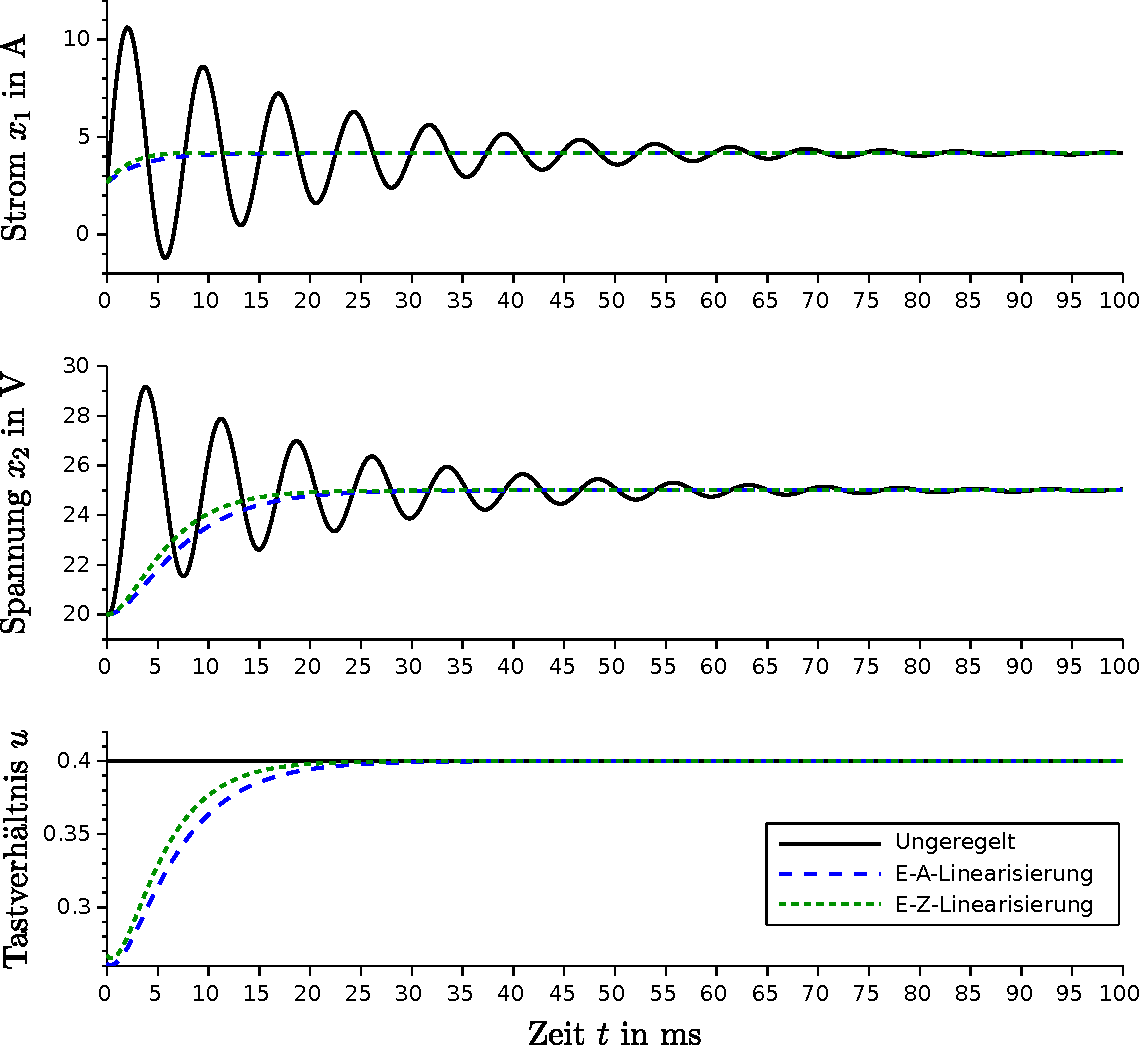
\includegraphics[width=0.9\textwidth]{Hochsetzsteller_Simulation}
\par\end{centering}
\caption{Simulation des gemittelten Hochsetzstellers\label{fig:Simulation-Hochsetzsteller}}
\end{figure}

\bibliographystyle{babalpha}
\bibliography{dynamic}

